\documentclass[12pt]{ucsddissertation}
% mathptmx is a Times Roman look-alike (don't use the times package)
% It isn't clear if Times is required. The OGS manual lists several
% "standard fonts" but never says they need to be used.
\usepackage{mathptmx}
\usepackage[numbers]{natbib}
\usepackage[NoDate]{currvita}
\usepackage{array}
\usepackage{tabularx}
\usepackage{booktabs}
\usepackage{ragged2e}
\usepackage{microtype}
\usepackage{xcolor}
\usepackage[breaklinks=true,pdfborder={0 0 0}]{hyperref}
\usepackage{graphicx}
\usepackage{amsmath, amsfonts, amssymb}
\usepackage{dsfont}
\usepackage{nicefrac}
\usepackage{mathtools}
\usepackage[ruled, lined, linesnumbered, commentsnumbered, longend]{algorithm2e}
\usepackage{amsthm}
\usepackage{wrapfig}
\usepackage{geometry}
\usepackage{soul}
\usepackage{lipsum}
\usepackage{tikz}
\usetikzlibrary{bayesnet}
\usepackage{bbm}
\usepackage{subcaption}
\usepackage{yfonts}
\captionsetup[sub]{font=scriptsize,labelfont={bf}}
\usepackage[breakable, theorems, skins]{tcolorbox}
\usepackage[capitalize,noabbrev]{cleveref}
\AtBeginDocument{%
	\settowidth\cvlabelwidth{\cvlabelfont 0000--0000}%
}

\DeclareMathOperator*{\argmax}{arg\,max}
\DeclareMathOperator*{\argmin}{arg\,min}

% OGS recommends increasing the margins slightly.
\increasemargins{.1in}

% These are just for testing/examples, delete them
\usepackage{trace}
%\usepackage{showframe} % This package was just to see page margins
\usepackage[english]{babel}
\usepackage{blindtext}
\overfullrule5pt
% ---

%%For multi-file compilation 
%\usepackage{subfiles}

% Required information
\title{Theoretical Foundations of Trustworthy Machine Learning}
\author{Robi Bhattacharjee}
\degree{Computer Science}{Doctor of Philosophy}
% Each member of the committee should be listed as Professor Foo Bar.
% If Professor is not the correct title for one, then titles should be
% omitted entirely.
\chair{Professor Kamalika Chaudhuri}
% Your committee members (other than the chairs) must be in alphabetical order
\committee{Professor Mikhail Belkin}
\committee{Professor Sanjoy Dasgupta}
\committee{Professor Yoav Freund}

\degreeyear{2023}


% Start the document
\begin{document}
% Begin with frontmatter and so forth
\frontmatter
\maketitle
\makecopyright
\makesignature
% Optional
\begin{dedication}
\setsinglespacing
\raggedright % It would be better to use \RaggedRight from ragged2e
\parindent0pt\parskip\baselineskip
For Mom, Dad, and Sormeh.  
\end{dedication}

%% Optional
%\begin{epigraph}
%\vskip0pt plus.5fil
%\setsinglespacing
%%{\flushright
%%True ease in writing comes from art, not chance,\\
%%As those move easiest who have learn'd to dance.\\
%%'T is not enough to no harshness gives offence,---\\
%%The sound must seem an echo to the sense.
%%
%%\vskip\baselineskip
%%\textit{Alexander Pope}\par}
%\vfil
%\begin{center}
%Something pithy
%
%\vskip\baselineskip
%\textit{Someone smart}
%\end{center}
%\vfil
%%\noindent Writing, at its best, is a lonely life. Organizations for
%%writers palliate the writer's loneliness, but I doubt if they improve
%%his writing. He grows in public stature as he sheds his loneliness and
%%often his work deteriorates. For he does his work alone and if he is a
%%good enough writer he must face eternity, or the lack of it, each day.
%%
%%\vskip\baselineskip
%%\hskip0pt plus1fil\textit{Ernest Hemingway}\hskip0pt plus4fil\null
%
%%\vfil
%\end{epigraph}

% Next comes the table of contents, list of figures, list of tables,
% etc. If you have code listings, you can use \listoflistings (or
% \lstlistoflistings) to have it be produced here as well. Same with
% \listofalgorithms.
\tableofcontents
\listoffigures
\listoftables

%% Preface
%\begin{preface}
%Almost nothing is said in the manual about the preface. There is no
%indication about how it is to be typeset. Given that, one is forced to
%simply typeset it and hope it is accepted. It is, however, optional
%and may be omitted.
%\end{preface}

% Your fancy acks here. Keep in mind you need to ack each paper you
% use. See the examples here. In addition, each chapter ack needs to
% be repeated at the end of the relevant chapter.
\begin{acknowledgements}
%Above all, I thank my advisor, Kamalika, for her mentorship over the last five years. Kamalika will do anything in her power to help her students find what success means to them, and build towards it. She puts her students' futures above all else. Part of that is mentoring her students to become thoughtful researchers. In hindsight, I see that we could have pursued much lower risk projects that made incremental gains on the hottest research directions. Instead, Kamalika guided me towards unusual and challenging problems that required me to examine my fundamentals and reconsider broad questions about the aims of data privacy. In doing so, I not only understand what solutions are effective in data privacy, but why we as a research community use them and --- in some cases --- why we have ignored them. 
%
%I cannot overemphasize the gratitude I have to my collaborators as well. First, to my collaborators at FAIR. I thank Chuan Guo for showing me how to navigate incredibly challenging and open-ended ML problems. His Socratic approach to mentoring helped me explore my own instincts and take ownership of the project without letting me slip down the wrong path. Florian Bordes taught me the ins and outs of contemporary vision modeling. Pascal Vincent's insights on how to design deep learning experiments were truly formative; I sincerely appreciate his effort and time. I owe an enormous debt of gratitude to Ashwin Machanavajjhala at Tumult for mentoring me on how how to reason about different privacy definitions and guarantees in applied settings. 
%
%Finally, to all of my friends. To the lab: I could not have landed in a better group. To be surrounded by such wonderful and bright companions is a win --- for them to be your colleagues as well is a gift. To all my dear pre-PhD friends (you know who you are, and you really don't have read this dissertation): you are the loves of my life! 

%\pagebreak
%
%\textbf{Chapter 1}, in full, has been submitted for publication of the material
%as it may appear in Neural Information Processing Systems,~2023, Casey Meehan, Florian Bordes, Pascal Vincent, Kamalika Chaudhuri, Chuan Guo. \emph{Do SSL models have Déjà Vu? A Case of Unintended Memorization in Self-Supervised Learning}. The dissertation author shares equal contribution with Florian Bordes. 
%
%\textbf{Chapter 2}, in full, is a reprint of the material as it appears in International Conference on Artificial Intelligence and Statistics, 2020. Casey Meehan, Sanjoy Dasgupta, Kamalika Chaudhuri. \emph{A Non-parametric Test to Detect Data-Copying in Generative Models}. The dissertation author is the primary investigator and author of this paper. 
%
%\textbf{Chapter 3}, in full, is a reprint of the material as it appears in Proceedings of the 60th Annual Meeting of the Association for Computational Linguistics (Volume 1: Long Papers), 2022. Casey Meehan, Khalil Mrini, Kamalika Chaudhuri. \emph{Sentence-level Privacy for Document Embeddings}. The dissertation author is the primary investigator and author of this paper. 
%
%\textbf{Chapter 4}, in full, is a reprint of the material as it appears in International Conference on Learning Representations. 2022. Casey Meehan, Amrita Roy-Chowdhury, Kamalika Chaudhuri, Somesh Jha. \emph{Privacy Implications of Shuffling}. The dissertation author is the primary investigator and author of this paper.
%
%\textbf{Chapter 5}, in full, is a reprint of the material as it appears in International Conference on Artificial Intelligence and Statistics, 2021. Casey Meehan, Kamalika Chaudhuri. \emph{Location Trace Privacy Under Conditional Priors}. The dissertation author is the primary investigator and author of this paper. 
\end{acknowledgements}

% Stupid vita goes next
\begin{vita}
\noindent
\begin{cv}{}
\begin{cvlist}{}
\item[2016] Bachelor of Science, Massachusetts Institute of Technology
\item[2022] Master of Science, University of California, San Diego
\item[2023] Doctor of Philosophy, University of California, San Diego
\end{cvlist}
\end{cv}

%% This puts in the PUBLICATIONS header. Note that it appears inside
%% the vita environment. It is optional.
%\publications
%\noindent``Distributions of Control Points in a System for Analysis of Stress
%Distribution'' IRE Transactions of the I.R.E\@. Professional Group on
%Automatic Control, vol. AC-7, pp 272--289, September 2005

%% This puts in the FIELDS OF STUDY. Also inside vita and also
%% optional.
%\fieldsofstudy
%\noindent Major Field: Engineering (Specialization or Focused Studies)
%\vskip\baselineskip
%Studies in Applied Mathematics\par
%Professors Alpha Beta and Gamma Delta
%\vskip\baselineskip
%Studies in Mechanices\par
%Professors Epsilon Zeta and Eta Theta
%\vskip\baselineskip
%Studies in Electromagnetism\par
%Professors Iota Kappa and Lambda Mu
\end{vita}

% Put your maximum 350 word abstract here.
\begin{dissertationabstract}
%The Abstract begins here. The abstract is limited to 350 words for a
%doctoral dissertation. It should consist of a short statement of the
%problem, a brief explanation of the methods and procedures employed in
%generating the data, and a condensed summary of the findings of the
%study. The abstract may continute onto a second page if necessary. The
%text of the abstract must be double spaced.
As data collection for machine learning (ML) tasks has become more pervasive, it has also become more heterogeneous: we share our writing, images, voices, and location online every day. Naturally, the associated privacy risks are just as complex and variable. My research advances practical data privacy through two avenues: 1) drafting provable privacy definitions and mechanisms for safely sharing data in different ML domains, and 2) empirically quantifying how ML models memorize their sensitive training data and thereby risk disclosing it. This dissertation details the various data domains/tasks considered, and the corresponding privacy methods proposed. 
\end{dissertationabstract}

% This is where the main body of your dissertation goes!
\mainmatter

% Optional Introduction
\begin{dissertationintroduction}
In recent years, there has been an explosion of machine learning applications ranging from (partially) self-driving cars to large language models such as ChatGPT. These models are becoming an increasingly prevalent part of society, and it is therefore crucial that they are deployed in a safe and reliable way.

Classical machine learning theory, which forms the basis upon which much of this technology is built, typically involves a formalism in which the learner is given input data and asked to solve a specific task. For example, in the statistical learning framework for classification, the learner is given training data and asked to output a classifier with the highest possible accuracy. However, specific approaches such as this often fail to capture the multitude of behaviors and features that are necessary for broader applications of machine learning. Indeed, performing well on test data is far from a sufficient condition for a model to be deployable in the real world. 

This dissertation attempts towards building theoretical foundations that are able to address machine learning in this broader context by considering two specific problems in reliable machine learning, \textit{adversarial examples,} and \textit{data copying.}


\textbf{Adversarial examples.} Adversarial examples arise in classification, and are small imperceptible changes to a given input that are designed to cause misclassification. For example, a malicious actor might try to circumvent a spam filter by finding perturbations that fool the filter but nevertheless preserve the essence of their content. To remedy this, there has been a growing focus on building \textit{robust} classifiers for which adversarial examples cannot exist.

In the first two chapters of this dissertation, we study this problem in the non-parametric setting and seek to understand under what conditions non-parametric algorithms output classifiers that are both accurate and robust. In the next two chapters, we consider linear classification and seek to understand whether robust classification intrinsically requires more data than simply focusing on accuracy does.

\textbf{Data Copying.} Next, we switch gears and consider a problem in reliable \textit{generative modeling.} Prior work (i.e. \cite{lopez2016revisiting,XHYGSWK18}) has found that large generative models often appear to memorize their training data and often output a near copy of one of their training points when queried. In addition to posing clear security risks with respect to privacy or copyright violations, such "data-copying" also indicates poor generalization and limited usefulness. In the last chapter of this dissertation, we propose a formal definition of data-copying and give the first algorithm with provable guarantees for detecting it. 



%The privacy risks and utility requirements of each of these settings and applications warrant different approaches to privacy-preserving ML. This dissertation proposes a variety of solutions to situations like those above. In doing so, I hope to illuminate the advantage of taking an application-specific approach to both measuring privacy risks and engineering private algorithms. The following five chapters are roughly organized into two parts: the first two chapters cover \emph{empirical} privacy methods, and the remaining three cover \emph{formal} privacy methods. The former includes statistical tests to quantify privacy risks of large ML models. The latter proposes provably private algorithms to satisfy different privacy definitions chosen for different ML tasks. 
%
%\textbf{Empirical methods.} The first two chapters explore empirically measuring privacy risks in the domain of vision modeling. In both chapters, we analyze to what extent large vision models \emph{memorize} their training images, and thereby risk exposing them. In contrast with the following three chapters, we are not proposing a provably privacy-preserving algorithm. Instead we are designing methodical empirical tests to quantify memorization. 
%
%\textbf{Provably private algorithms.} The final three chapters propose algorithms that allow us to share our data in a provably private way. We explore privacy preserving algorithms in the text, location, and interpersonal-correlated domains (\emph{e.g.} social networks or genetically linked medical data). For each of these, we study different ML tasks and privacy risks to motivate different privacy definitions and provably private algorithms. 
%
%Taken together, this document offers a mindset towards practicable privacy methods. By directly considering the data domain and the task at hand, it is possible to efficiently measure privacy risks and propose provably private algorithms while still completing the learning task at hand .  
\end{dissertationintroduction}

%\chapter{An ordinary page}
%The purpose of this page is to illustrate an ordinary page of text in
%a doctoral dissertation or master's thesis. All pages of the doctoral
%dissertation or master's thesis must be kept within the margins of
%1.5'' on the left, 1'' on the right, 1'' on the top and 1.25'' on the
%bottom. All text must be double spaced except as indicated below.
%
%It is recommended that to increase the margins as paper can shift in a
%printer and as some photocopiers tend to increase the image being
%copied.
%
%The first line of each paragraph must be indented at least one 0.5''
%tab, as done here.
%
%This text is intended to be a part of the dissertation, for a doctoral
%student, or the thesis if you are receiving a master's degree, and now
%a quote is included here:
%\begin{quote}
%All quotes of more than six lines, even though this one is not, are to
%be indented 0.5'' from the left and 0.5'' from the right. These longer
%quotes are to be single spaced. Don't forget to adjust for proper
%spacing after the last line of the quoted material.
%\end{quote}
%The rest of the paragraph would continue as so.

\graphicspath{{./chapters/chapter0/}}
\chapter{When are Non-Parametric Methods Robust?} 

\newtheorem{thm}{Theorem}
\newtheorem{lem}[thm]{Lemma}
\newtheorem{cor}[thm]{Corollary}

\newtheorem{defn}[thm]{Definition}
\newtheorem{ex}{Example}

\def\D{{\mathcal D}}
\def\X{\mathcal X}
\def\R{\mathbb R}
\def\Y{\{\pm 1\}}
\def\w{\hat{w}}
\def\P{\mathbb{P}}
\def\I{\hat{I}}
\def\b{g^*}
\def\r{\rho}
\def\rcons{r-consistent}
\def\rconsy{r-consistency}
\def\ap{AdvPrun}
\def\ga{RobustNonPar}

\section{Introduction}

Recent work has shown that many classifiers tend to be highly non-robust and that small strategic modifications to regular test inputs can cause them to misclassify~\cite{Szegedy14, Goodfellow14, MeekLowd05}. Motivated by the use of machine learning in safety-critical applications, this phenomenon has recently received considerable interest; however, what exactly causes this phenomenon -- known in the literature as {\em{adversarial examples}} -- still remains a mystery.

Prior work has looked at three plausible reasons why adversarial examples might exist. The first, of course, is the possibility that in real data distributions, different classes are very close together in space -- which does not seem plausible in practice. Another possibility is that classification algorithms may require more data to be robust than to be merely accurate; some prior work~\cite{Madry18, WJC18, Srebro19} suggests that this might be true for certain classifiers or algorithms. Finally, others~\cite{Bubeck19, Vinod19, WJC18} have suggested that better training algorithms may give rise to more robust classifiers -- and that in some cases, finding robust classifiers may even be computationally challenging.

In this work, we consider this problem in the context of general non-parametric classifiers. Contrary to parametrics, non-parametric methods are a form of local classifiers, and include a large number of pattern recognition methods such as nearest neighbors, decision trees, random forests and kernel classifiers. There is a richly developed statistical theory of non-parametric methods~\cite{devroye96}, which focuses on accuracy, and provides very general conditions under which these methods converge to the Bayes optimal with growing number of samples. We, in contrast, analyze robustness properties of these methods, and ask instead when they converge to the classifier with the highest astuteness at a desired radius $r$. Recall that the astuteness of a classifier at radius $r$ is the fraction of points from the distribution on which it is accurate and has the same prediction up to a distance $r$~\cite{WJC18, Madry18}.

 We begin by looking at the very simple case when data from different classes is well-separated -- by at least a distance $2r$. Although achieving astuteness in this case may appear trivial, we show that even in this highly favorable case, not all non-parametric methods provide robust classifiers -- and this even holds for methods that converge to the Bayes optimal in the large sample limit.  

This raises the natural question -- when do non-parametric methods produce astute classifiers? We next provide conditions under which a non-parametric method converges to the most astute classifier in the large sample limit under well-separated data. Our conditions are analogous to the classical conditions for convergence to the Bayes optimal~\cite{devroye96, Stone77}, but a little stronger. We show that nearest neighbors and kernel classifiers whose kernel functions decay fast enough, satisfy these conditions, and hence converge to astute classifiers in the large sample limit. In constrast, histogram classifiers, which do converge to the Bayes optimal in the large sample limit, may not converge to the most astute classifier. This indicates that there may be some non-parametric methods, such as nearest neighbors and kernel classifiers, that are more naturally robust when trained on well-separated data, and some that are not.

What happens when different classes in the data are not as well-separated? For this case, \cite{YRWC19} proposes a method called Adversarial Pruning that preprocesses the training data by retaining the maximal set of points such that different classes are distance $\geq 2r$ apart, and then trains a non-parametric method on the pruned data. We next prove that if a non-parametric method has certain properties, then the classifier produced by Adversarial Pruning followed by the method does converges to the most astute classifier in the large sample limit. We show that again nearest neighbors and kernel classifiers whose kernel functions decay faster than inverse polynomials satisfy these properties. Our results thus complement and build upon the empirical results of~\cite{YRWC19} by providing a performance guarantee. 

What can we conclude about the cause for adversarial examples? Our results seem to indicate that at least for non-parametrics, it is mostly the training algorithms that are responsible. With a few exceptions, decades of prior work in machine learning and pattern recognition has largely focussed on designing training methods that provide increasingly accurate classifiers -- perhaps to the detriment of other aspects such as robustness. In this context, our results serve to (a) provide a set of guidelines that can be used for designing non-parametric methods that are robust and accurate on well-separated data and (b) demonstrate that when data is not well-separated, preprocessing through adversarial pruning~\cite{YRWC19} may be used to ensure convergence to optimally astute solutions in the large sample limit. 

\subsection{Related Work}

There is a large body of work on adversarial attacks~\cite{Carlini17, Liu17, Papernot17, Papernot16,Szegedy14} and defenses~\cite{Hein17,Katz17,Schmidt18,Wu16,Steinhardt18, Sinha18} in the parametric setting, specifically focusing on neural networks. On the other hand, adversarial examples for nonparametric classifiers have mostly been studied in a much more ad-hoc manner, and to our knowledge, there has been no theoretical investigation into general properties of algorithms that promote robustness in non-parametric classifiers.

For nearest neighbors, there has been some prior work on adversarial attacks~\cite{Amsaleg17, Sitawarin19, WJC18, YRWC19} as well as defenses. Wang et. al. \cite{WJC18} proposes a defense for 1-NN by pruning the input sample. However, their defense learns a classifier whose robustness regions converge towards those of the Bayes optimal classifier, which itself may potentially have poor robustness properties. Yang et. al. \cite{YRWC19} accounts for this problem by proposing the notion of the $r$-optimal classifier, and propose an algorithm called Adversarial Pruning which can be interpreted as a finite sample approximation to the $r$-optimal. However, they do not provide formal performance guarantees for Adversarial Pruning, which we do. 

For Kernel methods, Hein and Andriushchenko \cite{Hein17} study lower bounds on the norm of the adversarial manipulation that is required for changing a classifiers output. They specifically study bounds for Kernel Classifiers, and propose an empirically based regularization idea that improves robustness. In this work, we improve the robustness properties of kernel classification through adversarial pruning, and show formal guarantees regarding convergence towards the $r$-optimal classifier. 

For decision trees and random forests, attacks and defenses have been provided by \cite{Hein19, Kantchelian15, Hsiehicml19}. Again, most of the work here is empirical in nature, and convergence guarantees are not provided. 

Pruning has a long history of being applied for improving nearest neighbors \cite{Gates72, Gottlieb14, Hart68, KontorovichSW17, KontorovichW15, Hanneke19}, but this has been entirely done in the context of generalization, without accounting for robustness. In their work, Yang et. al. empirically show that adversarial pruning can improve robustness for nearest neighbor classifiers. However, they do not provide any formal guarantees for their algorithms. In this work, we prove formal guarantees for \textit{adversarial pruning} in the large sample limit, both for nearest neighbors as well as for more general \textit{weight functions.} 

There is a long history of literature for understanding the consistency of Kernel classifiers \cite{Steinwart05, Stone77}, but this has only been done for accuracy and generalization. In this work, we find different conditions are needed to ensure that a Kernel classifier converges in robustness in addition to accuracy.

\section{Preliminaries}

\subsection{Setting}
We consider binary classification where instances are drawn from a totally bounded metric space $\X$ that is equipped with distance metric denoted by $d$, and the label space is $\Y = \{ -1, +1 \}$. The classical goal of classification is to build a highly \textit{accurate} classifier, which we define as follows.

\begin{defn}
(Accuracy) Let $\D$ be a distribution over $\X \times \Y$, and let $f \in \Y^\X$ be a classifier. Then the \textbf{accuracy} of $f$ over $\D$, denoted $A(f, \D)$, is the fraction of examples $(x,y) \sim \D$ for which $f(x) = y$. Thus $$A(f, \D) = P_{(x,y) \sim \D}[f(x) = y].$$
\end{defn}

In this work, we consider \textit{robustness} in addition to accuracy. Let $B(x,r)$ denoted the closed ball of radius $r$ centered at $x$. 

\begin{defn}
(Robustness) A classifier $f \in \Y^\X$ is said to be \textbf{robust} at $x$ with radius $r$ if $f(x) = f(x')$ for all $x' \in B(x,r)$.
\end{defn}

Our goal is to find non-parametric algorithms that output classifiers that are robust, in addition to being accurate. To account for both criteria, we combine them into a notion of \textit{astuteness}~\cite{WJC18, Madry18}. 

\begin{defn}
(Astuteness) A classifier $f \in \Y^\X$ is said to be \textbf{astute} at $(x,y)$ with radius $r$ if $f$ is robust at $x$ with radius $r$ and $f(x) = y$. The \textbf{astuteness} of $f$ over $\D$, denoted $A_r(f, \D)$, is the fraction of examples $(x,y) \sim \D$ for which $f$ is astute at $(x,y)$ with radius $r$. Thus $$A_r(f, \D) = P_{(x, y) \sim \D}[f(x') = y, \forall x' \in B(x,r)].$$
\end{defn}

It is worth noting that $A_0(f, \D) = A(f, \D)$, since astuteness with radius $0$ is simply the accuracy. For this reason, we will use $A_0(f, \D)$ to denote accuracy from this point forwards.

\subsection{Notions of Consistency}

Traditionally, a classification algorithm is said to be consistent if as the sample size grows to infinity, the accuracy of the classifier it learns converges towards the best possible accuracy on the underlying data distribution. We next introduce and formalize an alternative form of consistency, called $r$-consistency, that applies to robust classifiers.

We begin with a formal definition of the Bayes Optimal Classifier -- the most accurate classifier on a distribution -- and consistency. 

\begin{defn}
(Bayes Optimal Classifier) The \textbf{Bayes Optimal Classifier} on a distribution $\D$, denoted by $\b$, is defined as follows. Let $\eta(x) = p_\D(+1|x)$. Then
 \[ \b(x) = \begin{cases} 
      +1 & \eta(x) \geq 0.5 \\
      -1 & \eta(x) < 0.5 \\
   \end{cases}
\]
It can be shown that $\b$ achieves the highest accuracy over $\D$ over all classifiers.
\end{defn}

\begin{defn}
(Consistency) Let $M$ be a classification algorithm  over $\X \times \Y$. $M$ is said to be \textbf{consistent} if for any $\D$ over $\X \times \Y$, and any $\epsilon, \delta$ over $(0,1)$, there exists $N$ such that for $n \geq N$, with probability $1-\delta$ over $S \sim \D^n$, we have: $$A(M(S), \D) \geq A(\b, \D) - \epsilon,$$ where $\b$ is the Bayes optimal classifier for $\D$. 
\end{defn}

How can we incorporate robustness in addition to accuracy in this notion? A plausible way, as used in~\cite{WJC18}, is that the classifier should converge towards being astute where the Bayes Optimal classifier is astute. However, the Bayes Optimal classifier is not necessarily the most astute classifier and may even have poor astuteness. To see this, consider the following example. 

\paragraph{Example 1}
Consider $\D$ over $\X = [0,1]$ such that $\D_\X$ is the uniform distribution and $$p(y=1|x) = \frac{1}{2} + \sin \frac{4 \pi x}{r}.$$ For any point $x$, there exists $x_1, x_2 \in ([x-r, x+r] \cap [0,1])$ such that $p(y=1|x_1) > \frac{1}{2}$ and $p(y=1|x_2) < \frac{1}{2}$. $A_r(\b, r) = 0$. However, the classifier that always predicts $f(x) = +1$ does better. It is robust everywhere, and since $P_{(x,y) \sim \D}[y = +1] = \frac{1}{2}$, it follows that $A_r(f, \D) = \frac{1}{2}$. \\ \\

This motivates the notion of the $r$-optimal classifier, introduced by~\cite{YRWC19}, which is the classifier with maximum astuteness. 

\begin{defn}
($r$-optimal classifier) The \textbf{$r$-optimal classifier} of a distribution $G$ denoted by $\b_r$ is the classifier with maximum astuteness. Thus $$\b_r = \argmax_{f \in \Y^\X} A_r(f, \D).$$ We let $A_r^*(\D)$ denote $A_r(\b_r, \D)$. 
\end{defn}

Observe that $\b_r$ is not necessarily unique. To account for this, we use $A_r^*(\D)$ in our definition for \rconsy. 

\begin{defn} \label{defn_archons}
(\rcons) Let $M$ be a classification algorithm over $\X \times \Y$. $M$ is said to be \textbf{\rcons} if for any $\D$,  any $\epsilon, \delta \in (0,1)$, and $0 < \gamma < r$, there exists $N$ such that for $n \geq N$, with probability $1-\delta$ over $S \sim \D^n$, $$A_{r-\gamma}(M(S), \D) \geq A_r^*(\D) - \epsilon.$$ if the above conditions hold for a specific distribution $\D$, we say that $M$ is \rcons\emph{ }with respect to $\D$. 
\end{defn}

Observe that in addition to the usual $\epsilon$ and $\delta$, there is an extra parameter $\gamma$ which measures the gap in the robustness radius. We may need this parameter as when classes are exactly $2r$ apart, we may not be able to find the exact robust boundary with only finite samples. 

Our analysis will be centered around understanding what kinds of algorithms $M$ provide highly astute classifiers for a given radius $r$. We begin by first considering the special case of \textit{$r$-separated} distributions. 

\begin{defn}
($r$-separated distributions) A distribution $\D$ is said to be \textbf{$r$-separated} if there exist subsets $T^+, T^- \subset \X$ such that 
\begin{enumerate}
	\item $\P_{(x,y) \sim \D}[x \in T^y] = 1$. 
	\item $\forall x_1 \in T^+, \forall x_2 \in T^-$, $d(x_1, x_2) > 2r$.
\end{enumerate}
\end{defn}

Observe that if $\D$ is $r$-separated, $A_r(\b_r, \D) = 1$.

\subsection{Non-parametric Classifiers}\label{classifiers}

Many non-parametric algorithms classify points by averaging labels over a local neighborhood from their training data. A very general form of this idea is encapsulated in \textit{weight functions} -- which is the general form we will use.

\begin{defn} \label{def:weight}
\cite{devroye96} A \textbf{weight function} $W$ is a non-parametric classifier with the following properties.
\begin{enumerate}
	\item Given input $S = \{(x_1, y_1), (x_2, y_2,), \dots, (x_n, y_n)\} \sim \D^n$, $W$ constructs functions $w_1^S, \dots, w_n^S: \X \to [0, 1]$ such that for all $x \in \X$, $\sum_1^n w_i^S(x) = 1$. The functions $w_i^S$ are allowed to depend on $x_1, x_2, \dots x_n$ but must be independent of $y_1, y_2, \dots, y_n$. 
	\item $W$ has output $W_S$ defined as \[ W_S(x) = \begin{cases} 
      +1 & \sum_1^n w_i^S(x)y_i > 0 \\
      -1 & \sum_1^n w_i^S(x)y_i \leq 0 \\
   \end{cases}
\]
As a result, $w_i^S(x)$ can be thought of as the weight that $(x_i, y_i)$ has in classifying $x$.
\end{enumerate}
\end{defn}

Weight functions encompass a fairly extensive set of common non-parametric classifiers, which is the motivation for considering them. We now define several common non-parametric algorithms that can be construed as weight functions. 

\begin{defn}
A \textbf{histogram classifier}, $H$, is a non-parametric classification algorithm over $\R^d \times \Y$ that works as follows. For a distribution $\D$ over $\R \times \Y$, $H$ takes $S = \{(x_i, y_i): 1 \leq i \leq n\} \sim \D^n$ as input. Let $k_i$ be a sequence with $\lim_{i \to \infty} k_i = \infty$ and $\lim_{i \to \infty} \frac{k_i}{i} = 0$. $H$ constructs a set of hypercubes $C = \{c_1, c_2, \dots, c_m\}$ as follows:
\begin{enumerate}
	\item Initially $C = \{c\}$, where $S \subset c$.
	\item For $c \in C$, if $c$ contains more than $k_n$ points of $S$, then partition $c$ into $2^d$ equally sized hypercubes, and insert them into $C$.
	\item Repeat step $2$ until all cubes in $C$ have at most $k_n$ points. 
\end{enumerate}
For $x \in \R$ let $c(x)$ denote the unique cell in $C$ containing $x$. If $c(x)$ doesn't exist, then $H_S(x) = -1$ by default. Otherwise, \[ H_S(x) = \begin{cases} 
      +1 & \sum_{x_i \in c(x)} y_i > 0 \\
      -1 & \sum_{x_i \in c(x)}y_i \leq 0 \\
   \end{cases}.
\]
\end{defn}

Histogram classifiers are weight functions in which all $x_i$ contained within the same cell as $x$ are given the same weight $w_i^S(x)$ in predicting $x$, while all other $x_i$ are given weight $0$. 

\begin{defn}
A \textbf{kernel classifier} is a weight function $W$ over $\X \times \Y$ constructed from function $K: \R^+ \cup \{0\} \to \R^+$ and some sequence $\{h_n\} \subset \R^+$ in the following manner. Given $S = \{(x_i, y_i)\} \sim \D^n$, we have $$w_i^S(x) = \frac{K(\frac{d(x, x_i)}{h_n})}{\sum_{j = 1}^n K(\frac{d(x, x_j)}{h_n})}.$$ Then, as above, $W$ has output \[ W_S(x) = \begin{cases} 
      +1 & \sum_1^n w_i^S(x)y_i > 0 \\
      -1 & \sum_1^n w_i^S(x)y_i \leq 0 \\
   \end{cases}
\]
\end{defn}

Finally, we note that $k_n$-nearest neighbors is also a weight function; $w_i^S(x) = \frac{1}{k_n}$ if $x_i$ is one of the $k_n$ closest neighbors of $x$ and $0$ otherwise.

\section{Warm Up: $r$-separated distributions}

We begin by considering the case when the data distribution is $r$-separated; the more general case is considered in Section~\ref{sec:general}. While classifying $r$-separated distributions robustly may appear almost trivial, learning an arbitrary classifier does not necessarily produce an astute result. To see this, consider the following example of a histogram classifier -- which is known to be consistent. 


We let $H$ denote the histogram classifier over $\R$.

\paragraph{Example 2}
Consider the data distribution $\D = \D^+ \cup \D^-$ where $D^+$ is the uniform distribution over $[0, \frac{1}{4})$ and $D^-$ is the uniform distribution over $(\frac{1}{2}, 1]$, $p(+1|x) = 1$ for $x \in \D^+$, and $p(-1|x) = 1$ for $x \in \D^-$. 

We make the following observations (refer to Figure \ref{fig:histogram}).
\begin{enumerate}
	\item $\D$ is $0.1$-separated, since the supports of $\D^+$ and $\D^-$ have distance $0.25 > 0.2$. 
	\item If $n$ is sufficiently large, $H$ will construct the cell $[0.25, 0.5)$, which will not be split because it will never contain any points. 
	\item $H_S(x) = -1$ for $x \in [0.25, 0.5)$.
	\item $H_S$ is not astute at $(x,1)$ for $x \in (0.15, 0.25)$. Thus $A_{0.1}(H_S, \D) = 0.8$.
\end{enumerate}

\begin{figure}
\centering
\definecolor{dtsfsf}{rgb}{0.8274509803921568,0.1843137254901961,0.1843137254901961}
\definecolor{sexdts}{rgb}{0.1803921568627451,0.49019607843137253,0.19607843137254902}
\begin{tikzpicture}[line cap=round,line join=round,>=triangle 45,x=1cm,y=1cm]
\clip(-4.68,0) rectangle (2.46,3);
\draw [line width=2pt] (-3.8971542001619626,1.7601524817792173)-- (-3.90319974718047,1.0800284421971598);
\draw [line width=2pt] (-2.7721542001619626,1.7501524817792171)-- (-2.7781997471804694,1.0700284421971598);
\draw [line width=2pt] (-1.6471542001619623,1.7401524817792173)-- (-1.6531997471804694,1.0600284421971597);
\draw [line width=2pt] (0.6028457998380374,1.720152481779217)-- (0.5968002528195302,1.0400284421971597);
\draw [line width=2pt] (-2.775,1.43)-- (-1.65,1.42);
\draw [line width=2pt,color=sexdts] (-1.65,1.42)-- (0.6,1.4);
\draw [line width=2pt,color=sexdts] (-3.9,1.44)-- (-3.2002330680045032,1.4337798494933733);
\draw [line width=2pt,color=dtsfsf] (-3.2002330680045032,1.4337798494933733)-- (-2.775,1.43);
\draw (-3.54,2.48) node[anchor=north west] {$\mathcal{D}^+$};
\draw (-0.76,2.46) node[anchor=north west] {$\mathcal{D}^-$};
\draw (-4,1.1) node[anchor=north west] {0};
\draw (-3.14,1.08) node[anchor=north west] {0.25};
\draw (-1.86,1.1) node[anchor=north west] {0.5};
\draw (0.5,1.08) node[anchor=north west] {1};
\end{tikzpicture}
\caption{$H_S$ is astute in the green region, but not robust in the red region.} \label{fig:histogram}
\end{figure}

Example 2 shows that histogram classifiers do not always learn astute classifiers even when run on $r$-separated distributions. This motivates the question: which non-parametric classifiers do?

We answer this question in the following theorem, which gives sufficient conditions for a weight function (definition \ref{def:weight}) to be $r$-consistent over an $r$-separated distribution.

\begin{thm}\label{thm_stone_cons}
Let $\D$ be a distribution over $\X \times \Y$, and let $W$ be a weight function. Let $X$ be a random variable with distribution $\D_\X$, and $S = \{(x_1, y_1), (x_2, y_2), \dots, (x_n, y_n)\} \sim \D^n$. Suppose that for any $0 < a < b,$ $$\lim_{n \to \infty} \mathbb{E}_{X, S} \big [ \sup_{x' \in B(X, a)} \sum_1^n w_i^S(x')I_{||x_i - x'|| > b} \big] = 0.$$  Then if $\D$ is $r$-separated, $W$ is \rcons\emph{ } with respect to $\D$.  
\end{thm}

First, we compare Theorem \ref{thm_stone_cons} to Stone's theorem \cite{Stone77}, which gives sufficient conditions for a weight function to be consistent (i.e. converge in accuracy towards the Bayes optimal). For convenience, we include a statement of Stone's theorem. 
\begin{thm}\label{thm_stone}
\cite{Stone77} Let $W$ be weight function over $\X \times \Y$. Suppose the following conditions hold for any distribution $\D$ over $\X \times \Y$.  Let $X$ be a random variable with distribution $\D_\X$, and $S = \{(x_1, y_1), (x_2, y_2), \dots, (x_n, y_n)\} \sim \D^n$. All expectations are taken over $X$ and $S$. 
\begin{enumerate}
	\item There is a constant $c$ such that, for every nonnegative measurable function $f$ satisfying $\mathbb{E} [f(X)] < \infty$, $$\mathbb{E} [\sum_1^n w_i^S(X)f(x_i)] \leq c \mathbb{E} [f(x)].$$
	\item For all $a > 0$, $$\lim_{n \to \infty} \mathbb{E}[\sum_1^n w_i^S(x)I_{||x_i - X|| > a}] = 0,$$ where $I_{||x_i - X|| > a}$ is an indicator variable. 
	\item $$\lim_{n \to \infty} \mathbb{E}[\max_{1 \leq i \leq n} w_i^S(X)] = 0.$$
\end{enumerate}
Then $W$ is consistent. 
\end{thm}
There are two main differences between Theorem \ref{thm_stone_cons} and Stone's theorem.
 \begin{enumerate}
 	\item Conditions 1. and 3. of Stone's theorem are no longer necessary. This is because $r$-separated distributions are well-separated and thus have simpler conditions for consistency. In fact, a slight modification of the arguments of~\cite{Stone77} shows that for $r$-separated distributions, condition 2. alone is sufficient for consistency.
 	\item Condition 2. is strengthened. Instead of requiring the weight of $x_i$'s outside of a given radius to go to $0$ for $X \sim \D$, we require the same to \textit{uniformly} hold over a ball centered at $X$. 
\end{enumerate}  
 


Theorem \ref{thm_stone_cons} provides a general condition that allows us to verify the $r$-consistency of non-parametric methods. We now show below that two common non-parametric algorithms -- $k_n$-nearest neighbors and kernel classifiers with rapidly decaying kernel functions -- satisfy the conditions of Theorem~\ref{thm_stone_cons}.
 
\begin{cor}\label{nn_sep_thm}
Let $\D$ be any $r$-separated distribution. Let $k_n$ be any sequence such that $\lim_{n \to \infty} \frac{k_n}{n} = 0$, and let $M$ be the $k_n$-nearest neighbors classifier on a sample $S \sim \D^n$. Then $M$ is \rcons\emph{ }with respect to $\D$. 
\end{cor}

\paragraph{\textbf{Remarks:}}
\begin{enumerate}
	\item Because the data distribution is $r$-separated, $k_n = 1$ will be $r$-consistent. Also observe that for $r$-separated distributions, $k_n = 1$ will converge towards the Bayes Optimal classifier.
	\item In general, $M$ converges towards the Bayes Optimal classifier provided that $k_n \to \infty$ in addition to $k_n /n \to 0$. This condition is not necessary for \rconsy -- because the distribution is $r$-separated. 
\end{enumerate}



We next show that kernel classifiers are also $r$-consistent on $r$-separated data distributions, provided the kernel function decreases rapidly enough. 

\begin{cor}\label{thm_kernel}
Let $W$ be a kernel classifier over $\X \times \Y$ constructed from $K$ and $h_n$. Suppose the following properties hold for $K$ and $h_n$.
\begin{enumerate}
	\item For any $c > 1$, $\lim_{x \to \infty} \frac{K(cx)}{K(x)} = 0.$
	\item $\lim_{n \to \infty} h_n = 0.$
\end{enumerate}
If $\D$ is an $r$-separated distribution over $\X \times \Y$, then $W$ is \rcons\emph{ }with respect to $\D$. 
\end{cor}

Observe that Condition 1. is satisfied for any $K(x)$ that decreases more rapidly than an inverse polynomial -- and is hence satisfied by most popular kernels like the Gaussian kernel. Is the condition on $K$ in Corollary~\ref{thm_kernel} necessary? The following example illustrates that a kernel classifier with any arbitrary $K$ is not necessarily $r$-consistent. This indicates that some sort of condition needs to be imposed on $K$ to ensure $r$-consistency; finding a tight necessary condition however is left for future work. 

 \paragraph{Example 3} Let $\X = [-1, 1]$ and let $\D$ be a distribution with $p_\D(-1, -1) = 0.1$ and $p_\D(1, 1) = 0.9$. Clearly, $\D$ is $0.3$-separated. Let $K(x) = e^{-\min(|x|, 0.2)^2}$. Let $h_n$ be any sequence with $\lim_{n \to \infty} h_n = 0$ and $\lim_{n \to \infty} nh_n = \infty$. Let $W$ be the weight classifier with input $S = \{(x_1, y_1), (x_2, y_2), \dots, (x_n, y_n)\}$ such that $$w_i^S(x) = \frac{K(\frac{|x- x_i|}{h_n})}{\sum_{j=1}^n K(\frac{|x-x_j|}{h_n})}.$$ $W$ can be shown to satisfy all the conditions of Theorem \ref{thm_stone} (the proof is analogous to the case for a Gaussian Classifier), and is therefore consistent. However, $W$ does not learn a robust classifier on $\D$ for $r = 0.3$. 

Consider $x = -0.7$. For any $\{(x_1, y_1), (x_2, y_2), \dots, (x_n, y_n)\} \sim \D^n$, all $x_i$ will either be $-1$ or $1$. Therefore, since $K(|x - (-1)|) = K(|x - 1|)$, it follows that $w_i^S(x) = \frac{1}{n}$ for all $1 \leq i \leq n$. Since $x_i = 1$ with probability $0.9$, it follows that with high probability $x$ will be classified as $1$ which means that $f$, the output of $W$, is not robust at $x = -1$. Thus $f$ has astuteness at most $0.9$ which means that $W$ is \textit{not} \rcons\ for $r=0.3$. 

\section{General Distributions}\label{sec:general}


We next consider more general data distributions, where data from different classes may be close together in space, and may even overlap. Observe that unlike the $r$-separated case, here there may be no classifier with astuteness one. Thus, a natural question is: what does the optimally astute classifier look like, and how can we build non-parametric classifiers to this limit?

\subsection{The $r$-Optimal Classifier and Adversarial Pruning}

\cite{YRWC19} propose a large-sample limit -- called the $r$-optimal -- and show that it is analogous to the Bayes Optimal classifier for robustness. More specifically, given a data distribution $D$, to find the $r$-optimal classifier, we solve the following optimization problem.  

\begin{equation}\label{optim_prob}
\begin{split}
\max_{S_{+1}, S_{-1}} &\int_{x \in S_{+1}} p(y=+1|x)d\mu_{\D}(x) + \\
&\int_{x \in S_{-1}} p(y=-1|x)d\mu_{\D}(x) \\
&\text{ subject to } d(S_{+1}, S_{-1}) > 2r 
\end{split}
\end{equation}

Then, the $r$-optimal classifier is defined as follows. 

\begin{defn}
\cite{YRWC19} Fix $r, \D$. Let $S_{+1}^*$ and $S_{-1}^*$ be any optimizers of (\ref{optim_prob}). Then the $r$-optimal classifier, $\b_r$ is any classifier such that $\b_r(x) = j$ whenever $d(S_j^*, x) \leq r$. 
\end{defn}

\cite{YRWC19} show that the $r$-optimal classifier achieves the optimal astuteness -- out of all classifiers on the data distribution $\D$; hence, it is a robustness analogue to the Bayes Optimal Classifier. Therefore, for general distributions, the goal in robust classification is to find non-parametric algorithms that output classifiers that converge towards $\b_r$. 

To find robust classifiers, \cite{YRWC19} propose Adversarial Pruning -- a defense method that preprocesses the training data by making it better separated. More specifically, Adversarial Pruning takes as input a training dataset $S$ and a radius $r$, and finds the largest subset of the training set where differently labeled points are at least distance $2r$ apart. 


\begin{defn}
A set $S_r \subset \X \times \Y$ is said to be \textbf{$r$-separated} if for all $(x_1, y_1), (x_2, y_2) \in S_r$, if $y_1 \neq y_2$, then $d(x_1, x_2) > 2r$. To \textbf{adversarially prune} a set $S$ is to return its largest $r$-separated subset. We let $\ap(S, r)$ denote the result of adversarially pruning $S$.  
\end{defn}

Once an $r$-separated subset $S_r$ of the training set is found, a standard non-parametric method is trained on $S_r$.  While~\cite{YRWC19} show good empirical performance of such algorithms, no formal guarantees are provided. We next formally characterize when adversarial pruning followed by a non-parametric method results in a classifier that is provably $r$-consistent.

Specifically, we consider analyzing the general algorithm provided in Algorithm \ref{alg:gen}.

%\begin{algorithm}[tb]
%   \caption{\ga}
%   \label{alg:gen}
%\begin{algorithmic}
%   \STATE {\bfseries Input:} $S \sim \D^n$, weight function $W$, 
%   robustness radius $r$
%   \STATE $S_r \leftarrow \ap(S, r)$
%   \STATE{\bfseries Output:} $W_{S_r}$
%\end{algorithmic}
%\end{algorithm}

\begin{algorithm}[H]
    \SetAlgoLined
    {\bfseries Input:} $S \sim \D^n$, weight function $W$, robustness radius $r$\;
    
    $S_r \leftarrow \ap(S, r)$\;
    
    {\bfseries Output:} $W_{S_r}$\;
    

\caption{\ga}\label{alg:gen}
\end{algorithm}

\subsection{Convergence Guarantees}

We begin with some notation. For any weight function $W$ and radius $r > 0$, we let $\ga(W,r)$ represent the weight function that outputs weights for $S \sim \D^n$ according to $\ga(S, W, r)$. In particular, this can be used to convert any weight function algorithm into a new weight function which takes robustness into account. A natural question is, for which weight functions $W$ is $\ga(W,r)$ \rcons? Our next theorem provides sufficient conditions for this.

\begin{thm}\label{thm_weight_general}
Let $W$ be a weight function over $\X \times \Y$, and let $\D$ be a distribution over $\X \times \Y$. Fix $r >0$. Let $S_r = \ap(S, r)$.  For convenience, relabel $x_i, y_i$ so that $S_r = \{(x_1, y_1), (x_2, y_2), \dots, (x_m, y_m)\}$. Suppose that for any $0 < a < b,$ 
\begin{equation*}\label{condition}
\lim_{n \to \infty} \mathbb{E}_{S \sim \D^n}\big [ \frac{1}{m} \sum_{i = 1}^m \sup_{x \in B(x_i, a)} \sum_{j = 1}^m w_j^{S_r}(x)I_{||x_j - x|| > b} \big] = 0. 
\end{equation*}
Then $\ga(W,r)$ is \rcons\emph{ }with respect to $\D$. 
\end{thm}

\paragraph{\textbf{Remark}:}
There are two important differences between the conditions in Theorem \ref{thm_weight_general} and Theorem~\ref{thm_stone_cons}.
\begin{enumerate}
	\item We replace $S$ with $S_r$.
	\item The expectation over $X \sim \D_\X$ is replaced with an average over $\{x_1, x_2, \dots, x_m\}$. The intuition here is that we are replacing $\D$ with a uniform distribution over $S_r$. While $\D$ may not be $r$-separated, the uniform distribution over $S_r$ is, and represents the region of points where our classifier is astute. 
\end{enumerate}

A natural question is what satisfies the conditions in Theorem~\ref{thm_weight_general}. We next show that $k_n$-nearest neighbors and kernel classifiers with rapidly decaying kernel functions continue to satisfy the conditions in Theorem \ref{thm_weight_general}; this means that these classifiers, when combined with Adversarial Pruning, will converge to $r$-optimal classifiers in the large sample limit.

\begin{cor}\label{thm_NN_gen}
Let $k_n$ be a sequence with $\lim_{n \to \infty} \frac{k_n}{n} = 0$, and let $M$ denote the $k_n$-nearest neighbor algorithm. Then for any $r > 0$, $\ga(M, r)$ is \rcons.
\end{cor}
\paragraph{\textbf{Remark}:} Corollary \ref{thm_NN_gen} gives a formal guarantee in the large sample limit for the modified nearest-neighbor algorithm proposed by \cite{YRWC19}.

\begin{cor}\label{thm_kern_gen}
Let $W$ be a kernel classifier over $\X \times \Y$ constructed from $K$ and $h_n$. Suppose the following properties hold for $K$ and $h_n$.
\begin{enumerate}
	\item For any $c > 1$, $\lim_{x \to \infty} \frac{K(cx)}{K(x)} = 0.$
	\item $\lim_{n \to \infty} h_n = 0.$
\end{enumerate}
Then for any $r > 0$, $\ga(W, r)$ is \rcons.
\end{cor}

Observe again that Condition 1. is satisfied by any $K$ that decreases more rapidly than an inverse polynomial kernel; it is thus satisfied by most popular kernels, such as the Gaussian kernel. 

\section{Validation}
%\begin{figure}[ht]
%\vskip 0.2in
%\begin{center}
%\subfloat[][Noiseless Histogram]{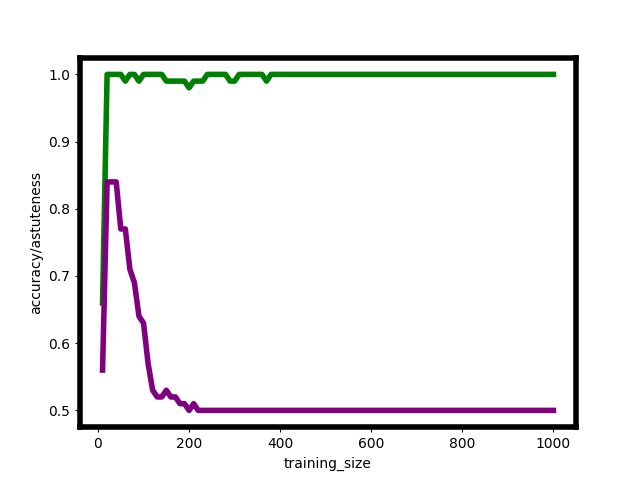
\includegraphics[width=.29\textwidth]{hist_noiseless_final}}\quad
%   \subfloat[][Noisy Histogram]{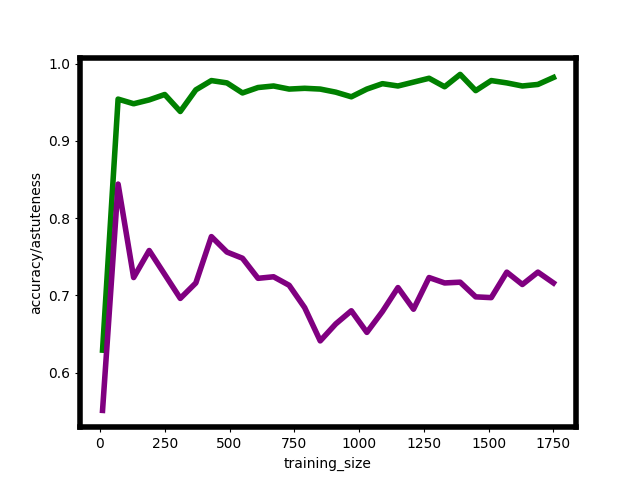
\includegraphics[width=.29\textwidth]{hist_noisy_final}} \quad
%   \subfloat[][Histogram trained on 500 samples]{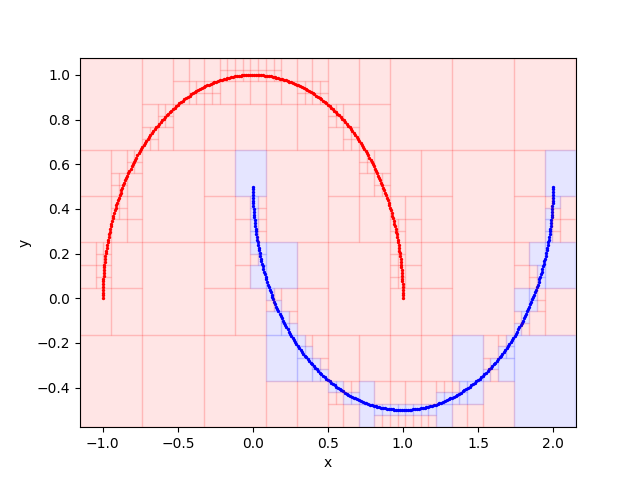
\includegraphics[width=.29\textwidth]{visual500}}\\
%   \subfloat[][Noiseless 1-NN]{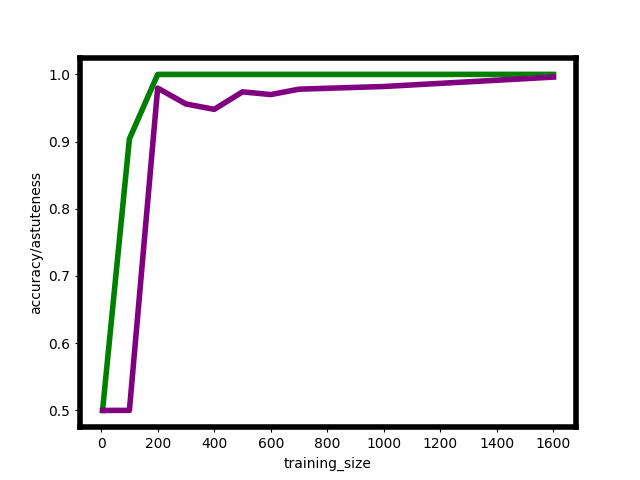
\includegraphics[width=.29\textwidth]{nn_noiseless_final}} \quad
%   \subfloat[][Noisy 1-NN]{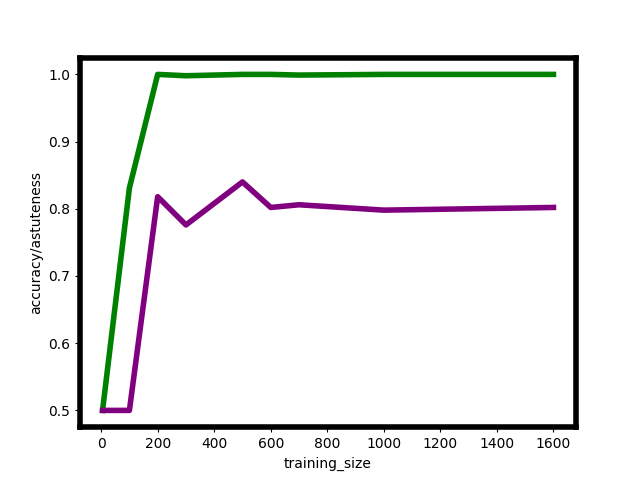
\includegraphics[width=.29\textwidth]{nn_noisy_final}}\quad
%   \subfloat[][Histogram trained on 3000 samples]{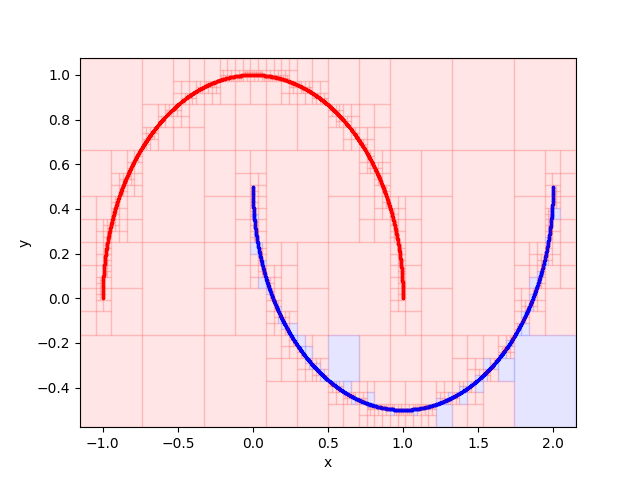
\includegraphics[width=.29\textwidth]{visual3000}}
%\end{center}
%\caption{Empirical accuracy/astuteness of different classifiers as a function of training sample size. Accuracy is shown in green, astuteness in purple. Left : Noiseless Setting. Right: Noisy Setting. Top Row: Histogram Classifier, Bottom Row: 1-Nearest Neighbor}
%\label{fig:1}
%\vskip -0.2in
%\end{figure}

\begin{figure}
\begin{subfigure}{0.31\textwidth}
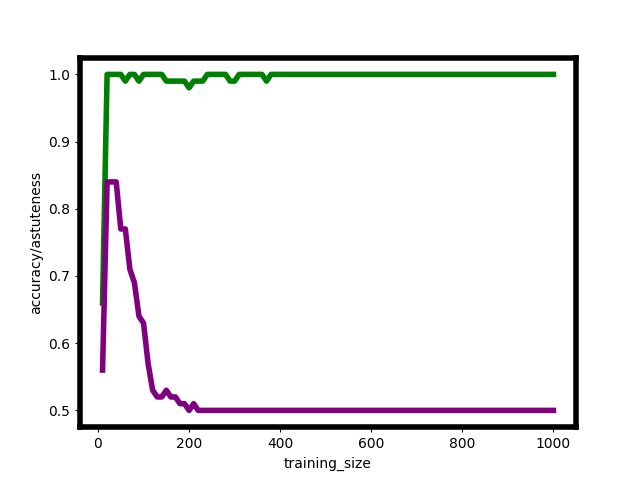
\includegraphics[width=\linewidth]{hist_noiseless_final}
%\caption{First subfigure} \label{fig:a}
\end{subfigure}\hspace*{\fill}
\begin{subfigure}{0.31\textwidth}
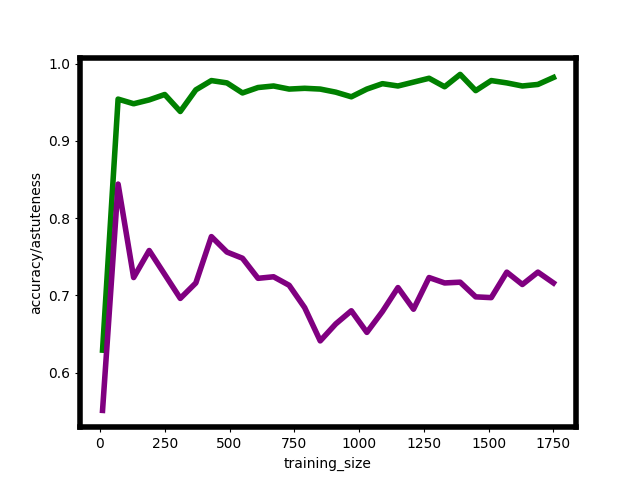
\includegraphics[width=\linewidth]{hist_noisy_final}
%\caption{Second subfigure} \label{fig:b}
\end{subfigure}\hspace*{\fill}
\begin{subfigure}{0.31\textwidth}
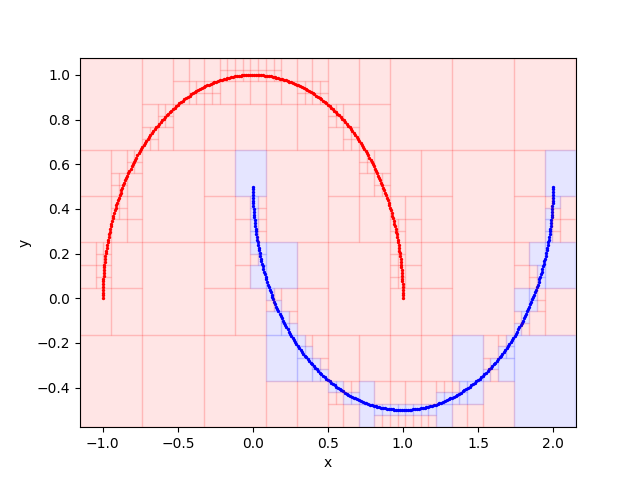
\includegraphics[width=\linewidth]{visual500}
%\caption{Fifth subfigure} \label{fig:e}
\end{subfigure}

\medskip
\begin{subfigure}{0.31\textwidth}
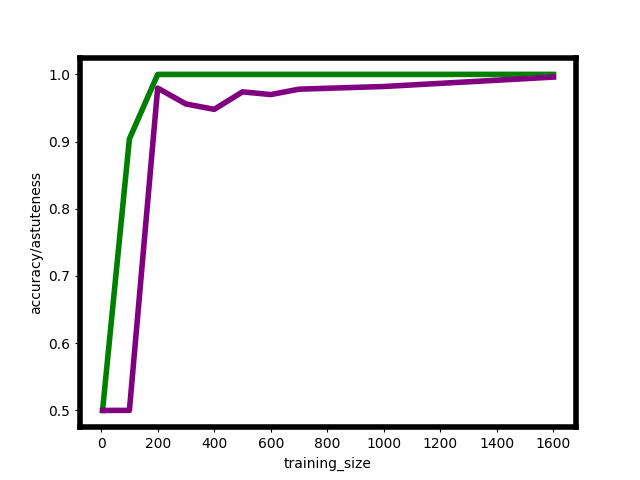
\includegraphics[width=\linewidth]{nn_noiseless_final}
%\caption{Third subfigure} \label{fig:c}
\end{subfigure}\hspace*{\fill}
\begin{subfigure}{0.31\textwidth}
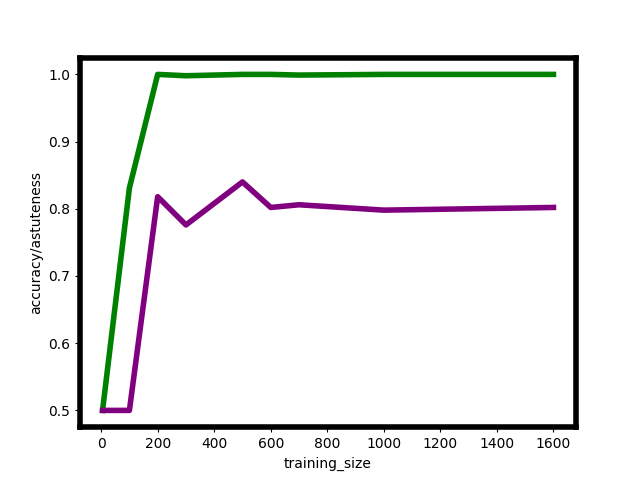
\includegraphics[width=\linewidth]{nn_noisy_final}
%\caption{Fourth subfigure} \label{fig:d}
\end{subfigure}\hspace*{\fill}
\begin{subfigure}{0.31\textwidth}
 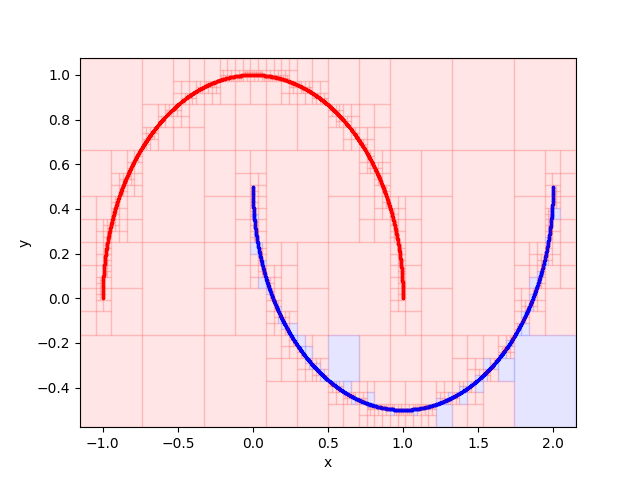
\includegraphics[width=\linewidth]{visual3000}
%\caption{Sixth subfigure} \label{fig:f}

\end{subfigure}

\caption{Empirical accuracy/astuteness of different classifiers as a function of training sample size. Accuracy is shown in green, astuteness in purple. Left : Noiseless Setting. Right: Noisy Setting. Top Row: Histogram Classifier, Bottom Row: 1-Nearest Neighbor} \label{fig:1}
\end{figure}

Our theoretical results are, by nature, large sample; we next validate how well they apply to the finite sample case by trying them out on a simple example. In particular, we ask the following question:

\begin{quote}
How does the robustness of non-parametric classifiers change with increasing sample size?
\end{quote}

This question is considered in the context of two simple non-parametric classifiers -- one nearest neighbor (which is guaranteed to be $r$-consistent) and histograms (which is not). To be able to measure performance with increasing data size, we look at a simple synthetic dataset -- the Half Moons. 

\subsection{Experimental Setup}

\paragraph{Classifiers and Dataset.} We consider two different classification algorithms -- one nearest neighbor (NN) and a Histogram Classifier (HC).  We use the Halfmoon dataset with two settings of the gaussian noise parameter $\sigma$, $\sigma = 0$ (Noiseless) and $\sigma =0.08$ (Noisy). For the Noiseless setting, observe that the data is already $0.1$-separated; for the Noisy setting, we use Adversarial Pruning (Algorithm~\ref{alg:gen}) with parameter $r = 0.1$ for both classification methods.

\paragraph{Performance Measure.} We evaluate robustness with respect to the $\ell_{\infty}$ metric, that is commonly used in the adversarial examples literature. Specifically, for each classifier, we calculate the {\em{empirical astuteness}}, which is the fraction of test examples on which it is astute.

Observe that computing the empirical astuteness of a classifier around an input $x$ amounts to finding the adversarial example that is {\em{closest to}} $x$ according to the $\ell_{\infty}$ norm. For the $1$-nearest neighbor, we do this using the optimal attack algorithm proposed by Yang et. al.~\cite{YRWC19}. For the histogram classifier, we use the optimal attack framework proposed by~\cite{YRWC19}, and show that the structure of the classifier can be exploited to solve the convex program efficiently. Details are in Appendix C.

We use an attack radius of $r = 0.1$ for the Noiseless setting, and $r = 0.09$ for the Noisy setting. For all classification algorithms, we plot the empirical astuteness as a function of the training set size. As a baseline, we also plot their standard accuracy on the test set. 

\subsection{Results}

The results are presented in Figure~\ref{fig:1}; the left two panels are for the Noiseless setting while the two center ones are for the Noisy setting.  

The results show that as predicted by our theory, for the Noiseless setting, the empirical astuteness of nearest neighbors converges to $1$ as the training set grows. For Histogram Classifiers, the astuteness converges to $0.5$ -- indicating that the classifier may grow less and less astute with higher sample size even for well-separated data. This is plausibly because the cell size induced by the histogram grows smaller with growing training data; thus, the classifier that outputs the default label $-1$ in empty cells is incorrect on adversarial examples that are close to a point with $+1$ label, but belongs to a different, empty cell. The rightmost panels in Figure~\ref{fig:1} provide a visual illustration of this process. 

For the Noisy setting, the empirical astuteness of adversarial pruning followed by nearest neighbors converges to $0.8$. For histograms with adversarial pruning, the astuteness converges to $0.7$, which is higher than the noiseless case but still clearly sub-optimal.

\subsection{Discussion}

Our results show that even though our theory is asymptotic, our predictions continue to be relevant in finite sample regimes. In particular, on well-separated data, nearest neighbors that we theoretically predict to be intrinsically robust is robust; histogram classifiers, which do not satisfy the conditions in Theorem~\ref{thm_stone_cons} are not. Our predictions continue to hold for data that is not well-separated. Nearest neighbors coupled with Adversarial
Pruning continues to be robust with growing sample size, while histograms continue to be non-robust. Thus our theory is confirmed by practice.

\section{Conclusion}

In conclusion, we rigorously analyze when non-parametric methods provide classifiers that are robust in the large sample limit. We provide a general condition that characterizes when non-parametric methods are robust on well-separated data, and show that Adversarial Pruning of~\cite{YRWC19} works on data that is not well-separated. 

Our results serve to provide a set of guidelines that can be used for designing non-parametric methods that are robust and accurate on well-separated data; additionally, we demonstrate that when data is not well-separated, preprocessing by adversarial pruning~\cite{YRWC19} does lead to optimally astute solutions in the large sample limit. 




%\input{chapters/chapter1/macros}
%\input{chapters/chapter1/introduction}
%\input{chapters/chapter1/related}
%\input{chapters/chapter1/definition}
%\input{chapters/chapter1/quantifying}
%\input{chapters/chapter1/visualizing}
%\input{chapters/chapter1/mitigation}
\graphicspath{{./chapters/chapter0/}}
\chapter{When are Non-Parametric Methods Robust?} 

\newtheorem{thm}{Theorem}
\newtheorem{lem}[thm]{Lemma}
\newtheorem{cor}[thm]{Corollary}

\newtheorem{defn}[thm]{Definition}
\newtheorem{ex}{Example}

\def\D{{\mathcal D}}
\def\X{\mathcal X}
\def\R{\mathbb R}
\def\Y{\{\pm 1\}}
\def\w{\hat{w}}
\def\P{\mathbb{P}}
\def\I{\hat{I}}
\def\b{g^*}
\def\r{\rho}
\def\rcons{r-consistent}
\def\rconsy{r-consistency}
\def\ap{AdvPrun}
\def\ga{RobustNonPar}

\section{Introduction}

Recent work has shown that many classifiers tend to be highly non-robust and that small strategic modifications to regular test inputs can cause them to misclassify~\cite{Szegedy14, Goodfellow14, MeekLowd05}. Motivated by the use of machine learning in safety-critical applications, this phenomenon has recently received considerable interest; however, what exactly causes this phenomenon -- known in the literature as {\em{adversarial examples}} -- still remains a mystery.

Prior work has looked at three plausible reasons why adversarial examples might exist. The first, of course, is the possibility that in real data distributions, different classes are very close together in space -- which does not seem plausible in practice. Another possibility is that classification algorithms may require more data to be robust than to be merely accurate; some prior work~\cite{Madry18, WJC18, Srebro19} suggests that this might be true for certain classifiers or algorithms. Finally, others~\cite{Bubeck19, Vinod19, WJC18} have suggested that better training algorithms may give rise to more robust classifiers -- and that in some cases, finding robust classifiers may even be computationally challenging.

In this work, we consider this problem in the context of general non-parametric classifiers. Contrary to parametrics, non-parametric methods are a form of local classifiers, and include a large number of pattern recognition methods such as nearest neighbors, decision trees, random forests and kernel classifiers. There is a richly developed statistical theory of non-parametric methods~\cite{devroye96}, which focuses on accuracy, and provides very general conditions under which these methods converge to the Bayes optimal with growing number of samples. We, in contrast, analyze robustness properties of these methods, and ask instead when they converge to the classifier with the highest astuteness at a desired radius $r$. Recall that the astuteness of a classifier at radius $r$ is the fraction of points from the distribution on which it is accurate and has the same prediction up to a distance $r$~\cite{WJC18, Madry18}.

 We begin by looking at the very simple case when data from different classes is well-separated -- by at least a distance $2r$. Although achieving astuteness in this case may appear trivial, we show that even in this highly favorable case, not all non-parametric methods provide robust classifiers -- and this even holds for methods that converge to the Bayes optimal in the large sample limit.  

This raises the natural question -- when do non-parametric methods produce astute classifiers? We next provide conditions under which a non-parametric method converges to the most astute classifier in the large sample limit under well-separated data. Our conditions are analogous to the classical conditions for convergence to the Bayes optimal~\cite{devroye96, Stone77}, but a little stronger. We show that nearest neighbors and kernel classifiers whose kernel functions decay fast enough, satisfy these conditions, and hence converge to astute classifiers in the large sample limit. In constrast, histogram classifiers, which do converge to the Bayes optimal in the large sample limit, may not converge to the most astute classifier. This indicates that there may be some non-parametric methods, such as nearest neighbors and kernel classifiers, that are more naturally robust when trained on well-separated data, and some that are not.

What happens when different classes in the data are not as well-separated? For this case, \cite{YRWC19} proposes a method called Adversarial Pruning that preprocesses the training data by retaining the maximal set of points such that different classes are distance $\geq 2r$ apart, and then trains a non-parametric method on the pruned data. We next prove that if a non-parametric method has certain properties, then the classifier produced by Adversarial Pruning followed by the method does converges to the most astute classifier in the large sample limit. We show that again nearest neighbors and kernel classifiers whose kernel functions decay faster than inverse polynomials satisfy these properties. Our results thus complement and build upon the empirical results of~\cite{YRWC19} by providing a performance guarantee. 

What can we conclude about the cause for adversarial examples? Our results seem to indicate that at least for non-parametrics, it is mostly the training algorithms that are responsible. With a few exceptions, decades of prior work in machine learning and pattern recognition has largely focussed on designing training methods that provide increasingly accurate classifiers -- perhaps to the detriment of other aspects such as robustness. In this context, our results serve to (a) provide a set of guidelines that can be used for designing non-parametric methods that are robust and accurate on well-separated data and (b) demonstrate that when data is not well-separated, preprocessing through adversarial pruning~\cite{YRWC19} may be used to ensure convergence to optimally astute solutions in the large sample limit. 

\subsection{Related Work}

There is a large body of work on adversarial attacks~\cite{Carlini17, Liu17, Papernot17, Papernot16,Szegedy14} and defenses~\cite{Hein17,Katz17,Schmidt18,Wu16,Steinhardt18, Sinha18} in the parametric setting, specifically focusing on neural networks. On the other hand, adversarial examples for nonparametric classifiers have mostly been studied in a much more ad-hoc manner, and to our knowledge, there has been no theoretical investigation into general properties of algorithms that promote robustness in non-parametric classifiers.

For nearest neighbors, there has been some prior work on adversarial attacks~\cite{Amsaleg17, Sitawarin19, WJC18, YRWC19} as well as defenses. Wang et. al. \cite{WJC18} proposes a defense for 1-NN by pruning the input sample. However, their defense learns a classifier whose robustness regions converge towards those of the Bayes optimal classifier, which itself may potentially have poor robustness properties. Yang et. al. \cite{YRWC19} accounts for this problem by proposing the notion of the $r$-optimal classifier, and propose an algorithm called Adversarial Pruning which can be interpreted as a finite sample approximation to the $r$-optimal. However, they do not provide formal performance guarantees for Adversarial Pruning, which we do. 

For Kernel methods, Hein and Andriushchenko \cite{Hein17} study lower bounds on the norm of the adversarial manipulation that is required for changing a classifiers output. They specifically study bounds for Kernel Classifiers, and propose an empirically based regularization idea that improves robustness. In this work, we improve the robustness properties of kernel classification through adversarial pruning, and show formal guarantees regarding convergence towards the $r$-optimal classifier. 

For decision trees and random forests, attacks and defenses have been provided by \cite{Hein19, Kantchelian15, Hsiehicml19}. Again, most of the work here is empirical in nature, and convergence guarantees are not provided. 

Pruning has a long history of being applied for improving nearest neighbors \cite{Gates72, Gottlieb14, Hart68, KontorovichSW17, KontorovichW15, Hanneke19}, but this has been entirely done in the context of generalization, without accounting for robustness. In their work, Yang et. al. empirically show that adversarial pruning can improve robustness for nearest neighbor classifiers. However, they do not provide any formal guarantees for their algorithms. In this work, we prove formal guarantees for \textit{adversarial pruning} in the large sample limit, both for nearest neighbors as well as for more general \textit{weight functions.} 

There is a long history of literature for understanding the consistency of Kernel classifiers \cite{Steinwart05, Stone77}, but this has only been done for accuracy and generalization. In this work, we find different conditions are needed to ensure that a Kernel classifier converges in robustness in addition to accuracy.

\section{Preliminaries}

\subsection{Setting}
We consider binary classification where instances are drawn from a totally bounded metric space $\X$ that is equipped with distance metric denoted by $d$, and the label space is $\Y = \{ -1, +1 \}$. The classical goal of classification is to build a highly \textit{accurate} classifier, which we define as follows.

\begin{defn}
(Accuracy) Let $\D$ be a distribution over $\X \times \Y$, and let $f \in \Y^\X$ be a classifier. Then the \textbf{accuracy} of $f$ over $\D$, denoted $A(f, \D)$, is the fraction of examples $(x,y) \sim \D$ for which $f(x) = y$. Thus $$A(f, \D) = P_{(x,y) \sim \D}[f(x) = y].$$
\end{defn}

In this work, we consider \textit{robustness} in addition to accuracy. Let $B(x,r)$ denoted the closed ball of radius $r$ centered at $x$. 

\begin{defn}
(Robustness) A classifier $f \in \Y^\X$ is said to be \textbf{robust} at $x$ with radius $r$ if $f(x) = f(x')$ for all $x' \in B(x,r)$.
\end{defn}

Our goal is to find non-parametric algorithms that output classifiers that are robust, in addition to being accurate. To account for both criteria, we combine them into a notion of \textit{astuteness}~\cite{WJC18, Madry18}. 

\begin{defn}
(Astuteness) A classifier $f \in \Y^\X$ is said to be \textbf{astute} at $(x,y)$ with radius $r$ if $f$ is robust at $x$ with radius $r$ and $f(x) = y$. The \textbf{astuteness} of $f$ over $\D$, denoted $A_r(f, \D)$, is the fraction of examples $(x,y) \sim \D$ for which $f$ is astute at $(x,y)$ with radius $r$. Thus $$A_r(f, \D) = P_{(x, y) \sim \D}[f(x') = y, \forall x' \in B(x,r)].$$
\end{defn}

It is worth noting that $A_0(f, \D) = A(f, \D)$, since astuteness with radius $0$ is simply the accuracy. For this reason, we will use $A_0(f, \D)$ to denote accuracy from this point forwards.

\subsection{Notions of Consistency}

Traditionally, a classification algorithm is said to be consistent if as the sample size grows to infinity, the accuracy of the classifier it learns converges towards the best possible accuracy on the underlying data distribution. We next introduce and formalize an alternative form of consistency, called $r$-consistency, that applies to robust classifiers.

We begin with a formal definition of the Bayes Optimal Classifier -- the most accurate classifier on a distribution -- and consistency. 

\begin{defn}
(Bayes Optimal Classifier) The \textbf{Bayes Optimal Classifier} on a distribution $\D$, denoted by $\b$, is defined as follows. Let $\eta(x) = p_\D(+1|x)$. Then
 \[ \b(x) = \begin{cases} 
      +1 & \eta(x) \geq 0.5 \\
      -1 & \eta(x) < 0.5 \\
   \end{cases}
\]
It can be shown that $\b$ achieves the highest accuracy over $\D$ over all classifiers.
\end{defn}

\begin{defn}
(Consistency) Let $M$ be a classification algorithm  over $\X \times \Y$. $M$ is said to be \textbf{consistent} if for any $\D$ over $\X \times \Y$, and any $\epsilon, \delta$ over $(0,1)$, there exists $N$ such that for $n \geq N$, with probability $1-\delta$ over $S \sim \D^n$, we have: $$A(M(S), \D) \geq A(\b, \D) - \epsilon,$$ where $\b$ is the Bayes optimal classifier for $\D$. 
\end{defn}

How can we incorporate robustness in addition to accuracy in this notion? A plausible way, as used in~\cite{WJC18}, is that the classifier should converge towards being astute where the Bayes Optimal classifier is astute. However, the Bayes Optimal classifier is not necessarily the most astute classifier and may even have poor astuteness. To see this, consider the following example. 

\paragraph{Example 1}
Consider $\D$ over $\X = [0,1]$ such that $\D_\X$ is the uniform distribution and $$p(y=1|x) = \frac{1}{2} + \sin \frac{4 \pi x}{r}.$$ For any point $x$, there exists $x_1, x_2 \in ([x-r, x+r] \cap [0,1])$ such that $p(y=1|x_1) > \frac{1}{2}$ and $p(y=1|x_2) < \frac{1}{2}$. $A_r(\b, r) = 0$. However, the classifier that always predicts $f(x) = +1$ does better. It is robust everywhere, and since $P_{(x,y) \sim \D}[y = +1] = \frac{1}{2}$, it follows that $A_r(f, \D) = \frac{1}{2}$. \\ \\

This motivates the notion of the $r$-optimal classifier, introduced by~\cite{YRWC19}, which is the classifier with maximum astuteness. 

\begin{defn}
($r$-optimal classifier) The \textbf{$r$-optimal classifier} of a distribution $G$ denoted by $\b_r$ is the classifier with maximum astuteness. Thus $$\b_r = \argmax_{f \in \Y^\X} A_r(f, \D).$$ We let $A_r^*(\D)$ denote $A_r(\b_r, \D)$. 
\end{defn}

Observe that $\b_r$ is not necessarily unique. To account for this, we use $A_r^*(\D)$ in our definition for \rconsy. 

\begin{defn} \label{defn_archons}
(\rcons) Let $M$ be a classification algorithm over $\X \times \Y$. $M$ is said to be \textbf{\rcons} if for any $\D$,  any $\epsilon, \delta \in (0,1)$, and $0 < \gamma < r$, there exists $N$ such that for $n \geq N$, with probability $1-\delta$ over $S \sim \D^n$, $$A_{r-\gamma}(M(S), \D) \geq A_r^*(\D) - \epsilon.$$ if the above conditions hold for a specific distribution $\D$, we say that $M$ is \rcons\emph{ }with respect to $\D$. 
\end{defn}

Observe that in addition to the usual $\epsilon$ and $\delta$, there is an extra parameter $\gamma$ which measures the gap in the robustness radius. We may need this parameter as when classes are exactly $2r$ apart, we may not be able to find the exact robust boundary with only finite samples. 

Our analysis will be centered around understanding what kinds of algorithms $M$ provide highly astute classifiers for a given radius $r$. We begin by first considering the special case of \textit{$r$-separated} distributions. 

\begin{defn}
($r$-separated distributions) A distribution $\D$ is said to be \textbf{$r$-separated} if there exist subsets $T^+, T^- \subset \X$ such that 
\begin{enumerate}
	\item $\P_{(x,y) \sim \D}[x \in T^y] = 1$. 
	\item $\forall x_1 \in T^+, \forall x_2 \in T^-$, $d(x_1, x_2) > 2r$.
\end{enumerate}
\end{defn}

Observe that if $\D$ is $r$-separated, $A_r(\b_r, \D) = 1$.

\subsection{Non-parametric Classifiers}\label{classifiers}

Many non-parametric algorithms classify points by averaging labels over a local neighborhood from their training data. A very general form of this idea is encapsulated in \textit{weight functions} -- which is the general form we will use.

\begin{defn} \label{def:weight}
\cite{devroye96} A \textbf{weight function} $W$ is a non-parametric classifier with the following properties.
\begin{enumerate}
	\item Given input $S = \{(x_1, y_1), (x_2, y_2,), \dots, (x_n, y_n)\} \sim \D^n$, $W$ constructs functions $w_1^S, \dots, w_n^S: \X \to [0, 1]$ such that for all $x \in \X$, $\sum_1^n w_i^S(x) = 1$. The functions $w_i^S$ are allowed to depend on $x_1, x_2, \dots x_n$ but must be independent of $y_1, y_2, \dots, y_n$. 
	\item $W$ has output $W_S$ defined as \[ W_S(x) = \begin{cases} 
      +1 & \sum_1^n w_i^S(x)y_i > 0 \\
      -1 & \sum_1^n w_i^S(x)y_i \leq 0 \\
   \end{cases}
\]
As a result, $w_i^S(x)$ can be thought of as the weight that $(x_i, y_i)$ has in classifying $x$.
\end{enumerate}
\end{defn}

Weight functions encompass a fairly extensive set of common non-parametric classifiers, which is the motivation for considering them. We now define several common non-parametric algorithms that can be construed as weight functions. 

\begin{defn}
A \textbf{histogram classifier}, $H$, is a non-parametric classification algorithm over $\R^d \times \Y$ that works as follows. For a distribution $\D$ over $\R \times \Y$, $H$ takes $S = \{(x_i, y_i): 1 \leq i \leq n\} \sim \D^n$ as input. Let $k_i$ be a sequence with $\lim_{i \to \infty} k_i = \infty$ and $\lim_{i \to \infty} \frac{k_i}{i} = 0$. $H$ constructs a set of hypercubes $C = \{c_1, c_2, \dots, c_m\}$ as follows:
\begin{enumerate}
	\item Initially $C = \{c\}$, where $S \subset c$.
	\item For $c \in C$, if $c$ contains more than $k_n$ points of $S$, then partition $c$ into $2^d$ equally sized hypercubes, and insert them into $C$.
	\item Repeat step $2$ until all cubes in $C$ have at most $k_n$ points. 
\end{enumerate}
For $x \in \R$ let $c(x)$ denote the unique cell in $C$ containing $x$. If $c(x)$ doesn't exist, then $H_S(x) = -1$ by default. Otherwise, \[ H_S(x) = \begin{cases} 
      +1 & \sum_{x_i \in c(x)} y_i > 0 \\
      -1 & \sum_{x_i \in c(x)}y_i \leq 0 \\
   \end{cases}.
\]
\end{defn}

Histogram classifiers are weight functions in which all $x_i$ contained within the same cell as $x$ are given the same weight $w_i^S(x)$ in predicting $x$, while all other $x_i$ are given weight $0$. 

\begin{defn}
A \textbf{kernel classifier} is a weight function $W$ over $\X \times \Y$ constructed from function $K: \R^+ \cup \{0\} \to \R^+$ and some sequence $\{h_n\} \subset \R^+$ in the following manner. Given $S = \{(x_i, y_i)\} \sim \D^n$, we have $$w_i^S(x) = \frac{K(\frac{d(x, x_i)}{h_n})}{\sum_{j = 1}^n K(\frac{d(x, x_j)}{h_n})}.$$ Then, as above, $W$ has output \[ W_S(x) = \begin{cases} 
      +1 & \sum_1^n w_i^S(x)y_i > 0 \\
      -1 & \sum_1^n w_i^S(x)y_i \leq 0 \\
   \end{cases}
\]
\end{defn}

Finally, we note that $k_n$-nearest neighbors is also a weight function; $w_i^S(x) = \frac{1}{k_n}$ if $x_i$ is one of the $k_n$ closest neighbors of $x$ and $0$ otherwise.

\section{Warm Up: $r$-separated distributions}

We begin by considering the case when the data distribution is $r$-separated; the more general case is considered in Section~\ref{sec:general}. While classifying $r$-separated distributions robustly may appear almost trivial, learning an arbitrary classifier does not necessarily produce an astute result. To see this, consider the following example of a histogram classifier -- which is known to be consistent. 


We let $H$ denote the histogram classifier over $\R$.

\paragraph{Example 2}
Consider the data distribution $\D = \D^+ \cup \D^-$ where $D^+$ is the uniform distribution over $[0, \frac{1}{4})$ and $D^-$ is the uniform distribution over $(\frac{1}{2}, 1]$, $p(+1|x) = 1$ for $x \in \D^+$, and $p(-1|x) = 1$ for $x \in \D^-$. 

We make the following observations (refer to Figure \ref{fig:histogram}).
\begin{enumerate}
	\item $\D$ is $0.1$-separated, since the supports of $\D^+$ and $\D^-$ have distance $0.25 > 0.2$. 
	\item If $n$ is sufficiently large, $H$ will construct the cell $[0.25, 0.5)$, which will not be split because it will never contain any points. 
	\item $H_S(x) = -1$ for $x \in [0.25, 0.5)$.
	\item $H_S$ is not astute at $(x,1)$ for $x \in (0.15, 0.25)$. Thus $A_{0.1}(H_S, \D) = 0.8$.
\end{enumerate}

\begin{figure}
\centering
\definecolor{dtsfsf}{rgb}{0.8274509803921568,0.1843137254901961,0.1843137254901961}
\definecolor{sexdts}{rgb}{0.1803921568627451,0.49019607843137253,0.19607843137254902}
\begin{tikzpicture}[line cap=round,line join=round,>=triangle 45,x=1cm,y=1cm]
\clip(-4.68,0) rectangle (2.46,3);
\draw [line width=2pt] (-3.8971542001619626,1.7601524817792173)-- (-3.90319974718047,1.0800284421971598);
\draw [line width=2pt] (-2.7721542001619626,1.7501524817792171)-- (-2.7781997471804694,1.0700284421971598);
\draw [line width=2pt] (-1.6471542001619623,1.7401524817792173)-- (-1.6531997471804694,1.0600284421971597);
\draw [line width=2pt] (0.6028457998380374,1.720152481779217)-- (0.5968002528195302,1.0400284421971597);
\draw [line width=2pt] (-2.775,1.43)-- (-1.65,1.42);
\draw [line width=2pt,color=sexdts] (-1.65,1.42)-- (0.6,1.4);
\draw [line width=2pt,color=sexdts] (-3.9,1.44)-- (-3.2002330680045032,1.4337798494933733);
\draw [line width=2pt,color=dtsfsf] (-3.2002330680045032,1.4337798494933733)-- (-2.775,1.43);
\draw (-3.54,2.48) node[anchor=north west] {$\mathcal{D}^+$};
\draw (-0.76,2.46) node[anchor=north west] {$\mathcal{D}^-$};
\draw (-4,1.1) node[anchor=north west] {0};
\draw (-3.14,1.08) node[anchor=north west] {0.25};
\draw (-1.86,1.1) node[anchor=north west] {0.5};
\draw (0.5,1.08) node[anchor=north west] {1};
\end{tikzpicture}
\caption{$H_S$ is astute in the green region, but not robust in the red region.} \label{fig:histogram}
\end{figure}

Example 2 shows that histogram classifiers do not always learn astute classifiers even when run on $r$-separated distributions. This motivates the question: which non-parametric classifiers do?

We answer this question in the following theorem, which gives sufficient conditions for a weight function (definition \ref{def:weight}) to be $r$-consistent over an $r$-separated distribution.

\begin{thm}\label{thm_stone_cons}
Let $\D$ be a distribution over $\X \times \Y$, and let $W$ be a weight function. Let $X$ be a random variable with distribution $\D_\X$, and $S = \{(x_1, y_1), (x_2, y_2), \dots, (x_n, y_n)\} \sim \D^n$. Suppose that for any $0 < a < b,$ $$\lim_{n \to \infty} \mathbb{E}_{X, S} \big [ \sup_{x' \in B(X, a)} \sum_1^n w_i^S(x')I_{||x_i - x'|| > b} \big] = 0.$$  Then if $\D$ is $r$-separated, $W$ is \rcons\emph{ } with respect to $\D$.  
\end{thm}

First, we compare Theorem \ref{thm_stone_cons} to Stone's theorem \cite{Stone77}, which gives sufficient conditions for a weight function to be consistent (i.e. converge in accuracy towards the Bayes optimal). For convenience, we include a statement of Stone's theorem. 
\begin{thm}\label{thm_stone}
\cite{Stone77} Let $W$ be weight function over $\X \times \Y$. Suppose the following conditions hold for any distribution $\D$ over $\X \times \Y$.  Let $X$ be a random variable with distribution $\D_\X$, and $S = \{(x_1, y_1), (x_2, y_2), \dots, (x_n, y_n)\} \sim \D^n$. All expectations are taken over $X$ and $S$. 
\begin{enumerate}
	\item There is a constant $c$ such that, for every nonnegative measurable function $f$ satisfying $\mathbb{E} [f(X)] < \infty$, $$\mathbb{E} [\sum_1^n w_i^S(X)f(x_i)] \leq c \mathbb{E} [f(x)].$$
	\item For all $a > 0$, $$\lim_{n \to \infty} \mathbb{E}[\sum_1^n w_i^S(x)I_{||x_i - X|| > a}] = 0,$$ where $I_{||x_i - X|| > a}$ is an indicator variable. 
	\item $$\lim_{n \to \infty} \mathbb{E}[\max_{1 \leq i \leq n} w_i^S(X)] = 0.$$
\end{enumerate}
Then $W$ is consistent. 
\end{thm}
There are two main differences between Theorem \ref{thm_stone_cons} and Stone's theorem.
 \begin{enumerate}
 	\item Conditions 1. and 3. of Stone's theorem are no longer necessary. This is because $r$-separated distributions are well-separated and thus have simpler conditions for consistency. In fact, a slight modification of the arguments of~\cite{Stone77} shows that for $r$-separated distributions, condition 2. alone is sufficient for consistency.
 	\item Condition 2. is strengthened. Instead of requiring the weight of $x_i$'s outside of a given radius to go to $0$ for $X \sim \D$, we require the same to \textit{uniformly} hold over a ball centered at $X$. 
\end{enumerate}  
 


Theorem \ref{thm_stone_cons} provides a general condition that allows us to verify the $r$-consistency of non-parametric methods. We now show below that two common non-parametric algorithms -- $k_n$-nearest neighbors and kernel classifiers with rapidly decaying kernel functions -- satisfy the conditions of Theorem~\ref{thm_stone_cons}.
 
\begin{cor}\label{nn_sep_thm}
Let $\D$ be any $r$-separated distribution. Let $k_n$ be any sequence such that $\lim_{n \to \infty} \frac{k_n}{n} = 0$, and let $M$ be the $k_n$-nearest neighbors classifier on a sample $S \sim \D^n$. Then $M$ is \rcons\emph{ }with respect to $\D$. 
\end{cor}

\paragraph{\textbf{Remarks:}}
\begin{enumerate}
	\item Because the data distribution is $r$-separated, $k_n = 1$ will be $r$-consistent. Also observe that for $r$-separated distributions, $k_n = 1$ will converge towards the Bayes Optimal classifier.
	\item In general, $M$ converges towards the Bayes Optimal classifier provided that $k_n \to \infty$ in addition to $k_n /n \to 0$. This condition is not necessary for \rconsy -- because the distribution is $r$-separated. 
\end{enumerate}



We next show that kernel classifiers are also $r$-consistent on $r$-separated data distributions, provided the kernel function decreases rapidly enough. 

\begin{cor}\label{thm_kernel}
Let $W$ be a kernel classifier over $\X \times \Y$ constructed from $K$ and $h_n$. Suppose the following properties hold for $K$ and $h_n$.
\begin{enumerate}
	\item For any $c > 1$, $\lim_{x \to \infty} \frac{K(cx)}{K(x)} = 0.$
	\item $\lim_{n \to \infty} h_n = 0.$
\end{enumerate}
If $\D$ is an $r$-separated distribution over $\X \times \Y$, then $W$ is \rcons\emph{ }with respect to $\D$. 
\end{cor}

Observe that Condition 1. is satisfied for any $K(x)$ that decreases more rapidly than an inverse polynomial -- and is hence satisfied by most popular kernels like the Gaussian kernel. Is the condition on $K$ in Corollary~\ref{thm_kernel} necessary? The following example illustrates that a kernel classifier with any arbitrary $K$ is not necessarily $r$-consistent. This indicates that some sort of condition needs to be imposed on $K$ to ensure $r$-consistency; finding a tight necessary condition however is left for future work. 

 \paragraph{Example 3} Let $\X = [-1, 1]$ and let $\D$ be a distribution with $p_\D(-1, -1) = 0.1$ and $p_\D(1, 1) = 0.9$. Clearly, $\D$ is $0.3$-separated. Let $K(x) = e^{-\min(|x|, 0.2)^2}$. Let $h_n$ be any sequence with $\lim_{n \to \infty} h_n = 0$ and $\lim_{n \to \infty} nh_n = \infty$. Let $W$ be the weight classifier with input $S = \{(x_1, y_1), (x_2, y_2), \dots, (x_n, y_n)\}$ such that $$w_i^S(x) = \frac{K(\frac{|x- x_i|}{h_n})}{\sum_{j=1}^n K(\frac{|x-x_j|}{h_n})}.$$ $W$ can be shown to satisfy all the conditions of Theorem \ref{thm_stone} (the proof is analogous to the case for a Gaussian Classifier), and is therefore consistent. However, $W$ does not learn a robust classifier on $\D$ for $r = 0.3$. 

Consider $x = -0.7$. For any $\{(x_1, y_1), (x_2, y_2), \dots, (x_n, y_n)\} \sim \D^n$, all $x_i$ will either be $-1$ or $1$. Therefore, since $K(|x - (-1)|) = K(|x - 1|)$, it follows that $w_i^S(x) = \frac{1}{n}$ for all $1 \leq i \leq n$. Since $x_i = 1$ with probability $0.9$, it follows that with high probability $x$ will be classified as $1$ which means that $f$, the output of $W$, is not robust at $x = -1$. Thus $f$ has astuteness at most $0.9$ which means that $W$ is \textit{not} \rcons\ for $r=0.3$. 

\section{General Distributions}\label{sec:general}


We next consider more general data distributions, where data from different classes may be close together in space, and may even overlap. Observe that unlike the $r$-separated case, here there may be no classifier with astuteness one. Thus, a natural question is: what does the optimally astute classifier look like, and how can we build non-parametric classifiers to this limit?

\subsection{The $r$-Optimal Classifier and Adversarial Pruning}

\cite{YRWC19} propose a large-sample limit -- called the $r$-optimal -- and show that it is analogous to the Bayes Optimal classifier for robustness. More specifically, given a data distribution $D$, to find the $r$-optimal classifier, we solve the following optimization problem.  

\begin{equation}\label{optim_prob}
\begin{split}
\max_{S_{+1}, S_{-1}} &\int_{x \in S_{+1}} p(y=+1|x)d\mu_{\D}(x) + \\
&\int_{x \in S_{-1}} p(y=-1|x)d\mu_{\D}(x) \\
&\text{ subject to } d(S_{+1}, S_{-1}) > 2r 
\end{split}
\end{equation}

Then, the $r$-optimal classifier is defined as follows. 

\begin{defn}
\cite{YRWC19} Fix $r, \D$. Let $S_{+1}^*$ and $S_{-1}^*$ be any optimizers of (\ref{optim_prob}). Then the $r$-optimal classifier, $\b_r$ is any classifier such that $\b_r(x) = j$ whenever $d(S_j^*, x) \leq r$. 
\end{defn}

\cite{YRWC19} show that the $r$-optimal classifier achieves the optimal astuteness -- out of all classifiers on the data distribution $\D$; hence, it is a robustness analogue to the Bayes Optimal Classifier. Therefore, for general distributions, the goal in robust classification is to find non-parametric algorithms that output classifiers that converge towards $\b_r$. 

To find robust classifiers, \cite{YRWC19} propose Adversarial Pruning -- a defense method that preprocesses the training data by making it better separated. More specifically, Adversarial Pruning takes as input a training dataset $S$ and a radius $r$, and finds the largest subset of the training set where differently labeled points are at least distance $2r$ apart. 


\begin{defn}
A set $S_r \subset \X \times \Y$ is said to be \textbf{$r$-separated} if for all $(x_1, y_1), (x_2, y_2) \in S_r$, if $y_1 \neq y_2$, then $d(x_1, x_2) > 2r$. To \textbf{adversarially prune} a set $S$ is to return its largest $r$-separated subset. We let $\ap(S, r)$ denote the result of adversarially pruning $S$.  
\end{defn}

Once an $r$-separated subset $S_r$ of the training set is found, a standard non-parametric method is trained on $S_r$.  While~\cite{YRWC19} show good empirical performance of such algorithms, no formal guarantees are provided. We next formally characterize when adversarial pruning followed by a non-parametric method results in a classifier that is provably $r$-consistent.

Specifically, we consider analyzing the general algorithm provided in Algorithm \ref{alg:gen}.

%\begin{algorithm}[tb]
%   \caption{\ga}
%   \label{alg:gen}
%\begin{algorithmic}
%   \STATE {\bfseries Input:} $S \sim \D^n$, weight function $W$, 
%   robustness radius $r$
%   \STATE $S_r \leftarrow \ap(S, r)$
%   \STATE{\bfseries Output:} $W_{S_r}$
%\end{algorithmic}
%\end{algorithm}

\begin{algorithm}[H]
    \SetAlgoLined
    {\bfseries Input:} $S \sim \D^n$, weight function $W$, robustness radius $r$\;
    
    $S_r \leftarrow \ap(S, r)$\;
    
    {\bfseries Output:} $W_{S_r}$\;
    

\caption{\ga}\label{alg:gen}
\end{algorithm}

\subsection{Convergence Guarantees}

We begin with some notation. For any weight function $W$ and radius $r > 0$, we let $\ga(W,r)$ represent the weight function that outputs weights for $S \sim \D^n$ according to $\ga(S, W, r)$. In particular, this can be used to convert any weight function algorithm into a new weight function which takes robustness into account. A natural question is, for which weight functions $W$ is $\ga(W,r)$ \rcons? Our next theorem provides sufficient conditions for this.

\begin{thm}\label{thm_weight_general}
Let $W$ be a weight function over $\X \times \Y$, and let $\D$ be a distribution over $\X \times \Y$. Fix $r >0$. Let $S_r = \ap(S, r)$.  For convenience, relabel $x_i, y_i$ so that $S_r = \{(x_1, y_1), (x_2, y_2), \dots, (x_m, y_m)\}$. Suppose that for any $0 < a < b,$ 
\begin{equation*}\label{condition}
\lim_{n \to \infty} \mathbb{E}_{S \sim \D^n}\big [ \frac{1}{m} \sum_{i = 1}^m \sup_{x \in B(x_i, a)} \sum_{j = 1}^m w_j^{S_r}(x)I_{||x_j - x|| > b} \big] = 0. 
\end{equation*}
Then $\ga(W,r)$ is \rcons\emph{ }with respect to $\D$. 
\end{thm}

\paragraph{\textbf{Remark}:}
There are two important differences between the conditions in Theorem \ref{thm_weight_general} and Theorem~\ref{thm_stone_cons}.
\begin{enumerate}
	\item We replace $S$ with $S_r$.
	\item The expectation over $X \sim \D_\X$ is replaced with an average over $\{x_1, x_2, \dots, x_m\}$. The intuition here is that we are replacing $\D$ with a uniform distribution over $S_r$. While $\D$ may not be $r$-separated, the uniform distribution over $S_r$ is, and represents the region of points where our classifier is astute. 
\end{enumerate}

A natural question is what satisfies the conditions in Theorem~\ref{thm_weight_general}. We next show that $k_n$-nearest neighbors and kernel classifiers with rapidly decaying kernel functions continue to satisfy the conditions in Theorem \ref{thm_weight_general}; this means that these classifiers, when combined with Adversarial Pruning, will converge to $r$-optimal classifiers in the large sample limit.

\begin{cor}\label{thm_NN_gen}
Let $k_n$ be a sequence with $\lim_{n \to \infty} \frac{k_n}{n} = 0$, and let $M$ denote the $k_n$-nearest neighbor algorithm. Then for any $r > 0$, $\ga(M, r)$ is \rcons.
\end{cor}
\paragraph{\textbf{Remark}:} Corollary \ref{thm_NN_gen} gives a formal guarantee in the large sample limit for the modified nearest-neighbor algorithm proposed by \cite{YRWC19}.

\begin{cor}\label{thm_kern_gen}
Let $W$ be a kernel classifier over $\X \times \Y$ constructed from $K$ and $h_n$. Suppose the following properties hold for $K$ and $h_n$.
\begin{enumerate}
	\item For any $c > 1$, $\lim_{x \to \infty} \frac{K(cx)}{K(x)} = 0.$
	\item $\lim_{n \to \infty} h_n = 0.$
\end{enumerate}
Then for any $r > 0$, $\ga(W, r)$ is \rcons.
\end{cor}

Observe again that Condition 1. is satisfied by any $K$ that decreases more rapidly than an inverse polynomial kernel; it is thus satisfied by most popular kernels, such as the Gaussian kernel. 

\section{Validation}
%\begin{figure}[ht]
%\vskip 0.2in
%\begin{center}
%\subfloat[][Noiseless Histogram]{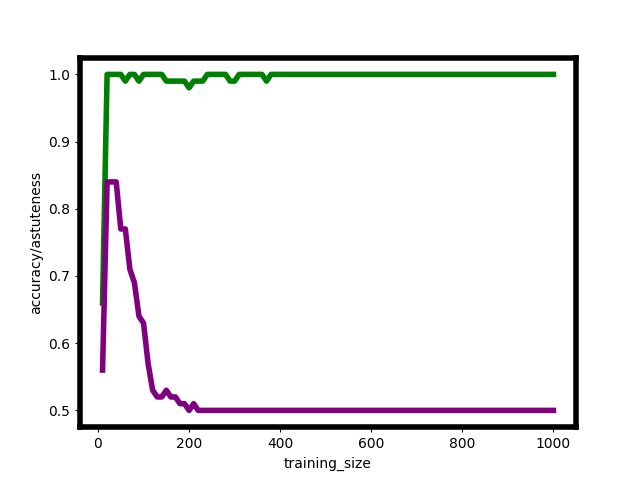
\includegraphics[width=.29\textwidth]{hist_noiseless_final}}\quad
%   \subfloat[][Noisy Histogram]{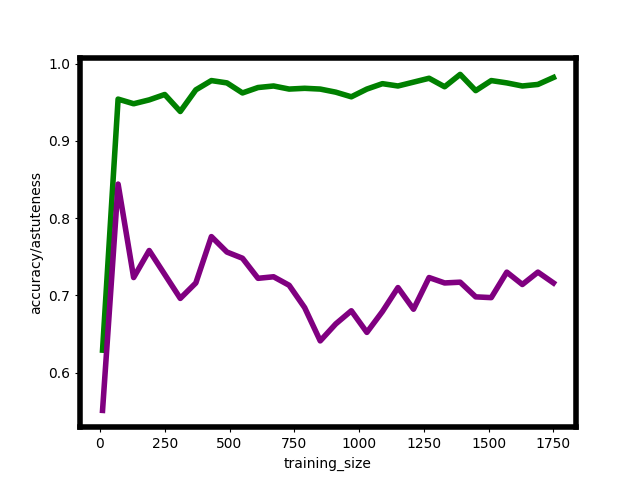
\includegraphics[width=.29\textwidth]{hist_noisy_final}} \quad
%   \subfloat[][Histogram trained on 500 samples]{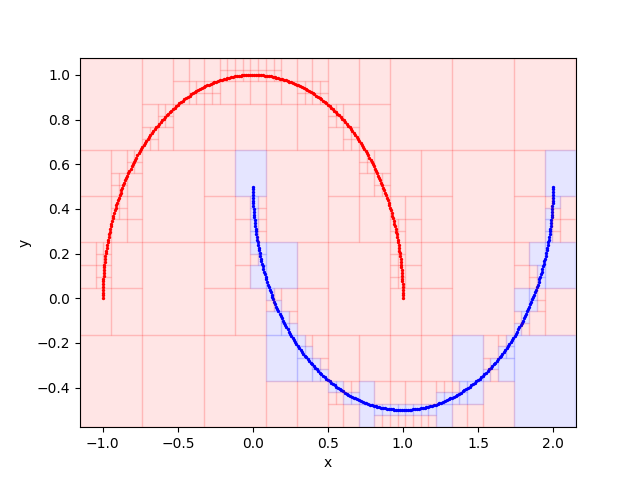
\includegraphics[width=.29\textwidth]{visual500}}\\
%   \subfloat[][Noiseless 1-NN]{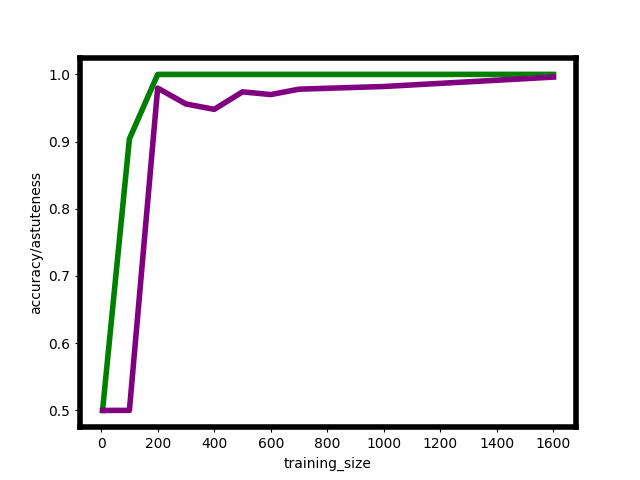
\includegraphics[width=.29\textwidth]{nn_noiseless_final}} \quad
%   \subfloat[][Noisy 1-NN]{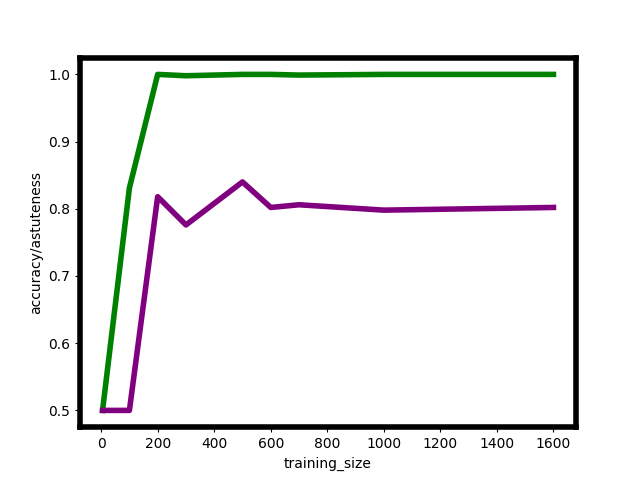
\includegraphics[width=.29\textwidth]{nn_noisy_final}}\quad
%   \subfloat[][Histogram trained on 3000 samples]{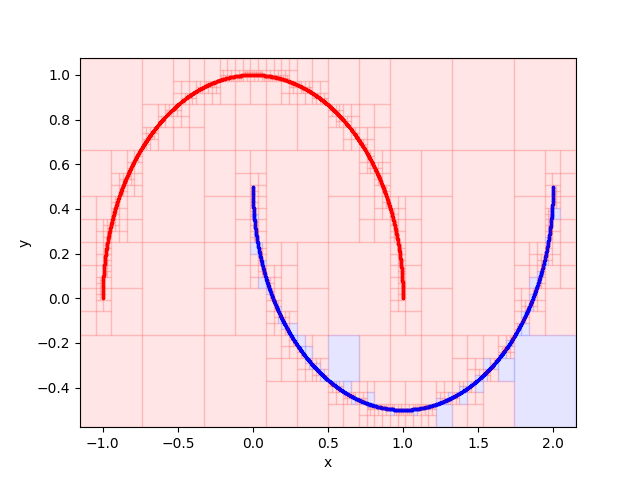
\includegraphics[width=.29\textwidth]{visual3000}}
%\end{center}
%\caption{Empirical accuracy/astuteness of different classifiers as a function of training sample size. Accuracy is shown in green, astuteness in purple. Left : Noiseless Setting. Right: Noisy Setting. Top Row: Histogram Classifier, Bottom Row: 1-Nearest Neighbor}
%\label{fig:1}
%\vskip -0.2in
%\end{figure}

\begin{figure}
\begin{subfigure}{0.31\textwidth}
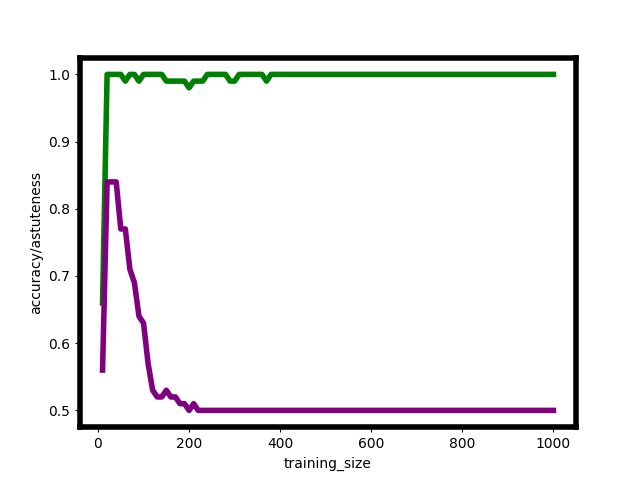
\includegraphics[width=\linewidth]{hist_noiseless_final}
%\caption{First subfigure} \label{fig:a}
\end{subfigure}\hspace*{\fill}
\begin{subfigure}{0.31\textwidth}
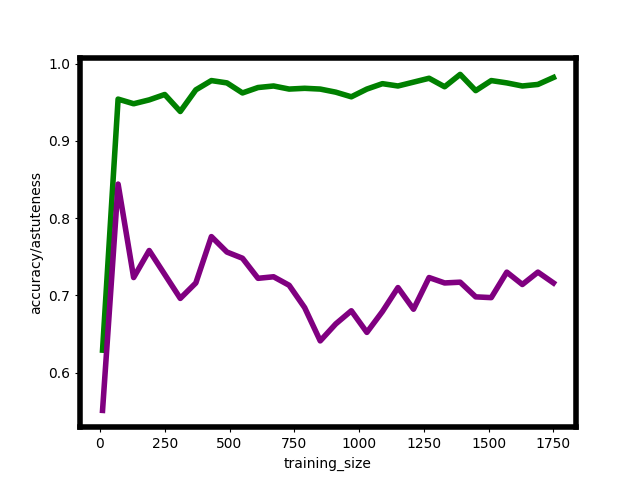
\includegraphics[width=\linewidth]{hist_noisy_final}
%\caption{Second subfigure} \label{fig:b}
\end{subfigure}\hspace*{\fill}
\begin{subfigure}{0.31\textwidth}
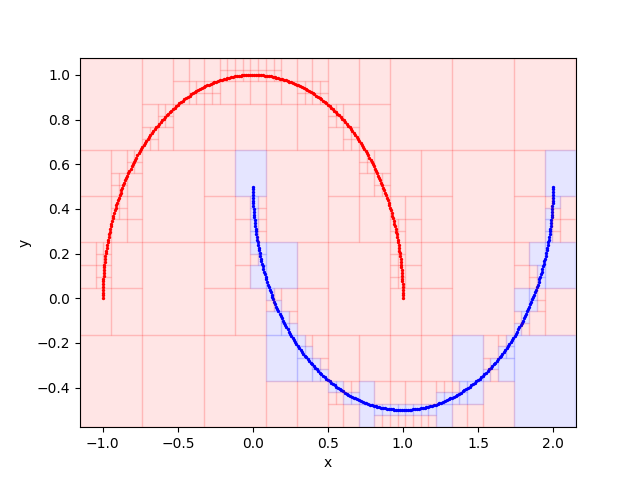
\includegraphics[width=\linewidth]{visual500}
%\caption{Fifth subfigure} \label{fig:e}
\end{subfigure}

\medskip
\begin{subfigure}{0.31\textwidth}
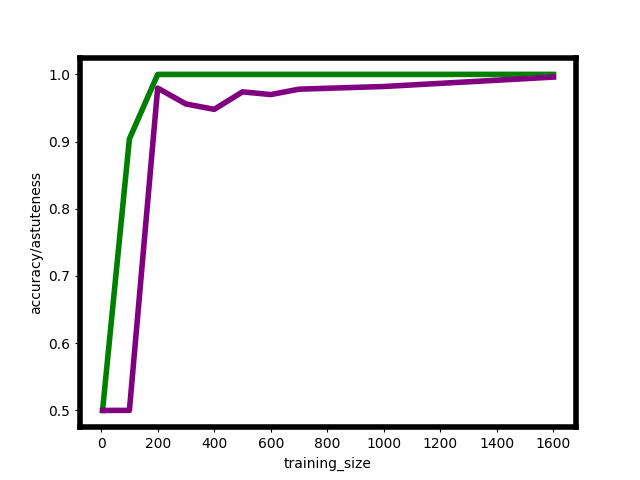
\includegraphics[width=\linewidth]{nn_noiseless_final}
%\caption{Third subfigure} \label{fig:c}
\end{subfigure}\hspace*{\fill}
\begin{subfigure}{0.31\textwidth}
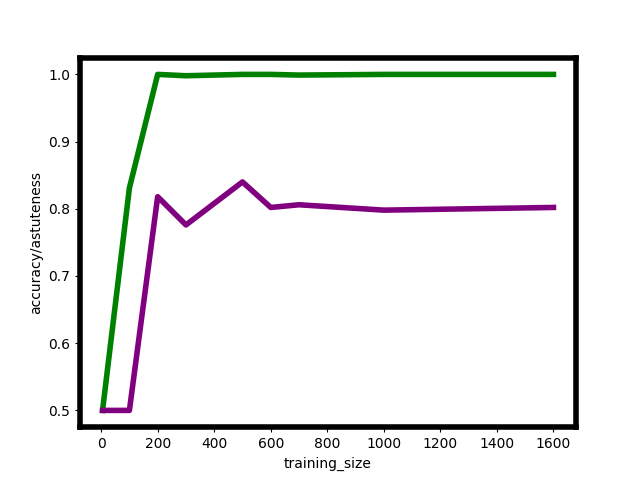
\includegraphics[width=\linewidth]{nn_noisy_final}
%\caption{Fourth subfigure} \label{fig:d}
\end{subfigure}\hspace*{\fill}
\begin{subfigure}{0.31\textwidth}
 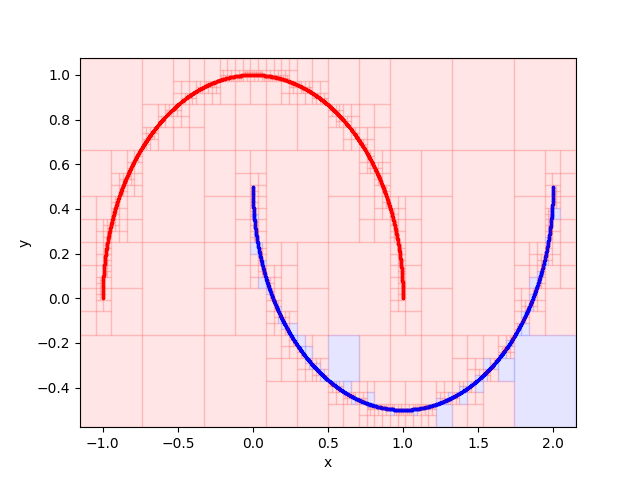
\includegraphics[width=\linewidth]{visual3000}
%\caption{Sixth subfigure} \label{fig:f}

\end{subfigure}

\caption{Empirical accuracy/astuteness of different classifiers as a function of training sample size. Accuracy is shown in green, astuteness in purple. Left : Noiseless Setting. Right: Noisy Setting. Top Row: Histogram Classifier, Bottom Row: 1-Nearest Neighbor} \label{fig:1}
\end{figure}

Our theoretical results are, by nature, large sample; we next validate how well they apply to the finite sample case by trying them out on a simple example. In particular, we ask the following question:

\begin{quote}
How does the robustness of non-parametric classifiers change with increasing sample size?
\end{quote}

This question is considered in the context of two simple non-parametric classifiers -- one nearest neighbor (which is guaranteed to be $r$-consistent) and histograms (which is not). To be able to measure performance with increasing data size, we look at a simple synthetic dataset -- the Half Moons. 

\subsection{Experimental Setup}

\paragraph{Classifiers and Dataset.} We consider two different classification algorithms -- one nearest neighbor (NN) and a Histogram Classifier (HC).  We use the Halfmoon dataset with two settings of the gaussian noise parameter $\sigma$, $\sigma = 0$ (Noiseless) and $\sigma =0.08$ (Noisy). For the Noiseless setting, observe that the data is already $0.1$-separated; for the Noisy setting, we use Adversarial Pruning (Algorithm~\ref{alg:gen}) with parameter $r = 0.1$ for both classification methods.

\paragraph{Performance Measure.} We evaluate robustness with respect to the $\ell_{\infty}$ metric, that is commonly used in the adversarial examples literature. Specifically, for each classifier, we calculate the {\em{empirical astuteness}}, which is the fraction of test examples on which it is astute.

Observe that computing the empirical astuteness of a classifier around an input $x$ amounts to finding the adversarial example that is {\em{closest to}} $x$ according to the $\ell_{\infty}$ norm. For the $1$-nearest neighbor, we do this using the optimal attack algorithm proposed by Yang et. al.~\cite{YRWC19}. For the histogram classifier, we use the optimal attack framework proposed by~\cite{YRWC19}, and show that the structure of the classifier can be exploited to solve the convex program efficiently. Details are in Appendix C.

We use an attack radius of $r = 0.1$ for the Noiseless setting, and $r = 0.09$ for the Noisy setting. For all classification algorithms, we plot the empirical astuteness as a function of the training set size. As a baseline, we also plot their standard accuracy on the test set. 

\subsection{Results}

The results are presented in Figure~\ref{fig:1}; the left two panels are for the Noiseless setting while the two center ones are for the Noisy setting.  

The results show that as predicted by our theory, for the Noiseless setting, the empirical astuteness of nearest neighbors converges to $1$ as the training set grows. For Histogram Classifiers, the astuteness converges to $0.5$ -- indicating that the classifier may grow less and less astute with higher sample size even for well-separated data. This is plausibly because the cell size induced by the histogram grows smaller with growing training data; thus, the classifier that outputs the default label $-1$ in empty cells is incorrect on adversarial examples that are close to a point with $+1$ label, but belongs to a different, empty cell. The rightmost panels in Figure~\ref{fig:1} provide a visual illustration of this process. 

For the Noisy setting, the empirical astuteness of adversarial pruning followed by nearest neighbors converges to $0.8$. For histograms with adversarial pruning, the astuteness converges to $0.7$, which is higher than the noiseless case but still clearly sub-optimal.

\subsection{Discussion}

Our results show that even though our theory is asymptotic, our predictions continue to be relevant in finite sample regimes. In particular, on well-separated data, nearest neighbors that we theoretically predict to be intrinsically robust is robust; histogram classifiers, which do not satisfy the conditions in Theorem~\ref{thm_stone_cons} are not. Our predictions continue to hold for data that is not well-separated. Nearest neighbors coupled with Adversarial
Pruning continues to be robust with growing sample size, while histograms continue to be non-robust. Thus our theory is confirmed by practice.

\section{Conclusion}

In conclusion, we rigorously analyze when non-parametric methods provide classifiers that are robust in the large sample limit. We provide a general condition that characterizes when non-parametric methods are robust on well-separated data, and show that Adversarial Pruning of~\cite{YRWC19} works on data that is not well-separated. 

Our results serve to provide a set of guidelines that can be used for designing non-parametric methods that are robust and accurate on well-separated data; additionally, we demonstrate that when data is not well-separated, preprocessing by adversarial pruning~\cite{YRWC19} does lead to optimally astute solutions in the large sample limit. 




%\input{chapters/chapter1/macros}
%\input{chapters/chapter1/introduction}
%\input{chapters/chapter1/related}
%\input{chapters/chapter1/definition}
%\input{chapters/chapter1/quantifying}
%\input{chapters/chapter1/visualizing}
%\input{chapters/chapter1/mitigation}
\graphicspath{{./chapters/chapter2/}}
%\newtheorem{thm}{Theorem}
%\newtheorem{lem}[thm]{Lemma}
%\DeclareMathOperator*{\argmax}{arg\,max}
%\DeclareMathOperator*{\argmin}{arg\,min}

\def\D{{\mathcal D}}
\def\Pphi{\overline{\Phi}}
\def\F{{\mathcal F}}
\def\N{{\mathcal N}}
%\def\R{{\mathbb R}}
\def\E{{\mathbb E}}
\def\A{\Pi}
\def\B{\Sigma}
\def\diam{\text{diam}}
\def\c{\mathcal L}
\def\l{\ell}
\def\seq{seq}
\def\R{\mathbb{R}}
\def\C{\mathcal C}
\def\p{p}
\def\s{size}
\def\L{\mathcal L}
\def\o{opt}
\def\H{\mathcal H}
\def\calH{\mathcal H}
\def\of{approxCluster}
\def\on{onlineCluster}
\def\R{\mathbb R}
\def\Y{\{\pm 1\}}
\def\U{\mathbb U}
\def\dd{\Delta}
\def\simp{{U\Delta}}
\def\g{g}
\def\rr{R}
\def\f{f}


\chapter{Sample Complexity of Robust Linear Classification on Separated Data} 

\section{Introduction}

Motivated by the use of machine learning in safety-critical settings, adversarially robust classification has been of much recent interest. Formally, the problem is as follows. A learner is given training data drawn from an underlying distribution $D$, a hypothesis class $\calH$, a robustness metric $d$, and a radius $r$. The learner's goal is to find a classifier $h \in \calH$ which has the lowest robust loss at radius $r$. The robust loss of a classifier is the expected fraction of examples where either $f(x) \neq y$ or where there exists an $x'$ at distance $d(x, x') \leq r$ such that $f(x) \neq f(x')$.  Robust classification thus aims to find a classifier that maximizes accuracy on examples that are distance $r$ or more from the decision boundary, where distances are measured according to the metric $d$.


In this work, we ask: how many samples are needed to learn a classifier with low robust loss when $\calH$ is the class of linear classifiers, and $d$ is an $\ell_p$-metric? Prior work has provided both upper~\cite{bartlett19, ravikumar20} as well as lower bounds~\cite{Schmidt18, ravikumar20} on the sample complexity of the problem. However, almost all look at settings where the data distribution itself is not separated --  data from different classes overlap or are close together in space. In this case, the classifier that minimizes robust loss is quite different from the one that minimizes error, which often leads to strong sample complexity gaps. Many real tasks where robust solutions are desired however tend to involve well-separated data~\cite{Yang20}, and hence it is instructive to look at what happens in these cases.

With this motivation, we consider in this work robust classification of data that is linearly $r$-separable. Specifically, there exists a linear classifier which has zero robust loss at robustness radius $r$. This case is thus the analog of the realizable case for robust classification, and we consider both upper and lower bounds in this setting.

For lower bounds, prior work \cite{Cullina18} shows that both standard and robust linear classification have VC-dimension $O(d)$, and consequently have similar bounds on the expected loss in the worst case. However, these results do not apply to this setting since we are specifically considering well-separated data, which greatly restricts the set of possible worst-case distributions.  For our lower bound, we provide a family of distributions that are linearly $r$-separable and where the maximum margin classifier, given $n$ independent samples, has error $O(1/n)$. In contrast, any algorithm for finding the minimum robust loss classifier has robust loss at least $\Omega(d/n)$, where $d$ is the data dimension. These bounds hold for all $\ell_p$-norms provided $p > 1$, including $p=2$ and $p=\infty$. Unlike prior work, our bounds do not rely on the difference in loss between the solutions with optimal robust loss and error, and hence cannot be obtained by prior techniques. Instead, we introduce a new geometric construction that exploits the fact that learning a classifier with low robust loss when data is linearly $r$-separated requires seeing a certain number of samples close to the margin.

For upper bounds, prior work \cite{bartlett19} provides a bound on the Rademacher complexity of adversarially robust learning, and show that it can be worse than the standard Rademacher complexity by a factor of $d^{1/q}$ for $\ell_p$-norm robustness where $1/p + 1/q = 1$. Thus, an interesting question is whether dimension-independent bounds, such as those for the accuracy under large margin classification, can be obtained for robust classification as well. Perhaps surprisingly, we show that when data is really well-separated, the answer is yes. Specifically, if the data distribution is linearly $r + \gamma$-separable, then there exists an algorithm that will find a classifier with robust loss $O(\Delta^2/\gamma^2 n)$ at radius $r$ where $\Delta$ is the diameter of the instance space. Observe that much like the usual sample complexity results on SVM and perceptron, this upper bound is independent of the data dimension and depends only on the excess margin (over $r$). This establishes that when data is really well-separated, finding robust linear classifiers does not require a very large number of samples. 

While the main focus of this work is on linear classifiers, we also show how to generalize our upper bounds to Kernel Classification, where we find a similar dynamic with the loss being governed by the excess margin in the embedded kernel space. However, we defer a thorough investigation of robust kernel classification as an avenue for future work.

Our results imply that while adversarially robust classification may be more challenging than simply accurate classification when the classes overlap, the story is different when data is well-separated. Specifically, when data is linearly (exactly) $r$-separable, finding an $r$-separated solution to robust loss $\epsilon$ may require $\Omega(d/\epsilon)$ samples for some distribution families where finding an accurate solution is easier. Thus in this case, there is a gap between the sample complexities of robust and simply accurate solutions, and this is true regardless of the $\ell_p$ norm in which robustness is measured. In contrast, if data is even more separated -- linearly $r + \gamma$-separable --  then we can obtain a dimension-independent upper bound on the sample complexity, much like the sample complexity of SVMs and perceptron. Thus, how separable the data is matters for adversarially robust classification, and future works in the area should consider separability while discussing the sample complexity.

\subsection{Related Work}

There is a large body of work \cite{Carlini17, Liu17, Papernot17, Papernot16, Szegedy14, Hein17, Katz17, Wu16,Steinhardt18, Sinha18} empirically studying adversarial examples primarily in the context of neural networks. Several works \cite{Schmidt18, Raghunathan20, Tsipras19} have empirically investigated trade-offs between robust and standard classification.

On the theoretical side, this phenomenon has been studied in both the parametric and non-parametric settings. On the parametric side, several works \cite{loh18, attias19, Srebro19, bartlett19, pathak20} have focused on finding distribution agnostic bounds of the sample complexity for robust classification. In \cite{Srebro19}, Srebro et. al. showed through an example that the VC dimension of robust learning may be much larger than standard or accurate learning indicating that the sample complexity bounds may be higher. However, their example did not apply to linear classifiers. 

\cite{Kane20} considers learning linear classifiers robustly, but is primarily focused on computational complexity as opposed to sample complexity.

In \cite{bartlett19}, Bartlett et. al. investigated the Rademacher complexity of robustly learning linear classifiers as well as neural networks. They showed that in both cases, the robust Rademacher complexity can be bounded in terms of the dimension of the input space -- thus indicating a possible gap between standard and robust learning. However, as with the works considering VC dimension, this work is fundamentally focused on upper bounds  -- they do not show true lower bounds on data requirements.

Because of it's simplicity and elegance, the case where the data distribution is a mixture of Gaussians has been particularly well-studied. The first such work was \cite{Schmidt18}, in which Schmidt et. al. showed an $\Omega(\sqrt{d})$ gap between the standard and robust sample complexity for a mixture of two Gaussians using the $\ell_\infty$ norm. This was subsequently expanded upon in \cite{Bhagoji19}, \cite{robey20} and  \cite{ravikumar20}. \cite{Bhagoji19} introduces a notion of ``optimal transport," which they subsequently apply to the Gaussian case, deriving a closed form expression for the optimally robust linear classifier. Their results apply to any $\ell_p$ norm. \cite{robey20} applies expands upon \cite{Schmidt18} by consider mixtures of three Gaussians in both the $\ell_2$ and $\ell_\infty$ norms. Finally, \cite{ravikumar20} fully generalizes the results of \cite{Schmidt18} providing tight upper and lower bounds on the standard and robust sample complexities of a mixture of two Gaussians, in any norm (including $\ell_p$ for $p \in [1, \infty]$). \cite{Schmidt18} and \cite{ravikumar20} bear the most relevance with our work, and we consequently carefully compare our results in section \ref{sec:comparison}.

Another approach for lower and upper bounds on sample complexities for linear classifiers can be found in \cite{Cullina18}, which examines the robust VC dimension of learning linear classifiers. They show that the VC dimension is $d+1$, just as it is in the standard case. This implies that the bounds in the robust case match the bounds in the standard case and in particular shows a lower bound of $\Omega(d/n)$ on the expected loss of learning a robust linear classifier from $n$ samples.

While this result appears to match our lower bound, there is a crucial distinction between the bounds. Our bound implies that there exists some distribution with a large $\ell_2$ margin for which the expected robust loss must be $\Omega(d/n)$. On the other hand, standard results about learning linear classifiers on large margin data implies that the expected standard loss will be $O(1/n)$ (when running the max-margin algorithm). For this reason, our paper provides a case in the well-separated setting in which learning linear classifiers is provably more difficult (in terms of sample complexity) in the robust setting than in the standard setting. By contrast, \cite{Cullina18} does not show this. Their paper only implies (through standard VC constructions) the existence of \textit{some} distribution that is difficult to learn, and the standard PAC bounds cannot ensure that such a distribution also has a large $\ell_2$ margin.

In the non-parametric setting, there are several works which contrast standard learning with robust learning. \cite{WJC18} considers the nearest neighbors algorithm, and shows how to adapt it for converging towards a robust classifier. In \cite{YRWC19}, Yang et. al. propose the $r$\textit{-optimal classifier}, which is the robust analog of the Bayes optimal classifier. Through several examples they show that it is often a fundamentally different classifier - which can lead to different convergence behavior in the standard and robust settings. \cite{Bhattacharjee20} unified these approaches by specifying conditions under which non-parametric algorithms can be adapted to converge towards the $r$-optimal classifier, thus introducing $r$-consistency, the robust analog of consistency.

\section{Preliminaries}
We consider binary classification over $\R^d \times \Y$. Our metric of choice is the $\ell_p$ norm, where $p > 1$ (including $p = \infty$) is arbitrary. For $x \in \R^d$, we will use $||x||_p$ to denote the $\ell_p$ norm of $x$, and consequently will use $||x - y ||_p$ to denote the $\ell_p$ distance between $x$ and $y$. We will also let $\ell_q$ denote the dual norm to $\ell_p$ - that is, $\frac{1}{q} + \frac{1}{p}= 1$.

 We use $B_p(x,r)$ to denote the closed $\ell_p$ ball with center $x$ and radius $r$. For any $S \subset \R^d$, we let $diam_p(S)$ denote its diameter: that is, $diam_p(S) = \sup_{x, y \in S} ||x - y||_p.$

\subsection{Standard and Robust Loss}

In classical statistical learning, the goal is to learn an accurate classifier, which is defined as follows:

\begin{defn}
Let $\D$ be a distribution over $\R^d \times \Y$, and let $f \in \Y^{\R^d}$ be a classifier. Then the \textbf{standard loss} of $f$ over $\D$, denoted $\L(f, \D)$, is the fraction of examples $(x,y) \sim \D$ for which $f$ is not accurate. Thus $$\L(f, \D) = P_{(x,y) \sim \D}[f(x) \neq y].$$
\end{defn}

Next, we define robustness, and the corresponding robust loss.

\begin{defn}
A classifier $f \in \Y^{\R^d}$ is said to be \textbf{robust} at $x$ with radius $r$ if $f(x) = f(x')$ for all $x' \in B_p(x,r)$. 
\end{defn}


\begin{defn}
The \textbf{robust loss} of $f$ over $\D$, denoted $\L_r(f, \D)$, is the fraction of examples $(x,y) \sim \D$ for which $f$ is either inaccurate at $(x,y)$, or $f$ is not robust at $(x,y)$ with radius $r$. Observe that this occurs if and only if there is some $x' \in B_p(x,r)$ such that $f(x') \neq y$. Thus $$\L_r(f, \D) = P_{(x, y) \sim \D}[\exists x' \in B_p(x,r)\text{ s.t. }f(x') \neq y].$$ 
\end{defn}

\subsection{Expected Loss and  Sample Complexity}

The most common way to characterize the performance of a learning algorithm is through an $(\epsilon, \delta)$ guarantee, which computes $\epsilon_n, \delta_n$ such that an algorithm trained over $n$ samples has loss at most $\epsilon_n$ with probability at least $1 - \delta_n$. 

In this work, we use the simpler notion of \textit{expected loss}, which is defined as follows: 

\begin{defn}
Let $A$ be a learning algorithm and let $\D$ be a distribution over $\R^d \times \{\pm 1\}$. For any $S \sim \D^n$, we let $A_S$ denote the classifier learned by $A$ from training data $S$. Then the \textbf{expected standard loss} of $A$ with respect to $\D$, denoted $EL^n(A, \D)$ where $n$ is the number of training samples, is defined as $$E\L^n(A, \D) = \E_{S \sim \D^n} \L(A_S, \D).$$ Similarly, we define the \textbf{expected robust loss} of $A$ with respect to $\D$ as $$E\L_r^n(A , \D) = \E_{S \sim \D^n}\L_r(A_S, \D).$$ 
\end{defn}

Our main motivation for using this criteria is simplicity. Our primary goal is to compare and contrast the performances of algorithms in the standard and robust cases, and this contrast clearest when the performances are summarized as a single number (namely the expected loss) rather than an $(\epsilon, \delta)$ pair. 

Next, we address the notion of sample complexity. As above, sample complexity is typically defined as the minimum number of samples needed to guarantee $(\epsilon, \delta)$ performance. In this work, we will instead define it solely with respect to $\epsilon$, the expected loss. 

\begin{defn}
Let $\D$ be a distribution over $\R^d \times \{\pm 1\}$ and $A$ be a learning algorithm. Then the \textbf{standard sample complexity} of $A$ with respect to $\D$, denoted $m^\epsilon(A, \D)$, is the minimum number of training samples needed such that $A$ has  expected standard loss at most $\epsilon$. Formally, $$m^\epsilon(A, \D) = \min(\{n: E\L^n(A, D) \leq \epsilon\}).$$ Similarly, we can define the \textbf{robust sample complexity} as $$m_r^\epsilon(A, \D) = \min(\{n: E\L^n(A, D) \leq \epsilon\}).$$
\end{defn}



%\input{chapters/chapter1/macros}
%\input{chapters/chapter1/introduction}
%\input{chapters/chapter1/related}
%\input{chapters/chapter1/definition}
%\input{chapters/chapter1/quantifying}
%\input{chapters/chapter1/visualizing}
%\input{chapters/chapter1/mitigation}
\graphicspath{{./chapters/chapter3/}}
%\newtheorem{thm}{Theorem}
%\newtheorem{lem}[thm]{Lemma}
%\DeclareMathOperator*{\argmax}{arg\,max}
%\DeclareMathOperator*{\argmin}{arg\,min}

\newtheorem*{rep@theorem}{\rep@title}
\newcommand{\newreptheorem}[2]{%
\newenvironment{rep#1}[1]{%
 \def\rep@title{#2 \ref{##1}}%
 \begin{rep@theorem}}%
 {\end{rep@theorem}}}
\makeatother
%\newtheorem{thm}{Theorem}
\newreptheorem{thm}{Theorem}
%\newtheorem{lem}[thm]{Lemma}
\newreptheorem{lem}{Lemma}
\newtheorem{prop}[thm]{Proposition}
\newreptheorem{prop}{Proposition}
%\newtheorem{cor}[thm]{Corollary}
\newreptheorem{cor}{Corollary}
\newtheorem{claim}{Claim}

\newtheorem{innercustomgeneric}{\customgenericname}
\providecommand{\customgenericname}{}
\newcommand{\newcustomtheorem}[2]{%
  \newenvironment{#1}[1]
  {%
   \renewcommand\customgenericname{#2}%
   \renewcommand\theinnercustomgeneric{##1}%
   \innercustomgeneric
  }
  {\endinnercustomgeneric}
}

\newcustomtheorem{customthm}{Theorem}
\newcustomtheorem{customlemma}{Lemma}
\newcustomtheorem{customprop}{Proposition}

\newcommand{\defref}[1]{Definition~\ref{#1}}
\newcommand{\tabref}[1]{Table~\ref{#1}}
\newcommand{\figref}[1]{Fig.~\ref{#1}}
\newcommand{\eqnref}[1]{\text{Eq.}~(\ref{#1})}
\newcommand{\secref}[1]{\textnormal{Section}~\ref{#1}}
\newcommand{\appref}[1]{Appendix \ref{#1}}
\newcommand{\stepref}[1]{Step \ref{#1}}
%\newcommand{\appref}[1]{the Appendix} % for short version of the paper
\newcommand{\thmref}[1]{Theorem~\ref{#1}}
\newcommand{\corref}[1]{Corollary~\ref{#1}}
\newcommand{\propref}[1]{Proposition~\ref{#1}}
\newcommand{\lemref}[1]{Lemma~\ref{#1}}
\newcommand{\conref}[1]{Condition~\ref{#1}}
\newcommand{\assref}[1]{Assumption~\ref{#1}}
\newcommand{\algref}[1]{Algorithm~\ref{#1}}
\newcommand{\egref}[1]{Example~\ref{#1}}
\newcommand{\algoref}[1]{Algorithm~\ref{#1}}

\newcommand{\op}[1]{\operatorname{#1}}
\newcommand{\paren} [1] {\ensuremath{ \left( {#1} \right) }}
\newcommand{\parenb} [1] {\ensuremath{ \big( {#1} \big) }}
\newcommand{\bigparen} [1] {\ensuremath{ \Big( {#1} \Big) }}
\newcommand{\biggparen} [1] {\ensuremath{ \bigg( {#1} \bigg) }}
\newcommand{\Biggparen} [1] {\ensuremath{ \Bigg( {#1} \Bigg) }}
\newcommand{\bracket}[1]{\left[#1\right]}
\newcommand{\tuple}[1]{\ensuremath{\left\langle #1 \right\rangle}}
\newcommand{\set}[1]{\ensuremath{\left\{#1\right\}}}
\newcommand{\curlybracket}[1]{\ensuremath{\left\{#1\right\}}}
\newcommand{\norm}[2]{\ensuremath{\left\langle#1,\:#2\right\rangle_{\cH_{\rK}}}}
\newcommand{\normg}[2]{\ensuremath{\left\langle#1,\:#2\right\rangle}}
\newcommand{\condcurlybracket}[2]{\ensuremath{\left\{#1\left\lvert\:#2\right.\right\}}}
\newcommand{\inmod}[1]{\ensuremath{\left\lvert\left\lvert#1\right\rvert\right\rvert}}
\newcommand{\boldalpha}{\ensuremath{\boldsymbol{\alpha}}}

\def\ind{\mathbbm{1}}
\def\oc{Online\_Cluster}
\def\ocns{No\_Sub\_Cluster}
\def\mem{\mathcal M}
\def\E{\mathbb{E}}
\def\R{\mathbb{R}}
\def\OC{\text{OC}}
\def\cH{\mathcal H}
\def\reals{\mathbb{R}}
\def\cD{\mathcal D}
\def\Ev{\mathbb{E}}
\def\cO{\mathcal O}
\def\cX{\mathcal X}
\def\cU{\mathcal U}
\def\cM{\mathcal M}



\chapter{Robust Empirical Risk Minimization with Tolerance} 

\section{Introduction}

Adversarially robust classification is a staple of modern machine learning. In the robust setting, along with meeting standard accuracy guarantees, predictions made by a learner at test time must additionally be robust to adversarial perturbations to the input, typically defined by a fixed family $\mathcal{U}=\{U_x\}_{x \in X}$ of possible perturbations. Developing robust algorithms with provable guarantees has been an important research direction in recent years, both for parametric \cite{loh18, attias19, Srebro19, bartlett19, pathak20} and non-parametric \cite{WJC18, YRWC19, Bhattacharjee20, Bhattacharjee21} classifiers, but understanding the performance of even the most basic algorithms in the setting remains open.

In this work, we study one of the simplest, most fundamental algorithmic paradigms in learning, a classical method called \textit{empirical risk minimization} (ERM). In the robust setting, an algorithm is said to be an empirical risk minimizer (RERM) if it always outputs a hypothesis in the class with minimal \textit{robust} risk over its training data. In the standard setting, it is a classical result that any learnable class is learnable (near-optimally) by any ERM. Unfortunately, this is known to fail drastically in the robust setting---\citet{Srebro19} showed that there exist finite VC classes, $\mathcal{H}$, where no algorithm outputting hypotheses in $\mathcal{H}$ (called a \textit{proper} learner) can converge towards the optimal classifier, even with arbitrary amounts of training data. Conversely, such classes \textit{are} in fact robustly learnable, but require complicated improper learning rules and a potentially exponential number of samples.

The failure of Robust ERM for general classes raises an interesting question: \textit{are there natural sufficient conditions for the success of RERM?} One obvious answer to this question is the notion of robust VC dimension, a combinatorial parameter promising the success of RERM. However, bounding robust VC is typically difficult, and such results are only known for very specialized examples of classifiers and robustness regions (e.g.\ linear classifiers under fixed-radius balls \citep{Cullina18} or other simple margin structures \cite{pathak20}, or VC-classes under finite perturbation sets \citep{attias19}). To our knowledge there are no corresponding results for more general robustness regions and hypothesis classes beyond these special cases.

% Although there is some recent work indicating this may be possible (for example  gives sample complexity bounds for learning robust linear classifiers), these works are typically restricted to specific examples of classifiers and robustness regions, with the most common example being the case that all robustness regions are ball within some norm of a fixed radius. 
% However, to our knowledge, there are no corresponding results for the general case of arbitrary robustness region.

Given the current failure of combinatorial techniques in this setting, one might instead hope to show RERM works given sufficiently nice \textit{geometric} conditions on the hypothesis class. Sadly, this is not the case. We show that there exist robustness regions for which RERM (indeed any proper algorithm) fails even for settings as simple as (bounded) linear classifiers.
\begin{thm}[Failure of RERM for Linear Classifiers]\label{thm:intro1}
For any $W>0$ and $d>1$, let $\cH_W$ denote the set of linear classifiers with distance at most $W$ from the origin. Then there exists a set of robustness regions $U$ over $\R^d$ such that for any proper learning algorithm $L$ there exists a distribution $\cD$ for which the following hold:
\begin{itemize}
	\item \textbf{$\cD$ is realizable}: There exists $h^* \in \cH_W$ such that $\ell_U(h^*, \cD) = 0$.
	\item \textbf{$L$ has high error}: With probability at least $\frac{1}{7}$ over $S \sim \cD^m$, $\ell_U(L(S), \cD) > \frac{1}{8}$. 
\end{itemize}
\end{thm}

With this in mind, we turn our attention to a different approach: relaxing the notion of robustness itself. We'll consider a recent model of \citet{Urner22} called \textit{tolerant} robust learning. In the tolerant setting, the learner is only required to compete with the best loss over a relaxed family of perturbation sets $\mathcal{U}^\gamma$ for a (potentially arbitrary) tolerance parameter $\gamma >0$. \citet{Urner22} studied this setting in the special case of radius $r$ balls, where the learner competes with robust error against $r(1 + \gamma)$-balls. Under this framework, \citet{Urner22} give an algorithm with PAC-guarantees for VC classes using significantly fewer samples, but their techniques remain improper and only hold for the simplest robustness setting.

In this work, we show that a simple variant of RERM in the tolerant model indeed succeeds under natural geometric conditions on the hypothesis class. In particular, we study a notion of smoothness called \textit{regularity}, which roughly promises that every point in the instance space should be contained in some ball of the same label. This captures many well-studied settings, such as cases where the decision boundaries are compact, differential manifolds in $\mathbb{R}^d$.
\begin{thm}[Tolerant RERM for Regular Classes]\label{thm:upper_bound1}
Let $\cH$ be a regular hypothesis class with VC dimension $v$ over $\mathbb{R}^d$, and let $\mathcal{U}$ be any set of robustness regions. Then $TolRERM$ tolerantly PAC-learns $(\cH, \mathcal{U})$ with tolerant sample complexity 
\[
m(\epsilon, \delta, \gamma)  = O\left( \frac{vd\log \frac{d\text{Diam}(U)}{\epsilon\gamma\delta}}{\epsilon^2}\right),
\]
where $\text{Diam}(U)$ denotes the maximum $\ell_2$ diameter across robustness regions $U_x$. 
\end{thm}
Theorem \ref{thm:upper_bound1} matches the sample complexity given in \citet{Urner22} up to logarithmic factors and enjoys the additional benefits of applying to more general robustness regions along with its properness and general algorithmic simplicity. For completeness, we also analyze our algorithm's performance over non-regular classifiers in Appendix \ref{sec:proof_extension}, and show that it has a similar performance albeit at the cost of replacing the VC-dimension with $v_{\text{ball}}$, the robust VC dimension of $\cH$ over balls of a fixed radius. Thus, for non-regular hypothesis classes, our algorithm gives a reduction from arbitrary robustness regions to the case where they are all balls of a fixed radius.

Finally it's worth noting that while \citet{Urner22} only requires sampling access to the perturbation sets, stronger access such as an empirical risk minimizer is inevitable in the general setting where $\mathcal{U}$ is unknown. We show that there exists hypothesis classes where $\Omega((\frac{D}{\gamma})^d)$ queries to a sampling oracle are required for robust learning with tolerance if no other interaction with $U_x$ is permitted.

While Theorem \ref{thm:upper_bound1} gives a natural sufficient condition for the success of RERM in relaxed settings, many questions in this direction remain wide open. It would be interesting to identify a necessary condition for the success of RERM, both in the tolerant and original robust models. Furthermore, it should be noted that while we prove RERM fails to learn nice classes in the latter, the perturbation family we use to achieve this is highly combinatorial. As such, there is still hope that RERM may be sufficient in the traditional setting under \textit{joint} niceness conditions on $\mathcal{H}$ and $\mathcal{U}$, though the close interplay between the two families seems to make identifying such a condition difficult, if it is indeed possible at all.


\section{Related Work}

Much of the work on adversarial robustness \citep{Carlini17, Liu17, Papernot17, Papernot16, Szegedy14, Hein17, Katz17, Wu16,Steinhardt18, Sinha18} is done in the context of neural networks.

On the theoretical side, there has been a recent focus on developing algorithms with guarantees in convergence towards an optimal classifier. On the parametric side, several works \citep{loh18, attias19, Srebro19, bartlett19, pathak20, Cullina18} have focused on distribution agnostic bounds on the amount of data required to converge towards the optimal classifier in a given hypothesis class. For example, \citet{Srebro19} showed through an example that the VC dimension of robust learning may be much larger than standard or accurate learning indicating that the sample complexity bounds may be higher. There has also been some work considering the computation complexity required for robust learning such as \citet{Kane20}.


Aside from \citet{Urner22}, there are several works which also consider variations on robust learning with tolerance. \citet{YRWC19} and \citet{Bhattacharjee20} show that certain non-parametric algorithms exhibit a type of tolerant behavior when robustness regions are constrained to be balls of radius $r$. \citet{Omar22} considers robustness in the \textit{transductive learning setting}. Their work employs a similar idea to \citet{Urner22} in that they consider expanded perturbation sets when giving their formal guarantees. However, their expansions are not based on tolerance $\gamma > 0$.

\section{Preliminaries}
Let $\cH$ be a family of binary classifiers $\{h: \mathbb{R}^d \to \{\pm 1\}\}$, and $U = \{U_x \subseteq \R^d: x \in \reals^d\}$ any set of robustness regions. 
% We make no assumptions about $U$ except for each $U_x$ having $\ell_2$ diameter at most $D$. 
We define the robust loss function with respect to $U$ as follows.
\begin{defn}
Let $h \in \cH$ be a classifier and $(x,y) \in \reals^d \times \{\pm 1\}$ be a labeled point. Then the \textbf{robust loss} of $h$ over $(x, y)$, denoted $\ell_U(h, (x,y))$, is defined as 
\begin{align*}
  \ell_{U}(h, (x,y)) = \begin{cases} 1 & \exists x' \in U_x\text{ such that }h(x') \neq y \\0 & \text{otherwise.} \end{cases}.  
\end{align*}
%$$$$ 
That is, $h$ achieves a loss of $0$ only if it labels all points in $U_x$ as $y$. 
\end{defn}

For a distribution, $\cD$ over $\reals^d \times \{\pm 1\}$, we let $ \ell_U(h, \cD)$ denote the expected loss $h$ pays over a labeled point drawn from $\cD$. That is, $\ell_U(h, \cD) = \Ev_{(x,y) \sim \cD}[\ell_U(h, (x,y))]$. 

Similarly, for a set of $n$ labeled points, $S$, we let $\ell_U(h, S)$ denote the average robust loss $h$ pays over $S$. that is, $\ell_U(h, S) = \frac{1}{n} \sum_{i=1}^n \ell_U(h, (x_i, y_i))$. 

We will also use $||x - x'||$ to denote the $\ell_2$ distance between $x$ and $x'$, and $B(x, r)$ to denote the (closed) $\ell_2$ ball centered at $x$ with radius $r$.

\subsection{Robust PAC-learning}

We now review a natural generalization of PAC learning to the robust setting called robust PAC-learning \citep{Srebro19}. 

\begin{defn}\label{defn:rob_pac}
Let $\cH$ be a hypothesis class and $U$ be a set of robustness regions. A learner $L$ \textbf{robustly PAC-learns} $(\cH, U)$ if for every  $\epsilon, \delta > 0$, there exists $m(\epsilon, \delta)$ such that for all $n \geq m(\epsilon, \delta)$, for all data distributions, $\cD$, with probability $1-\delta$ over $S \sim \cD^n$, $$\ell_{U}(\hat{h}, \cD) \leq \min_{h \in \cH} \ell_{U}(h, \cD) + \epsilon,$$ where $\hat{h} = L(S)$ denotes the classifier in $\cH$ outputted by $L$ from training sample $S$. $m(\epsilon, \delta)$ is said to be the \textbf{sample complexity} of $L$ with respect to $(\cH, U)$. 
\end{defn}

Algorithms that are able to robustly PAC-learn a pair $(\cH, U)$ are the natural robust analogs of standard learning algorithms, and thus an important question is understanding how the sample complexities, $m(\epsilon, \delta)$, for doing so are bounded.

\section{Robust Empirical Risk Minimization on Linear Classifiers}

\looseness-1\citet{Srebro19} showed that there exist hypothesis classes $\cH$ with bounded VC dimension, and robustness regions $U$, such that proper robust PAC-learning is not possible, meaning no matter how much data one is allowed, there always exists a distribution where the learner will suffer high robust loss.

However, for many practical examples, this does not appear to be the case -- for example, \cite{Cullina18} showed that when $\cH$ is the set of all linear classifiers and $U$ is the set of robustness regions with $U_x = B(x, r)$, the sample complexity of robustly learning with RERM is at most $m(\epsilon, \delta) = \tilde{O}\left(\frac{d}{\epsilon^2}\right)$, matching the standard complexity for linear classification. 

Motivated by recent interest in more general robustness regions than balls of a fixed radius, we consider the case where $\cH$ is a natural hypothesis class, but $U$ is a potentially arbitrary robustness region. That is, we ask the following question: are there examples of natural hypothesis classes for which there exist robustness regions leading to arbitrary high sample complexities?

Unfortunately, the answer turns out to be yes. To show this, we begin by defining the natural hypothesis class of \textit{bounded} linear classifiers.
\begin{defn}\label{defn:bounded_linear}
A $W$-bounded linear classifier, $f: \R^d \to \R^d$, is a linear classifier $h$ whose decision boundary has distance at most $W$ from the origin. That is, there exist $w \in \R^d$ and , $b\in \R$ with $\frac{|b|}{||w||} \leq W$ such that $$h(x) = \begin{cases}1 & \langle w, x \rangle + b \geq 0 \\ -1 & otherwise \end{cases}.$$ We let $\cH_W$ denote the class of all $W$-bounded linear classifiers
\end{defn}
The boundedness condition, $W$, can be thought of as a regularization term which is common during any kind of practical optimization.

We now show that there exist robustness regions, $U$, for which $(\cH_W, U)$ is not robustly PAC-learnable, even in the realizable setting. For convenience, we restate Theorem \ref{thm:lower_bound1} from the introduction.

% \begin{theorem}\label{thm:lower_bound}
% Let $W > 0$ be arbitrary and let $m > 0$ be any integer. Then there exists a set of robustness regions $U$ over $\R^d$ such that for any learning algorithm $L$, there exists a distribution $\cD$ for which the following hold:
% \begin{itemize}
% 	\item There exists $h^* \in \cH_W$ such that $\ell_U(h^*, \cD) = 0$.
% 	\item With probability at least $\frac{1}{7}$ over $S \sim \cD^m$, $\ell_U(L(S), \cD) > \frac{1}{8}$. 
% \end{itemize}
% \end{theorem}
\begin{thm}\label{thm:lower_bound1}
For any $W>0$ and $d>1$, there exists a set of robustness regions $U$ over $\R^d$ such that for any learning algorithm $L$ there exists a distribution $\cD$ for which the following hold:
\begin{itemize}
	\item \textbf{$\cD$ is realizable}: There exists $h^* \in \cH_W$ such that $\ell_U(h^*, \cD) = 0$.
	\item \textbf{$L$ has high error}: With probability at least $\frac{1}{7}$ over $S \sim \cD^m$, $\ell_U(L(S), \cD) > \frac{1}{8}$. 
\end{itemize}
\end{thm}

% Theorem \ref{thm:lower_bound} immediately implies that there exist $U$ for which the sample complexity, $m(\epsilon, \delta)$ is arbitrarily high for any learner.
Theorem \ref{thm:lower_bound1} consequently shows that the observations made in \cite{Srebro19} hold even over practical hypothesis classes such as (bounded) linear classifiers.

To prove Theorem \ref{thm:lower_bound1}, we begin with the following critical lemma.
\begin{lem}\label{lem:finding_shatter}
For every $M \in \mathbb{N}$ there exists a family of $M$ subsets of $\R^d$
\[
Z^{(M)} \coloneqq \left\{Z^{(M)}_1, Z^{(M)}_2, \dots, Z^{(M)}_M\right\}
\]
satisfying the following conditions:
\begin{itemize}
	\item For every $h \in \cH_W$, there exists $z \in Z^{(M)}$ such that $h(z) = 1$.
	\item For every $1 \leq i \leq M$, there exists $h_i \in \cH_W$ such that $h_i(z) = -1$ for all $z \in \cup_{j \neq i} Z^{(M)}_j$.
	\item The sets $\{Z^{(M)}\}_{M \in \mathbb{N}}$ are mutually disjoint.
\end{itemize}
\end{lem}

\begin{proof}
Let $\{\beta_i\}_{i \in \mathbb{N}} > 0$ be a strictly decreasing sequence of sufficiently small real numbers (that we will specify later). For notational simplicity, fix an $M \in \mathbb{N}$ and write $\beta=\beta_M$ and $W' = (1 + \beta)W$. For any $r > 0$, let $S_r^{d-1}$ denote the $(d-1)$-sphere centered at the origin of radius $r$.

Observe that for any $x \in S_W^{d-1}$, there exists a unique classifier $h \in \cH_W$ whose decision boundary is tangent to $S_W^{d-1}$ at $x$ so that $h(x) = 1$. We denote this classifier as $h_x$. It follows that the set of all points on $S_{W'}^{d-1}$ that $h_x$ classifies as $1$ can be easily characterized in terms of $x$. In particular, by the definition of $h_x$, it follows from geometry that
\begin{equation}\label{eqn:lol_i_literally_used_law_of_cosines}
\curlybracket{z: h_x(z) = 1, z \in S_{W'}^{d-1}} = \curlybracket{z: ||z - (1+\beta)x|| \leq W\sqrt{2\beta(\beta + 1)}, z \in S_{W'}^{d-1}}.
\end{equation}

Let $r_\beta = 2W\sqrt{2\beta(\beta + 1)}$, and let $z_1, z_2, \dots, z_{M_{\beta}}$ denote a a greedy $r_\beta$ cover of $S_{W'}^{d-1}$, meaning that points are successively selected from $S_{W'}^{d-1}$ until no point with distance strictly greater than $r_\beta$ from all other points can be selected. Finally, define $Z_i=Z_i^{(M)}$ as the set of elements in $S_{W'}^{d-1}$ with nearest neighbor $z_i$ (ties broken arbitrarily).

We claim that this construction suffices for $M_\beta \geq M$. First, observe that $\lim_{\beta \to 0} r_\beta = 0$, which means that for sufficiently small $\beta$ that $M_\beta$ will be arbitrarily large (thus satisfying $M_\beta \geq M$). So select any $\beta$ for which this hold, and merge enough regions so that we are left with exactly $M$ regions (i.e. set $Z_{M} = \cup_{i = M}^{M_\beta} Z_i$). Note that we can always choose $0<\beta< \beta_{M-1}$ since the naturals can be embedded into any interval. We now verify the two stipulations of Lemma \ref{lem:finding_shatter}. 

The first stipulation clearly holds since $\{Z_i\}_{i=1}^M$ partition $S_{W'}^{d-1}$ and every halfspace $h \in \cH_W$ intersects the latter by construction.

For the second stipulation, observe that for any $i$, the ball centered at $z_i$ of radius $\frac{r_\beta}{2}$, $B\left(z_i, \frac{r_\beta}{2}\right)$, does not intersect $Z_j$ for any $i \neq j$. This is because such an intersection would imply by the triangle inequality that $||z_i - z_j|| \leq r_\beta$, which is a contradiction. This observation allows us to find a classifier, $h_i$, as desired --  we set $h_i$ to be the previously defined classifier, $h_{\frac{z_i}{1 + \beta}}$. Equation \ref{eqn:lol_i_literally_used_law_of_cosines} implies that the only points in $S_{W'}^{d-1}$ that it will classify as $1$ are precisely the points in $B\left(z_i, \frac{r_\beta}{2}\right) \cap S_{W'}^{d-1}$. Since this is a subset of $Z_i$, the second stipulation is met, as desired.

Finally, it is left to observe that over each choice of $M$ these $Z^{(M)}$ are mutually disjoint. This is true so long as the choices of $\beta$ themselves are disjoint, since $Z^{(M)}$ lies in the sphere of radius $W(1+\beta_M)$. As noted previously it is easy to see $\{\beta_M\}$ can be chosen in this manner in an inductive fashion.
\end{proof}

We are now sketching a proof for Theorem \ref{thm:lower_bound1}, with the full proof deferred Appendix \ref{sec:lower_bound_proof}.

\paragraph{Proof Sketch: (Theorem \ref{thm:lower_bound1})} 

Our goal is to show that for any $m \in \mathbb{N}$, any learner on $m$ samples must fail with constant probability. Fix any $m$. The main idea will be to construct a set of robustness regions, $U_{x_1}, U_{x_2}, \dots, U_{x_{3m}}$ such that any classifier in $\cH_W$ will lack robustness on at least $m$ of them.  T

Toward this end, set $M = \binom{3m}{m}$, and let $Z^{(M)}_1, Z^{(M)}_2, \dots, Z^{(M)}_M$ be subsets of $\R^d$ as described by Lemma \ref{lem:finding_shatter} (we will drop the superscript in what follows). Let $\mathcal{M}$ denote the set of all subsets of $\{1, \dots, 3m\}$ with exactly $m$ elements. Associate with each $Z_i$ a unique element of $\mathcal{M}$, thus allowing us to rename our subsets as $\{Z_T: T \in \mathcal{M}\}.$ We now define $$U_{x_i} = \cup_{T: i \in T} Z_T,$$ where $x_i$ is an arbitrary point inside $U_{x_i}$.

Lemma \ref{lem:finding_shatter} that if all $x_i$ are given a label of $-1$, then any $h \in \cH_W$ will label some (for some set $T$) some $z \in Z_T$ as $+1$, thus causing it to lack robustness on \textit{all} $i \in T$. Conversely, we see that for any $T$, there is a classifier $h_T \in \cH_W$ that is accurate and robust at all $x_i$ with $i \notin T$. 


With these observations, we are now prepared to show that for any learner $L$, there exists a distribution $D$ for which $L$ has large expected robust loss. To do this, we use a standard lower bound technique found in \cite{ml_book} that was adapted to the robust setting in \cite{Srebro19}. The idea will be to pick $D$ to be the uniform distribution over a random subset of $2m$ points in $\{x_1, \dots, x_{3m}\}$. We will then argue that because $L$ only has access to $m$ points from $D$, it won't be able to distinguish which subset $D$ corresponds to, and this will lead to a large expected loss. $\square$

As demonstrated in Lemma \ref{lem:finding_shatter}, the robustness regions $U$ used in our lower bound are combinatorial in nature and unlikely to represent any practical kinds of robustness regions. Nevertheless, our lower bound does show that naturality assumptions on the hypothesis class alone are \textit{not} sufficient for ensuring robust PAC-learnability.

A natural next step would be to fully characterizes pairs $(\cH, U)$ for which proper robust PAC-learnability is possible, but we leave this as a direction for future work. We instead turn towards relaxing the requirements of the robust PAC-learning model in order to find algorithms that are able to succeed in the case that $\cH$ is natural but $U$ is arbitrary. 

\section{Tolerant PAC learning}

Theorem \ref{thm:lower_bound1} implies that for complex robustness regions, robust PAC-learning (Definition \ref{defn:rob_pac}) is not possible, even when $\cH$ is a simple hypothesis class. Thus, robust learning will require other ideas.

One such idea is Tolerant PAC-learning, introduced in \citet{Urner22}. Here, the idea is to relax the goal of robust PAC-learning by introducing a tolerance parameter $\gamma$ representing the amount of ``slack" the learner gets with respect to the robustness regions $U$. We now expand their definition to arbitrary robustness regions by introducing \textit{perturbed regions}, $U^\gamma$, which are defined as follows.  

\begin{defn}
Let $U$ be a set of robustness regions and $\gamma > 0$ be a distance. For any point $x \in \reals^d$, define $U_x^\gamma$ as the set of all points with distance at most $\gamma$ from $U_x$. That is, $$U_x^\gamma = \{x': ||x' - U_x|| \leq \gamma\}.$$ Finally, we let $U^\gamma = \{U_x^{\gamma}: x \in \reals^d\}$ denote the set of \textbf{$\gamma$-perturbed regions} of $U$. 
\end{defn}

Tolerant PAC-learning is then defined as follows
\begin{defn}\label{defn:tol_pac}
Let $\cH$ be a hypothesis class and $U$ a set of robustness regions. A learner $L$ \textbf{tolerantly PAC-learns} $(\cH, U)$ if for every  $\epsilon, \delta, \gamma > 0$, there exists $m(\epsilon, \delta, \gamma)$ such that for all $n \geq m(\epsilon, \delta, \gamma)$, for all data distributions, $\cD$, with probability $1-\delta$ over $S \sim \cD^n$, $$\ell_U(\hat{h}, \cD) \leq \min_{h \in \cH} \ell_{U^\gamma}(h, \cD) + \epsilon,$$ where $\hat{h} = L(S)$ denotes the classifier outputted by $L$ from training sample $S$. As before, we let $m(\epsilon, \delta, \gamma)$ denote the \textbf{tolerant sample complexity} of $L$ with respect to $(\cH, U)$. 
\end{defn}

\subsection{Tolerant RERM oracles}

Because our robustness regions, $U_x$, are arbitrary subsets of $\R^d$, any learning algorithm will require some sort of access to $U$. We describe this access through an oracle for $U$. 

\citet{Urner22} employs a \textit{sampling oracle} for $U$ which allows the learner to sample points at uniform from the set $U_x$ for any point $x$. In their setting, $U_x$ is constrained to be a closed ball of known radius centered at $x$, and consequently the sampling oracle selects points from the uniform distribution over the ball. We say that a robust learner is in the \textit{sampling model} if its only way of interacting with the regions $U_x$ is through a sampling oracle.

In our setting, where $U_x$ can be an arbitrary regions, sampling oracles pose a significant challenge -- there exists choices of $U$ for which tolerant PAC learning requires an exponential number of queries to the sampling oracle. We state this as a proposition with the proof in Appendix \ref{app: lower bound}.
\begin{prop}\label{prop: lowerbound}
For any $D>10\gamma > 0$, there exists a hypothesis class $\mathcal{H}$ and a set of robustness regions, $U$ such that the following holds. There exist constants $\epsilon$ and $\delta$, along with a data distribution $\cD$, such that for any $n > 0$, any learner $L$ that achieves $$\ell_U(L(S), \cD) \leq \min_{h \in \cH} \ell_{U^\gamma}(h, \cD) + \epsilon$$ with probability at least $1-\delta$ over $S \sim \cD^n$ must make at least $\Omega\left(\left(\frac{D}{\gamma}\right)^d\right)$ sampling oracle calls.
\end{prop}

To circumvent this issue, we turn our attention to a different natural oracle first proposed in \citet{Srebro19} that is based on Robust Empirical Risk Minimization (RERM). An RERM oracle, $\cO_{U, \cH}(S)$, is a function that returns the classifier $h \in \cH$ with minimal robust empirical risk over $S$. That is, $$\cO_{U, \cH}(S) = \argmin_{h \in \cH} \ell_U(h, S).$$ In our work, we will assume access to a mild strengthening of this oracle that allows empirical risk minimization over any perturbed robustness region, $U^r$.

\begin{defn}\label{defn:oracle}
\textbf{A tolerant RERM-oracle} for robustness regions $U$ and hypothesis class $\cH$ is a function $\cO_{U, \cH}(S, r)$ that maps any set of labeled points $S$ and any distance $r > 0$ to the classifier with minimal empirical risk over $S$ with respect to $U^r$. That is, $$\cO_{U, \cH}(S, r) = \argmin_{h \in H} \ell_{U^r}(h, S).$$
\end{defn}

Observe that in the case that $U$ consists of balls of radius $r$, a tolerant oracle merely implies we can also minimize empirical risk for balls of larger radii. 

\section{Tolerant PAC learning for Regular Hypothesis Classes}

Before presenting our algorithm, we first present a key assumption on our hypothesis class, $\cH$, that we refer to as \textit{regularity.}

\subsection{Regular hypothesis classes}

\begin{defn}
We say that a hypothesis class, $\cH$ is \textbf{$\alpha$-regular} for $\alpha > 0$ if for all $h \in \cH$ and for all $x \in \reals^d$, there exists a closed ball $B$ of radius $\alpha$ containing $x$ such that $h(x') = h(x)$ for all $x' \in B$. We also say that $\cH$ is \textbf{regular} if it is $\alpha$-regular for some $\alpha > 0$. 
\end{defn}

One important example is hypothesis classes with relatively smooth manifolds as decision boundaries. In particular, the parameter $\alpha$ can be tied to the smoothness measure of a manifold known as its \textit{reach}.

\begin{defn}
Let $M$ be a closed manifold embedded in $\reals^d$. The \textbf{reach} of $M$ is the largest $\alpha > 0$ such that for all $x \in \reals^d$, if $||x - M|| \leq \alpha$, then $x$ has a unique nearest neighbor in $M$.
\end{defn}

This parameter directly translates to regularity.

\begin{prop}\label{prop:reach}
Let $h$ be a classifier with decision boundary $M$. Suppose that $M$ is a closed $(d-1)$-dimensional submanifold over $\R^d$ with reach $\alpha$. Then $h$ is $\alpha/2$-regular. 
\end{prop}

\begin{proof}
Let  $h \in \cH$ be a classifier with decision boundary $M$. Let $x$ be an arbitrary point with $h(x) = y$. We desire to exhibit a ball $B$ of radius $\alpha/2$ containing $x$ for which $h$ is uniformly $y$. 

Let $\rho: \reals^d \to \reals_{\geq 0}$ be the distance function $\rho(x) = ||x - M||$. It is well known that this function is everywhere continuous and has a continuous derivative over $\{x: 0 < \rho(x) < \alpha\}.$

If $\rho(x) > \alpha/2$, then we can simply take $B= B(x, \alpha/2)$ as all points here must be classified as $y$ by the definition of a decision boundary. Thus, assume $\rho(x) \leq \alpha/2$. 

Let $V$ be the gradient vector field of $\rho$ defined over $\{x: \rho(x) < \alpha\}$. Since all points in this region have a unique nearest neighbor in $M$, the gradient has magnitude $1$ for all such points, and the direction is precisely opposite the straight line path from the point's nearest neighbor in $M$. 

\looseness-1Since $V$ is continuous, (and Lipshitz over a bounded region), there exists a unique curve $\tau$ starting at $x$ of length $\frac{\alpha}{2}$ that is always tangent to $V$. It follows that the endpoint of this path, $x'$ must satisfy $\rho(x') = \frac{\alpha}{2} + \rho(x) > \frac{\alpha}{2}$ and $||x - x'|| \leq \frac{\alpha}{2}$. This means that $B = B(x', \frac{\alpha}{2})$ suffices, as desired. 
\end{proof}

\vspace{-5mm}
\subsection{Our Algorithm} 

\looseness-1 We now give a tolerant PAC learning algorithm called $TolRERM$ (Algorithm \ref{alg:estimate}) which assumes access to a tolerant RERM oracle (Definition \ref{defn:oracle}). $TolRERM$ is essentially robust empirically risk minimization with a slight modification: rather than using the original robustness regions, $U$, we use the perturbed regions, $U^r$ where $0 < r < \gamma$ is chosen at random. $TolRERM$'s performance is given by Theorem \ref{thm:upper_bound1}, which is restated here for convenience. 
\begin{thm}
\looseness-1Let $\cH$ be a regular hypothesis class with VC dimension $v$, and let $U$ be a set of robustness regions. Then $TolRERM$ tolerantly PAC-learns $(\cH, U)$ with tolerant sample complexity, $m(\epsilon, \delta, \gamma)  = O\left( \frac{vd\log \frac{dD}{\epsilon\gamma\delta}}{\epsilon^2}\right)$, where $D$ denotes the maximum $\ell_2$ diameter of any region, $U_x$. 
\end{thm}
\vspace{-2mm}
\begin{algorithm}
   \caption{$TolRERM(\cD, \epsilon, \delta, \gamma, n)$}
   \label{alg:estimate}

   Sample $r \sim [\frac{\epsilon\delta\gamma}{7}, \gamma]$ at uniform\;
   
   Sample $S \sim \cD^n$\;
    
   Output $\hat{h} = \cO_{U, \cH}(S, r)$\;

\end{algorithm}
\vspace{-2mm}
Since the set of bounded linear classifiers, $\cH_W$ (Definition \ref{defn:bounded_linear}) is clearly regular and has VC dimension $O(d)$, Theorem \ref{thm:upper_bound1} immediately implies the following corollary. 

\begin{cor}
For any set of robustness regions, $U$, $TolRERM$ tolerantly PAC-learns $(\cH_W, U)$ with tolerant sample complexity $m(\epsilon, \delta, \gamma) = O\left( \frac{d^2\log \frac{dD}{\epsilon\gamma\delta}}{\epsilon^2}\right)$, where $D$ denotes the maximum $\ell_2$ diameter of any robustness region, $U_x$.  
\end{cor}

$TolRERM$ matches the sample complexities for linear classifiers found in \cite{Srebro19} and \cite{Urner22}. However, it enjoys the advantage of being simpler (as it is essentially an empirical risk minimization algorithm) and a \textit{proper} learning algorithm (as it outputs a linear classifier). 






\paragraph{Beyond regular hypothesis classes:} It turns out that Algorithm \ref{alg:estimate} has bounded sample complexity for \textit{any} hypothesis class with finite robust VC-dimension for balls (see Appendix \ref{sec:proof_extension} for a full description).
% However, this comes at the expense of using the adversarial vc dimension, $v_{ball}$, which is the vc dimension of the loss function when the robustness regions are restricted to be balls of fixed radii centered at each point (see Appendix \ref{sec:proof_extension} for a full description). 
Thus, Algorithm \ref{alg:estimate} can alternatively be thought of as a reduction from the sample complexity for learning robust classifiers over arbitrary robustness regions to the sample complexity for balls of fixed radii. This is expressed in the following result (proved in Appendix \ref{sec:proof_extension}). 

\begin{thm}\label{thm:upper_bound_general}
Let $\cH$ be any hypothesis class with maximal adversarial VC dimension $v_{ball}$, and let $U$ be any set of robustness regions. Then $TolRERM$ tolerantly PAC-learns $(\cH, U)$ with tolerant sample complexity $m(\epsilon, \delta, \gamma)  = O\left( \frac{v_{ball}d\log \frac{dD}{\epsilon\gamma\delta}}{\epsilon^2}\right),$ where $D$ denotes the maximum $\ell_2$ diameter of any robustness region, $U_x$. 
\end{thm}

\subsection{Proof of Theorem \ref{thm:upper_bound1}}

We begin by showing that randomly choosing $r$ allows the optimal empirical loss $U^r$ to change relatively smoothly with respect to $r.$
\begin{lem}\label{lem:r_works}
For $r \in [0, \gamma]$, let $OPT_S^r = \min_{h \in H} \ell_{U^r}(h, S)$. Then with probability at least $1 - \frac{\delta}{2}$ over $r \sim [\frac{\epsilon\delta\gamma}{7}, \gamma]$, $OPT_S^r \leq OPT_S^{r -\frac{\epsilon\delta\gamma}{7}} + \frac{\epsilon}{3}.$
\end{lem}
\textit{Proof. }Let $\alpha = \frac{\epsilon\delta\gamma}{7}.$ Our goal is to show that $OPT_S^r - OPT_S^{r-\alpha}$ is likely to be small. Our strategy is to bound the expected value of $OPT_S^r - OPT_S^{r-\alpha}$ and then apply Markov's inequality. As a technical note, the function $r \mapsto OPT_S^r$ is monotonic and bounded, and consequently measurable, which ensures that our expectations are well defined. To this end, we have,
\begin{equation*}
\begin{split}
\Ev[OPT_S^r &- OPT_S^{r-\alpha}] = \Ev[OPT_S^r] - \Ev[OPT_S^{r-\alpha}] \\
&= \frac{1}{\gamma - \alpha}\left(\int_\alpha^\gamma OPT_S^rdr - \int_\alpha^\gamma OPT_S^{r-\alpha}dr \right) \\
&= \frac{1}{\gamma - \alpha}\left(\int_\alpha^\gamma OPT_S^rdr - \int_0^{\gamma-\alpha} OPT_S^rdr \right) \\
&= \frac{1}{\gamma - \alpha}\left(\int_{\gamma-\alpha}^\gamma OPT_S^rdr - \int_0^{\alpha} OPT_S^rdr \right) \\
&\leq \frac{\alpha}{\gamma - \alpha} = \frac{\delta\epsilon\gamma}{7\gamma - \delta\epsilon\gamma} \leq \frac{\delta\epsilon}{6},
\end{split}
\end{equation*}
since $\epsilon, \delta \leq 1$. Applying Markov's inequality, with probability at least $1 - \frac{\delta}{2}$, $OPT_S^r - OPT_S^{r-\alpha} \leq \frac{\epsilon}{3}$. $\square$.


Next, we construct a set of robustness regions $V^r$ that have similar robust loss to $U^r$ and are also finite.

\begin{lem}\label{lem:v_construct}
Suppose that $\cH$ is $\gamma$-regular. For all $r \in [\frac{\epsilon\delta\gamma}{7}, \gamma]$, there exists a set of robustness regions $V^r = \{V_x^r: x \in \reals^d\}$ satisfying the following two properties.  
\begin{enumerate}
	\item $|V_x^r| = O\left(\left(\frac{D}{\epsilon\delta\gamma}\right)^d\right)$, where $D$ denotes the maximum diameter of $U_x$. 
	\item Let $\alpha = \frac{\epsilon\delta\gamma}{7}$. For all labeled points $(x,y)$ and for all classifiers $h \in \cH$, $$\ell_{U^{r - \alpha}}(h, (x,y)) \leq \ell_{V^r}(h, (x,y)) \leq \ell_{U^r}(h, (x,y)).$$
\end{enumerate}
\end{lem}

\begin{proof}
For any $x \in \reals^d$, we will show how to construct $V_x$ so that it satisfies the two conditions above.

Observe that $U_x^r$ is closed and bounded as it is a union of closed balls of radius $r$. Since each $U_x$ has diameter at most $D$, this means that $U_x^r$ is compact. Thus, there exists a finite set of balls of radius $\alpha/2$ that cover $U_x^r$. Note that these balls are \textit{not} necessarily contained within $U_x^r$ -- only that $U_x^r$ is a subset of their union. Let $C_x$ denote the set of all centers of the smallest such cover. We claims that $V_x = C_x \cap U_x^r$ suffices.

First, $|C_x| \leq O\left((\frac{D}{\alpha})^d\right)$ because any ball of diameter $D$ can be covered by $O\left((\frac{D}{\alpha})^d\right)$ balls of radius $\alpha/2$, and $U_x^r$ is a subset of a ball of diameter $D+2r$. This implies that the first condition holds.

Second, pick any labeled point $(x,y)$ and any classifier $h \in \cH$. If $\ell_{V^r}(h, (x,y)) = 1$, then we immediately have $\ell_{U^r}(h, (x,y) = 1$ since $V^r \subseteq U^r$. This implies that $\ell_{V^r}(h, (x,y)) \leq \ell_{U^r}(h, (x,y)$ giving the second half of the second condition.   

If $\ell_{U^{r-\alpha}}(h, (x,y)) = 1$, then there exists $x' \in U_x^{r-\alpha}$ such that $h(x') \neq y$. It follows that since $h$ is $\gamma$-regular, $h$ must also be $\alpha$-regular (as $\alpha < \gamma$). This means that there exists a ball $B$ of radius $\alpha/2$ containing $x'$ such that $h$ does not output $y$ for any point in $B$. 

By the triangle inequality, $B \subseteq U_x^r$, and since $C_x$ covers $U_x^r$, it follows that there exists $x^* \in C_x \cap B$. By definition, this also means $x^* \in V_x^r$. However, by the definition of $B$, we must have $h(x^*) \neq y$, and this means that $\ell_{V_x^r}(h, (x,y)) = 1$. Since $(x,y)$ was arbitrary, this proves the second half of the second condition. 
\end{proof}

We are now prepared to prove Theorem \ref{thm:upper_bound1}.

\begin{proof}
(\textbf{Theorem \ref{thm:upper_bound1}}) Let $\alpha = \frac{\epsilon\delta\gamma}{7}$. For all $s > 0$, let $h^s \in \cH$ denote any fixed choice of classifier with minimal empirical loss with respect to $U^s$. That is, $h^s = \argmin_{h \in \cH} \ell_{U^s}(h, S).$ Then by Lemma \ref{lem:r_works}, with probability at least $1 - \frac{\delta}{2}$ over $r \sim [\alpha, \gamma]$, 
\begin{equation}\label{eqn:r_works}
\ell_{U^{r}}(h^{r}, S) \leq \ell_{U^{r-\alpha}}(h^{r-\alpha}, S) + \frac{\epsilon}{3}.
\end{equation}
Next, let $V^r$ be as defined in Lemma \ref{lem:v_construct} and suppose that $\gamma$ is small enough so that $\cH$ is $\gamma$-regular (this must occur since $\cH$ is regular by assumption). By the second condition in the lemma, it follows that for all $h \in H$:
\begin{equation}\label{eqn:v_bound_D}
\ell_{U^{r-\alpha}}(h, \cD) \leq \ell_{V^r}(h, \cD) \leq \ell_{U^r}(h, \cD),
\end{equation}
\begin{equation}\label{eqn:v_bound}
\ell_{U^{r-\alpha}}(h, S) \leq \ell_{V^r}(h, S) \leq \ell_{U^r}(h, S).
\end{equation}
 Next, since $|V_x| = O\left(\left(\frac{D}{\epsilon\delta\gamma}\right)^d\right)$, Proposition \ref{prop:finite-RVC} (proved in the Appendix \ref{app: robust vc bound}) implies that the Robust VC dimension of $\cH$ with respect to $V_x$ is at most $O\left(vd\log \frac{Dv}{\epsilon\delta\gamma} \right)$, where $v$ denotes the VC dimension of $\cH$. 
 
 
Because $S$ is independent from $r$, there exists an absolute constant $C$ such that if $n \geq C\frac{vd\log \frac{Dv}{\epsilon\delta\gamma} +\log\frac{1}{\delta}}{\epsilon^2}$, then classical connections with uniform convergence \cite{vapnik1974theory} imply that with probability at least $1 - \frac{\delta}{2}$ over $S \sim \cD^n$, for all $h \in \cH$, 
\begin{equation}\label{eqn:uniform}
|\ell_{V^r}(h, S) - \ell_{V^r}(h, \cD)| \leq \frac{\epsilon}{3}.
\end{equation}
Applying a union bound, we see that for $n = \Omega\left( \frac{vd\log \frac{dD}{\epsilon\gamma\delta}}{\epsilon^2}\right)$, with probability at least $1-\delta$ over $r \sim [\alpha,\gamma]$ and $S \sim \cD^n$, Equations \ref{eqn:r_works},
\ref{eqn:v_bound_D}, \ref{eqn:v_bound}, and \ref{eqn:uniform} simultaneously hold. Thus it suffices to show that under these assumptions, any $\hat{h} \in H$ minimizing the robust empirical risk of $S$ under $U^r$ satisfies $\ell_U(\hat{h}, \cD) \leq \min_{h \in \cH} \ell_{U^\gamma}(h^\gamma, \cD) + \epsilon,$ as this will imply that $m(\epsilon, \delta, \gamma) = O\left( \frac{vd\log \frac{dD}{\epsilon\gamma\delta}}{\epsilon^2}\right)$ as desired. 

To do so, we use a series of manipulations applying Equations \ref{eqn:r_works} and \ref{eqn:uniform}. For convenience, we let $h^* = \argmin_{h \in \cH} \ell_{U^\gamma}(h, \cD)$. 
% Also, note that our outputted classifier, $\hat{h}$, precisely equals $h^r$ as we are performing RERM over $U^r$.

Since $U \subset U^r$ and $\ell_{U^r}$ is bounded by $\ell_{V^r}$ (Equation \ref{eqn:v_bound_D}), we have that $$\ell_U(h^r, \cD) \leq \ell_{U^r}(h^r, \cD) \leq \ell_{V^r}(h^r, \cD),$$ 
and further by Equations \ref{eqn:uniform} and \ref{eqn:v_bound} that
$$\ell_{V^r}(h^r, \cD) \leq \ell_{V^r}(h^r, S) + \frac{\epsilon}{3} \leq \ell_{U^r}(h^r, S) + \frac{\epsilon}{3}.$$
Since $h^s$ is defined as the classifier of lowest empirical risk over $U^s$, it follows from Equation \ref{eqn:r_works} and this definition that 
$$\ell_{U^r}(h^r, S) \leq \ell_{U^{r-\alpha}}(h^{r-\alpha}, S) + \frac{\epsilon}{3} \leq \ell_{U^{r-\alpha}}(h^*, S) + \frac{\epsilon}{3}.$$
% where $h^*$ denotes the classifier with optimal true loss over $U^{\gamma}$. 
Applying the same trick we did earlier with Equations \ref{eqn:v_bound} (bounding $U^{r-\alpha}$ with $V^r$) and \ref{eqn:uniform} (uniform convergence of the loss over $V^r$), we have $$\ell_{U^{r-\alpha}}(h^*, S) \leq \ell_{V^r}(h^*, S) \leq \ell_{V^r}(h^*, \cD) + \frac{\epsilon}{3}.$$ Finally, applying Equation \ref{eqn:v_bound_D} to bound the loss over $V^r$ with the loss over $U^r$ and then noting that $r \leq \gamma$, we have that $$\ell_{V^r}(h^*, \cD) \leq \ell_{U^r}(h^*, \cD) \leq \ell_{U^\gamma}(h^*, \cD).$$ Combining all of our observations with the transitive property, it follows that $$\ell_U(h^r, \cD) \leq \ell_{U^\gamma}(h^*, \cD) + \epsilon.$$ Finally, since this holds for any choice of $h^r$ minimizing $\ell_{U^r}(h^r,S)$, it holds for the particular choice of the Tolerant RERM oracle which completes the result.
\end{proof}





%\input{chapters/chapter1/macros}
%\input{chapters/chapter1/introduction}
%\input{chapters/chapter1/related}
%\input{chapters/chapter1/definition}
%\input{chapters/chapter1/quantifying}
%\input{chapters/chapter1/visualizing}
%\input{chapters/chapter1/mitigation}
\graphicspath{{./chapters/chapter3/}}
%\newtheorem{thm}{Theorem}
%\newtheorem{lem}[thm]{Lemma}
%\DeclareMathOperator*{\argmax}{arg\,max}
%\DeclareMathOperator*{\argmin}{arg\,min}

\newtheorem*{rep@theorem}{\rep@title}
\newcommand{\newreptheorem}[2]{%
\newenvironment{rep#1}[1]{%
 \def\rep@title{#2 \ref{##1}}%
 \begin{rep@theorem}}%
 {\end{rep@theorem}}}
\makeatother
%\newtheorem{thm}{Theorem}
\newreptheorem{thm}{Theorem}
%\newtheorem{lem}[thm]{Lemma}
\newreptheorem{lem}{Lemma}
\newtheorem{prop}[thm]{Proposition}
\newreptheorem{prop}{Proposition}
%\newtheorem{cor}[thm]{Corollary}
\newreptheorem{cor}{Corollary}
\newtheorem{claim}{Claim}

\newtheorem{innercustomgeneric}{\customgenericname}
\providecommand{\customgenericname}{}
\newcommand{\newcustomtheorem}[2]{%
  \newenvironment{#1}[1]
  {%
   \renewcommand\customgenericname{#2}%
   \renewcommand\theinnercustomgeneric{##1}%
   \innercustomgeneric
  }
  {\endinnercustomgeneric}
}

\newcustomtheorem{customthm}{Theorem}
\newcustomtheorem{customlemma}{Lemma}
\newcustomtheorem{customprop}{Proposition}

\newcommand{\defref}[1]{Definition~\ref{#1}}
\newcommand{\tabref}[1]{Table~\ref{#1}}
\newcommand{\figref}[1]{Fig.~\ref{#1}}
\newcommand{\eqnref}[1]{\text{Eq.}~(\ref{#1})}
\newcommand{\secref}[1]{\textnormal{Section}~\ref{#1}}
\newcommand{\appref}[1]{Appendix \ref{#1}}
\newcommand{\stepref}[1]{Step \ref{#1}}
%\newcommand{\appref}[1]{the Appendix} % for short version of the paper
\newcommand{\thmref}[1]{Theorem~\ref{#1}}
\newcommand{\corref}[1]{Corollary~\ref{#1}}
\newcommand{\propref}[1]{Proposition~\ref{#1}}
\newcommand{\lemref}[1]{Lemma~\ref{#1}}
\newcommand{\conref}[1]{Condition~\ref{#1}}
\newcommand{\assref}[1]{Assumption~\ref{#1}}
\newcommand{\algref}[1]{Algorithm~\ref{#1}}
\newcommand{\egref}[1]{Example~\ref{#1}}
\newcommand{\algoref}[1]{Algorithm~\ref{#1}}

\newcommand{\op}[1]{\operatorname{#1}}
\newcommand{\paren} [1] {\ensuremath{ \left( {#1} \right) }}
\newcommand{\parenb} [1] {\ensuremath{ \big( {#1} \big) }}
\newcommand{\bigparen} [1] {\ensuremath{ \Big( {#1} \Big) }}
\newcommand{\biggparen} [1] {\ensuremath{ \bigg( {#1} \bigg) }}
\newcommand{\Biggparen} [1] {\ensuremath{ \Bigg( {#1} \Bigg) }}
\newcommand{\bracket}[1]{\left[#1\right]}
\newcommand{\tuple}[1]{\ensuremath{\left\langle #1 \right\rangle}}
\newcommand{\set}[1]{\ensuremath{\left\{#1\right\}}}
\newcommand{\curlybracket}[1]{\ensuremath{\left\{#1\right\}}}
\newcommand{\norm}[2]{\ensuremath{\left\langle#1,\:#2\right\rangle_{\cH_{\rK}}}}
\newcommand{\normg}[2]{\ensuremath{\left\langle#1,\:#2\right\rangle}}
\newcommand{\condcurlybracket}[2]{\ensuremath{\left\{#1\left\lvert\:#2\right.\right\}}}
\newcommand{\inmod}[1]{\ensuremath{\left\lvert\left\lvert#1\right\rvert\right\rvert}}
\newcommand{\boldalpha}{\ensuremath{\boldsymbol{\alpha}}}

\def\ind{\mathbbm{1}}
\def\oc{Online\_Cluster}
\def\ocns{No\_Sub\_Cluster}
\def\mem{\mathcal M}
\def\E{\mathbb{E}}
\def\R{\mathbb{R}}
\def\OC{\text{OC}}
\def\cH{\mathcal H}
\def\reals{\mathbb{R}}
\def\cD{\mathcal D}
\def\Ev{\mathbb{E}}
\def\cO{\mathcal O}
\def\cX{\mathcal X}
\def\cU{\mathcal U}
\def\cM{\mathcal M}



\chapter{Robust Empirical Risk Minimization with Tolerance} 

\section{Introduction}

Adversarially robust classification is a staple of modern machine learning. In the robust setting, along with meeting standard accuracy guarantees, predictions made by a learner at test time must additionally be robust to adversarial perturbations to the input, typically defined by a fixed family $\mathcal{U}=\{U_x\}_{x \in X}$ of possible perturbations. Developing robust algorithms with provable guarantees has been an important research direction in recent years, both for parametric \cite{loh18, attias19, Srebro19, bartlett19, pathak20} and non-parametric \cite{WJC18, YRWC19, Bhattacharjee20, Bhattacharjee21} classifiers, but understanding the performance of even the most basic algorithms in the setting remains open.

In this work, we study one of the simplest, most fundamental algorithmic paradigms in learning, a classical method called \textit{empirical risk minimization} (ERM). In the robust setting, an algorithm is said to be an empirical risk minimizer (RERM) if it always outputs a hypothesis in the class with minimal \textit{robust} risk over its training data. In the standard setting, it is a classical result that any learnable class is learnable (near-optimally) by any ERM. Unfortunately, this is known to fail drastically in the robust setting---\citet{Srebro19} showed that there exist finite VC classes, $\mathcal{H}$, where no algorithm outputting hypotheses in $\mathcal{H}$ (called a \textit{proper} learner) can converge towards the optimal classifier, even with arbitrary amounts of training data. Conversely, such classes \textit{are} in fact robustly learnable, but require complicated improper learning rules and a potentially exponential number of samples.

The failure of Robust ERM for general classes raises an interesting question: \textit{are there natural sufficient conditions for the success of RERM?} One obvious answer to this question is the notion of robust VC dimension, a combinatorial parameter promising the success of RERM. However, bounding robust VC is typically difficult, and such results are only known for very specialized examples of classifiers and robustness regions (e.g.\ linear classifiers under fixed-radius balls \citep{Cullina18} or other simple margin structures \cite{pathak20}, or VC-classes under finite perturbation sets \citep{attias19}). To our knowledge there are no corresponding results for more general robustness regions and hypothesis classes beyond these special cases.

% Although there is some recent work indicating this may be possible (for example  gives sample complexity bounds for learning robust linear classifiers), these works are typically restricted to specific examples of classifiers and robustness regions, with the most common example being the case that all robustness regions are ball within some norm of a fixed radius. 
% However, to our knowledge, there are no corresponding results for the general case of arbitrary robustness region.

Given the current failure of combinatorial techniques in this setting, one might instead hope to show RERM works given sufficiently nice \textit{geometric} conditions on the hypothesis class. Sadly, this is not the case. We show that there exist robustness regions for which RERM (indeed any proper algorithm) fails even for settings as simple as (bounded) linear classifiers.
\begin{thm}[Failure of RERM for Linear Classifiers]\label{thm:intro1}
For any $W>0$ and $d>1$, let $\cH_W$ denote the set of linear classifiers with distance at most $W$ from the origin. Then there exists a set of robustness regions $U$ over $\R^d$ such that for any proper learning algorithm $L$ there exists a distribution $\cD$ for which the following hold:
\begin{itemize}
	\item \textbf{$\cD$ is realizable}: There exists $h^* \in \cH_W$ such that $\ell_U(h^*, \cD) = 0$.
	\item \textbf{$L$ has high error}: With probability at least $\frac{1}{7}$ over $S \sim \cD^m$, $\ell_U(L(S), \cD) > \frac{1}{8}$. 
\end{itemize}
\end{thm}

With this in mind, we turn our attention to a different approach: relaxing the notion of robustness itself. We'll consider a recent model of \citet{Urner22} called \textit{tolerant} robust learning. In the tolerant setting, the learner is only required to compete with the best loss over a relaxed family of perturbation sets $\mathcal{U}^\gamma$ for a (potentially arbitrary) tolerance parameter $\gamma >0$. \citet{Urner22} studied this setting in the special case of radius $r$ balls, where the learner competes with robust error against $r(1 + \gamma)$-balls. Under this framework, \citet{Urner22} give an algorithm with PAC-guarantees for VC classes using significantly fewer samples, but their techniques remain improper and only hold for the simplest robustness setting.

In this work, we show that a simple variant of RERM in the tolerant model indeed succeeds under natural geometric conditions on the hypothesis class. In particular, we study a notion of smoothness called \textit{regularity}, which roughly promises that every point in the instance space should be contained in some ball of the same label. This captures many well-studied settings, such as cases where the decision boundaries are compact, differential manifolds in $\mathbb{R}^d$.
\begin{thm}[Tolerant RERM for Regular Classes]\label{thm:upper_bound1}
Let $\cH$ be a regular hypothesis class with VC dimension $v$ over $\mathbb{R}^d$, and let $\mathcal{U}$ be any set of robustness regions. Then $TolRERM$ tolerantly PAC-learns $(\cH, \mathcal{U})$ with tolerant sample complexity 
\[
m(\epsilon, \delta, \gamma)  = O\left( \frac{vd\log \frac{d\text{Diam}(U)}{\epsilon\gamma\delta}}{\epsilon^2}\right),
\]
where $\text{Diam}(U)$ denotes the maximum $\ell_2$ diameter across robustness regions $U_x$. 
\end{thm}
Theorem \ref{thm:upper_bound1} matches the sample complexity given in \citet{Urner22} up to logarithmic factors and enjoys the additional benefits of applying to more general robustness regions along with its properness and general algorithmic simplicity. For completeness, we also analyze our algorithm's performance over non-regular classifiers in Appendix \ref{sec:proof_extension}, and show that it has a similar performance albeit at the cost of replacing the VC-dimension with $v_{\text{ball}}$, the robust VC dimension of $\cH$ over balls of a fixed radius. Thus, for non-regular hypothesis classes, our algorithm gives a reduction from arbitrary robustness regions to the case where they are all balls of a fixed radius.

Finally it's worth noting that while \citet{Urner22} only requires sampling access to the perturbation sets, stronger access such as an empirical risk minimizer is inevitable in the general setting where $\mathcal{U}$ is unknown. We show that there exists hypothesis classes where $\Omega((\frac{D}{\gamma})^d)$ queries to a sampling oracle are required for robust learning with tolerance if no other interaction with $U_x$ is permitted.

While Theorem \ref{thm:upper_bound1} gives a natural sufficient condition for the success of RERM in relaxed settings, many questions in this direction remain wide open. It would be interesting to identify a necessary condition for the success of RERM, both in the tolerant and original robust models. Furthermore, it should be noted that while we prove RERM fails to learn nice classes in the latter, the perturbation family we use to achieve this is highly combinatorial. As such, there is still hope that RERM may be sufficient in the traditional setting under \textit{joint} niceness conditions on $\mathcal{H}$ and $\mathcal{U}$, though the close interplay between the two families seems to make identifying such a condition difficult, if it is indeed possible at all.


\section{Related Work}

Much of the work on adversarial robustness \citep{Carlini17, Liu17, Papernot17, Papernot16, Szegedy14, Hein17, Katz17, Wu16,Steinhardt18, Sinha18} is done in the context of neural networks.

On the theoretical side, there has been a recent focus on developing algorithms with guarantees in convergence towards an optimal classifier. On the parametric side, several works \citep{loh18, attias19, Srebro19, bartlett19, pathak20, Cullina18} have focused on distribution agnostic bounds on the amount of data required to converge towards the optimal classifier in a given hypothesis class. For example, \citet{Srebro19} showed through an example that the VC dimension of robust learning may be much larger than standard or accurate learning indicating that the sample complexity bounds may be higher. There has also been some work considering the computation complexity required for robust learning such as \citet{Kane20}.


Aside from \citet{Urner22}, there are several works which also consider variations on robust learning with tolerance. \citet{YRWC19} and \citet{Bhattacharjee20} show that certain non-parametric algorithms exhibit a type of tolerant behavior when robustness regions are constrained to be balls of radius $r$. \citet{Omar22} considers robustness in the \textit{transductive learning setting}. Their work employs a similar idea to \citet{Urner22} in that they consider expanded perturbation sets when giving their formal guarantees. However, their expansions are not based on tolerance $\gamma > 0$.

\section{Preliminaries}
Let $\cH$ be a family of binary classifiers $\{h: \mathbb{R}^d \to \{\pm 1\}\}$, and $U = \{U_x \subseteq \R^d: x \in \reals^d\}$ any set of robustness regions. 
% We make no assumptions about $U$ except for each $U_x$ having $\ell_2$ diameter at most $D$. 
We define the robust loss function with respect to $U$ as follows.
\begin{defn}
Let $h \in \cH$ be a classifier and $(x,y) \in \reals^d \times \{\pm 1\}$ be a labeled point. Then the \textbf{robust loss} of $h$ over $(x, y)$, denoted $\ell_U(h, (x,y))$, is defined as 
\begin{align*}
  \ell_{U}(h, (x,y)) = \begin{cases} 1 & \exists x' \in U_x\text{ such that }h(x') \neq y \\0 & \text{otherwise.} \end{cases}.  
\end{align*}
%$$$$ 
That is, $h$ achieves a loss of $0$ only if it labels all points in $U_x$ as $y$. 
\end{defn}

For a distribution, $\cD$ over $\reals^d \times \{\pm 1\}$, we let $ \ell_U(h, \cD)$ denote the expected loss $h$ pays over a labeled point drawn from $\cD$. That is, $\ell_U(h, \cD) = \Ev_{(x,y) \sim \cD}[\ell_U(h, (x,y))]$. 

Similarly, for a set of $n$ labeled points, $S$, we let $\ell_U(h, S)$ denote the average robust loss $h$ pays over $S$. that is, $\ell_U(h, S) = \frac{1}{n} \sum_{i=1}^n \ell_U(h, (x_i, y_i))$. 

We will also use $||x - x'||$ to denote the $\ell_2$ distance between $x$ and $x'$, and $B(x, r)$ to denote the (closed) $\ell_2$ ball centered at $x$ with radius $r$.

\subsection{Robust PAC-learning}

We now review a natural generalization of PAC learning to the robust setting called robust PAC-learning \citep{Srebro19}. 

\begin{defn}\label{defn:rob_pac}
Let $\cH$ be a hypothesis class and $U$ be a set of robustness regions. A learner $L$ \textbf{robustly PAC-learns} $(\cH, U)$ if for every  $\epsilon, \delta > 0$, there exists $m(\epsilon, \delta)$ such that for all $n \geq m(\epsilon, \delta)$, for all data distributions, $\cD$, with probability $1-\delta$ over $S \sim \cD^n$, $$\ell_{U}(\hat{h}, \cD) \leq \min_{h \in \cH} \ell_{U}(h, \cD) + \epsilon,$$ where $\hat{h} = L(S)$ denotes the classifier in $\cH$ outputted by $L$ from training sample $S$. $m(\epsilon, \delta)$ is said to be the \textbf{sample complexity} of $L$ with respect to $(\cH, U)$. 
\end{defn}

Algorithms that are able to robustly PAC-learn a pair $(\cH, U)$ are the natural robust analogs of standard learning algorithms, and thus an important question is understanding how the sample complexities, $m(\epsilon, \delta)$, for doing so are bounded.

\section{Robust Empirical Risk Minimization on Linear Classifiers}

\looseness-1\citet{Srebro19} showed that there exist hypothesis classes $\cH$ with bounded VC dimension, and robustness regions $U$, such that proper robust PAC-learning is not possible, meaning no matter how much data one is allowed, there always exists a distribution where the learner will suffer high robust loss.

However, for many practical examples, this does not appear to be the case -- for example, \cite{Cullina18} showed that when $\cH$ is the set of all linear classifiers and $U$ is the set of robustness regions with $U_x = B(x, r)$, the sample complexity of robustly learning with RERM is at most $m(\epsilon, \delta) = \tilde{O}\left(\frac{d}{\epsilon^2}\right)$, matching the standard complexity for linear classification. 

Motivated by recent interest in more general robustness regions than balls of a fixed radius, we consider the case where $\cH$ is a natural hypothesis class, but $U$ is a potentially arbitrary robustness region. That is, we ask the following question: are there examples of natural hypothesis classes for which there exist robustness regions leading to arbitrary high sample complexities?

Unfortunately, the answer turns out to be yes. To show this, we begin by defining the natural hypothesis class of \textit{bounded} linear classifiers.
\begin{defn}\label{defn:bounded_linear}
A $W$-bounded linear classifier, $f: \R^d \to \R^d$, is a linear classifier $h$ whose decision boundary has distance at most $W$ from the origin. That is, there exist $w \in \R^d$ and , $b\in \R$ with $\frac{|b|}{||w||} \leq W$ such that $$h(x) = \begin{cases}1 & \langle w, x \rangle + b \geq 0 \\ -1 & otherwise \end{cases}.$$ We let $\cH_W$ denote the class of all $W$-bounded linear classifiers
\end{defn}
The boundedness condition, $W$, can be thought of as a regularization term which is common during any kind of practical optimization.

We now show that there exist robustness regions, $U$, for which $(\cH_W, U)$ is not robustly PAC-learnable, even in the realizable setting. For convenience, we restate Theorem \ref{thm:lower_bound1} from the introduction.

% \begin{theorem}\label{thm:lower_bound}
% Let $W > 0$ be arbitrary and let $m > 0$ be any integer. Then there exists a set of robustness regions $U$ over $\R^d$ such that for any learning algorithm $L$, there exists a distribution $\cD$ for which the following hold:
% \begin{itemize}
% 	\item There exists $h^* \in \cH_W$ such that $\ell_U(h^*, \cD) = 0$.
% 	\item With probability at least $\frac{1}{7}$ over $S \sim \cD^m$, $\ell_U(L(S), \cD) > \frac{1}{8}$. 
% \end{itemize}
% \end{theorem}
\begin{thm}\label{thm:lower_bound1}
For any $W>0$ and $d>1$, there exists a set of robustness regions $U$ over $\R^d$ such that for any learning algorithm $L$ there exists a distribution $\cD$ for which the following hold:
\begin{itemize}
	\item \textbf{$\cD$ is realizable}: There exists $h^* \in \cH_W$ such that $\ell_U(h^*, \cD) = 0$.
	\item \textbf{$L$ has high error}: With probability at least $\frac{1}{7}$ over $S \sim \cD^m$, $\ell_U(L(S), \cD) > \frac{1}{8}$. 
\end{itemize}
\end{thm}

% Theorem \ref{thm:lower_bound} immediately implies that there exist $U$ for which the sample complexity, $m(\epsilon, \delta)$ is arbitrarily high for any learner.
Theorem \ref{thm:lower_bound1} consequently shows that the observations made in \cite{Srebro19} hold even over practical hypothesis classes such as (bounded) linear classifiers.

To prove Theorem \ref{thm:lower_bound1}, we begin with the following critical lemma.
\begin{lem}\label{lem:finding_shatter}
For every $M \in \mathbb{N}$ there exists a family of $M$ subsets of $\R^d$
\[
Z^{(M)} \coloneqq \left\{Z^{(M)}_1, Z^{(M)}_2, \dots, Z^{(M)}_M\right\}
\]
satisfying the following conditions:
\begin{itemize}
	\item For every $h \in \cH_W$, there exists $z \in Z^{(M)}$ such that $h(z) = 1$.
	\item For every $1 \leq i \leq M$, there exists $h_i \in \cH_W$ such that $h_i(z) = -1$ for all $z \in \cup_{j \neq i} Z^{(M)}_j$.
	\item The sets $\{Z^{(M)}\}_{M \in \mathbb{N}}$ are mutually disjoint.
\end{itemize}
\end{lem}

\begin{proof}
Let $\{\beta_i\}_{i \in \mathbb{N}} > 0$ be a strictly decreasing sequence of sufficiently small real numbers (that we will specify later). For notational simplicity, fix an $M \in \mathbb{N}$ and write $\beta=\beta_M$ and $W' = (1 + \beta)W$. For any $r > 0$, let $S_r^{d-1}$ denote the $(d-1)$-sphere centered at the origin of radius $r$.

Observe that for any $x \in S_W^{d-1}$, there exists a unique classifier $h \in \cH_W$ whose decision boundary is tangent to $S_W^{d-1}$ at $x$ so that $h(x) = 1$. We denote this classifier as $h_x$. It follows that the set of all points on $S_{W'}^{d-1}$ that $h_x$ classifies as $1$ can be easily characterized in terms of $x$. In particular, by the definition of $h_x$, it follows from geometry that
\begin{equation}\label{eqn:lol_i_literally_used_law_of_cosines}
\curlybracket{z: h_x(z) = 1, z \in S_{W'}^{d-1}} = \curlybracket{z: ||z - (1+\beta)x|| \leq W\sqrt{2\beta(\beta + 1)}, z \in S_{W'}^{d-1}}.
\end{equation}

Let $r_\beta = 2W\sqrt{2\beta(\beta + 1)}$, and let $z_1, z_2, \dots, z_{M_{\beta}}$ denote a a greedy $r_\beta$ cover of $S_{W'}^{d-1}$, meaning that points are successively selected from $S_{W'}^{d-1}$ until no point with distance strictly greater than $r_\beta$ from all other points can be selected. Finally, define $Z_i=Z_i^{(M)}$ as the set of elements in $S_{W'}^{d-1}$ with nearest neighbor $z_i$ (ties broken arbitrarily).

We claim that this construction suffices for $M_\beta \geq M$. First, observe that $\lim_{\beta \to 0} r_\beta = 0$, which means that for sufficiently small $\beta$ that $M_\beta$ will be arbitrarily large (thus satisfying $M_\beta \geq M$). So select any $\beta$ for which this hold, and merge enough regions so that we are left with exactly $M$ regions (i.e. set $Z_{M} = \cup_{i = M}^{M_\beta} Z_i$). Note that we can always choose $0<\beta< \beta_{M-1}$ since the naturals can be embedded into any interval. We now verify the two stipulations of Lemma \ref{lem:finding_shatter}. 

The first stipulation clearly holds since $\{Z_i\}_{i=1}^M$ partition $S_{W'}^{d-1}$ and every halfspace $h \in \cH_W$ intersects the latter by construction.

For the second stipulation, observe that for any $i$, the ball centered at $z_i$ of radius $\frac{r_\beta}{2}$, $B\left(z_i, \frac{r_\beta}{2}\right)$, does not intersect $Z_j$ for any $i \neq j$. This is because such an intersection would imply by the triangle inequality that $||z_i - z_j|| \leq r_\beta$, which is a contradiction. This observation allows us to find a classifier, $h_i$, as desired --  we set $h_i$ to be the previously defined classifier, $h_{\frac{z_i}{1 + \beta}}$. Equation \ref{eqn:lol_i_literally_used_law_of_cosines} implies that the only points in $S_{W'}^{d-1}$ that it will classify as $1$ are precisely the points in $B\left(z_i, \frac{r_\beta}{2}\right) \cap S_{W'}^{d-1}$. Since this is a subset of $Z_i$, the second stipulation is met, as desired.

Finally, it is left to observe that over each choice of $M$ these $Z^{(M)}$ are mutually disjoint. This is true so long as the choices of $\beta$ themselves are disjoint, since $Z^{(M)}$ lies in the sphere of radius $W(1+\beta_M)$. As noted previously it is easy to see $\{\beta_M\}$ can be chosen in this manner in an inductive fashion.
\end{proof}

We are now sketching a proof for Theorem \ref{thm:lower_bound1}, with the full proof deferred Appendix \ref{sec:lower_bound_proof}.

\paragraph{Proof Sketch: (Theorem \ref{thm:lower_bound1})} 

Our goal is to show that for any $m \in \mathbb{N}$, any learner on $m$ samples must fail with constant probability. Fix any $m$. The main idea will be to construct a set of robustness regions, $U_{x_1}, U_{x_2}, \dots, U_{x_{3m}}$ such that any classifier in $\cH_W$ will lack robustness on at least $m$ of them.  T

Toward this end, set $M = \binom{3m}{m}$, and let $Z^{(M)}_1, Z^{(M)}_2, \dots, Z^{(M)}_M$ be subsets of $\R^d$ as described by Lemma \ref{lem:finding_shatter} (we will drop the superscript in what follows). Let $\mathcal{M}$ denote the set of all subsets of $\{1, \dots, 3m\}$ with exactly $m$ elements. Associate with each $Z_i$ a unique element of $\mathcal{M}$, thus allowing us to rename our subsets as $\{Z_T: T \in \mathcal{M}\}.$ We now define $$U_{x_i} = \cup_{T: i \in T} Z_T,$$ where $x_i$ is an arbitrary point inside $U_{x_i}$.

Lemma \ref{lem:finding_shatter} that if all $x_i$ are given a label of $-1$, then any $h \in \cH_W$ will label some (for some set $T$) some $z \in Z_T$ as $+1$, thus causing it to lack robustness on \textit{all} $i \in T$. Conversely, we see that for any $T$, there is a classifier $h_T \in \cH_W$ that is accurate and robust at all $x_i$ with $i \notin T$. 


With these observations, we are now prepared to show that for any learner $L$, there exists a distribution $D$ for which $L$ has large expected robust loss. To do this, we use a standard lower bound technique found in \cite{ml_book} that was adapted to the robust setting in \cite{Srebro19}. The idea will be to pick $D$ to be the uniform distribution over a random subset of $2m$ points in $\{x_1, \dots, x_{3m}\}$. We will then argue that because $L$ only has access to $m$ points from $D$, it won't be able to distinguish which subset $D$ corresponds to, and this will lead to a large expected loss. $\square$

As demonstrated in Lemma \ref{lem:finding_shatter}, the robustness regions $U$ used in our lower bound are combinatorial in nature and unlikely to represent any practical kinds of robustness regions. Nevertheless, our lower bound does show that naturality assumptions on the hypothesis class alone are \textit{not} sufficient for ensuring robust PAC-learnability.

A natural next step would be to fully characterizes pairs $(\cH, U)$ for which proper robust PAC-learnability is possible, but we leave this as a direction for future work. We instead turn towards relaxing the requirements of the robust PAC-learning model in order to find algorithms that are able to succeed in the case that $\cH$ is natural but $U$ is arbitrary. 

\section{Tolerant PAC learning}

Theorem \ref{thm:lower_bound1} implies that for complex robustness regions, robust PAC-learning (Definition \ref{defn:rob_pac}) is not possible, even when $\cH$ is a simple hypothesis class. Thus, robust learning will require other ideas.

One such idea is Tolerant PAC-learning, introduced in \citet{Urner22}. Here, the idea is to relax the goal of robust PAC-learning by introducing a tolerance parameter $\gamma$ representing the amount of ``slack" the learner gets with respect to the robustness regions $U$. We now expand their definition to arbitrary robustness regions by introducing \textit{perturbed regions}, $U^\gamma$, which are defined as follows.  

\begin{defn}
Let $U$ be a set of robustness regions and $\gamma > 0$ be a distance. For any point $x \in \reals^d$, define $U_x^\gamma$ as the set of all points with distance at most $\gamma$ from $U_x$. That is, $$U_x^\gamma = \{x': ||x' - U_x|| \leq \gamma\}.$$ Finally, we let $U^\gamma = \{U_x^{\gamma}: x \in \reals^d\}$ denote the set of \textbf{$\gamma$-perturbed regions} of $U$. 
\end{defn}

Tolerant PAC-learning is then defined as follows
\begin{defn}\label{defn:tol_pac}
Let $\cH$ be a hypothesis class and $U$ a set of robustness regions. A learner $L$ \textbf{tolerantly PAC-learns} $(\cH, U)$ if for every  $\epsilon, \delta, \gamma > 0$, there exists $m(\epsilon, \delta, \gamma)$ such that for all $n \geq m(\epsilon, \delta, \gamma)$, for all data distributions, $\cD$, with probability $1-\delta$ over $S \sim \cD^n$, $$\ell_U(\hat{h}, \cD) \leq \min_{h \in \cH} \ell_{U^\gamma}(h, \cD) + \epsilon,$$ where $\hat{h} = L(S)$ denotes the classifier outputted by $L$ from training sample $S$. As before, we let $m(\epsilon, \delta, \gamma)$ denote the \textbf{tolerant sample complexity} of $L$ with respect to $(\cH, U)$. 
\end{defn}

\subsection{Tolerant RERM oracles}

Because our robustness regions, $U_x$, are arbitrary subsets of $\R^d$, any learning algorithm will require some sort of access to $U$. We describe this access through an oracle for $U$. 

\citet{Urner22} employs a \textit{sampling oracle} for $U$ which allows the learner to sample points at uniform from the set $U_x$ for any point $x$. In their setting, $U_x$ is constrained to be a closed ball of known radius centered at $x$, and consequently the sampling oracle selects points from the uniform distribution over the ball. We say that a robust learner is in the \textit{sampling model} if its only way of interacting with the regions $U_x$ is through a sampling oracle.

In our setting, where $U_x$ can be an arbitrary regions, sampling oracles pose a significant challenge -- there exists choices of $U$ for which tolerant PAC learning requires an exponential number of queries to the sampling oracle. We state this as a proposition with the proof in Appendix \ref{app: lower bound}.
\begin{prop}\label{prop: lowerbound}
For any $D>10\gamma > 0$, there exists a hypothesis class $\mathcal{H}$ and a set of robustness regions, $U$ such that the following holds. There exist constants $\epsilon$ and $\delta$, along with a data distribution $\cD$, such that for any $n > 0$, any learner $L$ that achieves $$\ell_U(L(S), \cD) \leq \min_{h \in \cH} \ell_{U^\gamma}(h, \cD) + \epsilon$$ with probability at least $1-\delta$ over $S \sim \cD^n$ must make at least $\Omega\left(\left(\frac{D}{\gamma}\right)^d\right)$ sampling oracle calls.
\end{prop}

To circumvent this issue, we turn our attention to a different natural oracle first proposed in \citet{Srebro19} that is based on Robust Empirical Risk Minimization (RERM). An RERM oracle, $\cO_{U, \cH}(S)$, is a function that returns the classifier $h \in \cH$ with minimal robust empirical risk over $S$. That is, $$\cO_{U, \cH}(S) = \argmin_{h \in \cH} \ell_U(h, S).$$ In our work, we will assume access to a mild strengthening of this oracle that allows empirical risk minimization over any perturbed robustness region, $U^r$.

\begin{defn}\label{defn:oracle}
\textbf{A tolerant RERM-oracle} for robustness regions $U$ and hypothesis class $\cH$ is a function $\cO_{U, \cH}(S, r)$ that maps any set of labeled points $S$ and any distance $r > 0$ to the classifier with minimal empirical risk over $S$ with respect to $U^r$. That is, $$\cO_{U, \cH}(S, r) = \argmin_{h \in H} \ell_{U^r}(h, S).$$
\end{defn}

Observe that in the case that $U$ consists of balls of radius $r$, a tolerant oracle merely implies we can also minimize empirical risk for balls of larger radii. 

\section{Tolerant PAC learning for Regular Hypothesis Classes}

Before presenting our algorithm, we first present a key assumption on our hypothesis class, $\cH$, that we refer to as \textit{regularity.}

\subsection{Regular hypothesis classes}

\begin{defn}
We say that a hypothesis class, $\cH$ is \textbf{$\alpha$-regular} for $\alpha > 0$ if for all $h \in \cH$ and for all $x \in \reals^d$, there exists a closed ball $B$ of radius $\alpha$ containing $x$ such that $h(x') = h(x)$ for all $x' \in B$. We also say that $\cH$ is \textbf{regular} if it is $\alpha$-regular for some $\alpha > 0$. 
\end{defn}

One important example is hypothesis classes with relatively smooth manifolds as decision boundaries. In particular, the parameter $\alpha$ can be tied to the smoothness measure of a manifold known as its \textit{reach}.

\begin{defn}
Let $M$ be a closed manifold embedded in $\reals^d$. The \textbf{reach} of $M$ is the largest $\alpha > 0$ such that for all $x \in \reals^d$, if $||x - M|| \leq \alpha$, then $x$ has a unique nearest neighbor in $M$.
\end{defn}

This parameter directly translates to regularity.

\begin{prop}\label{prop:reach}
Let $h$ be a classifier with decision boundary $M$. Suppose that $M$ is a closed $(d-1)$-dimensional submanifold over $\R^d$ with reach $\alpha$. Then $h$ is $\alpha/2$-regular. 
\end{prop}

\begin{proof}
Let  $h \in \cH$ be a classifier with decision boundary $M$. Let $x$ be an arbitrary point with $h(x) = y$. We desire to exhibit a ball $B$ of radius $\alpha/2$ containing $x$ for which $h$ is uniformly $y$. 

Let $\rho: \reals^d \to \reals_{\geq 0}$ be the distance function $\rho(x) = ||x - M||$. It is well known that this function is everywhere continuous and has a continuous derivative over $\{x: 0 < \rho(x) < \alpha\}.$

If $\rho(x) > \alpha/2$, then we can simply take $B= B(x, \alpha/2)$ as all points here must be classified as $y$ by the definition of a decision boundary. Thus, assume $\rho(x) \leq \alpha/2$. 

Let $V$ be the gradient vector field of $\rho$ defined over $\{x: \rho(x) < \alpha\}$. Since all points in this region have a unique nearest neighbor in $M$, the gradient has magnitude $1$ for all such points, and the direction is precisely opposite the straight line path from the point's nearest neighbor in $M$. 

\looseness-1Since $V$ is continuous, (and Lipshitz over a bounded region), there exists a unique curve $\tau$ starting at $x$ of length $\frac{\alpha}{2}$ that is always tangent to $V$. It follows that the endpoint of this path, $x'$ must satisfy $\rho(x') = \frac{\alpha}{2} + \rho(x) > \frac{\alpha}{2}$ and $||x - x'|| \leq \frac{\alpha}{2}$. This means that $B = B(x', \frac{\alpha}{2})$ suffices, as desired. 
\end{proof}

\vspace{-5mm}
\subsection{Our Algorithm} 

\looseness-1 We now give a tolerant PAC learning algorithm called $TolRERM$ (Algorithm \ref{alg:estimate}) which assumes access to a tolerant RERM oracle (Definition \ref{defn:oracle}). $TolRERM$ is essentially robust empirically risk minimization with a slight modification: rather than using the original robustness regions, $U$, we use the perturbed regions, $U^r$ where $0 < r < \gamma$ is chosen at random. $TolRERM$'s performance is given by Theorem \ref{thm:upper_bound1}, which is restated here for convenience. 
\begin{thm}
\looseness-1Let $\cH$ be a regular hypothesis class with VC dimension $v$, and let $U$ be a set of robustness regions. Then $TolRERM$ tolerantly PAC-learns $(\cH, U)$ with tolerant sample complexity, $m(\epsilon, \delta, \gamma)  = O\left( \frac{vd\log \frac{dD}{\epsilon\gamma\delta}}{\epsilon^2}\right)$, where $D$ denotes the maximum $\ell_2$ diameter of any region, $U_x$. 
\end{thm}
\vspace{-2mm}
\begin{algorithm}
   \caption{$TolRERM(\cD, \epsilon, \delta, \gamma, n)$}
   \label{alg:estimate}

   Sample $r \sim [\frac{\epsilon\delta\gamma}{7}, \gamma]$ at uniform\;
   
   Sample $S \sim \cD^n$\;
    
   Output $\hat{h} = \cO_{U, \cH}(S, r)$\;

\end{algorithm}
\vspace{-2mm}
Since the set of bounded linear classifiers, $\cH_W$ (Definition \ref{defn:bounded_linear}) is clearly regular and has VC dimension $O(d)$, Theorem \ref{thm:upper_bound1} immediately implies the following corollary. 

\begin{cor}
For any set of robustness regions, $U$, $TolRERM$ tolerantly PAC-learns $(\cH_W, U)$ with tolerant sample complexity $m(\epsilon, \delta, \gamma) = O\left( \frac{d^2\log \frac{dD}{\epsilon\gamma\delta}}{\epsilon^2}\right)$, where $D$ denotes the maximum $\ell_2$ diameter of any robustness region, $U_x$.  
\end{cor}

$TolRERM$ matches the sample complexities for linear classifiers found in \cite{Srebro19} and \cite{Urner22}. However, it enjoys the advantage of being simpler (as it is essentially an empirical risk minimization algorithm) and a \textit{proper} learning algorithm (as it outputs a linear classifier). 






\paragraph{Beyond regular hypothesis classes:} It turns out that Algorithm \ref{alg:estimate} has bounded sample complexity for \textit{any} hypothesis class with finite robust VC-dimension for balls (see Appendix \ref{sec:proof_extension} for a full description).
% However, this comes at the expense of using the adversarial vc dimension, $v_{ball}$, which is the vc dimension of the loss function when the robustness regions are restricted to be balls of fixed radii centered at each point (see Appendix \ref{sec:proof_extension} for a full description). 
Thus, Algorithm \ref{alg:estimate} can alternatively be thought of as a reduction from the sample complexity for learning robust classifiers over arbitrary robustness regions to the sample complexity for balls of fixed radii. This is expressed in the following result (proved in Appendix \ref{sec:proof_extension}). 

\begin{thm}\label{thm:upper_bound_general}
Let $\cH$ be any hypothesis class with maximal adversarial VC dimension $v_{ball}$, and let $U$ be any set of robustness regions. Then $TolRERM$ tolerantly PAC-learns $(\cH, U)$ with tolerant sample complexity $m(\epsilon, \delta, \gamma)  = O\left( \frac{v_{ball}d\log \frac{dD}{\epsilon\gamma\delta}}{\epsilon^2}\right),$ where $D$ denotes the maximum $\ell_2$ diameter of any robustness region, $U_x$. 
\end{thm}

\subsection{Proof of Theorem \ref{thm:upper_bound1}}

We begin by showing that randomly choosing $r$ allows the optimal empirical loss $U^r$ to change relatively smoothly with respect to $r.$
\begin{lem}\label{lem:r_works}
For $r \in [0, \gamma]$, let $OPT_S^r = \min_{h \in H} \ell_{U^r}(h, S)$. Then with probability at least $1 - \frac{\delta}{2}$ over $r \sim [\frac{\epsilon\delta\gamma}{7}, \gamma]$, $OPT_S^r \leq OPT_S^{r -\frac{\epsilon\delta\gamma}{7}} + \frac{\epsilon}{3}.$
\end{lem}
\textit{Proof. }Let $\alpha = \frac{\epsilon\delta\gamma}{7}.$ Our goal is to show that $OPT_S^r - OPT_S^{r-\alpha}$ is likely to be small. Our strategy is to bound the expected value of $OPT_S^r - OPT_S^{r-\alpha}$ and then apply Markov's inequality. As a technical note, the function $r \mapsto OPT_S^r$ is monotonic and bounded, and consequently measurable, which ensures that our expectations are well defined. To this end, we have,
\begin{equation*}
\begin{split}
\Ev[OPT_S^r &- OPT_S^{r-\alpha}] = \Ev[OPT_S^r] - \Ev[OPT_S^{r-\alpha}] \\
&= \frac{1}{\gamma - \alpha}\left(\int_\alpha^\gamma OPT_S^rdr - \int_\alpha^\gamma OPT_S^{r-\alpha}dr \right) \\
&= \frac{1}{\gamma - \alpha}\left(\int_\alpha^\gamma OPT_S^rdr - \int_0^{\gamma-\alpha} OPT_S^rdr \right) \\
&= \frac{1}{\gamma - \alpha}\left(\int_{\gamma-\alpha}^\gamma OPT_S^rdr - \int_0^{\alpha} OPT_S^rdr \right) \\
&\leq \frac{\alpha}{\gamma - \alpha} = \frac{\delta\epsilon\gamma}{7\gamma - \delta\epsilon\gamma} \leq \frac{\delta\epsilon}{6},
\end{split}
\end{equation*}
since $\epsilon, \delta \leq 1$. Applying Markov's inequality, with probability at least $1 - \frac{\delta}{2}$, $OPT_S^r - OPT_S^{r-\alpha} \leq \frac{\epsilon}{3}$. $\square$.


Next, we construct a set of robustness regions $V^r$ that have similar robust loss to $U^r$ and are also finite.

\begin{lem}\label{lem:v_construct}
Suppose that $\cH$ is $\gamma$-regular. For all $r \in [\frac{\epsilon\delta\gamma}{7}, \gamma]$, there exists a set of robustness regions $V^r = \{V_x^r: x \in \reals^d\}$ satisfying the following two properties.  
\begin{enumerate}
	\item $|V_x^r| = O\left(\left(\frac{D}{\epsilon\delta\gamma}\right)^d\right)$, where $D$ denotes the maximum diameter of $U_x$. 
	\item Let $\alpha = \frac{\epsilon\delta\gamma}{7}$. For all labeled points $(x,y)$ and for all classifiers $h \in \cH$, $$\ell_{U^{r - \alpha}}(h, (x,y)) \leq \ell_{V^r}(h, (x,y)) \leq \ell_{U^r}(h, (x,y)).$$
\end{enumerate}
\end{lem}

\begin{proof}
For any $x \in \reals^d$, we will show how to construct $V_x$ so that it satisfies the two conditions above.

Observe that $U_x^r$ is closed and bounded as it is a union of closed balls of radius $r$. Since each $U_x$ has diameter at most $D$, this means that $U_x^r$ is compact. Thus, there exists a finite set of balls of radius $\alpha/2$ that cover $U_x^r$. Note that these balls are \textit{not} necessarily contained within $U_x^r$ -- only that $U_x^r$ is a subset of their union. Let $C_x$ denote the set of all centers of the smallest such cover. We claims that $V_x = C_x \cap U_x^r$ suffices.

First, $|C_x| \leq O\left((\frac{D}{\alpha})^d\right)$ because any ball of diameter $D$ can be covered by $O\left((\frac{D}{\alpha})^d\right)$ balls of radius $\alpha/2$, and $U_x^r$ is a subset of a ball of diameter $D+2r$. This implies that the first condition holds.

Second, pick any labeled point $(x,y)$ and any classifier $h \in \cH$. If $\ell_{V^r}(h, (x,y)) = 1$, then we immediately have $\ell_{U^r}(h, (x,y) = 1$ since $V^r \subseteq U^r$. This implies that $\ell_{V^r}(h, (x,y)) \leq \ell_{U^r}(h, (x,y)$ giving the second half of the second condition.   

If $\ell_{U^{r-\alpha}}(h, (x,y)) = 1$, then there exists $x' \in U_x^{r-\alpha}$ such that $h(x') \neq y$. It follows that since $h$ is $\gamma$-regular, $h$ must also be $\alpha$-regular (as $\alpha < \gamma$). This means that there exists a ball $B$ of radius $\alpha/2$ containing $x'$ such that $h$ does not output $y$ for any point in $B$. 

By the triangle inequality, $B \subseteq U_x^r$, and since $C_x$ covers $U_x^r$, it follows that there exists $x^* \in C_x \cap B$. By definition, this also means $x^* \in V_x^r$. However, by the definition of $B$, we must have $h(x^*) \neq y$, and this means that $\ell_{V_x^r}(h, (x,y)) = 1$. Since $(x,y)$ was arbitrary, this proves the second half of the second condition. 
\end{proof}

We are now prepared to prove Theorem \ref{thm:upper_bound1}.

\begin{proof}
(\textbf{Theorem \ref{thm:upper_bound1}}) Let $\alpha = \frac{\epsilon\delta\gamma}{7}$. For all $s > 0$, let $h^s \in \cH$ denote any fixed choice of classifier with minimal empirical loss with respect to $U^s$. That is, $h^s = \argmin_{h \in \cH} \ell_{U^s}(h, S).$ Then by Lemma \ref{lem:r_works}, with probability at least $1 - \frac{\delta}{2}$ over $r \sim [\alpha, \gamma]$, 
\begin{equation}\label{eqn:r_works}
\ell_{U^{r}}(h^{r}, S) \leq \ell_{U^{r-\alpha}}(h^{r-\alpha}, S) + \frac{\epsilon}{3}.
\end{equation}
Next, let $V^r$ be as defined in Lemma \ref{lem:v_construct} and suppose that $\gamma$ is small enough so that $\cH$ is $\gamma$-regular (this must occur since $\cH$ is regular by assumption). By the second condition in the lemma, it follows that for all $h \in H$:
\begin{equation}\label{eqn:v_bound_D}
\ell_{U^{r-\alpha}}(h, \cD) \leq \ell_{V^r}(h, \cD) \leq \ell_{U^r}(h, \cD),
\end{equation}
\begin{equation}\label{eqn:v_bound}
\ell_{U^{r-\alpha}}(h, S) \leq \ell_{V^r}(h, S) \leq \ell_{U^r}(h, S).
\end{equation}
 Next, since $|V_x| = O\left(\left(\frac{D}{\epsilon\delta\gamma}\right)^d\right)$, Proposition \ref{prop:finite-RVC} (proved in the Appendix \ref{app: robust vc bound}) implies that the Robust VC dimension of $\cH$ with respect to $V_x$ is at most $O\left(vd\log \frac{Dv}{\epsilon\delta\gamma} \right)$, where $v$ denotes the VC dimension of $\cH$. 
 
 
Because $S$ is independent from $r$, there exists an absolute constant $C$ such that if $n \geq C\frac{vd\log \frac{Dv}{\epsilon\delta\gamma} +\log\frac{1}{\delta}}{\epsilon^2}$, then classical connections with uniform convergence \cite{vapnik1974theory} imply that with probability at least $1 - \frac{\delta}{2}$ over $S \sim \cD^n$, for all $h \in \cH$, 
\begin{equation}\label{eqn:uniform}
|\ell_{V^r}(h, S) - \ell_{V^r}(h, \cD)| \leq \frac{\epsilon}{3}.
\end{equation}
Applying a union bound, we see that for $n = \Omega\left( \frac{vd\log \frac{dD}{\epsilon\gamma\delta}}{\epsilon^2}\right)$, with probability at least $1-\delta$ over $r \sim [\alpha,\gamma]$ and $S \sim \cD^n$, Equations \ref{eqn:r_works},
\ref{eqn:v_bound_D}, \ref{eqn:v_bound}, and \ref{eqn:uniform} simultaneously hold. Thus it suffices to show that under these assumptions, any $\hat{h} \in H$ minimizing the robust empirical risk of $S$ under $U^r$ satisfies $\ell_U(\hat{h}, \cD) \leq \min_{h \in \cH} \ell_{U^\gamma}(h^\gamma, \cD) + \epsilon,$ as this will imply that $m(\epsilon, \delta, \gamma) = O\left( \frac{vd\log \frac{dD}{\epsilon\gamma\delta}}{\epsilon^2}\right)$ as desired. 

To do so, we use a series of manipulations applying Equations \ref{eqn:r_works} and \ref{eqn:uniform}. For convenience, we let $h^* = \argmin_{h \in \cH} \ell_{U^\gamma}(h, \cD)$. 
% Also, note that our outputted classifier, $\hat{h}$, precisely equals $h^r$ as we are performing RERM over $U^r$.

Since $U \subset U^r$ and $\ell_{U^r}$ is bounded by $\ell_{V^r}$ (Equation \ref{eqn:v_bound_D}), we have that $$\ell_U(h^r, \cD) \leq \ell_{U^r}(h^r, \cD) \leq \ell_{V^r}(h^r, \cD),$$ 
and further by Equations \ref{eqn:uniform} and \ref{eqn:v_bound} that
$$\ell_{V^r}(h^r, \cD) \leq \ell_{V^r}(h^r, S) + \frac{\epsilon}{3} \leq \ell_{U^r}(h^r, S) + \frac{\epsilon}{3}.$$
Since $h^s$ is defined as the classifier of lowest empirical risk over $U^s$, it follows from Equation \ref{eqn:r_works} and this definition that 
$$\ell_{U^r}(h^r, S) \leq \ell_{U^{r-\alpha}}(h^{r-\alpha}, S) + \frac{\epsilon}{3} \leq \ell_{U^{r-\alpha}}(h^*, S) + \frac{\epsilon}{3}.$$
% where $h^*$ denotes the classifier with optimal true loss over $U^{\gamma}$. 
Applying the same trick we did earlier with Equations \ref{eqn:v_bound} (bounding $U^{r-\alpha}$ with $V^r$) and \ref{eqn:uniform} (uniform convergence of the loss over $V^r$), we have $$\ell_{U^{r-\alpha}}(h^*, S) \leq \ell_{V^r}(h^*, S) \leq \ell_{V^r}(h^*, \cD) + \frac{\epsilon}{3}.$$ Finally, applying Equation \ref{eqn:v_bound_D} to bound the loss over $V^r$ with the loss over $U^r$ and then noting that $r \leq \gamma$, we have that $$\ell_{V^r}(h^*, \cD) \leq \ell_{U^r}(h^*, \cD) \leq \ell_{U^\gamma}(h^*, \cD).$$ Combining all of our observations with the transitive property, it follows that $$\ell_U(h^r, \cD) \leq \ell_{U^\gamma}(h^*, \cD) + \epsilon.$$ Finally, since this holds for any choice of $h^r$ minimizing $\ell_{U^r}(h^r,S)$, it holds for the particular choice of the Tolerant RERM oracle which completes the result.
\end{proof}





%\input{chapters/chapter1/macros}
%\input{chapters/chapter1/introduction}
%\input{chapters/chapter1/related}
%\input{chapters/chapter1/definition}
%\input{chapters/chapter1/quantifying}
%\input{chapters/chapter1/visualizing}
%\input{chapters/chapter1/mitigation}
%\include{chapters/chapter5/chapter5}
%\chapter*{Concluding Remarks}

This dissertation works towards addressing two specific issues in reliable machine learning, namely adversarial examples and data-copying. For adversarial-examples, we studied non-parametric classification along with linear classifiers and saw that in both cases, the robust setting leads to significant differences from the standard learning setting. For data-copying, we produced precise definition of what data-copying is along with an algorithm for detecting it. 

These two problems are two examples among many other issues (i.e. privacy, fairness) in reliable machine learning. This reflects that fact that word ``reliable" can many different things, some of which undoubtedly haven't been discovered. It is our belief that this necessitates careful conceptual work where the various sides of "reliable" and "trustworthy" are disentangled from each other into rigorous and measurable concepts, and we believe that our work provides progress towards doing this. 



%The above chapters provide a diverse set of examples of how privacy risks can be measured or mitigated in different scenarios. While highly different from each other, these examples all highlight the following three guiding principles for data privacy.
%
%\subsection*{No privacy definition is a `gold standard'}
%Differential privacy (DP) is often touted as the `gold standard' of data privacy. The cases studied in Chapters 3-5 challenge this by proposing entirely different privacy definitions for entirely different settings and risks. Chapter 3 proposes sentence privacy, which is DP-like but uses a different neighboring notion. Chapter 4, on the other hand, proposes a shuffling-based privacy definition that is almost orthogonal to DP. That is because the correlation adversary considered in that setting cannot be thwarted by DP alone. However, the broad population trends that we wish to learn are still accessible under our semi-random shuffling approach. Similarly, Chapter 5 analyzes the threat of correlation adversaries in the domain of location traces. Here, we see that a DP-based definition has to add \emph{more noise} in order to thwart these adversaries.
%
%Taken together, we see that sometimes DP definitions are effective, and other times they require one to choose between meaningful privacy and utility. If one `gold standard' definition were effective in all of these settings, we would not need to propose so many contrasting privacy definitions and methods. 
%
%\subsection*{No Free Lunch}
%The goal of data privacy is to allow the release of high-level information (\emph{e.g.} data distribution) while obscuring low-level information (\emph{e.g.} individuals' data features). It is natural to wonder whether it is possible to design a privacy definition under which we can release highly level information and defend against \emph{any} adversary. The answer is unequivocally, \emph{no}. This fact is known as the No-Free-Lunch theorem, made precise in \cite{Kifer}. The Theorem shows that releasing any information about a dataset that is useful to one person can be leveraged by an adversary to learn fine-grained information. The No-Free-Lunch theorem is instructive, because it shifts our attention from the question of whether we can provide air-tight privacy (impossible) to whether the adversaries our definition allows are \emph{realistic} in our setting. 
%
%The No-Free-Lunch principle is fundamental to the approaches of Chapters 4 and 5 in particular. Here, we propose novel privacy definitions that are adversary-focused. Note that in both of these papers, we consider limited classes of adversaries. As stated above, it is impossible to block the inferences of \emph{all adversaries} while still sharing useful information derived from the sensitive data. By practically evaluating what prior knowledge an adversary might have, like a correlation prior, we can formalize a privacy definition that gives strong guarantees in realistic settings. 
%
%\subsection*{Perfect is the enemy of good}
%Chapters 1 and 2 offer no formal privacy definition or provably private mechanism. Instead, they offer statistical tests to empirically evaluate a model's memorization of its training data, and thereby risk of exposing that data. In both chapters, we examine how model selection can effect the degree of memorization as detected by our tests. While our proposed test statistics do not confer any formal privacy guarantees, they guide practitioners towards models that memorize less. In many cases, our tests showed that it is possible to find models which have significantly less memorization at little to no cost in utility. 
%
%While formal privacy definitions are a valuable goal they make up only a small part of an ML practitioners privacy toolkit. To preserve privacy, we as researchers ought to put equal effort into methodical empirical privacy tests as we do formally private algorithms. These tests tend to be far more accessible to practitioners and allow them to significantly improve model privacy. Although empirical privacy tests are imperfect, the practical benefits to be gained by proposing them are undoubtedly a positive good. Do not let perfect privacy be the enemy of good privacy. 


\appendix            
%\Blinddocument
\graphicspath{{./chapters/chapter0/}}
\chapter{Appendix for Chapter 1}
\section{Proofs for $r$-separated distributions}

For any distribution $\D$ over $\X \times Y$, it will be convenient to use the following notation: for any measurable $S \subset \X$, let $\P_\D[S] = \P_{(x,y) \sim \D}[x \in S]$. The following definition will be central to our proofs. 

\begin{defn}
Let $\D$ be a distribution over $\X \times Y$. An \textbf{$(\epsilon, \gamma, \alpha)$-decomposition} of $\D$ is a finite set of closed balls $B_1, B_2, \dots, B_s \subset \X$ each with radius $\gamma$ such that $$\P_\D[\cup_1^s B_i] > 1 - \epsilon,$$ and such that $\P_\D[B_i] \geq \alpha > 0$ for $1 \leq i \leq s$. 
\end{defn}


\begin{lem}\label{lem_balls}
Let $\X$ be a totally bounded metric space. For any distribution $\D$, and $\epsilon, \gamma > 0$, there exists $\alpha > 0$ such that $\D$ admits a $(\epsilon, \gamma, \alpha)$-decomposition. 
\end{lem}

\begin{proof}
Fix any $x \in \X$ and $\epsilon, \gamma > 0$. Then the sequence of balls $\{S_i = B(x, i)\}$ has union equal to $\X$. Therefore, there exists $j$ such that $P_\D(S_j) > 1 - \epsilon$. Since $S_j$ is totally bounded and complete, it is compact. Let $B^o(x, a)$ denote the open ball centered at $x$ with radius $a$. Therefore, taking an open cover of $S_j$, $\{B^o(x, \gamma): x \in S_j\}$, we can take a finite subcover $\{B_1^o, B_2,^o, \dots, B_t^o\}$ that cover $S_j$. Discarding balls such that $\P_\D(B_i^o) = 0$ and taking the closure of each ball gives the desired result, with $\alpha = \min_{i}P_\D(B_i)$.  
\end{proof}

To prove Theorem \ref{thm_stone_cons}, we use the following lemma. 

\begin{lem}\label{lem_expectation}
Let $\D$ be a distribution over $\X \times \Y$, and let $B_1, B_2, \dots, B_s$ be a $(\epsilon, \gamma, \alpha)$-decomposition of $\D$, and let $r > 3\gamma$. If $W$ is a weight function satisfying the conditions of Theorem \ref{thm_stone_cons}, then for any $\delta > 0$ there exists $N$ such that for $n \geq N$, with probability $1-\delta$ over $S \sim \D^n$, and $w_1, w_2, \dots, w_n$ learned by $W$ from $S$, $$\sup_{\{x: d(x, \cup_1^s B_i) \leq r - 3\gamma\}} \sum_1^n w_i(x)I_{d(x_i, x) > r} < \frac{1}{3}.$$
\end{lem}

\begin{proof} 
Fix $\delta > 0$, and let $Y$ be the indicator variable defined as $$Y = \begin{cases} 1 & \text{ if }\sup_{\{x: d(x, \cup_1^s B_i) \leq r - 3\gamma\}} \sum_1^n w_i(x)I_{d(x_i, x) > r} \geq \frac{1}{3} \\ 0 & \text{ if }\sup_{\{x: d(x, \cup_1^s B_i) \leq r - 3\gamma\}} \sum_1^n w_i(x)I_{d(x_i, x)> r} < \frac{1}{3} \end{cases}.$$ It suffices to show that there exists $N$ such that for all $n \geq N$, $E_{S \sim \D}[Y] \leq \delta$. 

Fix $S \sim \D^n$ and suppose that $Y = 1$. Then there exists $x^*, B_i^*$ such that $d(x^*, B_i^*) \leq r - 3\gamma$ and such that $$\sum_1^n w_i(x^*)I_{d(x_i, x^*) > r} \geq \frac{1}{3}.$$ By definition, $B_i$ has radius $\gamma$, so by the triangle inequality, for any $x \in B_i^*$, $d(x, x^*) \leq 2\gamma + r - 3\gamma = r - \gamma$. This implies $x^* \in B(x, r-\gamma)$. Therefore, for any $x \in B_i^*$, $$\sup_{x' \in B(x, r-\gamma)} \sum_1^n w_i(x')I_{d(x', x_i) > r} \geq \sum_1^n w_i(x^*)I_{d(x^*, x_i) > r} \geq \frac{1}{3}.$$ By the definition of an $(\epsilon, \gamma, \alpha)$-decomposition, we have that $P_\D(B_i^*) \geq \alpha$. As a consequence, we have that $$\mathbb{E}_{X \sim \D_\X} \big [ \sup_{x' \in B(X, r-\gamma)} \sum_1^n w_i(x')I_{||x_i - x'|| > r} \big] \geq P_\D[B_i^*]\frac{1}{3} \geq \frac{\alpha}{3}.$$ Since the previous inequality is guaranteed to hold if $Y = 1$, taking the expectation over $S$ yields that $$\mathbb{E}_{S \sim \D^n} \mathbb{E}_{X \sim \D_\X} \big [ \sup_{x' \in B(X, r-\gamma)} \sum_1^n w_i(x')I_{||x_i - x'|| > r} \big] \geq \frac{\alpha E[Y]}{3}.$$ By the conditions of Theorem \ref{thm_stone_cons}, the left side of the equation must tend to $0$ as $n \to \infty$. This implies that the same must hold for the right side. Therefore, $E[Y]$ tends to $0$ as $n \to \infty$, and we can select $N$ such that $E[Y] < \delta$ for $n \geq n$, which completes the proof. 
\end{proof}

\begin{proof} (\textbf{Theorem \ref{thm_stone_cons}})
Let $W$ be a weight function that satisfies the condition of Theorem \ref{thm_stone_cons}. Fix $\epsilon, \delta > 0$, and $\gamma < r/3$. Applying Lemma \ref{lem_balls}, let $B_1, B_2, \dots, B_s$ be an $(\epsilon, \gamma, \alpha)$-decomposition of $\D$. Let $T^+$ and $T^-$ be subsets of $\X$ corresponding to the definition of $r$-separation for $\D$.  

For $S \sim \D^n$, let $A$ denote the event that $$\sup_{\{x: d(x, \cup_1^s B_i) \leq r - 3\gamma\}} \sum_1^n w_i(x)I_{d(x_i, x) > r} < \frac{1}{3}.$$
Suppose $A$ holds. Pick a $B_i$. Since $T^+$ and $T^-$ have distance greater than $2r$, and $diam(B_i) \leq 2\gamma < r$, either $B_i \cap T^+ = \emptyset$ or $B_i \cap T^- = \emptyset$. Note that for $n$ sufficiently large, both cannot be empty since $P_\D(B_i) \geq \alpha > 0$ and each $x$ in the support of $\D$ is either in $T^+$ or $T^-$. 

Without loss of generality, $B_i \cap T^- = \emptyset$. Then $B_i \cap T^+ \neq \emptyset$. $B_i$ has diameter $2\gamma$. Thus $d(B_i, T^-) > 2r - 2\gamma$. Let $x \in B(B_i, r-3\gamma)$. Then if $(x_j, -) \in S$, by the triangle inequality, $d(x, x_j) > 2r -2\gamma - (r - 3\gamma) = r+\gamma$. 

Substituting this and using event $A$, we have that $$\sum_1^n w_i^S(x)I_{(x_i, -) \in S} \leq \sum_1^n w_i^S(x)I_{d(x_i, x) > r} < \frac{1}{3}.$$ It follows that $W_S(x) = +1$. An analogous argument holds for $B_i \cap T^+ = \emptyset$. This implies that $W_S$ is astute with radius $r-3\gamma$ over all $B_i$.

$\cup B_i$ has measure at least $1-\epsilon$. By Lemma \ref{lem_expectation}, for any $\delta>0$ event $A$ holds with probability $1-\delta$ for $n$ sufficiently large. Therefore, for $n$ sufficiently large, we see that $A_{r-3\gamma}(W_S, \D) \geq 1-\epsilon$ with probabiltiy $1-\delta$. Because $\epsilon, \delta$ and $\gamma$ were arbitrary, it follows that $W$ is \rcons,\emph{ }as desired.

\end{proof}

\begin{proof} (\textbf{Corollary \ref{nn_sep_thm}})
For any $S = \{(x_1, y_1), (x_2, y_2), \dots, (x_n, y_n)\} \subset \X \times \Y$, let $w_i^S(x)$ be $1$ if and only if $x_i$ is one of the $k_n$ nearest neighbors of $x$ in the set $S_\X = \{x_1, x_2, \dots x_n\}$. Let $\D$ be a distribution over $\X \times \Y$. By Theorem \ref{thm_stone_cons}, it suffices to show that for any $0 < a < b$, $$\lim_{n \to \infty} \mathbb{E}_{X \sim \D_\X}[\mathbb{E}_{S \sim \D^n} [\sup_{x' \in B(x,a)} \sum_1^n w_i^S(x')I_{d(x_i, x') > b}]] = 0.$$ Fix $0 < a < b$, and let $\epsilon > 0$. 

Pick $\gamma > 0$ such that $a+ 2\gamma < b$. This is possible for any $a < b$. Let $B_1, B_2, \dots, B_s$ be an $(\epsilon, \gamma, \alpha)$-decomposition of $\D$. By applying a Chernoff bound followed by a union bound, for any $\delta > 0$ there exists $n$ such that with probability $1-\delta$ over $S \sim \D^n$, each $B_i$ satisfies $|B_i \cap S_\X| \geq \frac{n\alpha}{2}$. Furthermore, if $n$ is sufficiently large, then $\frac{n\alpha}{2} > k_n$ holds as well. 

Consider any $x \in B_i$, and$x' \in B(x,a)$. $B_i$ has radius $\gamma$ and also satisfies $|B_i \cap S_\X| > k_n$. Therefore, there are at least $k_n$ points within distance $a+2\gamma$ of $x$. Because $a + 2\gamma < b$, it follows that none of the $k_n$ nearest neighbors of $x'$ can have distance more than $b$ from $x'$. In particular, $$\sum_1^n w_i^S(x')I_{d(x_i, x') > b} = 0.$$ Since $B_i$, $x$ and $x'$ were arbitrary, we have that for all $x \in \cup B_i$, $$\sup_{x' \in B(x,a)} \sum_1^n w_i^S(x')I_{d(x_i, x') > b} \leq  \begin{cases} 0 & |B_i \cap S_\X| \geq \frac{n\alpha}{2}, 1 \leq i \leq s \\ 1 & \text{otherwise} \end{cases}$$

Since $X \in \cup_1^s B_i$ with probability at least $1-\epsilon$, and since $|B_i \cap S_\X| \geq \frac{n\alpha}{2}, 1 \leq i \leq s$ with probability at least $1-\delta$, it follows that $$\mathbb{E}_{X \sim \D}[\mathbb{E}_{S \sim \D^n} [\sup_{x' \in B(x,a)} \sum_1^n w_i^S(x')I_{d(x_i, x') > b}]] \leq (1- \delta - \epsilon)0 + \delta + \epsilon = \delta + \epsilon,$$ which can be made arbitrarily small as $\epsilon$ and $\delta$ were arbitrary. Therefore, the limit as $n$ approaches infinity is $0$, as desired.
\end{proof}

\begin{proof} (\textbf{Corollary \ref{thm_kernel}})
Let $\D$ be a distribution over $\X \times \Y$. By Theorem \ref{thm_stone_cons}, it suffices to show that for any $0 < a < b$, $$\lim_{n \to \infty} \mathbb{E}_{X \sim \D}[\mathbb{E}_{S \sim \D^n} [\sup_{x' \in B(x,a)} \sum_1^n w_i^S(x')I_{d(x_i, x') > b}]] = 0.$$ Fix $0 < a < b$, and let $\epsilon > 0$. 

Pick $\gamma > 0$ be such that $a+ 2\gamma < b$. Let $B_1, B_2, \dots, B_s$ be an $(\epsilon, \gamma, \alpha)$-decomposition of $\D$. By applying a Chernoff bound, for any $\delta > 0$ there exists $n$ such that with probability $1-\delta$ over $S \sim \D^n$, each $B_i$ satisfies $|B_i \cap S_\X| \geq \frac{n\alpha}{2}$.

Next, consider any $x_i, x_j \in S_\X$, and let $x$ be a point such that $d(x_i, x) \leq a+2\gamma$ and $d(x_j, x) > b$. Then we have that 
\begin{equation*}
\begin{split}
\frac{w_j^S(x)}{w_i^S(x)} = \frac{K(\frac{d(x_j, x)}{h_n})}{K(\frac{d(x_i, x)}{h_n})}.
\end{split}
\end{equation*}
Because $b > a + 2\gamma$, $\frac{d(x_j, x)}{d(x_i, x)} > 1$. Therefore, since $\lim_{n \to \infty} h_n = 0$ and $\lim_{x \to \infty} \frac{K(cx)}{K(x)} = 0$ for $c > 1$, it follows that for any $\beta > 0$, there exists $N$ such that for $n \geq N$, $$\frac{w_j^S(x)}{w_i^S(x)} \leq \frac{\alpha\beta}{2}.$$ 

Fix any such $\beta$, and consider any $x$ with $d(x, B_i) \leq a$. Then $d(x, x') \leq a+ 2\gamma < b$ for any $x' \in B_i$. Recall that $B_i$ contains at least $\frac{n\alpha}{2}$ points, and let $c = \min_{i, d(x_i, x) \leq a + 2\gamma} w_i(x)$. Then it follows that 
\begin{equation*}
\begin{split}
\sum_1^n w_i^S(x)I_{d(x_i, x) > b} &\stackrel{(a)}{=} \frac{\sum_1^n w_i^S(x)I_{d(x_i, x) > b}}{\sum_1^n w_i^S(x)} \\
&\stackrel{(b)}{\leq} \frac{\sum_1^n w_i^S(x)I_{d(x_i, x) > b}}{\sum_1^n w_i^S(x)I_{d(x_i, x) \leq a+2\gamma}} \\
&\stackrel{(c)}{\leq} \frac{nc\frac{\alpha\beta}{2}}{\frac{n\alpha}{2}c} \\
&= \beta
\end{split}
\end{equation*} $(a)$ holds because the weights always sum to $1$. $(b)$ holds because we are reducing the denominator. $(c)$ holds because there are at least $\frac{n\alpha}{2}$ points in $B_i$, with $c$ being the minimum weight (stated above). The numerator is a result of the inequality shown above in which $w_j^S(x)/w_i^S(x) \leq \alpha\beta/2$ if $d(x_j, x) > b$ and $d(x_i, x) \leq a+2\gamma$.

Using this, we get the following bound: $$\sup_{x' \in B(X,a)} \sum_1^n w_i^S(x')I_{d(x_i, x') > b} \leq  \begin{cases} \beta & x \in \cup_1^s B_i, |B_i \cap S_\X| \geq \frac{n\alpha}{2}, 1 \leq i \leq s \\ 1 & \text{otherwise} \end{cases}$$ 

Since $x \in \cup_1^s B_i$ with probability $1-\epsilon$, and since $|B_i \cap S_\X| \geq \frac{n\alpha}{2}, 1 \leq i \leq s$ with probability $1-\delta$, it follows that $$\mathbb{E}_{X \sim \D}[\mathbb{E}_{S \sim \D^n} [\sup_{x' \in B(x,a)} \sum_1^n w_i^S(x')I_{d(x_i, x') > b}]] \leq (1- \delta - \epsilon)\beta + \delta + \epsilon.$$ which can be made arbitrarily small as $\epsilon, \beta,$ and $\delta$ were arbitrary. Therefore, the limit as $n$ approaches infinity is $0$, as desired. 
\end{proof}

\section{Proofs for general distributions}

\begin{lem}\label{chernoff_max_lem}
Let $B_1, \dots, B_s$ be a $(\epsilon, \alpha, \gamma)$ decomposition of $\D$ over $\X \times \Y$. Let $U \subseteq [s]$. Then if $n \geq O(\frac{s2^{2s}\log(1/\delta)}{\epsilon^2})$, then with probability at least $1-\delta$, for all $U$ we have: $$|\P_{(x,y) \sim \D}[x \in \cup_{i \in U} B_i, y = +] - \P_{(x,y) \sim \D_S}[x \in \cup_{i \in U} B_i, y = +]| \leq \epsilon,$$$$|\P_{(x,y) \sim \D}[x \in \cup_{i \in U} B_i, y = -] - \P_{(x,y) \sim \D_S}[x \in \cup_{i \in U} B_i, y = -]| \leq \epsilon.$$ 
\end{lem}
\begin{proof}
For any given $U \subseteq [s]$, by a Chernoff bound we have that $$|\P_{(x,y) \sim \D}[x \in \cup_{i \in U} B_i, y = +] - \P_{(x,y) \sim \D_S}[x \in \cup_{i \in U} B_i, y = +]| > \epsilon$$ with probability at most $\frac{\delta}{2^{s+1}}$. Taking a union bound over all $U$, we see that with probability $1-\frac{\delta}{2}$, $$|\P_{(x,y) \sim \D}[x \in \cup_{i \in U} B_i, y = +] - \P_{(x,y) \sim \D_S}[x \in \cup_{i \in U} B_i, y = +]| \leq \epsilon$$ for all $U \subseteq [m]$. Applying the same to $y = -1$ and taking a union bound implies the result.
\end{proof}

\begin{lem}\label{gen_thm}
Let $M$ be a classification algorithm over $\X \times \Y$, $r >0$ be a radius, and $\D$ be a distribution over $\X \times \Y$. Then for any $\epsilon, \delta$ over $(0,1)$, and for all $\gamma$ over $(0, r/2)$, there exists $N$ such that for $n \geq N$, with probability $1-\delta$ over $S \sim \D^n$, $$A_{r - \gamma}(M_S, \D) \geq A_r(M_S, \D_S) - \epsilon,$$ where $\D_S$ denotes the uniform distribution over $S$.  
\end{lem}

\begin{proof} (\textbf{Lemma \ref{gen_thm}})
Fix $\epsilon, \delta > 0$ and $\gamma < r/2$. Applying Lemma \ref{lem_balls}, let $B_1, \dots, B_s$ be a $(\epsilon, \alpha, \gamma)$ decomposition of $\D$. 

Let $T$ be the subset of $S$ such that $M_S$ is astute at $T$ with radius $r$. Define: $$I_T^+ = \{i| (x_j, +) \in T, x_j \in B_i\}$$$$I_T^- = \{i| (x_j, -) \in T, x_j \in B_i\}.$$

Observe that $I_T^+ \cap I_T^- = \emptyset$. To see this, notice that $B_i$ has radius $\gamma < r/2$. This implies that any $(x_j, +), (x_k, -) \in B_i$ would force $M_S$ to not be astute at either of those points. Thus we an think of $I_T^+$ being the set of positively labeled balls, and $I_T^{-}$ being the set of negatively labeled balls.

Let $B^+ = \cup_{i \in I_T^+} B_i$ and $B^- = \cup_{i \in I_T^-} B_i$. Our strategy will be to argue that $M_S$ must be robust with radius $r-2\gamma$ at $B^+ \cup B^-$, and then to observe that $\P_\D[(B^+, +)] + \P_\D[(B^-, -)]$ must be close to $A_r(M_S, \D_S)$. 

Let $T_\X \subset \X$ denote the set of all $x_i$ such that $(x_i, y_i) \in T$. By the definitions of $\D_S$ and $T$, we have that 
\begin{equation*}
\begin{split}
A_r(M_S, \D_S) &= \frac{|T|}{n} \\
&= \frac{|T_\X \cap B^+|}{n} + \frac{|T_\X \cap B^-|}{n} + \frac{|T_\X \setminus (B^+ \cup B^-)|}{n}.
\end{split}
\end{equation*}

If $x_i \in \cup_1^s B_j$ and $x_i \in T_\X$, then by definition, $x \in (B^+ \cup B^-)$. Therefore, $T_\X \setminus (B^+ \cup B^-)$ consists of $x_i \notin \cup_1^s B_j$. Using this, we see that 
\begin{equation*}
\begin{split}
A_r(M_S, \D_S) &= \frac{|T_\X \cap B^+|}{n} + \frac{|T_\X \cap B^-|}{n} + \frac{|T_\X \setminus (B^+ \cup B^-)|}{n} \\
&\leq \P_{(x,y) \sim \D_S}[x \in B^+, y=+]+\P_{(x,y) \sim \D_S}[x \in B^-, y=-] + \P_{(x,y) \sim \D_S}[x \notin \cup_1^s B_j].
\end{split}
\end{equation*}

If $n$ is sufficiently large, then by Lemma \ref{chernoff_max_lem}, each term on the right is within $\epsilon$ of its corresponding probability over $\D$. Thus we see that with probability $1-\delta$, 
\begin{equation}\label{astute_bound_eqn}
A_r(M_S, \D_S) \leq \P_{(x,y) \sim \D}[x \in \cup_{i \in I_T^+}B_i, y=+]+\P_{(x,y) \sim \D}[x \in \cup_{i \in I_T^-}, y=-] + 4\epsilon.
\end{equation} 

Observe that if $M_S$ is robust with radius $r$ at $x_j \in B_i$, then it is robust with radius $r-2\gamma$ at all $x \in B_i$. Furthermore, for $x_j \in \cup_{i \in I_T^+}B_i$, $M_S$ is astute at $(x_j, +1)$ with radius $r$. Therefore $M_S(x) = +1$ for all $x \in \cup_{i \in I_T^+}B_i$. Consequently, 
\begin{equation*}
\begin{split}
A_{r-2\gamma}(M_S, \D) &\geq \P_{(x,y) \sim \D}[x \in \cup_{i \in I_T^+}B_i, y=+]+\P_{(x,y) \sim \D}[x \in \cup_{i \in I_T^-}B_i, y=-] \\
&\geq A_r(M_S, \D_S) - 4\epsilon \text{ }(\text{by equation }\ref{astute_bound_eqn}).
\end{split}
\end{equation*}
Since this equation holds with probability $1 - \delta$, and since $\epsilon$ and $\gamma$ were arbitrary, the result follows. 
\end{proof}

\begin{proof}(\textbf{Theorem \ref{thm_weight_general}})
For convenience, we let $W'$ represent the weight function described by $\ga(S,W, r)$. In particular, $W'_S$ and $W_{S_r}$ are the same classifier, where $S_r$ denotes the largest $r$-separated subset of $S$.

Fix $\epsilon, \delta >0$, and let $0 < \gamma < r$. For convenience, let $$Z_ i = \sup_{x \in B(x_i, r-\gamma)} \sum_{j=1}^m w_j^{S_r}(x)I_{||x_j - x|| > r}.$$ Because $W$ fulfills the conditions of Theorem \ref{thm_weight_general}, there exists $N$ such that for $n > N$, with probability $1-\delta$ over $S \sim \D^n$, $ \frac{1}{m} \sum_{i = 1}^m Z_i < \epsilon.$ Therefore, there exist at most $3m\epsilon$ values of $i$ for which $Z_i > \frac{1}{3}$. 

Since $S_r$ is $r$-separated, it follows that $$\sup_{x \in B(x_i, r-\gamma)} \sum_1^m w_j^{S_r}(x)I_{y_j \neq y_i} \leq Z_i.$$ Consequently, if $Z_i \leq \frac{1}{3}$, then $W_{S_r}(x) = y_i$ for all $x \in B(x_i, r-\gamma)$. Let $\D_S$ denote the uniform distribution over $S$. Then we have that $$A_{r-\gamma}(W'_S, \D_S) = A_{r-\gamma}(W_{S_r}, \D_S) \geq \frac{|S_r|}{n} - 3\epsilon.$$ 
Observe that for $n$ sufficiently large, with probability $1-\delta$, $|A_r(\b_r, \D) - A_r(\b_r, \D_S)| \leq \epsilon$. The maximum possible astuteness over $\D_S$ is $\frac{|S_r|}{n}$ since no classifier can be astute at 2 oppositely labeled points with distance at most $2r$. Therefore, with probability $1-2\delta$, $$A_{r - \gamma}(W'_S, \D_S) \geq A_r(\b_r, \D) - 4\epsilon.$$ By Lemma \ref{gen_thm}, for $n$ sufficiently large, with probability $1-\delta$ $$A_{r-2\gamma}(W'_S, \D) \geq A_{r-\gamma}(W'_S, \D_S) - \epsilon.$$ Therefore, for $n$ sufficiently large, with probability $1-3\delta$ over $S \sim \D$, $$A_{r - 2\gamma}(W'_S, \D) \geq A_r(\b_r, \D) - 5\epsilon.$$ Since $\epsilon, \delta,$ and $\gamma$ were arbitrary, we are done. 
\end{proof}

The following two quick lemmas are used for the proofs of Corollaries \ref{thm_NN_gen} and \ref{thm_kern_gen}.

\begin{lem}\label{lem_point_count}
Let $B_1, B_2, \dots, B_s \subset \X$ denote $s$ balls. Let $T \subset \X$ satisfy $|T \cap \cup_1^s B_i| = m$. Let $$I_k \subseteq [s] = \{i: |B_i \cap T| \geq k\}.$$ Then $|\cup_{i \in I_k} B_i \cap T| \geq m - ks$. 
\end{lem}

\begin{proof}
For any $j \notin I_k$, $|B_j \cap T| < k$. Since there are at most $s$ such $j$, it follows that $|\cup_{i \notin I_k} B_i \cap T| < ks$. Taking the complement implies the result. 
\end{proof}

\begin{lem}\label{lem_half}
Let $S$ be a finite subset of $\X \times \Y$. For any $r > 0$, let $S_r$ denote the largest $r$-separated subset of $S$. Then $|S_r| \geq \frac{|S|}{2}$. 
\end{lem}

\begin{proof}
Let $S = \{(x_1, y_1), (x_2, y_2), \dots (x_n, y_n)\}$. 
Define: $$S_+ = \{(x_i, y_i): y_i = +1\}$$ $$S_- = \{(x_i, y_i): y_i = -1\}.$$ Observe that $S_+$ and $S_-$ are both $r$-separated and have union $S$. Therefore one must have cardinality at least $\frac{|S|}{2}$, which implies the same about $|S_r|$.
\end{proof}

\begin{proof}(\textbf{Corollary  \ref{thm_NN_gen}}) 
For convenience, we let $W'$ represent the weight function described by $\ga(S,W, r)$. In particular, $W'_S$ and $W_{S_r}$ are the same classifier, where $S_r$ denotes the largest $r$-separated subset of $S$.

Relabel the points in $S$ so that $$S_r = \{(x_1, y_1), (x_2, y_2), \dots, (x_m, y_m)\},$$ with $ m \leq n$. We will also let $S_r^\X = \{x_1, x_2, \dots, x_m\}$. 

By Theorem \ref{thm_weight_general}, it suffices to show that for any $0 < a < b$, $$\lim_{n \to \infty}\mathbb{E}_{S \sim \D^n} [\frac{1}{m} \sum_{i=1}^{m}\sup_{x \in B(x_i,a)} \sum_{j=1}^{m} w_j^{S_r}(x)I_{d(x_i, x) > b}] = 0,$$ where $w_j$ denote the weight functions corresponding to $W$. Fix $0 < a < b$, and let $\epsilon > 0$. 

Pick $\gamma > 0$ be such that $a+ 2\gamma < b$. Let $B_1, B_2, \dots, B_s$ be a $(\epsilon, \gamma, \alpha)$ decomposition of $\D$. By applying a Chernoff bound, for any $\delta > 0$ there exists $n_0$ such that for $n \geq n_0$, with probability $1-\delta$ over $S \sim \D^n$, $$|S_\X \cap \cup_1^s B_i| \geq (1-2\epsilon)n.$$  By Lemma \ref{lem_half}, $\frac{m}{n} \geq \frac{1}{2}$. It follows that $|S_r^\X \cap \cup_1^s B_i| \geq m(1-4\epsilon)$. 

Let $$J = \{i: |B_i \cap S_r^\X| \geq m\frac{\epsilon}{s}\}.$$ By Lemma \ref{lem_point_count} it follows that  $|S_r^\X \cap \cup_{i \in J} B_i| \geq m(1 - 4\epsilon) - m\epsilon = m(1 - 5\epsilon)$.

Next, observe that if $n$ is sufficiently large, then $$\frac{k_n}{m} \leq \frac{2k_n}{n} \leq \frac{\epsilon}{s}.$$ Therefore, $|B_i \cap S_r^X|_r \geq k_n$ for $i \in J$.

Fix any $B_j$ with $j \in J$, and consider $x$ with $d(x, B_j) \leq a$. Then $d(x, x') \leq a+ 2\gamma < b$ for any $x' \in B_j$. Therefore, since $|S_r^X \cap B_i| \geq k_n$, all $k_n$-nearest neighbors of $x$ have distance at most $b$ to $x$. This implies that $$\sum_1^m w_i^{S_r}(x)I_{d(x_i, x) > b} = 0.$$ 

For convenience, let $$f(x_i) =\sup_{x \in B(x_i, a)}\sum_{j=1}^m w_j^{S_r}(x)I_{d(x, x_j) > b}.$$ For $x_i \in \cup_{j \in J} B_j$, any $x \in B(x_i,a)$ trivially satisfies $d(x, B_i) \leq a$. Therefore, $f(x_i) = 0$ Since $|S_r^\X \cap \cup_{j \in J} B_j| \geq m(1-5\epsilon)$, and $f(x_i) \leq 1$ for all $1 \leq i \leq m$, we have that 
\begin{equation*}
\begin{split}
\frac{1}{m}\sum_1^m f(x_i) &= \frac{1}{m}(\sum_{x_i \in \cup_{i \in J} B_i} f(x_i) + \sum_{x_i \notin \cup_{i \in J}B_i} f(x_i))\\
&\leq  \frac{1}{m}(0 + 5\epsilon m (1)) \\
&= 5\epsilon.
\end{split}
\end{equation*}
Since all of our equations hold with probability $1-\delta$ over $S$ for sufficiently large $n$, this last one does as well. Since this entirely expression is always at most $1$ (regardless of $S$), and  since $\delta, \epsilon$ were arbitrary, we have that $$\lim_{n \to \infty} E_{S \sim \D^n}[\frac{1}{m}\sum_1^m f(x_i)] = 0,$$ which completes the proof.  
\end{proof}

\begin{proof}(\textbf{Corollary \ref{thm_kern_gen}})
For convenience, we let $W'$ represent the weight function described by $\ga(S,W, r)$. In particular, $W'_S$ and $W_{S_r}$ are the same classifier, where $S_r$ denotes the largest $r$-separated subset of $S$.

Relabel the points in $S$ so that $$S_r = \{(x_1, y_1), (x_2, y_2), \dots, (x_m, y_m)\},$$ with $ m \leq n$. We will also let $S_r^\X = \{x_1, x_2, \dots, x_m\}$. 

By Theorem \ref{thm_weight_general}, it suffices to show that for any $0 < a < b$, $$\lim_{n \to \infty}\mathbb{E}_{S \sim \D^n} [\frac{1}{m} \sum_{i=1}^{m}\sup_{x \in B(x_i,a)} \sum_{j=1}^{m} w_j^{S_r}(x)I_{d(x_i, x) > b}] = 0,$$ where $w_j$ are the weight functions corresponding to $W$. Fix $0 < a < b$, and let $\epsilon > 0$. 

Pick $\gamma > 0$ be such that $a+ 2\gamma < b$. Let $B_1, B_2, \dots, B_s$ be a $(\epsilon, \gamma, \alpha)$ decomposition of $\D$. By applying a Chernoff bound, for any $\delta > 0$ there exists $n_0$ such that for $n \geq n_0$, with probability $1-\delta$ over $S \sim \D^n$, $$|S_\X \cap \cup_1^s B_i| \geq (1-2\epsilon)n.$$  By Lemma \ref{lem_half}, $\frac{m}{n} \geq \frac{1}{2}$. It follows that $|S_r^\X \cap \cup_1^s B_i| \geq m(1-4\epsilon)$. 

Let $$J = \{i: |B_i \cap S_r^\X| \geq \frac{m\epsilon}{s}\}.$$ By Lemma \ref{lem_point_count}, $|S_r^\X \cap \cup_{i \in J} B_i| \geq m(1 - 4\epsilon) - m\epsilon = m(1 - 5\epsilon)$.

Next, consider any $x_i, x_j \in S_r^\X$, and let $x$ be a point such that $d(x_i, x) \leq a+2\gamma$ and $d(x_j, x) > b$. Recall that $W$ is constructed from kernel function $K$ and window parameter $h_n$. We then have that 
\begin{equation}\label{eqn_kern_ratio}
\begin{split}
\frac{w_j^S(x)}{w_i^S(x)} = \frac{K(\frac{d(x_j, x)}{h_n})}{K(\frac{d(x_i, x)}{h_n})}.
\end{split}
\end{equation}
Because $b > a + 2\gamma$, $\frac{d(x_j, x)}{d(x_i, x)} > 1$. Fix any $\beta > 0$. Because $\lim_{n \to \infty} h_n = 0$ and $\lim_{x \to \infty} \frac{K(cx)}{K(x)} = 0$ for $c > 1$, there exists $N$ such that for $n \geq N$, $$\frac{w_j^S(x)}{w_i^S(x)} \leq \frac{\beta\epsilon}{s}.$$ 

Fix $B_j$ with $j \in J$, and consider $x$ with $d(x, B_j) \leq a$. By the triangle inequality, $d(x, x') \leq a+ 2\gamma$ for all $x' \in B_j$. Then we have the following,
\begin{equation}\label{eqn_weight_bound}
\begin{split}
\sum_1^m w_i^{S_r}(x)I_{d(x_i, x) > b} & \stackrel{(a)}{=} \frac{\sum_1^m w_i^{S_r}(x)I_{d(x_i, x) > b}}{\sum_1^m w_i^{S_r}(x)} \\
&\stackrel{(b)}{\leq} \frac{\sum_1^m w_i^{S_r}(x)I_{d(x_i, x) > b}}{\sum_{x_i \in B_j} w_i^{S_r}(x)} \\
&\stackrel{(c)}{\leq} \frac{m\sup_{x_i: d(x_i, x)>b}w_i^{S_r}(x)}{m\epsilon/s \inf_{x_i \in B_j} w_i^{S_r}(x)} \\
&\stackrel{(d)}{\leq} \frac{\beta\epsilon/s}{\epsilon/s} = \beta.
\end{split}
\end{equation}

Equation $(a)$ holds because the total sum of weights is always 1, $(b)$ because all weights are nonnegative, $(c)$ because $|B_j \cap S_r^\X| \geq m\epsilon/s$, and $(d)$ because of equation \ref{eqn_kern_ratio}.

Let $$Z_i=\sup_{x \in B(x_i, a)}\sum_{j=1}^m w_j^{S_r}(x)I_{d(x, x_j) > b}.$$ For $x_i \in \cup_1^t B_j$, any $x \in B(x_i,a)$ trivially satisfies $d(x, B_i) \leq a$. By equation \ref{eqn_weight_bound}, it follows that $Z_i \leq \beta.$ Since $|\cup_{j \in J} B_j \cap S_r^\X| \geq m(1-5\epsilon)$ and $Z_i \leq 1$ for all $1 \leq i \leq m$, we have that 
\begin{equation*}
\begin{split}
\frac{1}{m}\sum_1^m Z_i &= \frac{1}{m}(\sum_{x_i \in \cup_{j \in J} B_j} Z_i+ \sum_{x_i \notin \cup_{j \in J} B_j} Z_i)\\
&\leq (1-5\epsilon)\beta + 5\epsilon.
\end{split}
\end{equation*}
Since all of our equations hold with probability $1-\delta$ over $S$ for sufficiently large $n$, this last one does as well. Since this entire expression is always at most $1$ (regardless of $S$), and  since $\delta, \epsilon, \beta$ were arbitrary, we have that $$\lim_{n \to \infty} E_{S \sim \D^n}[\frac{1}{m}\sum_1^m Z_i] = 0,$$ which completes the proof. 

\end{proof}

\section{Experimental Details}
%\begin{figure}[ht]
%\vskip 0.2in
%\begin{center}
%\subfloat[][Training Size = 20]{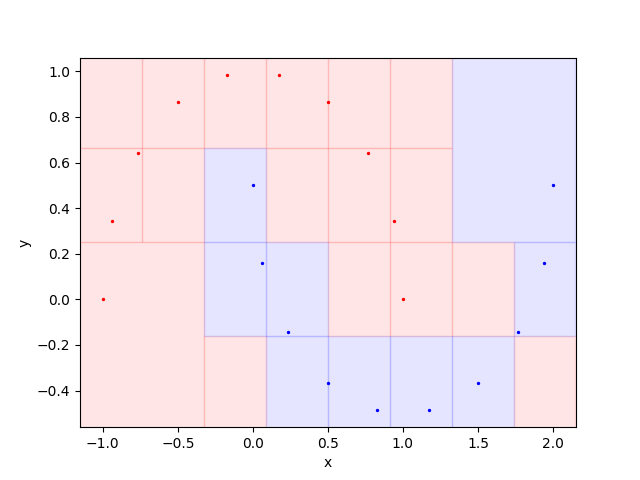
\includegraphics[width=.45\textwidth]{visual20}}\quad
%   \subfloat[][Training Size = 50]{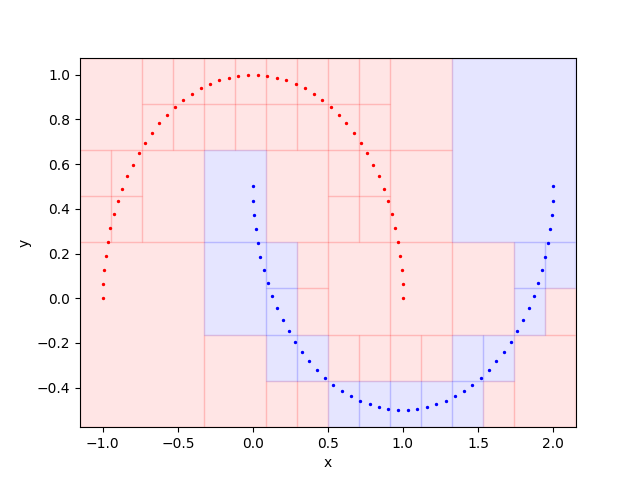
\includegraphics[width=.45\textwidth]{visual50}}\\
%   \subfloat[][Training Size = 500]{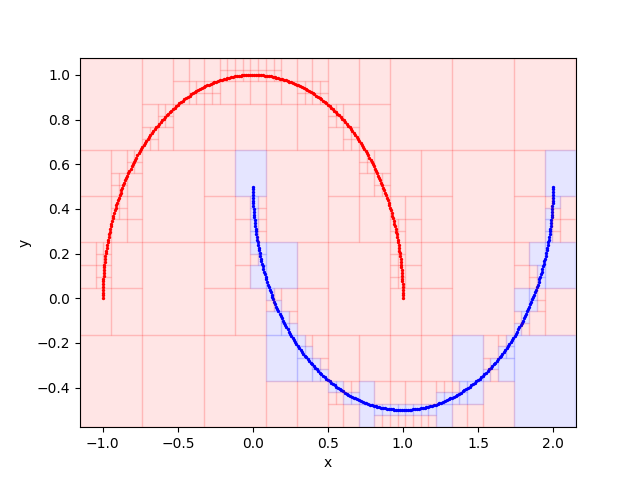
\includegraphics[width=.45\textwidth]{visual500}}\quad
%   \subfloat[][Training Size = 3000]{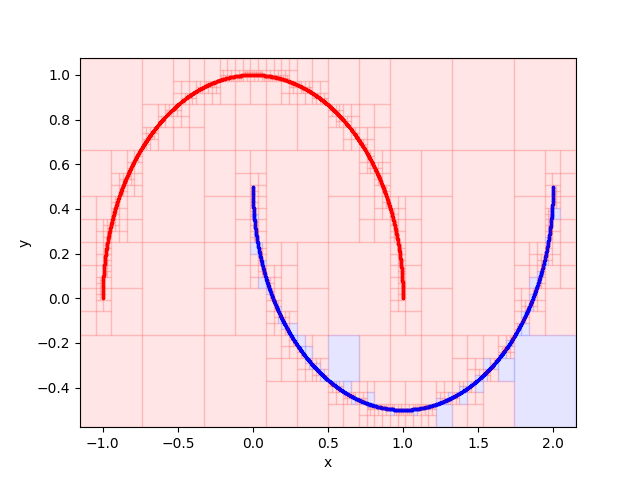
\includegraphics[width=.45\textwidth]{visual3000}}
%\end{center}
%\caption{A visualization of histograms learned with training data sampled from noiseless halfmoon. As training size grows, the histogram classifier becomes increasingly susceptible to adversarial examples in the blue regions.}
%\label{fig:appendix_fig}
%\vskip -0.2in
%\end{figure}

\begin{figure}
\begin{subfigure}{0.45\textwidth}
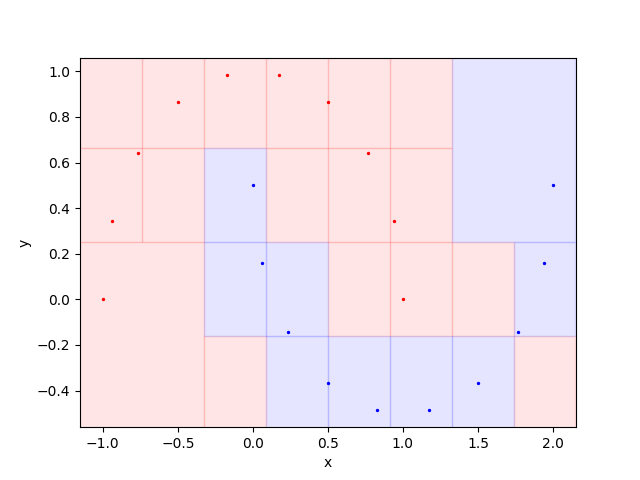
\includegraphics[width=\linewidth]{visual20}
\caption{Training Size = 20} \label{fig:a}
\end{subfigure}\hspace*{\fill}
\begin{subfigure}{0.45\textwidth}
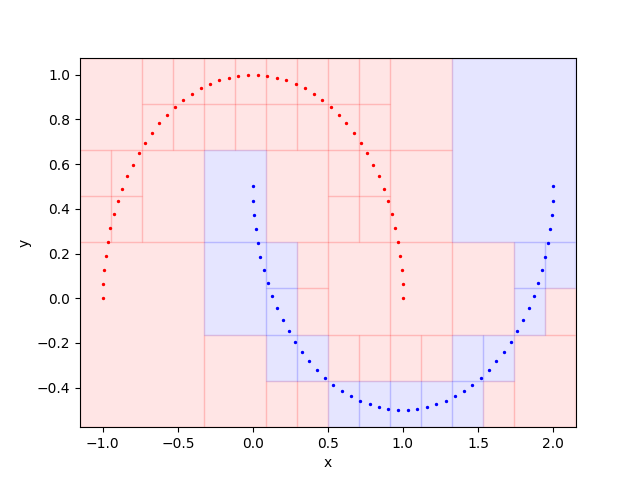
\includegraphics[width=\linewidth]{visual50}
\caption{Training Size = 50} \label{fig:b}
\end{subfigure}

\medskip
\begin{subfigure}{0.45\textwidth}
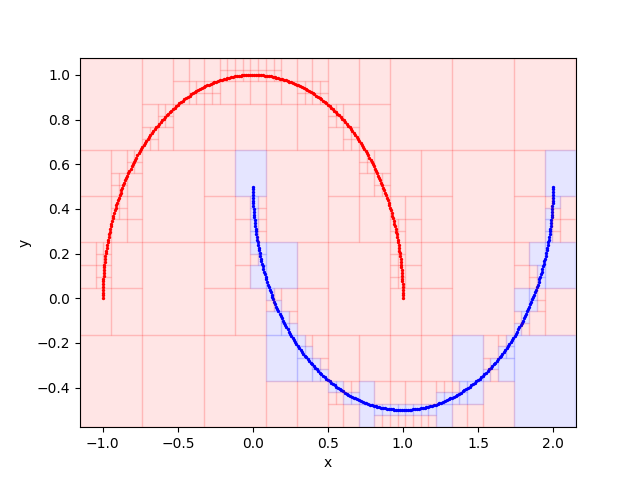
\includegraphics[width=\linewidth]{visual500}
\caption{Training Size = 500} 
\end{subfigure}\hspace*{\fill}
\begin{subfigure}{0.45\textwidth}
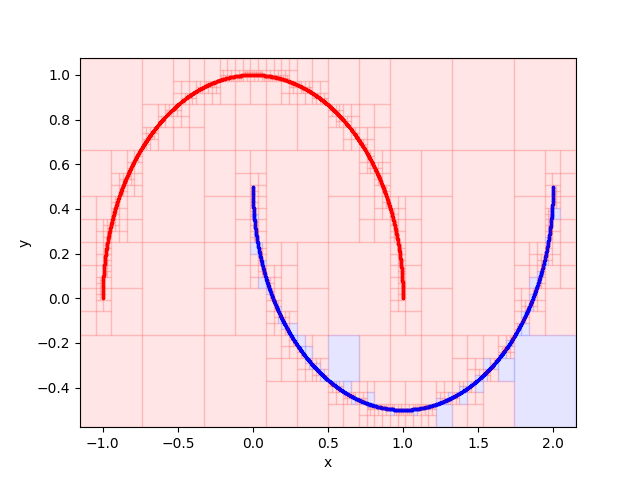
\includegraphics[width=\linewidth]{visual3000}
\caption{Training Size = 3000}
\end{subfigure}
%\caption{Sixth subfigure} \label{fig:f}

\caption{Empirical accuracy/astuteness of different classifiers as a function of training sample size. Accuracy is shown in green, astuteness in purple. Left : Noiseless Setting. Right: Noisy Setting. Top Row: Histogram Classifier, Bottom Row: 1-Nearest Neighbor} \label{fig:appendix_fig}
\end{figure}

\subsection{Optimal attacks against histogram classifiers}

Let $H$ be a histogram classifier, and let $(x,y)$ be any labeled example. Let $r > 0$ be some fixed robustness radius. Recall that an \textit{adversarial example} against $H$ at $(x,y)$ is any $x'$ such that $x' \in B(x,r)$ and $H(x') \neq y$. Note that if $H(x) \neq y$, then $x$ itself is an adversarial example. Conversely, if $H$ is astute at $(x,y)$ with radius $r$, then no adversarial example exists.

For arbitrary classifiers, finding adversarial examples at a given point can be challenging. However, recent work (Yang et. al. 2019) has shown that for non-parametric classifiers, there are tractable methods for doing so. The key insight is that non-parametric classifiers can be construed as a partitioning of input space into convex cells, with each cell having a given label. For example, Figure \ref{fig:appendix_fig} gives a visualization for these cells in a histogram classifier. 

Because these cells are convex, finding an adversarial example for $H$ at $(x,y)$ (here $x$ is a point in $\R^2$, and $y$ is a label) amounts to finding the closest cell $c \in H$ to $x$ such that $H(c) \neq y$. While Yang et. al. (Yang et. al. 2019) presents convex programming algorithms for doing this, the case of histograms in the $\ell_\infty$ metric is much simpler. 

As stated in definition 10, a histogram partitions the input space into hypercubes by iteratively splitting each cube into $2^d$ cubes with half the length. Therefore, the cells of a histogram are all hypercubes of varying sizes. For cell $c$, let $s(c)$ denote the length of the cube that $c$ corresponds to, and let $H(c)$ denote the label $H$ assigns to $c$. The key observation is that $c$ contains an adversarial example for $(x,y)$ if and only if $d(c, x) \leq s(c)/2 + r$, and $H(c) \neq y$. This yields the following algorithm:


Algorithm \ref{alg_hist_attack} was further optimized by utilizing nearest-neighbor type algorithms to find the ``closest" cells to $x$. This was done by grouping cells by their radii, and utilizing a separate nearest-neighbor data structure for all cells of a given radius. 

Although this algorithm doesn't have the same performance metrics as those presented in (Yang et. al. 2019), it was easily sufficient for computing the empirical astuteness for our experiments.

%\begin{algorithm}[tb]
%   \caption{Optimal attack algorithm for Histogram Classifiers}
%   \label{alg_hist_attack}
%\begin{algorithmic}
%   \STATE {\bfseries Input:} Histogram $H$, labeled point $(x,y) \in \R^2 \times \{\pm 1\}$, robustness radius $r$
%   \FOR{cell $c \in H$}
%   \IF{$d(c,x) \leq s(c)/2 + r$ and $H(c) \neq y$}
%   \STATE{Return $c$}
%   \ENDIF
%   \ENDFOR
%\end{algorithmic}
%\end{algorithm}

\begin{algorithm}[H]
    \SetAlgoLined
    {\bfseries Input:} Histogram $H$, labeled point $(x,y) \in \R^2 \times \{\pm 1\}$, robustness radius $r$\;
    
 	\For{cell $c \in H$}{
 		\If{$d(c,x) \leq s(c)/2 + r$ and $H(c) \neq y$}{
 			Return $c$
 		}
 	}
    

\caption{Optimal attack algorithm for Histogram Classifiers}\label{alg_hist_attack}
\end{algorithm}
 
\graphicspath{{./chapters/chapter1/}}
\chapter{Appendix for Chapter 2}

\section{Further Details of Definitions and Theorems}

\subsection{Non-Parametric Classifiers}

In this section, we precisely define weight functions, histogram classifiers and kernel classifiers.

\begin{defn} \label{def:weight_chap_1} 
\cite{devroye96} A \textbf{weight function} $W$ is a non-parametric classifier with the following properties.
\begin{enumerate}
	\item Given input $S = \{(x_1, y_1), (x_2, y_2,), \dots, (x_n, y_n)\} \sim \D^n$, $W$ constructs functions $w_1^S, w_2^S, \dots, w_n^S: \R^d \to [0, 1]$ such that for all $x \in \R^d$, $\sum_1^n w_i^S(x) = 1$. The functions $w_i^S$ are allowed to depend on $x_1, x_2, \dots x_n$ but must be independent of $y_1, y_2, \dots, y_n$. 
	\item $W$ has output $W_S$ defined as \[ W_S(x) = \begin{cases} 
      +1 & \sum_1^n w_i^S(x)y_i > 0 \\
      -1 & \sum_1^n w_i^S(x)y_i \leq 0 \\
   \end{cases}
\]
As a result, $w_i^S(x)$ can be thought of as the weight that $(x_i, y_i)$ has in classifying $x$.
\end{enumerate}
\end{defn}

\begin{defn}
A \textbf{histogram classifier}, $H$, is a non-parametric classification algorithm over $\R^d \times \Y$ that works as follows. For a distribution $\D$ over $\R \times \Y$, $H$ takes $S = \{(x_i, y_i): 1 \leq i \leq n\} \sim \D^n$ as input. Let $k_i$ be a sequence with $\lim_{i \to \infty} k_i = \infty$ and $\lim_{i \to \infty} \frac{k_i}{i} = 0$. $H$ constructs a set of hypercubes $C = \{c_1, c_2, \dots, c_m\}$ as follows:
\begin{enumerate}
	\item Initially $C = \{c\}$, where $S \subset c$.
	\item For $c \in C$, if $c$ contains more than $k_n$ points of $S$, then partition $c$ into $2^d$ equally sized hypercubes, and insert them into $C$.
	\item Repeat step $2$ until all cubes in $C$ have at most $k_n$ points. 
\end{enumerate}
For $x \in \R$ let $c(x)$ denote the unique cell in $C$ containing $x$. If $c(x)$ doesn't exist, then $H_S(x) = -1$ by default. Otherwise, \[ H_S(x) = \begin{cases} 
      +1 & \sum_{x_i \in c(x)} y_i > 0 \\
      -1 & \sum_{x_i \in c(x)}y_i \leq 0 \\
   \end{cases}.
\]
\end{defn}

\begin{defn}
A \textbf{partitioning rule} is a weight function $W$ over $\X \times \Y$ constructed in the following manner. Given $S = \{(x_i, y_i)\} \sim \D^n$, as a function of $\{x_1, \dots, x_n\}$, we partition $\R^d$ into regions with $A(x)$ denoting the region containing $x$.  Then, for any $x \in \R^d$ we have $$w_i^S(x) = \begin{cases}1 & x_i \in A(x) \\ 0 & \text{ otherwise}\end{cases}.$$To achieve $\sum w_i^S(x) = 1$, we can simply normalize weights for any $x$ by $\sum_1^n w_i^S(X)$.
\end{defn}

\begin{defn}
A \textbf{kernel classifier} is a weight function $W$ over $\R^d \times \Y$ constructed from function $K: \R^+ \cup \{0\} \to \R^+$ and some sequence $\{h_n\} \subset \R^+$ in the following manner. Given $S = \{(x_i, y_i)\} \sim \D^n$, we have $$w_i^S(x) = \frac{K(\frac{\d(x, x_i)}{h_n})}{\sum_{j = 1}^n K(\frac{\d(x, x_j)}{h_n})}.$$ Then, as above, $W$ has output \[ W_S(x) = \begin{cases} 
      +1 & \sum_1^n w_i^S(x)y_i > 0 \\
      -1 & \sum_1^n w_i^S(x)y_i \leq 0 \\
   \end{cases}
\]
\end{defn}

\subsection{Splitting Numbers}

We refer to definitions \ref{defn:prob_radius} and \ref{defn:splitting_number}.



The main idea behind splitting numbers is that they allow us to ensure uniform convergence properties over a weight function. To prove neighborhood consistency, it is necessary for a classifier to be correct at \textit{all} points in a given region. Consequently, techniques that consider a single point will be insufficient. The splitting number provides a mechanism for studying entire regions simultaneously. For clarity, we include a quick example in which we bound the splitting number for a given weight function.

\paragraph{Example:} Let $W$ denote any kernel classifier corresponding such that $K: \R_{\geq 0} \to \R_{\geq 0}$ is a decreasing function. For any $S \sim \D^n$, observe that the condition $w_i^S(x) \geq \beta$ precisely corresponds to $\d(x, x_i) \leq \gamma$ for some value of $\gamma$. This is because $w_i^S(x) > w_j^S(x)$ if and only if $\d(x, x_i) < \d(x, x_j)$. Thus, the regions $W_{x, \alpha, \beta}$ correspond to $\{i: \d(x, x_i) \leq \gamma\}$, where $\gamma$ is a positive real number that depends on $x, \alpha, \beta$. These sets precisely correspond to subsets of $S$ that are contained within $B(x, \gamma)$. Since balls have VC dimension at most $d+2$, by  Sauer's lemma, the number of subsets of $S$ that can be obtained in this manner is $O(n^{d+2})$. Therefore, we have that $T(W,S) = O(n^{d+2})\text{ for all }S \sim \D^n.$

\subsection{Stone's Theorem}

\begin{thm}\label{thm_stone_chapter_1}
\cite{Stone77} Let $W$ be weight function over $\R^d \times \Y$. Suppose the following conditions hold for any distribution $\D$ over $\R^d \times \Y$.  Let $X$ be a random variable with distribution $\D_{\R^d}$, and $S = \{(x_1, y_1), (x_2, y_2), \dots, (x_n, y_n)\} \sim \D^n$. All expectations are taken over $X$ and $S$. 

1. There is a constant $c$ such that, for every nonnegative measurable function $f$ satisfying $\mathbb{E} [f(X)] < \infty$, and $\mathbb{E} [\sum_1^n w_i^S(X)f(x_i)] \leq c \mathbb{E} [f(x)].$

2. $\forall a > 0$, $\lim_{n \to \infty} \mathbb{E}[\sum_1^n w_i^S(x)I_{||x_i - X|| > a||}] = 0.$ 

3. $\lim_{n \to \infty} \mathbb{E}[\max_{1 \leq i \leq n} w_i^S(X)] = 0.$

Then $W$ is consistent. 
\end{thm}

\section{Proofs}

\paragraph{Notation:} \begin{itemize}
	\item We let $\d$ denote our distance metric over $\R^d$. For sets $X_1, X_2 \subset \R^d$, we let $\d(X_1, X_2) = \inf_{x_1 \in X_1, x_2 \in X_2} \d(x_1, x_2)$. 
	\item For any $x \in \R^d$, $B(x, a) = \{x: \d(x, x') \leq a\}$.
	\item For any measure over $\R^d$, $\mu$, we let $supp(\mu) = \{x: \mu(B(x,a)) > 0\text{ for all }a > 0\}.$ 
	\item Given some measure $\mu$ over $\R^d$ and some $x \in \R^d$, we let $r_p(x)$ denote the probability radius (Definition \ref{defn:prob_radius}) of $x$ with probability $p$. that is, $r_p(x) = \inf \{r: \mu(B(x,r)) \geq p\}.$
	\item For weight function $W$ and training sample $S$, we let $W_S$ denote the weight function learned by $W$ from $S$.
\end{itemize}

\subsection{Proofs of Theorems \ref{thm:accuracy_margin} and \ref{thm:robust_margin}}

\begin{proof}
(Theorem \ref{thm:accuracy_margin}) Let $\D = (\mu, \eta)$ be a data distribution, and let $\mu^+, \mu^-$ be as described in Definition \ref{defn:includes_mu_plus_and_minus}. Observe that for any $x \in \mu^+$, the Bayes optimal classifier and the \natural\emph{ }Bayes optimal both have the same output, and furthermore the \natural\emph{ }Bayes gives this output (by definition) throughout the entirety of $V_x$, the \natural\emph{ }robustness region of $x$. It follows that the \natural\emph{ }Bayes optimal has optimal astuteness, as desired. 
\end{proof}

\begin{proof}
(Theorem \ref{thm:robust_margin}) Let $\D = (\mu, \eta)$ be a data distribution, and assume towards a contradiction that there exists classifier $f$ which has maximal astuteness with respect towards some set of robustness regions $\U = \{U_x\}$ such that $V_x \subseteq U_x$ for all $x$. The key observation is that because $f$ has maximal astuteness, we must have $f(x) = g(x)$ for almost all points $x \sim \mu$ (where $g$ is the Bayes optimal classifier). Furthermore, for those values of $x$, we must have $g$ be robust at $x$ (meaning it uniformly outputs the same output through $U_x$).

In order for $U_x$ to be strictly larger than $V_x$ for some $x$, it \textit{necessarily} must intersect with $U_{x'}$ for some $x'$ with $g(x') \neq g(x)$, and this is what causes the contradiction: $f$ cannot be astute at both $x$ and $x'$ if they are differently labeled and their robustness regions intersect. 
\end{proof}

\subsection{Proof of Theorem \ref{thm:lower_bound}}

Let $\D = (\mu, \eta)$ be the distribution with $\mu$ being the uniform distribution over $[0, 1]$ and $\eta: [0, 1] \to [0, 1]$ be $\eta(x) = x$. For example, if $(x, y) \sim \D$, then $\Pr[y = 1| x = 0.3] = 0.3$. 

We desire to show that $k_n$-nearest neighbors is not neighborhood consistent with respect to $\D$. We begin with the following key lemma.

\begin{lem}\label{cl:delta}
For any $n > 0$, let $f_n$ denote the $k_n$-nearest neighbor classifier learned from $S \sim \D^n$. There exists some constant $\Delta > 0$ such that for all sufficiently large $n$, with probability at least $\frac{1}{2}$ over $S \sim \D^n$, there exists $x \in [0,1]$ with $\frac{1}{2} - \Delta \leq x \leq \frac{1}{2} - \frac{3\Delta}{4}$ and $f_n(x) = +1$.
\end{lem}

\begin{proof}
Let $C$ be a constant such that $k_n \leq C\log n$ for all $2 \leq n < \infty$. Set $\Delta$ as \begin{equation}\label{eqn:kl}\frac{1}{2}\log_2\frac{1}{1 - 2\Delta} + \frac{1}{2}\log_2\frac{1}{1 + 2\Delta} < \frac{1}{C}.\end{equation} Let $A \subset [0,1]$ denote the interval $[\frac{1}{2} - \Delta, \frac{1}{2} - \frac{3\Delta}{4}]$. For $S \sim \D^n$, with high probability, there exist at least $\frac{\Delta n}{8}$ instances $x_i$ that are in $A$. Let us relabel these $x_i$ as $x_1, x_2, \dots, x_m$ as $$\frac{1}{2} - \Delta \leq x_1 < x_2 < \dots < x_m \leq \frac{1}{2} - \frac{3\Delta}{4}.$$

Next, suppose that for some $i$, at least half of $y_i, y_{i+1}, \dots, y_{i + k_n - 1}$ are $+1$. Then it follows that $f_n(x) = +1$ for $x = \frac{x_{i+k_n} + x_i}{2}$ because the $k_n$ nearest neighbors of $x$ are precisely $x_i, x_{i+1}, \dots x_{i + k_n - 1}$ (as a technical note we make $x$ just slightly smaller to break the tie between $x_i$ and $x_{i + k_n}$). To lower bound the probability that this occurs for some $i$, we partition $y_1, y_2, \dots y_m$ into at least $\frac{m}{2k_n}$ disjoint groups each containing $k_n$ consecutive values of $y_i$. We then bound the probability that each group will have at least $k_n/2$ $+1$s.

Consider any group of $k_n$ $y_i$s. We have that $\Pr[y_i] = +1 = \eta(x_i) = x_i \geq \frac{1}{2} - \Delta$. Since the variables $y_i$ are independent (even conditioning on $x_i$), it follows that the probability that at least half of them are $+1$ is at least  $\Pr[\text{Bin}(k_n, \frac{1}{2} - \Delta) \geq \frac{k_n}{2}].$ For simplicity, assume that $k_n$ is even. Then using a standard lower bound for the tail of a binomial distribution (see, for example, Lemma 4.7.2 of \cite{Ash90}), we have that $$\Pr[\text{Bin}(k_n, \frac{1}{2} - \Delta) \geq \frac{k_n}{2}] \geq \frac{1}{\sqrt{2k_n}}\exp(-k_nD(\frac{1}{2}||(\frac{1}{2} - \Delta)),$$ where $D(\frac{1}{2}||(\frac{1}{2} - \Delta)) =  \frac{1}{2}\log_2\frac{1}{1 - 2\Delta} + \frac{1}{2}\log_2\frac{1}{1 + 2\Delta}$. 

To simplify notation, let $D_\Delta = D(\frac{1}{2}||(\frac{1}{2} - \Delta))$. Then because we have $\frac{m}{2k_n}$ independent groups of $y_i$s, we have that
\begin{equation*}
\begin{split}
\Pr_{S \sim \D^n}[\exists x \in [\frac{1}{2} - \Delta, \frac{1}{2} - \frac{3\Delta}{4}]\text{ s.t. }f_n(x) = +1] &\geq 1 - (1 - \frac{1}{\sqrt{2k_n}}\exp(-k_nD_\Delta))^{\frac{m}{2k_n}} \\
&\geq 1 - \exp(-\frac{m}{2k_n\sqrt{2k_n}}e^{-k_nD_\Delta}) \\
&\geq 1 - \exp(-\frac{n\Delta}{(16C\log n)^{3/2}}e^{-CD_\Delta\log n}),
\end{split}
\end{equation*}
with the inequalities holding because $m \geq \frac{n\Delta}{8}$ and $k_n \leq C \log n$. By equation \ref{eqn:kl}, $CD_\Delta < 1$. Therefore, $\lim_{n \to \infty} \frac{n}{(2C \log n)^{3/2}}e^{-CD_\Delta\log n} = \infty$, which implies that for $n$ sufficiently large, $$\Pr_{S \sim \D^n}[\exists x \in [\frac{1}{2} - \Delta, \frac{1}{2} - \frac{3\Delta}{4}]\text{ s.t. }f_n(x) = +1] \geq \frac{1}{2},$$ as desired.
\end{proof}

We now complete the proof of Theorem \ref{thm:lower_bound}.

\begin{proof}
(Theorem \ref{thm:lower_bound}) Let $\Delta$ be as described in Lemma \ref{cl:delta}, and let $\kappa = \frac{1}{2}$. For all $x < \frac{1}{2}$, we have that $[x, \frac{2x}{3} + \frac{1}{6}] \subseteq V_x^{\kappa}$. This is because we can easily verify that all points inside that interval are closer to $x$ than they are to $\frac{1}{2}$ (and consequently all points in $\mu^+ \cup \mu^{1/2}$) by factor of $2$. It follows that for all $x \in [\frac{1}{2} - \frac{7\Delta}{8}, \frac{1}{2} - \Delta]$, $$[\frac{1}{2} - \Delta, \frac{1}{2} - \frac{3\Delta}{4}] \subseteq V_x^{\kappa}.$$ However, applying Lemma \ref{cl:delta}, we know that with probability at least $\frac{1}{2}$, there exists some point $x' \in [\frac{1}{2} - \Delta, \frac{1}{2} - \frac{3\Delta}{4}]$ such that $f_n(x') = +1$. It follows that with probability at least $\frac{1}{2}$, $f_n$ lacks astuteness at \textit{all} $x \in [\frac{1}{2} - \frac{7\Delta}{8}, \frac{1}{2} - \Delta]$. Since this set of points has total probability mass $\Delta/8$, it follows that with probability at least $\frac{1}{2}$, there is a fixed gap between $A_{\V^\kappa}(f_n, \D)$ and $A(g, \D)$ (as they differ in a region of probability mass at least $\Delta/8$). This implies that $k_n$-nearest neighbors is not \ncons\emph{ }consistent. 
\end{proof}

\subsection{Proof of Theorem \ref{thm:main}}

Let $\D = (\mu, \eta)$ is a distribution over $\R^d \times \{\pm 1\}$. We will use the following notation: let $\D^+ = \{x: \eta(x) > \frac{1}{2}\}$, $\D^- = \{x: \eta(x) < \frac{1}{2}$ and $\D_{1/2} = \{x: \eta(x) = \frac{1}{2}\}$. In particular, we have that $\D^+ = \mu^+, \D^- = \mu^-$ and $\D_{1/2} = \mu^{1/2}$. This notation serve will be convenient throughout this section since it allows us to avoid overloading the symbol $\mu$. 

To show that an algorithm is \ncons\emph{ }consistent with respect to $\D$, we must show that for any $0 < \kappa < 1$, the astuteness with respect to $\V^\kappa$ converges towards the accuracy of the Bayes optimal. To this end, we fix any $0 < \kappa < 1$ and consider $\V^\kappa$. 

For our proofs, it will be useful to have the additional assumption that the robustness regions, $V_x^\kappa$ are \textit{closed}. To obtain this, we let $\U = \{U_x\}$ where $U_x = \overline{V_x^\kappa}$. Each $U_x$ is the closure of the corresponding $V_x^{\kappa}$, and in particular we have $V_x^{\kappa} \subset U_x$. Because of this, it will suffice for us to consider $A_\U$ as opposed to $A_{\V^\kappa}$ since $A_\U(f, \D) \leq A_{\V^\kappa}(f, \D)$ for all classifiers $f$.

We now begin by first proving several useful properties of $\U$ that we will use throughout this entire section. 

\begin{lem}\label{lem:u_is_npr}
The collection of sets $\U = \{U_x\}$ defined as $U_x = \overline{V_x^\kappa}$ satisfies the following properties. 
\begin{enumerate}
	\item $U_x$ is closed for all $x$. 
	\item if $x \in \D^+$, for all $x' \in U_x$, $\d(x, x') < \d(\D^+ \cup \D_{1/2}, x')$.
	\item if $x \in \D^-$, for all $x' \in U_x$, $\d(x, x') < \d(\D^- \cup \D_{1/2}, x')$. 
	\item $U_x = \{x\}$ for all $x \in \D_{1/2}$. 
	\item $U_x$ is bounded for all $x$.
\end{enumerate}
Here $\mu^+, \mu^-, \mu^{1/2}$ are as described in Definition \ref{defn:includes_mu_plus_and_minus}. 
\end{lem}

\begin{proof}
Property (1) is given the by definition, and properties (2), (3) follow from the fact that $\kappa$ is strictly less than $1$. In particular, the distance function $\rho$ is continuous and consequently all limit points of a set have distances that are limits of distances within the set. Property (4) is since $V_x^\kappa = \{x\}$ for all $x \in \D_{1/2}$. 

Finally, property (5) follows from the fact that $\kappa < 1$. As $x$ gets arbitrarily far away from $x$ the ratio of its distance to $x$ with its distance to $\mu^-$ gets arbitrarily close to $1$, and consequently there is some maximum radius $R$ so that $V_x^\kappa \subset B(x, R)$. Since $B(x, R)$ is closed, it follows that $U_x \subset B(x, R)$ as well. 
\end{proof}

Next, fix $W$ as a weight function and $t_n$ is a sequence of positive integers such that the conditions of Theorem \ref{thm:main} hold, that is: 
\begin{enumerate}
	\item $W$ is consistent (with resp. to accuracy) with resp. to $\D$.
	\item For any $0 < p < 1$, $\lim_{n \to \infty} E_{S \sim \D^n} [\sup_{x \in \R^d} \sum_1^n w_i^S(x)1_{\d(x, x_i) > r_p(x)}] = 0.$
	\item $\lim_{n \to \infty} E_{S \sim D^n}[t_n \sup_{x \in \R^d} w_i^S(x)] = 0$.
	\item $\lim_{n \to \infty} E_{S \sim D^n}\frac{\log T(W,S)}{t_n} = 0$.
\end{enumerate}

Finally, we will also make the additional assumption that $\D$ has infinite support. Cases where $\D$ has finite support can be somewhat trivially handled: when the sample size goes to infinity, we will have perfect labels for every point in the support, and consequently condition 2. will ensure that any $x' \in V_x^\kappa$ is labeled according to the label of $x$. 


We also use the following notation. For any classifier $f: \R^d \to \{\pm 1\}$, we let \begin{equation}\label{eqn:cool_sets}\D_f^+ = \{x: f(x' = +1\text{ for all }x' \in U_x\},\text{ and }\D_f^- = \{x: f(x' = -1\text{ for all }x' \in U_x\}.\end{equation} These sets represent the examples that $f$ robustly labels as $+1$ and $-1$ respectively. These sets are useful since they allows us to characterize the astuteness of $f$, which we do with the following lemma.

\begin{lem}\label{lem:conversion_to_measure_thing}
For any classifier $f: \R^d \to \{\pm 1\}$, we have $$A_\U(f, \D) \geq A(g, \D) - \mu(\D^+ \setminus \D_f^+) - \mu(D^- \setminus \D_f^-),$$ where $g$ denotes the Bayes optimal classifier.
\end{lem}

\begin{proof}
By property 4 of Lemma \ref{lem:u_is_npr}, $U_x = \{x\}$ for all $x \in \D_{1/2}$. Consequently, if $x \in \D_{1/2}$, there is a $\frac{1}{2}$ chance that any classifier is astute at $(x,y)$. Using this along with the definition of astuteness, we see that 
\begin{equation*}
\begin{split}
A_\U(f, \D) &= \Pr_{(x,y) \sim \D} [f(x') = y\text{ for all }x' \in U_x] \\
&= \Pr_{(x,y) \sim \D}[y = +1\text{ and }x \in (D^+ \cap D_f^+)] + \Pr_{(x,y) \sim \D}[y = -1\text{ and }x \in (D^- \cap D_f^-)] + \frac{1}{2}\Pr_{(x,y) \sim \D}[x \in \D_{1/2}]
\end{split}
\end{equation*}
However, observe by the definitions of $\D^+, \D^-$ and $\D_{1/2}$ that $$A(g, \D) = \Pr_{(x,y) \sim \D}[y = +1\text{ and }x \in D^+] + \Pr_{(x,y) \sim \D}[y = -1\text{ and }x \in D^-] + \frac{1}{2}\Pr_{(x,y) \sim \D}[x \in \D_{1/2}].$$ Substituting this, we find that 
\begin{equation*}
\begin{split}
A_\U(f, \D) &\geq A(g, \D) - \Pr_{(x,y) \sim \D}[x \in (D^+ \setminus D_f^+)] - \Pr_{(x,y) \sim \D}[x \in (D^- \setminus D_f^-)] \\
&= A(g, \D) - \mu(\D^+ \setminus \D_f^+) - \mu(D^- \setminus \D_f^-),
\end{split}
\end{equation*}
as desired. 
\end{proof}

Lemma \ref{lem:conversion_to_measure_thing} shows that to understand how $W_S$ converges in astuteness, it suffices to understand how the regions $\D_{W_S}^+$ and $\D_{W_S}^-$ converge towards $D^+$ and $D^-$ respectively. This will be our main approach for proving Theorem \ref{thm:main}. Due to the inherent symmetry between $+$ and $-$, we will focus on showing how the region $\D_{W_S}^+$ converges towards $D^+$. The case for $-$ will be analogous. To that end, we have the following key definition. 

\begin{defn}\label{defn:covered}
Let $p, \Delta > 0.$ We say $x \in \D^+$ is $(p, \Delta)$-\textbf{covered} if for all $x' \in U_x$ and for all $x'' \in B(x', r_p(x')) \cap supp(\mu)$, $\eta(x'') > \frac{1}{2} + \Delta.$ Here $r_p$ denotes the probability radius (Definition \ref{defn:prob_radius}). We also let $\D_{p, \Delta}^+$ denote the set of all $x \in \D^+$ that are $(p, \Delta)$-covered. 
\end{defn}

If $x$ is $(p, \Delta)$-covered, it means that for all $x' \in U_x$, there is a set of points with measure $p$ around $x'$ that are both close to $x'$, and likely (with at least probability $\frac{1}{2} + \Delta$) to be labeled as $+1$. Our main idea will be to show that if $x$ is $(p, \Delta)$ covered and $n$ is sufficiently large, $x$ is likely to be in $\D_{W_S}^+$. 

We begin this process by first showing that all $x$ are $(p, \Delta)$-covered for some $p, \Delta$. To do so, it will be useful to have one more piece of notation which we will also use throughout the rest of the section. We let $$\D_{1/2}^{-} = \D^- \cup \D_{1/2} = \supp(\mu) \setminus \D^+.$$ This set will be useful, since Lemma \ref{lem:u_is_npr} implies that for all $x \in \D^+$ and for all $x' \in U_x$, $\d(x, x') < \d(\D_{1/2}^{-}, x').$ We now return to showing that all $x$ are $(p, \Delta$-covered for some $p, \Delta$.

\begin{lem}\label{lem:everything_covered}
For any $x \in \D^+$, there exists $p, \Delta > 0$ such that $x$ is $(p, \Delta)$-covered.
\end{lem}

\begin{proof}
Fix any $x$. Let $f: U_x \to \R$ be the function defined as $f(x') = \d(x', \bad) - \d(x', x)$. Observe that $f$ is continuous. By assumption, $U_x$ is closed and bounded, and consequently must attain its minimum. However, by Lemma \ref{lem:u_is_npr}, we have that $f(x') > 0$ for all $x' \in U_x$. it follows that $\min_{x' \in U_x} f(x') = \gamma$ where $\gamma > 0$.

Next, let $p = \mu(B(x, \gamma/2))$. $p > 0$ since $x \in supp(\mu)$. Observe that for any $x' \in U_x$, $r_p(x') \leq \d(x, x') + \gamma/2$, where, $r_p(x')$ denotes the probability radius of $x'$. This is because $B(x', (\d(x, x') + \gamma/2))$ contains $B(x, \gamma/2)$ which has probability mass $p$. It follows that for any $x' \in U_x$, $\d(x', \bad) \geq r_p(x') + \gamma/2$. Motivated by this observation, let $A$ be the region defined as $$A = \bigcup_{x' \in U_x} B(x', r_p(x')).$$ Then by our earlier observation, we have that $\d(A, \bad) \geq \frac{\gamma}{2}$. Since distance is continuous, it follows that $\d(\overline{A}, \bad) \geq \frac{\gamma}{2}$ as well, where $\overline{A}$ denotes the closure of $A$. 

This means that for any $x'' \in \overline{A} \cap supp(\mu)$, $\eta(x'') > \frac{1}{2}$, since otherwise $\d(\overline{A}, \bad)$ would equal $0$ (as the two sets would literally intersect). Finally, $supp(\mu)$ is a closed set (see Appendix \ref{sec:distribution_details}), and thus $\overline{A} \cap supp(\mu)$ is closed as well. Since $\eta$ is continuous (by assumption from Definition \ref{definition:neighborhood_consistent}), it follows that $\eta$ must maintain its minimum value over $\overline{A} \cap supp(\mu)$. It follows that there exists $2\Delta > 0$ such that $\eta(x'') \geq \frac{1}{2} + 2\Delta > \frac{1}{2} + \Delta$ for all $x'' \in \overline{A} \cap supp(\mu)$. 

Finally, by the definition of $A$, for all $x' \in U_x$, $B(x', r_p(x')) \subset A$. It consequently follows from the definition that $x$ is $(p, \Delta)$-covered, as desired. 
\end{proof}

While the previous lemma show that some $p, \Delta$ cover any $x \in \D^+$, this does not necessarily mean that there are some fixed $p, \Delta$ that cover \textit{all} $x \in \D^+$. Nevertheless, we can show that this is almost true, meaning that there are some $p, \Delta$ that cover \textit{most} $x \in \D^+$. Formally, we have the following lemma.

\begin{lem}\label{lem:most_covered}
For any $\epsilon > 0$, there exists $p, \Delta$ such that $\mu(\D^+ \setminus \D_{p, \Delta}^+) < \epsilon$, where $\D_{p, \Delta}^+$ is as defined in Definition \ref{defn:covered}. 
\end{lem}

\begin{proof}
Observe that if $x$ is $(p, \Delta)$-covered, then it is also $(p', \Delta')$-covered for any $p' < p$ and $\Delta' < \Delta$. This is because $B(x', r_{p'}(x')) \subset B(x', r_p(x))$ and $\frac{1}{2} + \Delta > \frac{1}{2} + \Delta'$. Keeping this in mind, define $$\mathcal{A} = \{\D_{1/i, 1/j}^+: i, j \in \N\}.$$ For any $x \in \D^+$, by Lemma \ref{lem:everything_covered} and our earlier observation, there exists $A \in \mathcal{A}$ such that $x \in A$. It follows that $\cup_{A \in \mathcal{A}} A = \D^+$. By applying Lemma \ref{lem:measure_lemma}, we see that there exists a finite subset of $\mathcal{A}$, $\{A_1, \dots, A_m\}$ such that $$\mu(A_1 \cup \dots \cup A_m\}) > \mu(\D^+) - \epsilon.$$ Let $A_k = \D_{1/i_k, 1/j_k}^+$ for $1 \leq k \leq m$. From our previous observation once again, we see that $\cup A_i \subset \D_{1/I, 1/J}^+$ where  $I = \max(i_k)$ and $J = \max(j_k)$. It follows that setting $p = 1/I$ and $\Delta = 1/J$ suffices. 
\end{proof}

Recall that our overall goal is to show that if $x$ is $(p, \Delta)$-covered, $n$ is sufficiently large, then $x$ is very likely to be in $\D_{W_S}^+$ (defined in equation \ref{eqn:cool_sets}). To do this, we will need to find sufficient conditions on $S$ for $x$ to be in $W_S$. This requires the following definitions, that are related to \textit{splitting numbers} (Definition \ref{defn:splitting_number}). 

\begin{defn}\label{defn:Delta_particular_split_thing}
Let $x \in \R^d$ be a point, and let $S = \{(x_1, y_1), \dots, (x_n, y_n)\}$ be a training set sampled from $\D^n$. For $0 \leq \alpha$, $0 \leq \beta \leq 1$, and $0 < \Delta < \frac{1}{2}$, we define $$W_{x, \alpha, \beta}^{\Delta, S} = \{i: \d(x, x_i) \leq \alpha, w_i^S(x) \geq \beta, \eta(x_i) > \frac{1}{2} + \Delta\}.$$
\end{defn}

\begin{defn}
Let $0 < \Delta < \frac{1}{2}$, and let $S = \{(x_1, y_1), \dots, (x_n, y_n)\}$ be a training set sampled from $\D^n$. Then we let $$W^{\Delta, S} = \{W_{x, \alpha, \beta}^{\Delta, S}: x \in \R^d, 0 \leq \alpha, 0 \leq \beta \leq 1\}.$$
\end{defn}

These convoluted looking sets will be useful for determining the behavior of $W_s$ at some $x \in \D_{p, \Delta}^+$. Broadly speaking, the idea is that if every set of indices $R \subset W^{\Delta, S}$ is relatively well behaved (i.e. the number of $y_i$s that are $+1$ is close to $(|R|(\frac{1}{2} + \Delta)$, the expected amount), then $W_s(x') = +1$ for all $x' \in U_x$. Before showing this, we will need a few more lemmas.

\begin{lem}\label{lem:vc_mimicry}
Fix any $\delta > 0$ and let $0 <  \Delta < \frac{1}{2}$. There exists $N$ such that for all $n > N$ the following holds. With probability $1 - \delta$ over $S \sim \D^n$, for all $R \in W^{\Delta, S}$ with $|R| > t_n$, $\frac{1}{|R|} \sum_{i \in R} y_i \geq \Delta$ 
\end{lem}

\begin{proof}
The key idea is to observe that the set $W^{\Delta, S}$ and the value $T(W, S)$ are completely determined by $\{x_1, \dots, x_n\}$. This is because weight functions choose their weights only through dependence on $x_1, \dots, x_n$. Consequently, we can take the equivalent formulation of first drawing $x_1, \dots, x_n \sim \mu^n$, and then drawing $y_i$ independently according to $y_i = 1$ with probability $\eta(x_1)$ and $0$ with probability $1 - \eta(x_i)$. In particular, we can treat $y_1, \dots, y_n$ as independent from $W^{\Delta, S}$ and $T(W, S)$ conditioning on $x_1, \dots, x_n$. 

Fix any $x_1, \dots, x_n$. First, we see that $|W^{\Delta, S}| \leq T(W, S)$. This is because $W_{x, \alpha, \beta}^{\Delta, S}$ is a subset that is uniquely defined by $W_{x, \alpha, \beta}$ (see Definitions \ref{defn:Delta_particular_split_thing} and \ref{defn:splitting_number}). Second, for any $R \in W^{\Delta, S}$, observe that for all $i \in R$, $y_i$ is a binary variable in $[-1, 1]$ with expected value at least $(\frac{1}{2} + \Delta) - (\frac{1}{2} - \Delta) = 2\Delta$ (again by the definition). It follows that if $|R| \geq t_n$, by Hoeffding's inequality $$\Pr_{y_1 \dots y_n} [\sum_{i \in R} y_i < \Delta] \leq \exp \left( -\frac{2|R|^2\Delta^2}{4|R|} \right) \leq \exp \left( -\frac{t_n\Delta^2}{2} \right).$$ Since there at most $T(W, S)$ sets $R$, it follows that $$\Pr_{y_1 \dots y_n}[\sum_{i \in R} y_i < \Delta\text{ for some }R \in W^{\Delta, S}\text{ with }|R| > t_n] \leq T(W, S)\exp \left( -\frac{t_n\Delta^2}{2} \right).$$ However, by condition 4. of Theorem \ref{thm:main}, it is not difficult to see that this quantity has expectation that tends to $0$ as $n \to \infty$ (unless $T(W, S)$ uniformly equals $1$, but this degenerate case can easily be handled on its own). Thus, for any $\delta > 0$, it follows that there exists $N$ such that for all $n > N$, with probability at least $1 - \frac{\delta}{2}$, $T(W, S)\exp \left( -\frac{t_n\Delta^2}{2} \right) \leq \frac{\delta}{2}$. This value of $N$ consequently suffices for our lemma. 
\end{proof}

We now relate $\D_{W_S}^+$ (Equation \ref{eqn:cool_sets}) to $W^{\Delta, S}$ as well as the conditions of Theorem \ref{thm:main}.

\begin{lem}\label{lem:proving_it_works}
Let $S = \{(x_1, y_1), \dots, (x_n, y_n)\}$ and let $0 < \Delta \leq \frac{1}{2}$ and $0 < p < 1$ such that the following conditions hold. 
\begin{enumerate}
	\item For all $R \in W^{\Delta, S}$ with $|R| > t_n$, $\frac{1}{|R|} \sum_{i \in R} y_i \geq \Delta$. 
	\item $\sup_{x \in \R^d} \sum_1^n w_i^S(x)1_{\d(x, x_i) > r_p(x)} < \frac{\Delta}{5}$.
	\item $t_n\sup_{x \in \R^d} w_i^S(x) < \frac{\Delta}{5}$. 
\end{enumerate}
Then $\D_{p, \Delta}^+ \subseteq \D_{W_S}^+$. 
\end{lem}

\begin{proof}
Let $x \in \D_{p, \Delta}^+$, and let $x' \in U_x$ be arbitrary. It suffices to show that $W_S(x') = +1$ (as $x, x'$ were arbitrarily chosen). From the definition of $W_S$, this is equivalent to showing that $\sum_1^n w_i^S(x')y_i > 0.$ Thus, our strategy will be to lower bound this sum using the conditions given in the lemma statement. 

We first begin by simplifying notation. Since $S$ and $x'$ are both fixed, we use $w_i$ to denote $w_i^S(x')$. Since $n$ is fixed, we will also use $t$ to denote $t_n$. Next, suppose that $|\{x_1, \dots, x_n\} \cap B(x', r_p(x'))| = k$. Without loss of generality, we can rename indices such that $\{x_1, \dots, x_n\} \cap B(x', r_p(x')) \cap B(x', r_p(x')) = \{x_1, \dots, x_k\}$, and $w_1 \geq w_2 \geq \dots \geq w_k.$ 

Let $Y_j = \sum_{i=1}^j y_i$. Our main idea will be to express the sum in terms of these $Y_j$s as follows.  
\begin{equation*}
\begin{split}
\sum_1^n w_iy_i &= \sum_1^k w_iy_i + \sum_{k+1}^n w_iy_i \\
&= w_kY_k + (w_{k-1} - w_k)Y_{k-1} + \dots + (w_{t+1} -w_{t+2})Y_{t+1} + \sum_{i = 1}^t (w_i - w_{t+1})y_i + \sum_{k+1}^n w_iy_i \\
&= \underbrace{w_kY_k + \sum_{i = t+1}^{k-1} (w_i - w_{i+1})Y_i}_{\alpha} + \underbrace{\sum_{i = 1}^t (w_i - w_{t+1})y_i}_\beta + \underbrace{\sum_{k+1}^n w_iy_i}_\tau. 
\end{split}
\end{equation*}

We now bound $\alpha, \beta$ and $\tau$ in terms of $\Delta$ by using the conditions given in the lemma. We begin with $\beta$ and $\tau$, which are considerably easier to handle.

For $\beta$, we have that 
\begin{equation*}
\begin{split}
\beta = \sum_{i=1}^t (w_i - w_{t+1})y_i \geq \sum_{i=1}^t (w_i - w_{t+1})(-1) \geq -tw_1. 
\end{split}
\end{equation*}
By condition 2 of the lemma, we see that $tw_1 < \frac{\Delta}{5}$, which implies that $\beta \geq  -\frac{\Delta}{5}$.

For $\gamma$, we have that $\gamma = \sum_{k+1}^n w_iy_i \geq -\sum_{k+1}^n w_i$. However, for all $k+1 \leq i \leq n$, by definition of $k$, $\d(x', x_i) > r_p(x')$. It follows from condition 3 of the lemma that $\gamma \geq -\frac{\Delta}{5}$.

Finally, we handle $\alpha$. Recall that $x$ is $(p, \Delta)$-covered. It follows that for all $x'' \in supp(\mu) \cap B(x', r_p(x'))$, $\eta(x'') > \frac{1}{2} + \Delta$. Thus, by the definition of $k$, $\eta(x_i) > \frac{1}{2} + \Delta$ for $1 \leq i \leq k$. It follows that if $w_i > w_{i+1}$ or $i = k$, then 
\begin{equation*}
\begin{split}
W_{x', r_p(x'), w_i}^{\Delta, S} &= \{j: \d(x', x_j) \leq r_p(x'), w_j \geq w_i, \eta(x_j) > \frac{1}{2} + \Delta\} \\
&= \{1, \dots, i\}.
\end{split}
\end{equation*}

This implies that $\{1, \dots, i\} \in W^{\Delta, S}$, and consequently that $Y_i \geq i\Delta$, from condition 1 of the lemma. It follows that for all $t < i \leq k$, $(w_{i} - w_{i+1})Y_i \geq i(w_i - w_{i+1})\Delta$, and that $w_kY_k \geq kw_k\Delta$. Substituting these, we find that 
\begin{equation*}
\begin{split}
\alpha &= w_kY_k + \sum_{i = t+1}^{k-1} (w_i - w_{i+1})Y_i \\
&\geq kw_k\Delta + \sum_{i = t + 1}^{k-1} i(w_i - w_{i+1})\Delta \\
&= w_k\Delta + w_{k-1}\Delta + \dots + w_{t+1}\Delta + (t+1)w_{t+1}\Delta. \\
&\geq (1 - \sum_{1^t} w_i - \sum_{k+1}^n w_i)\Delta \\
&\geq (1 - \frac{2\Delta}{5})\Delta \\
&\geq (\frac{4\Delta}{5}),
\end{split}
\end{equation*}
with the last inequalities holding from the arguments given for $\beta$ and $\gamma$ along with the fact that $0 < \Delta \leq  \frac{1}{2}$. Finally, substituting these, we find that $\alpha + \beta + \gamma \geq \frac{4\Delta}{5} - \frac{2\Delta}{5} = \frac{2\Delta}{5} > 0$, as desired. 
\end{proof}

We are now ready to prove the key lemma that forms one half of the main theorem (the other half corresponding to $\D_{W_S}^-$). 

\begin{lem}
Let $\delta, \epsilon > 0$. There exists $N$ such that for all $n > N$, with probability $1 - \delta$ over $S \sim \D^n$, $\mu(\D^+ \setminus \D_{W_S}^+) < \epsilon$. 
\end{lem}

\begin{proof}
First, by Lemma \ref{lem:most_covered}, let $0 < p$ and $0 < \Delta$ be such that $\mu(\D^+ \setminus \D_{p, \Delta}^+) < \epsilon$. By combining Lemma \ref{lem:vc_mimicry}, condition 3 of Theorem \ref{thm:main}, and condition 2 of Theorem \ref{thm:main} respectively,  we see that there exists $N$ such that for all $n > N$, the following hold:
\begin{enumerate}
	\item With probability at least $1 - \frac{\delta}{3}$ over $S \sim \D^n$, for all $R \in W^{\Delta, S}$ with $|R| > t_n$, $\frac{1}{|R|} \sum_{i \in R} y_i \geq \Delta$. 
	\item With probability at least $1 - \frac{\delta}{3}$ over $S \sim \D^n$, $\sup_{x \in \R^d} \sum_1^n w_i^S(x)1_{\d(x, x_i) > r_p(x)} < \frac{\Delta}{5}$.
	\item With probability at least $1 - \frac{\delta}{3}$ over $S \sim \D^n$, $t_n\sup_{x \in \R^d} w_i^S(x) < \frac{\Delta}{5}$. 
\end{enumerate}
By a union bound, this implies that $p, \Delta, S$ satisfy the conditions of Lemma \ref{lem:proving_it_works} with probability at least $1 - \delta$.  Thus, applying the Lemma, we see that with probability $1 - \delta$, $\D_{p, \Delta}^+ \subset \D_{W_S}^+$. This immediately implies our claim. 
\end{proof}

By replicating all of the work in this section for $\D^-$ and $\D_{p, \Delta}^-$, we can similarly show the following: 

\begin{lem}
Let $\delta, \epsilon > 0$. There exists $N$ such that for all $n > N$, with probability $1 - \delta$ over $S \sim \D^n$, $\mu(\D^- \setminus \D_{W_S}^-) < \epsilon$. 
\end{lem}

Combining these two lemmas with Lemma \ref{lem:conversion_to_measure_thing} immediately implies that for all $\delta, \epsilon > 0$, there exists $N$ such that for all $n > N$, with probability $1- \delta$ over $S \sim \D^n$, $$A_\U(W_S, \D) \geq A(g, \D) - \epsilon.$$ Since $V_x^\kappa \subset U_x$ and since $\kappa$ was arbitrary, this implies Theorem \ref{thm:main}, which completes our proof. 

\subsection{Proof of Corollary \ref{cor:nn}}

Recall that $k_n$-nearest neighbors can be interpreted as a weight function, in which $w_i^S(x) = \frac{1}{k_n}$ if $x_i$ is one of the $k_n$ closest points to $x$, and $0$ otherwise. Therefore, it suffices to show that the conditions of Theorem \ref{thm:main} are met. 

We let $W$ denote the weight function associated with $k_n$-nearest neighbors.

\begin{lem}
$W$ is consistent.
\end{lem}

\begin{proof}
It is well known (for example \cite{Dasgupta14}) that $k_n$-nearest neighbors is consistent for $\lim_{n \to \infty} k_n = \infty$ and $\lim_{n \to \infty} \frac{k_n}{n} = 0$. These can easily be verified for our case.
\end{proof}

\begin{lem}
For any $0 < p < 1$, $\lim_{n \to \infty} \E_{S \sim \D^n}[ \sup_{x \in \R^d} \sum_1^n w_i^S(x)1_{\d(x, x_i) > r_p(x)}] = 0.$ 
\end{lem}

\begin{proof}
It suffices to show that for $n$ sufficiently large, all $k_n$-nearest neighbors of $x$ are located inside $B(x, r_p(x))$ for all $x \in \R^d$. We do this by using a VC-dimension type argument to show that all balls $B(x, r)$ contain a number of points from $S \sim \D^n$ that is close to their expectation. 

For $x \in \R^d$ and $r \geq 0$, let $f_{x, r}$ denote the $0-1$ function defined as $f_{x,r}(x') = 1_{x' \in B(x,r)}$. Let $F = \{f_{x, r}: x \in \R^d, r \geq 0\}$ denote the class of all such functions. It is well known that the VC dimension of $F$ is at most $d+2$. 

For $f \in F$, let $\E f$ denote $\E_{(x', y) \sim \D}f(x')$ and $\E_nf$ denote $\frac{1}{n}\sum_1^n f(x_i)$, where $\E_nf$ is defined with respect to some sample $S \sim \D^n$. By the standard generalization result of Vapnik and Chervonenkis (see \cite{Dasgupta07} for a proof), we have that with probability $1- \delta$ over $S \sim \D^n$, \begin{equation}\label{eqn:vc}-\beta_n\sqrt{\E f} \leq \E f - \E_nf \leq \beta_n\sqrt{\E f}\end{equation} holds for all $f \in F$, where $\beta_n = \sqrt{(4/n)((d+2)\ln 2n + \ln(8/\delta)}.$ 

Suppose $n$ is sufficiently large so that $\beta_n \leq \frac{p}{2}$ and $\frac{k_n}{n} < \frac{p}{2}$, and suppose that equation \ref{eqn:vc} holds. Pick any $x \in \R^d$ and consider $f_{x, r}$ where $r > r_p(x)$. This implies $\E f_{x, r} \geq p$. Then by equation \ref{eqn:vc}, we see that $\E_nf \geq \frac{p}{2}$. This implies that all $k_n$ nearest neighbors of $x$ are in the ball $B(x,r)$, and that consequently $\sum_1^n w_i^S(x)1_{\d(x, x_i) > r} = 0$. Because this holds for all $x, r$ with $x \in \R^d$ and $r > r_p(x)$, it follows that equation $2$ implies that $$\sup_{x \in X} \sum_1^n w_i^S(x) 1_{\d(x, x_i) > r_p(x)} = 0.$$ Because equation \ref{eqn:vc} holds with probability at least $1 - \delta$, and $\delta$ can be made arbitrarily small, the desired claim follows. 
\end{proof}

Let $t_n = \sqrt{d k_n\log n}$.

\begin{lem}
 $\lim_{n \to \infty} E_{S \sim D^n}[t_n \sup_{x \in \R^d} w_i^S(x)] = 0$.
\end{lem}

\begin{proof}
Let $S \sim \D^n$. By the definition of $k_n$ nearest neighbors, $\sup_{x \in \R^d}w_i^S(x) = \frac{1}{k_n}$. Therefore, $t_n\sup_{x \in \R^d} w_i^S(x) = \sqrt{\frac{d\log n}{k_n}}$. By assumption 2. of corollary \ref{cor:nn}, $\lim_{n \to \infty} \frac{d \log n}{k_n} = 0$, which implies that $$\lim_{n \to \infty} \E_{S \sim D^n}[t_n\sup_{x \in \R^d} w_i^S(x)] = \lim_{n \to \infty} \sqrt{\frac{d\log n}{k_n}} = \lim_{n \to \infty} \frac{d \log n}{k_n} = 0,$$ as desired.
\end{proof}

\begin{lem}
$\lim_{n \to \infty} E_{S \sim D^n}\frac{\log T(W,S)}{t_n} = 0$.
\end{lem}

\begin{proof}
For $S \sim \D^n$, recall that $T(W, S)$ was defined as $$T(W, S) |\{W_{x, \alpha, \beta}: x \in \R^d, 0 \leq \alpha, 0 \leq \beta \leq 1\}|,$$ where $W_{x, \alpha, \beta}$ denotes $$W_{x, \alpha, \beta} = \{i: \d(x, x_i) \leq \alpha, w_i^S(x) \geq \beta\}.$$ Our goal will to be upper bound $\log T(W, S)$. 

To do so, we first need a tie-breaking mechanism for $k_n$-nearest neighbors. For each $x_i \in S$, we independently sample $z_i \in [0, 1]$ from the uniform distribution. We then tie break based upon the value of $z_i$, i.e. if $\d(x, x_i) = \d(x, x_j)$, we say that $x_i$ is closer to $x$ than $x_j$ if $z_i < z_j$. With probability $1$, no two values $z_i ,z_j$ will be equal, so this ensures that this method always works.

Let $A_{x, \alpha} = \{i: \d(x, x_i) \leq \alpha\}$ and let $B_{x, c} = \{i: z_i \leq c\}.$ The key observation is that for any $\alpha, \beta$, $W_{x, \alpha, \beta} = A_{x, \alpha} \cap B_{x, c}$ for some value of $c$. This can be seen by noting that the nearest neighbors of $x$ are uniquely determined by $\d(x, x_i)$ and $z_i$. Therefore, it suffices to bound $|A = A_{x, \alpha}: x \in \R^d, \alpha \geq 0\}|$ and $|B = \{B_{x, c}: x \in \R^d, c \geq 0\}|$. 

To bound $|A|$, observe that the set of closed balls in $\R^d$ has VC-dimension at most $d+2$. Thus by Sauer's lemma, there are at most $O(n^{d+2}$ subsets of $\{x_1, x_2, \dots, x_n\}$ that can be obtained from closed balls. Thus $|A| \leq O(n^{d+2}$. 

To bound $|B|$, we simply note that $B_{x, c}$ consists of all $i$ for which $z_i \leq c$. Since the $z_i$ can be sorted, there are at most $n+1$ such sets. Thus $|B| \leq n+1$.

Combining this, we see that $T(W, S) \leq |A||B| \leq O(n^{d+3})$. Finally, we see that $$\lim_{n \to \infty} \frac{\log T(W,S)}{t_n} = \lim_{n \to \infty} \frac{O(d\log n)}{\sqrt{k_n d \log n}} = \lim_{n \to \infty} \sqrt{\frac{O(d \log n)}{k_n}} = 0,$$ with the last inequality holding by condition 2. of Corollary \ref{cor:nn}. 

\end{proof}


Finally, we note that Corollary \ref{cor:nn} is an immediate consequence of the previous 4 lemmas as we can simply apply Theorem \ref{thm:main}.

\subsection{Proof of Corollary \ref{cor:kern}}

Let $W$ be a kernel classifier constructed from $K$ and $h_n$ such that the conditions of Corollary \ref{cor:kern} hold: that is, 
\begin{enumerate}
	\item $K: [0, \infty) \to [0, \infty)$ is decreasing and satisfies $\int_{\R^d}K(x)dx < \infty.$
	\item $\lim_{n \to \infty} h_n = 0$ and $\lim_{n \to \infty} nh_n^d = \infty$.
	\item For any $c > 1$, $\lim_{x \to \infty} \frac{K(cx)}{K(x)} = 0$.
	\item For any $x \geq 0$, $\lim_{n \to \infty} \frac{n}{\log n}K(\frac{x}{h_n}) = \infty$.
\end{enumerate}

It suffices to show that the conditions of Theorem \ref{thm:main} are met for $W$. Before doing this, we will describe one additional assumption we make for this case.

\paragraph{Additional Assumption:} We assume that $\D, \U$ are such that there exists some compact set $\X \subset \R^d$ such that for all $x \in supp(\mu)$, $U_x \subset \X$. This is primarily for convenience: observe that any distribution can be approximated arbitrarily closely by distributions satisfying these properties (as each $U_x$ is bounded by assumption). Importantly, because of this, we will note that it is possible for conditions 2. and 3. of Theorem \ref{thm:main} to be relaxed to taking supremums over $\X$ rather than $\R^d$. This is because in our proof, we only ever used these conditions in their restriction to $\bigcup_{x \in supp(\mu)} \bigcup{x' \in U_x} B(x', r_p(x'))$.

Using this assumption, we return to proving the corollary. 

\begin{lem}\label{cl:kern_consistency}
$W$ is consistent with respect to $\D$. 
\end{lem}

\begin{proof}
Condition 1. of Corollary \ref{cor:kern} imply that $K$ is a regular kernel. This together with Condition 2. implies that $W$ is consistent: a proof can be found in \cite{devroye96}. 
\end{proof}

To verify the second condition, it will be useful to have the following definition. 

\begin{defn}\label{defn:probability_epsilon_radius}
For any $p, \epsilon > 0$ and $x \in \X$, define $r_p^\epsilon$ as $$r_p^\epsilon(x) = \sup \{r: \mu(B(x, r)) - \mu(B(x, r_p(x)) \leq \epsilon\}.$$ 
\end{defn}

\begin{lem}\label{cl:rad}
For any $p, \epsilon > 0$, there exists a constant $c_p^\epsilon > 1$ such that $\frac{r_p^\epsilon(x)}{r_p(x)} \geq c_p^{\epsilon}$ for all $x \in \X$, where we set $\frac{r_p^\epsilon(x)}{r_p(x)} = \infty$ if $r_p(x) = 0$. 
\end{lem}

\begin{proof}
The basic idea is to use the fact that $\X$ is compact. Our strategy will be to analyze the behavior of $\frac{r_p^{\epsilon}(x)}{r_p(x)}$ over small balls $B(x_0, r)$ centered around some fixed $x_0$, and then use compactness to pick some finite set of balls $B(x_0, r)$. This must be done carefully because the function $x \to \frac{r_p^\epsilon(x)}{r_p(x)}$ is not necessarily continuous. 

Fix any $x_0 \in \X$. First, observe that $r_p^{\epsilon}(x_0) > r_p(x_0)$. This is because $B(x_0, r_p(x_0)) = \cap_{r > r_p(x_0)} B(x_0,r)$, and consequently $\lim_{r \downarrow r_p(x_0)} \mu(B(x_0, r)) = \mu(B(x_0, r_p(x_))).$ 

Next, define $$s_p^\epsilon(x) = \inf\{r: \mu(B(x, r_p(x)) - \mu(B(x,r)) \leq \epsilon\}.$$ We can similarly show that $r_p(x_0) > s_p^{\epsilon}(x_0)$. 

Finally, define $$r_0 = \frac{1}{3}\min(r_p^{\epsilon}(x_0) - r_p(x_0), r_p(x_0) - s_p^{\epsilon}(x_0)).$$ Consider any $x \in B^o(x_0, r_0)$ where $B^o$ denotes the open ball, and let $\alpha = \d(x_0, x)$. Then we have the following. 
\begin{enumerate}
	\item $r_p(x) \leq r_p(x_0) + \alpha$. This holds because $B(x, r_p(x_0) + \alpha)$ contains $B(x_0, r_p(x_0))$, which has probability mass at least $p$. 
	\item $r_p(x) \geq r_p(x_0) - \alpha$. This holds because if $r_p(x) < r_p(x_0) - \alpha$, then there would exists $r < r_p(x_0)$ such that $\mu(B(x_0, r)) \geq p$ which is a contradiction.
	\item $B(x_0, s_p^{\epsilon}(x_0)) \subset B(x, r_p(x)).$ This is just a consequence of the definition of $r_0$ and the previous observation.
\end{enumerate}
By the definitions of $r_p^\epsilon$ and $s_p^\epsilon$, we see that $\mu(B(x_0, r_p^{\epsilon}(x_0)) - \mu(B(x_0, s_p^\epsilon(x_0)) \leq 2\epsilon$. By the triangle inequality, $B(x, r_p^{\epsilon}(x_0) - \alpha) \subset B(x_0, r_p^\epsilon(x_0))$ and $B(x_0, s_p^{\epsilon}(x_0)) \subset B(x, r_p(x))$. it follows that $$\mu(B(x, r_p^{\epsilon}(x_0) - \alpha)) - \mu(B(x, r_p(x))) \leq 2\epsilon,$$ which implies that $r_p^{2\epsilon}(x) \geq r_p^{\epsilon}(x_0) - \alpha$. Therefore we have the for all $x \in B(x_0, r_0)$, $$\frac{r_p^{2\epsilon}(x) }{r_p(x)} \geq \frac{r_p^{\epsilon}(x_0) - \alpha}{r_p(x_0) + \alpha} \geq \frac{2r_p^\epsilon(x_0) + r_p(x_0)}{r_p^\epsilon(x_0) + 2r_p(x_0)}.$$ Notice that the last expression is a constant that depends only on $x_0$, and moreover, since $r_p^\epsilon(x_0) > r_p(x_0)$, this constant is strictly larger than $1$. Let us denote this as $c(x_0)$. Then we see that $\frac{r_p^{2\epsilon}(x)}{r_p(x)} \geq c(x_0)$ for all $x \in B^o(x_0, r_0)$. 

Finally, observe that $\{B^o(x_0, r_0): x_0 \in \X\}$ forms an open cover of $\X$ and therefore has a finite sub-cover $C$. Therefore, taking $c = \min_{B^o(x_0, r_0) \in C}c(x_0)$, we see that $\frac{r_p^{2\epsilon}(x)}{r_p(x)} \geq c > 1$ for all $x \in \X$. Because $\epsilon$ was arbitrary, the claim holds.
\end{proof}


\begin{lem}\label{cl:kern_radius}
For any $0 < p < 1$, $\lim_{n \to \infty} \E_{S \sim \D^n}[ \sup_{x \in \X} \sum_1^n w_i^S(x)1_{\d(x, x_i) > r_p(x)}] = 0.$ 
\end{lem}


\begin{proof}
Fix $p > 0$, and fix any $\epsilon, \delta > 0$. Pick $n$ sufficiently large so that the following hold.
\begin{enumerate}
	\item Let $c_p^\epsilon$ be as defined from Lemma \ref{cl:rad}. \begin{equation}\label{eqn:ratio}\sup_{x \in \X} \frac{K(c_p^\epsilon r_p(x)/h_n)}{K(r_p(x) / h_n)} < \delta.\end{equation} This is possible because of conditions 2. and 3. of Corollary \ref{cor:kern}, and because the function $x \to r_p(x)$ is continuous.
	\item With probability at least $1 - \delta$ over $S \sim \D^n$, for all $r > 0$, and $x \in \X$, \begin{equation}\label{eqn:uniform_vc}|\mu(B(x,r)) - \frac{1}{n}\sum_1^n 1_{x_i \in B(x, r)}| \leq \epsilon.\end{equation} This is possible because the set of balls $B(x,r)$ has VC dimension at most $d+2$.
\end{enumerate}
We now bound $\E_{S \sim \D^n}[ \sup_{x \in \X} \sum_1^n w_i^S(x)1_{\d(x, x_i) > r_p(x)}]$ by dividing into cases where $S$ satisfies and doesn't satisfy equation \ref{eqn:uniform_vc}. 

Suppose $S$ satisfies equation \ref{eqn:uniform_vc}. By condition 1. of Corollary \ref{cor:kern}, $K$ is decreasing, and by Lemma \ref{cl:rad}, $r_p^\epsilon(x) \geq c_p^\epsilon r_p(x)$. Therefore, we have that for any $x \in \X$,
\begin{equation*}
\begin{split}
\sum_1^n K(\d(x, x_i)/h_n)1_{\d(x, x_i) \geq r_p^\epsilon(x)} &\leq \sum_1^n K(c_p^\epsilon r_p(x)/h_n)\\
&\leq n\delta K(r_p(x)/h_n)),
\end{split}
\end{equation*}
where the second inequality comes from equation \ref{eqn:ratio}. 

Next, by the definition of $r_p^\epsilon(x)$, we have that $\mu(B(x, r_p^\epsilon(x)) - \mu(B(x,r_p(x))) \leq \epsilon$. Therefore, by applying equation \ref{eqn:uniform_vc} two times, we see that for any $x \in \X$ $$\sum_1^n K(\d(x, x_i)/h_n)1_{r_p(x) < \d(x, x_i) \leq r_p^\epsilon(x)} \leq 3n\epsilon K(r_p(x)/h_n).$$ Finally, we have that $$\sum_1^n w_i^S(x) \geq \sum_1^n K(r_p(x)/h_n)1_{\d(x, x_i) \leq r_p(x)} \geq n(p - \epsilon)K(r_p(x)/h_n).$$ Therefore, using all three of our inequalities, we have that for any $x \in \X$
\begin{equation*}
\begin{split}
\sum_1^n w_i^S(x)1_{\d(x, x_i) > r_p(x)} &= \sum_1^n w_i^S(x)1_{\d(x, x_i) > r_p^\epsilon(x)} + \sum_1^n w_i^S(x)1_{r_p^\epsilon \geq \d(x, x_i) > r_p(x)} \\
&= \frac{\sum_1^n K(\d(x, x_i)/h_n)1_{\d(x, x_i) > r_p^\epsilon(x)} + \sum_1^n K(\d(x, x_i)/h_n)1_{r_p^\epsilon \geq \d(x, x_i) > r_p(x)}}{\sum_1^n K(\d(x, x_i)/h_n)} \\
&\leq \frac{ n\delta K(r_p(x)/h_n)) + 3n\epsilon K(r_p(x)/h_n)}{n(p - \epsilon)K(r_p(x)/h_n).} \\
&= \frac{\delta + 3\epsilon}{p - \epsilon}.
\end{split}
\end{equation*}
If $S$ does \textit{not} satisfy equation \ref{eqn:uniform_vc}, then we simply have $\sup_{x \in \X} \sum_1^n w_i^S(x)1_{\d(x, x_i) > r_p(x)} \leq 1$. Combining all of this, we have that 
$$E_{S \sim \D^n} \sum_1^n w_i^S(x)1_{\d(x, x_i) > r_p(x)} \leq \delta(1) + (1-\delta)\frac{\delta + 3\epsilon}{p - \epsilon}.$$ Since $\delta, \epsilon$ can be made arbitrarily small, the result follows. 
\end{proof}

By assumption, $\X$ is compact and therefore has diameter $D < \infty$. Define $$t_ n = \sqrt{n\log nK(\frac{D}{h_n})}\text{ for }1 \leq n < \infty.$$

\begin{lem}\label{cl:kern_tn}
$\lim_{n \to \infty} E_{S \sim D^n}[t_n \sup_{x \in \X} w_i^S(x)] = 0$.
\end{lem}

\begin{proof}
Because $K$ is a decreasing function, we have that $K(D / h_n) \leq K(\d(x, x_i) / h_n) \leq K(0)$. As a result, we have that for any $x \in \X$, 
\begin{equation*}
\begin{split}
t_n\sup_{1 \leq i \leq n}w_i^S(x) &= \frac{t_n\sup_{1 \leq i \leq n}K(\d(x, x_i)/h_n)}{\sum_1^n K(\d(x, x_i)/h_n)} \\
&\leq \frac{t_n K(0)}{nK(D/h_n)} \\
&= K(0)\sqrt{\frac{n\log nK(D/h_n)}{n^2K(D/h_n)^2}} \\
&= K(0)\sqrt{\frac{\log n}{nK(D/h_n)}}.
\end{split}
\end{equation*}
However, by condition 4. of Corollary \ref{cor:kern}, $\lim_{n \to \infty} \frac{n}{\log n}K(D/h_n) = \infty$. Therefore, since the above inequality holds for all $ x\in \X$, we have that $$\lim_{n \to \infty} E_{S \sim D^n}[t_n \sup_{x \in \X} w_i^S(x)] \leq \lim_{n \to \infty} K(0)\sqrt{\frac{\log n}{nK(D/h_n)}} = 0.$$
\end{proof}

\begin{lem}\label{cl:kern_vc}
$\lim_{n \to \infty} E_{S \sim D^n}\frac{\log T(W,S)}{t_n} = 0$.
\end{lem}

\begin{proof}
For $S \sim \D^n$, recall that $T(W, S)$ was defined as $$T(W, S) |\{W_{x, \alpha, \beta}: x \in \X, 0 \leq \alpha, 0 \leq \beta \leq 1\}|,$$ where $W_{x, \alpha, \beta}$ denotes $$W_{x, \alpha, \beta} = \{i: \d(x, x_i) \leq \alpha, w_i^S(x) \geq \beta\}.$$ Our goal will to be upper bound $\log T(W, S)$. 

The key observation is that $W_{x, \alpha, \beta}$ is precisely the set of $x_i$ for which $\d(x, x_i) \leq r$ where $r$ is some threshold. This is because the restriction that $w_i^S(x) \geq \beta$ can be directly translated into $\d(x, x_i) \leq r$ for some value of $r$, as $K$ is a monotonically decreasing function. Thus, $T(W,S)$ is the number of subsets of $S$ that can be obtained by considering the interior of some ball $B(x,r)$ centered at $x$ with radius $r$.

We now observe that the set of closed balls in $\R^d$ has VC-dimension at most $d+2$. Thus by Sauer's lemma, there are at most $O(n^{d+2}$ subsets of $\{x_1, x_2, \dots, x_n\}$ that can be obtained from closed balls. Thus $T(W,S) \leq O(n^{d+2}$. 

Finally, we see that $$\lim_{n \to \infty} \frac{\log T(W,S)}{t_n} = \lim_{n \to \infty} \frac{O(d\log n)}{\sqrt{n\log nK(\frac{D}{h_n})}} \leq \lim_{n \to \infty} \sqrt{\frac{O(d \log n)}{nK(\frac{D}{h_n})}} = 0,$$ with the last equality holding by condition 4. of Corollary \ref{cor:kern}. 
\end{proof}

Finally, we note that Corollary \ref{cor:kern} is an immediate consequences of Lemmas \ref{cl:kern_consistency}, \ref{cl:kern_radius}, \ref{cl:kern_tn}, and \ref{cl:kern_vc}, as we can simply apply Theorem \ref{thm:main}.

\section{Useful Technical Definitions and Lemmas}\label{sec:useful_lemmas}

\begin{lem}\label{lem:measure_lemma}
Let $\mu$ be a measure over $\R^d$, and let $\mathcal{A}$ denote a countable collections of measurable sets $A_i$ such that $\mu(\bigcup_{A \in \mathcal{A}} A) < \infty$. Then for all $\epsilon > 0$, there exists a finite subset of $\mathcal{A}$, $\{A_1, \dots, A_m\}$ such that $$\mu(A_1 \cup A_2 \cup \dots \cup A_m) > \mu(\bigcup_{A \in \mathcal{A}} A) - \epsilon.$$ 
\end{lem}

\begin{proof}
Follows directly from the definition of a measure.
\end{proof}

\subsection{The support of a distribution}\label{sec:distribution_details}

Let $\mu$ be a probability measure over $\R^d$.

\begin{defn}
The \textbf{support} of $\mu$, $\supp(\mu)$, is defined as all $x \in \R^d$ such that for all $r > 0$, $\mu(B(x, r)) > 0$. 
\end{defn}

From this definition, we can show that $supp(\mu)$ is closed.

\begin{lem}
$supp(\mu)$ is closed.
\end{lem}

\begin{proof}
Let $x$ be a point such that $B(x, r) \cap \supp(\mu) \neq \emptyset$ for all $r > 0$. It suffices to show that $x \in supp(\mu)$, as this will imply closure. 

Let $x$ be such a point, and fix $r > 0$. Then there exists $x' \in B(x, r/2)$ such that $x' \in supp(\mu)$. By definition, we see that $\mu(B(x', r/3)) > 0$. However, $B(x', r/3) \subset B(x, r)$ by the triangle inequality. it follows that $\mu(B(x,r)) > 0$. Since $r$ was arbitrary, it follows that $x \in supp(\mu)$.
\end{proof}

\section{Experiment Details}\label{sec:experiment_details}

\begin{figure}
    \centering
        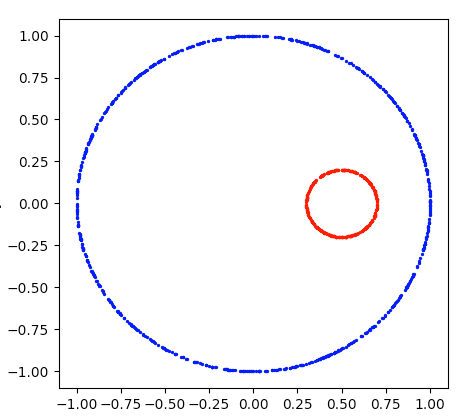
\includegraphics[scale=0.34] {the_distribution.png}
    \caption{Our data distribution $\D = (\mu, \eta)$ with $\mu^+$ shown in blue and $\mu^-$ shown in red. Observe that this simple distribution captures varying distances between the red and blue regions, which necessitates having varying sizes for robustness regions. }
    \label{fig:distribution}
\end{figure}

\paragraph{Data Distribution} Our data distribution $\D = (\mu, \eta)$ is over $\R^2 \times \{\pm 1\}$, and is defined as follows. We let $\mu^+$ consist of a uniform distribution over the circle $x^2 + y^2 = 1$, and $\mu^-$ consist of the uniform distribution over the circle $(x-0.5)^2 + y^2 = 0.04$. The two distributions are weighted so that we draw a point from $\mu^+$ with probability 0.7, and $\mu^-$ with probability $0.3$. Finally, we utilize label noise $0.2$ meaning that the label $y$ matches that given by the Bayes optimal with probability $0.2$. In summary, $\D$ can be described with the following 4 cases:
\begin{enumerate}
	\item With probability $0.7 \times 0.8$, we select $(x,y)$ with $x \in \mu^+$ and $y = +1$.
	\item With probability $0.7 \times 0.2$, we select $(x,y)$ with $x \in \mu^+$ and $y = -1$. 
	\item With probability $0.3 \times 0.8$, we select $(x,y)$ with $x \in \mu^-$ and $y = -1$.
	\item With probability $0.3 \times 0.2$, we select $(x,y)$ with $x \in \mu^-$ and $y = +1$.
\end{enumerate}
We also include a drawing (Figure \ref{fig:distribution}) of the support of $\D$, with the positive portion $\mu^+$ shown in blue and the negative portion, $\mu^-$ shown in red. 

\paragraph{Computing Robustness Regions} 

Recall that in order to measure robustness, we utilize the so-called partial \natural\emph{ }regions $V_x^\kappa$ (Definition \ref{def:partial_nat_region}) for varying values of $\kappa$. In the case of our data distribution $\D$, $V_x^\kappa$ consists of points closer to $x$ by a factor of $\kappa$ than they are to $\mu^-$ (resp. $\mu^+$) when $x \in \mu^+$ (resp. $\mu^-$). To represent a region $V_x^\kappa$, we simply use a function $f$ that verifies whether a given point $x' \in V_x^\kappa$. While this methodology is not sufficient for training general classifiers (for a whole litany of reasons: to begin with it assumes full knowledge of the distribution), it will suffice for our toy synthetic experiments. 


\paragraph{Trained Classifiers} We train two classifiers, both of which are kernel classifiers. 

The first classifier is an exponential kernel classifier with bandwidth function $h_n = \frac{1}{10\sqrt{\log n}}$ and kernel function $K(x) = e^{-x}$. 

The second classifier is a polynomial kernel classifier with bandwidth function $h_n = \frac{1}{10n^{1/3}}$ and kernel function $K(x) = \frac{1}{1 + x^2}$. 

Both of these kernels are regular kernels, and both bandwidths satisfy sufficient conditions for consistency with respect to accuracy.  In other words, both of these classifiers will converge towards the accuracy of the Bayes optimal.

However, the first classifier is selected to satisfy the criterion of Corollary \ref{cor:kern}, whereas the second is not. This distinction is reflected in our experiments. 


\paragraph{Verifying Robustness} To verify the robustness of classifier $f$ at point $x$ (with respect to $V_x^\kappa$), we simply do a grid search with grid parameter 0.01. We grid the entire regions into points with distance at most $0.01$ between them, and then verify that $f$ has the desired value at all of those points. To ensure proper robustness, we also simply verify that $f$ cannot change enough within a distance of $0.01$ by constructing an upper bound on how much $f$ can possibly change. For kernel classifiers, this is simple to do as there is a relatively straightforward upper bound on the gradient of a Kernel classifier.


 
\graphicspath{{./chapters/chapter2/}}
\newcommand\numeq[1]%
  {\stackrel{\scriptscriptstyle(\mkern-1.5mu#1\mkern-1.5mu)}{=}}
 \newcommand\numgeq[1]%
  {\stackrel{\scriptscriptstyle(\mkern-1.5mu#1\mkern-1.5mu)}{\geq}}
  
\def\D{{\mathcal D}}
\def\Pphi{\overline{\Phi}}
\def\F{{\mathcal F}}
\def\N{{\mathcal N}}
%\def\R{{\mathbb R}}
\def\E{{\mathbb E}}
\def\A{\Pi}
\def\B{\Sigma}
\def\diam{\text{diam}}
\def\c{\mathcal L}
\def\l{\ell}
\def\seq{seq}
\def\R{\mathbb{R}}
\def\C{\mathcal C}
\def\p{p}
\def\s{size}
\def\L{\mathcal L}
\def\o{opt}
\def\H{\mathcal H}
\def\calH{\mathcal H}
\def\of{approxCluster}
\def\on{onlineCluster}
\def\R{\mathbb R}
\def\Y{\{\pm 1\}}
\def\U{\mathbb U}
\def\dd{\Delta}
\def\simp{{U\Delta}}
\def\g{g}
\def\rr{R}
\def\f{f}


\chapter{Appendix for Chapter 3}

\section{Expanded summary of \cite{ravikumar20}}\label{sec:appendix_comparison}

In this section, we derive the formulation of Theorem \ref{thm:ravikumar} directly from their results. In particular, their results are not stated in terms of $L_{rob}$ and $L_{std}$, and are instead framed in terms of different parameters. To account for this, we first review these alternative parameters, and then show how the statements in Theorem \ref{thm:ravikumar} can be 

Recall, that \cite{ravikumar20} consider the setting in which the data distribution $\D_{\mu, \Sigma}$ can be characterized as a pair of Gaussians in $\R^d$, $\N(\mu, \Sigma)$ and $\N(-\mu, \Sigma)$, that are symmetric about the origin with each of them representing one label class. They consider robustness measured in any normed metric in $\R^d$, including the $\ell_p$ norm for $p \in [1, \infty]$. 

For any such distribution (and robustness radius $r$), they introduce parameters $s_{rob}(\mu, \Sigma)$ and $s_{std}(\mu, \Sigma)$, which they refer to as the robust and standard signal-to-noise ratios respectively, that are defined as follows:

$$s_{std}(\mu, \Sigma) = 2\sqrt{\mu^t\Sigma^{-1}\mu},$$ $$s_{rob}(\mu, \Sigma) = \min_{||z||_p \leq r} 2\sqrt{(\mu - z)^t\Sigma^{-1}(\mu - z)},$$ where $r$ represents the robustness radius and $\ell_p$ is the distance norm under which adversarial perturbations are measured. 

They then show that these parameters fully characterize the sample complexity for robust and standard learning respectively. They express this through the following results:
\begin{enumerate}
	\item Let $\Phi$ denote the cumulative density function of the standard normal distribution, and let $\overline{\Phi}(x) = 1 - \Phi(x)$. Then for any $\D_{\mu, \Sigma}$, 
		\begin{itemize}
			\item the optimally accurate classifier has standard loss $\Pphi(\frac{1}{2}s_{std})$.
			\item the optimally robust classifier has robust loss $\Pphi(\frac{1}{2}s_{rob})$.
		\end{itemize}		 
	\item For any learning algorithm, there exists some mixture of $\D_{\mu, \Sigma}$ such that the expected robust loss is at least $\Omega(e^{(-\frac{1}{8} + o(1))s_{rob}^2}\frac{d}{n})$.
	\item By contrast, for any distribution $\D_{\mu , \Sigma}$, it is possible to learn a classifier with expected standard loss at most $O(s_{std}e^{-\frac{1}{8}s_{std}^2}\frac{d}{n})$.
	\item Thus, by (2.) and (3.), the gap between the robust sample complexity and the standard complexity can be bounded as $$gap \geq \Omega\left(\frac{e^{(-\frac{1}{8} + o(1))s_{rob}^2}\frac{d}{n}}{s_{std}e^{-\frac{1}{8}s_{std}^2}\frac{d}{n}}\right) \simeq \Omega(e^{\frac{-1}{8}(s_{std}^2 - s_{rob}^2)}).$$ They then qualitatively analyze this gap, and observe that for large values of $\mu$ and large values of $r$, this gap can be arbitrarily large, even as a function of $d$, the dimension.
\end{enumerate}

We now show how to convert (2.), (3.), and (4.) into the statements appearing in Theorem \ref{thm:ravikumar}. As before, let us define $L_{std}$ and $L_{rob}$ as the best possible standard and robust losses for $\D_{\mu , \Sigma}$ respectively. In particular, by (1.), we have $$L_{std} = \Pphi(\frac{1}{2}s_{std}^2),\text{ and }L_{rob} = \Pphi(\frac{1}{2}s_{rob}^2).$$ We now express the bounds in (2.) and (4.) in terms of $L_{std}$ and $L_{rob}$. To do so, we use the well known inequality bounding $\Pphi(x)$ as $$\Omega(\frac{x}{x^2 + 1}e^{-x^2/2}) < \Phi(x) <  O(\frac{e^{-x^2/2}}{x}).$$ Substituting this into (2.) through (4.) imply the following, alternative forms.

\begin{enumerate}
	\item[2.] For any learning algorithm, there exists some mixture of Gaussians, $\D_{\mu, \Sigma}$ such that the expected robust loss is at least $\Omega(L_{rob}\frac{d}{n}).$
	\item[3.] For any distribution $\D_{\mu, \Sigma}$, it is possible to learn a classifier with expected standard loss at most $O(L_{std}\frac{d}{n})$.
	\item[4.] By (2.) and (3.), the gap between robust sample complexity and standard sample complexity can be expressed as $$gap \geq \Omega(\frac{L_{rob}}{L_{std}}).$$
\end{enumerate}

Together, these three statements comprise Theorem \ref{thm:ravikumar}. 

\subsection{The limiting case}

While a core difference between our works is that we consider separated distributions whereas Gaussians are non-separated, we now consider the limiting case in which a pair of Gaussians \textit{appear} separated. To do this, we will consider a case in which $L_{rob}$ is small, and $n \sim O(\frac{1}{L_{rob}})$. In this case, with high probability, a sample of size $n$ will \textit{appear} linearly $r$-separated. Examining the bound in part 1 of Theorem \ref{thm:ravikumar}, we see that their lower bound on the expected robust loss reduces to $O(\frac{1}{n}\frac{d}{n}) = O(\frac{d}{n^2})$, which is significantly weaker than ours (Theorem \ref{thm:lower}). Thus, considering Gaussians that appear linearly $r$-separated does not generalize to the general, linearly $r$-separated case. 

\section{Proof of Theorem \ref{thm:lower}}

We begin by broadly outlining our proof of Theorem \ref{thm:lower}. Let $\A$ be a probability distribution over $\F_{r, \rho}$, and let $A$ be a learning algorithm that returns a linear classifier.

\begin{enumerate}
	\item Sample $\D \sim \A$.
	\item Sample $S \sim \D^n$.
	\item Learn the classifier $A_S$ using algorithm $A$ and training sample $S$.
	\item Evaluate $A_S$ on $\D$. That is, compute $\L_r(A_S, \D)$. 
\end{enumerate}

The basic idea of our proof is to show that for an appropriate choice of $\A$, the overall expected loss of this procedure, $\L_r(A_S, \D)$, satisfies  $$\E_{D \sim \A}[\E_{S \sim \D^n}[\L_r(A_S, \D)]] \geq \Omega(\frac{d}{n}).$$ Our primary method for doing this is switching expectations. In particular, observe that $$\E_{D \sim \A}[\E_{S \sim \D^n}[\L_r(A_S, \D)]] = \E_{S \sim \B}[\E_{\D \sim \Pi|S}[\L_r(A_S, \D)]],$$ where $\B$ denotes the distribution over all $S$ obtained from first sampling $\D \sim \A$ and then sampling $S \sim \D^n$, and $\Pi|S$ denotes the posterior distribution of $\D$ after observing $S$. It then suffices to bound the quantity $\E_{\D \sim \Pi|S}[\L_r(A_S, \D)]$, which is a significantly more tractable problem since we no longer need to deal with any specifics of the Algorithm $A$. In particular, $S$ is fixed in this expectation and consequently $A_S$ is just a fixed linear classifier. This bound subsequently follows from the distribution $\Pi|S$ having enough ``variation" for this expectation to be sufficient large. 

Our proof will have the following main steps, each of which is given its own subsection.

\begin{enumerate}
	\item In section \ref{subsec:constructing_A}, we construct the distribution $\A$, and prove several important properties about it. 
	\item In section \ref{subsec:bound_expectation}, we show that the desired property of $\A$ holds, by bounding $\E_{\D \sim \A|S}[\L_r(A_S, \D)].$
\end{enumerate}


\subsection{Constructing $\A$}\label{subsec:constructing_A}

We let $r$ be a fixed robustness radius, and $\ell_p$ be our norm with which we measure robustness. Our construction of $\A$ is a somewhat technical and lengthy process. We will organize this construction into 4 subsections, outlined here:
\begin{itemize}
	\item In section \ref{subsubsec:D_a}, we define the distribution $\D_a$, characterized by parameter $a \in [0,1]^d$. This forms the basis for constructing $\A$, which will comprise of distributions $\D_a$ for certain choices of $a$. We also show that $\D_a$ is linearly $r$-separated.
	\item In section \ref{subsubsec:dd}, we define the constant $\dd$, which will be essential for specifying which values of parameter $a$ are permissible. 
	\item In section \ref{subsubsec:g1g2}, we define functions $g_1, g_2: [0, \frac{\dd}{3}] \to [0, \frac{\dd}{3}]$ that will be used to construct $\A$. 
	\item In section \ref{subsubsec:finalA}, we finally put together the previous 3 sections and construct $\A$. We also show that any $\D_a \sim \A$ satisfies $\rho(\D_a) \leq C$. 
\end{itemize}

\subsubsection{Defining $\D_a$}\label{subsubsec:D_a}

Let $e_1, e_2, \dots, e_d$ denote the standard normal basis in $\R^d$. Define $v_i = R e_i$ and $u = \frac{\rr}{\sqrt{d}} \sum_1^d e_i$, where $\rr = \frac{9rd^{1/q}}{2\sqrt{d}}$. It will also be convenient to define the following function, which we will frequently use throughout the entirety of the appendix.
\begin{defn}\label{defn:function_f}
For $1 \leq l \leq \infty$, let $\f_l: [0,1]^d \to \R^+$ be the function defined as $$\f_l(a) = \sqrt[l]{\sum_1^d|\frac{1}{\sqrt{d}} + \overline{a} - a_i|^l},$$ where $\overline{a} = \frac{1}{d}\sum_1^d a_i$. For $l = \infty$, we take the convention that $\sqrt[\infty]{\sum_1^d |x_i|^\infty} = \max_{1 \leq i \leq d} |x_i|.$ 
\end{defn}


To define $\D_a$, we first define the concept of a line segment in $\R^d$.
\begin{defn}\label{defn:line_segment}
Let $x_1, x_2 \in \R^d$ be two points. A \textbf{line segment} joining $x_1, x_2$ is defined as one of the following four sets. 
\begin{itemize}
	\item $(x_1, x_2) = \{tx_1 + (1-t)x_t: 0 < t < 1\}$.
	\item $[x_1, x_2) = \{tx_1 + (1-t)x_t: 0 \leq t < 1\}$.
	\item $(x_1, x_2] = \{tx_1 + (1-t)x_t: 0 < t \leq 1\}$.
	\item $[x_1, x_2] = \{tx_1 + (1-t)x_t: 0 \leq t \leq 1\}$.
\end{itemize}
We will always distinguish which set we mean by using the notation above. In all cases, $x_1, x_2$ are said to be the endpoints of the line segment. 
\end{defn}
We now define $\D_a$.
\begin{defn}\label{def:w_dist}
Let $a \in [0,1]^d$ be a vector, and let $\overline{a} = \frac{1}{d}\sum_1^d a_i$. Set $\lambda_a = \frac{r}{\rr}f_q(a)$, where $q$ is the dual norm of $p$. Assume that for all $1 \leq i \leq d$, $a_i > \lambda_a$ (i.e. we only $\D_a$ for $a$ for which this holds). Let $S^-$ and $S^+$ be two sets of $d$ disjoint line segments (as defined in Definition \ref{defn:line_segment}) defined as $$S^- = \{[v_i, v_i + (a_i - \lambda_a)u): 1 \leq i \leq d\},$$ $$S^+ = \{(v_i + (a_i + \lambda_a)u, v_i + u]: 1 \leq i \leq d\}.$$ Then $D_a$ is defined as the probability distribution of random variables $(X,Y)$ where 
\begin{itemize}
	\item $X$ is chosen by the following random procedure. First, sample an arbitrary segment from $S^+ \cup S^-$ with each segment chosen with probability proportional to its $\ell_2$ length. Next, $X$ is selected from the uniform distribution over the chosen line segment. In particular, the probability that $X$ lies on any interval on any line segment contained within $S^+ \cup S^-$ is directly proportional to the length of the interval. 
	\item $Y$ is $-1$ if $X \in \cup S^-$ and $+1$ if $X \in \cup S^+$.
\end{itemize}
\end{defn}

\begin{figure}[h]
\vspace{.3in}
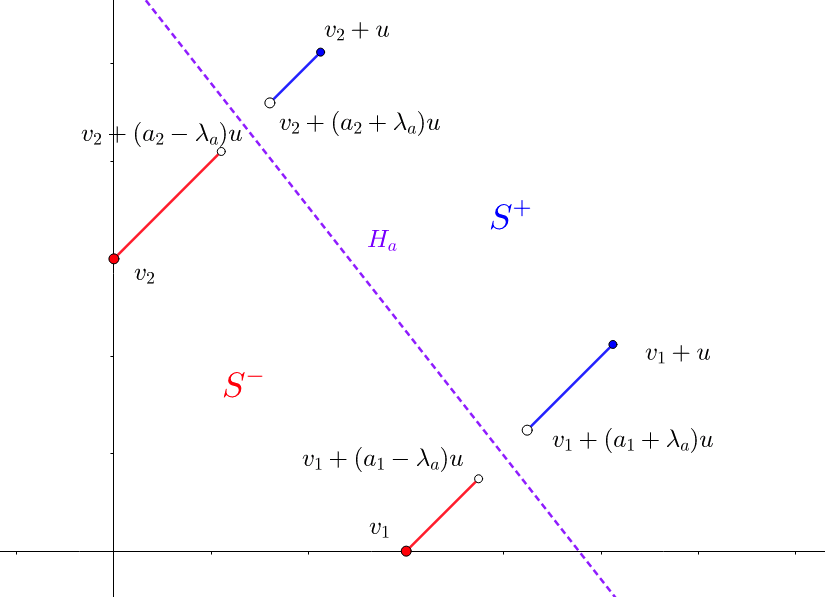
\includegraphics[scale=0.5]{d_a_pic}
\vspace{.3in}
\caption{An illustration of $\D_a$ in two dimensions. $S^-$ is shown in red, and $S^+$ is shown in blue. The decision boundary, $H_a$, of the optimal linear classifier, $f_{w^a, 1}$, is shown in purple. }
\label{fig:d_a_illustration}
\end{figure}

We include an example of such a distribution in Figure \ref{fig:d_a_illustration}. Next, we explicitly compute a linear classifier that linearly $r$-separates $\D_a$.

\begin{defn}\label{def:normal_vector}
Let $a \in [0,1]^d$, and let $\overline{a} = \sum_{i=1}^d a_i.$ Then let $w^a$ be defined as $$w_i^a = \frac{1}{\rr} - \frac{da_i}{\rr\sqrt{d} + d\rr\overline{a}}.$$ 
\end{defn}

\begin{lem}\label{lem:normal_vector_works}
$w^a$ satisfies $\langle w^a, u\rangle = \frac{d}{\sqrt{d} + d\overline{a}}$ and $\langle w^a, v_i + a_iu \rangle = 1,$ for all $1 \leq i \leq d.$ 
\end{lem}

\begin{proof}
By the definitions of $v_i, u$, we have that 
\begin{equation*}
\begin{split}
\langle w^a, u \rangle &= \langle w^a, \frac{1}{\sqrt{d}}\sum_1^d v_i \rangle \\
&= \frac{1}{\sqrt{d}} \sum_1^d Rw_i^a \\
&= \frac{1}{\sqrt{d}} \sum_1^d 1 - \frac{da_i}{\sqrt{d} + d\overline{a}} \\
&= \frac{1}{\sqrt{d}} \sum_1^d \frac{\sqrt{d} + d\overline{a} - da_i}{\sqrt{d} + d\overline{a}} \\
&= \frac{1}{\sqrt{d}} \frac{d\sqrt{d}}{\sqrt{d} + d\overline{a}} = \frac{d}{\sqrt{d} + d\overline{a}},
\end{split}
\end{equation*}
Which proves the first claim. Next, we also have that $\langle w^a, v_i \rangle = Rw_i^a$. Summing these, we get $$Rw_i^a + \frac{da_i}{\sqrt{d} + d\overline{a}} = 1 - \frac{da_i}{\sqrt{d} + d\overline{a}} + \frac{da_i}{\sqrt{d} + d\overline{a}} = 1,$$ as desired. 
\end{proof}

We now prove that $\D_a$ is linearly $r$-separated.

\begin{lem}\label{lem:separation}
$\D_a$ is linearly $r$-separated by the classifier $f_{w_a, 1}$.
\end{lem}

\begin{proof}
Let $H_a$ denote the hyperplane passing through $\{v_i + a_iu: 1 \leq i \leq d\}$. By Lemma \ref{lem:normal_vector_works}, $H_a$ is the decision boundary of $f_{w_a, 1}$.  Referring to Figure \ref{fig:d_a_illustration}, we see that $\cup S^+$ lies entirely above $H_a$ while the set $\cup S^-$ lies entirely below the hyperplane $H_a$, which the classifier $f_{w^a, 1}$ has accuracy $1$ with respect to $\D_a$. It suffices to show that $f_{w^a, 1}$ is robust everywhere. In order to do this, we must show that all points in the support of $\D_a$ have $\ell_p$ distance at least $r$ from $H_a$. 

Fix any $1 \leq i \leq d$. Since the $\ell_p$ distance metric is invariant under translation and scales linearly with dilations, it follows that the point $x_i = v_i + (a_i - \lambda_a)u$ is the closest point on the segment $[v_i, v_i+(a_i - \lambda_a)u)$ to $H_a$. Suppose $x_i$ has distance $D$ under the $\ell_p$ norm to $H_a$. Then the key observation is that the $\ell_p$ ball, $B_p(x_i, D)$, must be tangent to $H_a$. Expressing this as an equation, we have $\max_{z \in B_p(x_i, D)} \langle z, w^a \rangle = 1,$ which can be re-written as $$\max_{||z - x_i||_p \leq D} \langle z - x_i, w^a \rangle = 1 - \langle x_i, w^a \rangle.$$ By Lemma \ref{lem:normal_vector_works} , $\langle w^a, u \rangle = \frac{d}{\sqrt{d} + d\overline{a}}$ and $\langle w^a, v_i + a_iu \rangle = 1$. Substituting this, we see that 
\begin{equation*}
\begin{split}
1 - \langle x_i, w^a \rangle &= 1 - \langle v_i + a_iu - \lambda_a u, w^a \rangle \\
&= 1 - \langle v_i + a_iu, w^a \rangle + \langle \lambda_a u, w^a \rangle \\
&= \langle \lambda_a u, w^a \rangle \\
&= \frac{d\lambda_a}{\sqrt{d} + d\overline{a}}.
\end{split}
\end{equation*}

However, by using the dual norm, we see that $\max_{||z - x_i||_p \leq D} \langle z - x_i, w^a \rangle = D||w^a||_q$. Thus it follows that
\begin{equation*}
\begin{split}
D &= \frac{d\lambda_a}{(\sqrt{d} + d\overline{a})||w^a||_q} \\
&= \frac{d\frac{r}{\rr}f_q(a)}{(\sqrt{d} + d\overline{a})||w^a||_q} \\
&= \frac{d\frac{r}{\rr}\sqrt[q]{\sum_1^d |\frac{1}{\sqrt{d}} + \overline{a} - a_i|^q}}{(\sqrt{d} + d\overline{a})||w^a||_q} \\
&= \frac{r\sqrt[q]{\sum_1^d |\frac{1}{\rr}\frac{\sqrt{d} + d\overline{a} - da_i}{(\sqrt{d} + d\overline{a})}|^q}}{||w^a||_q} \\
&= \frac{r||w^a||_q}{||w^a||_q} = r.
\end{split}
\end{equation*}
We can use an analogous argument holds for $v_i + (a_i + r_a)u$, the closest point to $H_a$ in $S^+$. Thus each point in the support of $D^a$ has distance strictly larger than $r$ (as the endpoints were not included) to $H_a$. Consequently $f_{w^a, 1}$ linearly $r$-separates $D^a$, as desired. 
\end{proof}

\subsubsection{Defining $\dd$}\label{subsubsec:dd}

Now that we have defined $\D_a$, we turn our attention to defining $\A$, which requires us to specify a distribution over valid choices of $a$. In particular, although $\D_a$ is defined for $a \in [0, 1]^d$, we will require a more stringent condition on $a$ for our construction to work. To this end, we begin by defining $\Delta$, a key parameter that characterizes the domain of $a$. To define $\dd$, we use the following lemma.

\begin{lem}\label{lem:dd}
There exists a real number $\dd > 0$ such that for all $l \in \{2, q\}$, and for all $a \in [\frac{1}{2} - \dd, \frac{1}{2} + \dd]^d$, $$||\nabla f_l(a)||_2 \leq \frac{1}{d^2\sqrt{d}},$$ where $f_l$ is as defined in Definition \ref{defn:function_f}.
\end{lem}

\begin{proof}
Since $1 \leq q < \infty$, we see that for both choices of $l$, the function $h_l(x) = (\frac{1}{\sqrt{d}} - x)^l$ is a convex function for $x \in [-\frac{1}{2\sqrt{d}}, \frac{1}{2\sqrt{d}}]$. Thus, if $\sum_1^d x_i = 0$, then by Jensen's inequality, $\sum_1^d h_l(x_i) \geq \sum_1^d h_l(0)$. Applying this, we see that for all $l \in \{2, q\}$ and for all $a \in [\frac{1}{2} - \frac{1}{4\sqrt{d}}, \frac{1}{2} + \frac{1}{4\sqrt{d}}]^d$, 
\begin{equation*}
\begin{split}
f_l(a) &= \sqrt[l]{\sum_1^d |\frac{1}{\sqrt{d}} + \overline{a} - a_i|^l} \\
&= \sqrt[l]{\sum_1^d \left(\frac{1}{\sqrt{d}} + \overline{a} - a_i\right)^l} \\
&= \sqrt[l]{\sum_1^d h_l(a_i - \overline{a})} \\
&\geq \sqrt[l]{\sum_1^d h_l(0)} \\
&= f_l((\frac{1}{2}, \frac{1}{2}, \dots, \frac{1}{2})),
\end{split}
\end{equation*}
with the first equality holding since $\overline{a} - a_i < \frac{1}{\sqrt{d}}$ and the first inequality holding since $\sum_1^d a_i - \overline{a} = 0$. Thus $f_l(a)$ must be locally minimized when $a = (\frac{1}{2}, \frac{1}{2}, \dots, \frac{1}{2})$, and it follows that $$||\nabla f_l(\frac{1}{2}, \frac{1}{2}, \dots, \frac{1}{2})||_2 = 0, \text{ for } l = 2, q.$$ Now observe that the map $H(a) = \max_{l \in \{2, q\}} ||\nabla f_l(a)||_2$ is a continuous map as long as $|a_i - \overline{a}| < \frac{1}{\sqrt{d}}$ for all $1 \leq i \leq d$. Thus there exists an open neighborhood $U$ about $(\frac{1}{2}, \frac{1}{2}, \dots, \frac{1}{2})$ such that $H(a) \leq \frac{1}{d^2\sqrt{d}}$ for all $a \in U$. Taking $\dd$ so that $[\frac{1}{2} - \dd, \frac{1}{2} + \dd]^d \subseteq U$ suffices. 
\end{proof}

\begin{defn}\label{defn:Delta}
Let $\Delta$ be any constant for which Lemma \ref{lem:dd} holds. In particular, $\Delta$ only depends on $\ell_p$, the robustness norm, and $d$, the dimension.
\end{defn}

\subsubsection{Defining $\g_1$ and $\g_2$}\label{subsubsec:g1g2}

In this section, we define functions $\g_1, \g_2: [0, \frac{\Delta}{3}] \to [0, \frac{\Delta}{3}]$ which we will use to specify $\A$. Before defining $\g_1$ and $\g_2$, we will first prove several technical lemmas.

\begin{lem}\label{lem:phi_s}
Let $I \subseteq \R$ be an interval, and $\Phi:I \to \R$ be a strictly convex function.  For any $s \in \R$ and $t \geq 0$, let $\Phi_s(t) = \Phi(s-t) + \Phi(s + t)$. Then $\Phi_s$ is a strictly increasing function.
\end{lem}

\begin{proof}
Fix $s$, and let $0 \leq t_1 < t_2$. Then we see that by Jensen's inequality (for strictly convex functions), $$\Phi(s + t_1) < \frac{(t_2-t_1)\Phi(s+t_2)}{t_1 + t_2} + \frac{2t_1\Phi(s-t_1)}{t_1 + t_2},$$ and $$\Phi(s - t_1) < \frac{(t_2-t_1)\Phi(s-t_2)}{t_1 + t_2} + \frac{2t_1\Phi(s+t_1)}{t_1 + t_2}.$$ Summing these inequalities, we see that 
\begin{equation*}
\begin{split}
\Phi_s(t_1) &= \Phi(s - t_1) + \Phi(s + t_1) \\
&< \frac{(t_2-t_1)\Phi(s+t_2)}{t_1 + t_2} + \frac{2t_1\Phi(s-t_1)}{t_1 + t_2} + \frac{(t_2-t_1)\Phi(s-t_2)}{t_1 + t_2} + \frac{2t_1\Phi(s+t_1)}{t_1 + t_2} \\
&= \frac{t_2 - t_1}{t_1 + t_2}(\Phi(s +t_2) + \Phi(s - t_2)) + \frac{2t_1}{t_1 + t_2}(\Phi(s - t_1) + \Phi(s + t_1)) \\
&= \frac{t_2 - t_1}{t_1 + t_2}\Phi_s(t_2) + \frac{2t_1}{t_1 + t_2}\Phi_s(t_1).
\end{split}
\end{equation*}
Rearranging this yields $\Phi_s(t_1) < \Phi_s(t_2)$, as desired.
\end{proof}

\begin{lem}\label{lem:lipschitz}
Let $I \subseteq \R$ be an interval, $\Phi:I \to \R$ be a strictly convex continuous function, and  $x, y, z \in I$ be real numbers with $x < y < z$. Let $\epsilon >0$ be such that $x - \epsilon \in I$ and $y + \epsilon \leq z - \epsilon$. Then there exist unique $\delta, \gamma >0$ such that the following hold: $$\delta + \gamma = \epsilon,$$ $$\Phi(x-\delta) + \Phi(y + \epsilon) + \Phi(z - \gamma) = \Phi(x) + \Phi(y) + \Phi(z)$$
\end{lem}

\begin{proof}
Fix any $\epsilon$ satisfying the desired conditions, and define $\Theta: [0, \epsilon] \to \R$ as $\Theta(t) = \Phi(x - t) + \Phi(y + \epsilon) + \Phi(z + t - \epsilon)$. Then, utilizing the definition of $\Phi_s$ from Lemma \ref{lem:phi_s}, we see that $$\Theta(t) = \Phi_{\frac{x + z - \epsilon}{2}}(\frac{z - x - \epsilon}{2} + t) + \Phi(y + \epsilon).$$ By Lemma \ref{lem:phi_s}, it follows that $\Theta$ is strictly increasing in $t$, and since $\Phi$ is continuous, so is $\Theta$. Next, we bound $\Theta(0)$ and $\Theta(\epsilon)$ to put us in the configuration to apply the intermediate value theorem. To bound $\Theta(0)$, we have
\begin{equation*}
\begin{split}
\Theta(0) &= \Phi(x) + \Phi(y + \epsilon) + \Phi(z - \epsilon) \\
&= \Phi(x) + \Phi_{\frac{y+z}{2}}(\frac{z - y}{2} - \epsilon) \\
&< \Phi(x) + \Phi_{\frac{y+z}{2}}(\frac{z - y}{2}) \\
&= \Phi(x) + \Phi(y) + \Phi(z),
\end{split}
\end{equation*}
and to bound $\Theta(\epsilon)$, we have 
\begin{equation*}
\begin{split}
\Theta(\epsilon) &= \Phi(x - \epsilon) + \Phi(y + \epsilon) + \Phi(z) \\
&= \Phi_{\frac{x+y}{2}}(\frac{y- x}{2} + \epsilon) + \Phi(z)\\
&> \Phi_{\frac{x+y}{2}}(\frac{y - x}{2}) + \Phi(z) \\
&= \Phi(x) + \Phi(y) + \Phi(z).
\end{split}
\end{equation*}
Together, these equations imply $\Theta(0) < \Phi(x) + \Phi(y) + \Phi(z) < \Theta(\epsilon)$. Since $\Theta$ is strictly increasing and continuous, there exists a unique $\delta \in [0, \epsilon]$ such that $\Theta(\delta) = \Phi(x) + \Phi(y) + \Phi(z)$. Setting $\gamma = \epsilon - \delta$, we see that $$\Theta(\delta) = \Phi(x - \delta) + \Phi(y + \epsilon) + \Phi(z - \gamma) = \Phi(x) + \Phi(y) + \Phi(z),$$ as desired.


\end{proof}



Next, we define a function that will be useful for simplifying notation, both in this section and subsequent ones.

\begin{defn}\label{defn:F_the_function}
Let $\Delta$ be as in definition \ref{defn:Delta}. For $x, y, z \in [0, \frac{\dd}{3}]$, let $$F(x, y, z) = \sqrt[q]{\left(\frac{1}{\sqrt{d}} - x\right)^q + \left(\frac{1}{\sqrt{d}} - \frac{2\Delta}{3} + y\right)^q + \left(\frac{1}{\sqrt{d}} + \frac{2\Delta}{3} + z\right)^q}.$$
\end{defn}

We now define $\g_1, \g_2$.
\begin{cor}\label{cor:lipschitz_maps}
Let $\Delta$ be as in definition \ref{defn:Delta}. There exist $1$-Lipshitz, monotonically non-decreasing functions $\g_1, \g_2: [0, \frac{\dd}{3}] \to [0, \frac{\dd}{3}]$ such that for all $t \in [0, \frac{\dd}{3}]$, $\g_1(t) + \g_2(t) = t$ and $F(t, \g_1(t), \g_2(t)) = F(0, 0, 0)$. 
\end{cor}
\begin{proof}
We have two cases.
\paragraph{Case 1: $1 < q < \infty$:} Let $\Phi: [-\Delta, \Delta] \to \R$ be defined as $\Phi(x) = (\frac{1}{\sqrt{d}} - x)^q$. Since $q > 1$, and $\Delta < \frac{1}{\sqrt{d}}$, $\Phi$ is strictly convex. Observe that $$F(x, y, z)^q = \Phi(x) + \Phi(2\frac{\dd}{3} - y) + \Phi(-2\frac{\dd}{3} - z).$$ Next, fix any $t \in [0, \frac{\Delta}{3}]$. Then observe that $-\frac{2\Delta}{3} \geq -\Delta$ and that $\frac{2\Delta}{3} - t \geq 0 + t$. This puts us in the configuration to apply Lemma \ref{lem:lipschitz}. In particular, there exist unique reals $\delta_t, \gamma_t > 0$ such that $$\delta_t + \gamma_t = t,$$ $$\Phi(-\frac{2\Delta}{3} - \delta_t) + \Phi(t) + \Phi(\frac{2\Delta}{3} - \gamma_t) = \Phi(-\frac{2\Delta}{3}) + \Phi(0) + \Phi(\frac{2\Delta}{3}).$$ We now define $g_1, g_2: [0, \frac{\Delta}{3}] \to [0, \frac{\Delta}{3}]$ as $$g_1(t) = \gamma_t\text{ and }g_2(t) = \delta_t.$$ Then it is clear that $F(0,0,0) = F(t, g_1(t), g_2(t))$ and $g_1(t) + g_2(t)$ (by directly substituting into the equations above). All that remains is to show that $g_1$ and $g_2$ are 1-Lipschitz. 

Fix any $0 \leq t_1 < t_2 \leq \frac{\Delta}{3}$, and let $t_2 - t_1 = \epsilon$. The key idea is to apply Lemma \ref{lem:lipschitz} to $-\frac{2\Delta}{3} - g_2(t_1)<  t_1 < \frac{2\Delta}{3} - g_1(t_1)$ and $\epsilon$. To do so, we first check the conditions of the lemma. 

We have that $$-\frac{2\Delta}{3} - g_2(t_1) - \epsilon \geq -\frac{2\Delta}{3} - t_1 - \epsilon = -\frac{2\Delta}{3} - t_2 \geq -\Delta,$$ and 
\begin{equation*}
\begin{split}
t_1 + \epsilon &= t_2 \\
&\leq \frac{\Delta}{3} \\
&\leq \frac{2\Delta}{3} - t_2 \\
&= \frac{2\Delta}{3} - t_1 - \epsilon \\
&\leq \frac{2\Delta}{3} - g_1(t_1) - \epsilon.
\end{split}
\end{equation*}

Thus $\epsilon$ satisfies the necessary conditions for Lemma \ref{lem:lipschitz}. Since $\Phi$ is strictly convex, by Lemma \ref{lem:lipschitz}, there exist unique $\delta, \gamma > 0$ with $\delta+ \gamma = \epsilon$ such that $$\Phi(-\frac{2\Delta}{3} - g_2(t_1) - \delta) + \Phi(t_1 + \epsilon) + \Phi(\frac{2\Delta}{3} - g_1(t_1) - \gamma) = \Phi(-\frac{2\Delta}{3} - g_2(t_1)) + \Phi(t_1) + \Phi(\frac{2\Delta}{3} - g_1(t_1)).$$ However, by the definition of $g_1, g_2$, we see that both of these quantities are equal to $F(0,0,0)^q$. Moreover, again by the definition of $g_1, g_2$, we also have that $g_1(t_2)$ and $g_2(t_2)$ are the unique real numbers in $[0, \frac{\Delta}{3}$ that satisfy $$\Phi(-\frac{2\Delta}{3} - g_2(t_2)) + \Phi(t_2) + \Phi(\frac{2\Delta}{3}+g_1(t_2)) = F(0,0,0)^q.$$ Thus, it follows that $g_2(t_2) = g_2(t_1) + \delta$ and $g_1(t_2) = g_1(t_1) + \gamma$. However, $t_2 - t_1 = \epsilon$, and $\delta, \gamma < \epsilon$ (since they sum to $\epsilon$). Thus, we see that $|g_1(t_2) - g_1(t_1)| \leq |t_2 - t_1|$ and $|g_2(t_2) - g_2(t_1)| \leq |t_2 - t_1|$. Since $t_1$ and $t_2$ were arbitrary, it follows that $g_1$ and $g_2$ are both $1$-Lipschitz, as desired. 

Finally, since $\delta, \gamma > 0$, it follows that $g_2(t_2) > g_2(t_1)$ and $g_1(t_2) > g_1(t_1)$. Since $t_1, t_2$ were arbitrary, it follows that $g_1, g_2$ are monotonically non-decreasing.

\paragraph{Case 2: $q = 1$} In this case, since $\Delta < \frac{1}{\sqrt{d}}$ (Lemma \ref{lem:dd}), we see that $F(x, y, z) = \frac{3}{\sqrt{d}} + y + z - x$. Setting $\g_1(t) = \g_2(t) = \frac{t}{2}$ suffices, and clearly satisfies the desired properties. 
\end{proof}

\begin{defn}\label{defn:g_1_and_g_2}
Let $\Delta$ be as defined in Definition \ref{defn:Delta}. We let $g_1, g_2: [0, \frac{\Delta}{3}] \to [0, \frac{\Delta}{3}]$ be defined as any function satisfying the conditions of Corollary \ref{cor:lipschitz_maps}.
\end{defn}

\subsubsection{Putting it all together: defining $\A$}\label{subsubsec:finalA}

We are now ready to define $\A$. For convenience, we assume $d$ is a multiple of $3$.
\begin{defn}\label{defn:A}
Let $\Delta, g_1$, and $g_2$ be as defined in Definitions \ref{defn:Delta} and \ref{defn:g_1_and_g_2}. Then $\A$ is defined as the distribution of distributions $\D_a$ where $a$ is a random vector constructed as follows. Let $t_1, t_2, \dots t_{d/3}$ be drawn i.i.d from the uniform distribution over $[0, \frac{\dd}{3}]$. Then for $1 \leq i \leq d/3$, we let
	\begin{itemize}
		\item $a_i = \frac{1}{2} + t_i$.
		\item $a_{i+d/3} = \frac{1}{2} + 2\frac{\dd}{3} - g_1(t_i)$.
		\item $a_{i + 2d/3} = \frac{1}{2} - 2\frac{\dd}{3} - g_2(t_i).$
	\end{itemize}
Together the variables $a_1, a_2, \dots, a_d$ compose $a$. Thus a random distribution $\D \sim \A$ can be constructed by sampling $a$ as above and setting $\D = \D_a$.
\end{defn}

We now show that for all $\D_a \sim \A$, $\lambda_a$ (Definition \ref{def:w_dist}) is constant.

\begin{lem}\label{lem:cons_lambda}
There exists a constant $\Lambda$ such that for all $\D_a \sim \A$, $\lambda_a = \Lambda$. 
\end{lem}

\begin{proof}
Let $\D_a \sim \A$ be arbitrary. By Lemma \ref{cor:lipschitz_maps}, for all $1 \leq i \leq d$, $g_1(t_i) + g_2(t_i) = t_i$. Substituting this, we see that 
\begin{equation*}
\begin{split}
\overline{a} &= \frac{1}{d}\sum_1^d a_i \\
&= \frac{1}{d}\sum_1^{d/3} (\frac{1}{2} + t_i) + (\frac{1}{2} + \frac{2\Delta}{3} - g_1(t_i)) + (\frac{1}{2} - \frac{2\Delta}{3} - g_2(t_i)) \\
&= \frac{1}{d}\sum_1^{d/3} \frac{3}{2} \\
&= \frac{1}{2}.
\end{split}
\end{equation*}

Recall that $\lambda_a = \frac{r}{R}f_q(a) = \frac{r}{R}\sqrt[q]{\sum_1^d |\frac{1}{\sqrt{d}} + \overline{a} - a_i|^q}$. By substituting that $\overline{a} = \frac{1}{2}$ and expressing each $a_i$ in terms of $t_i$, we see that 
\begin{equation*}
\begin{split}
\lambda_a &=  \frac{r}{R}\sqrt[q]{\sum_1^d |\frac{1}{\sqrt{d}} + \overline{a} - a_i|^q}\\
&= \frac{r}{R}\sqrt[q]{\sum_{i=1}^{d/3} \left|\frac{1}{\sqrt{d}} + \frac{1}{2} - (\frac{1}{2} + t_i)\right|^q + \left|\frac{1}{\sqrt{d}} + \frac{1}{2} - \left(\frac{1}{2} + \frac{2\Delta}{3} - g_1(t_i)\right)\right|^q +  \left|\frac{1}{\sqrt{d}} + \frac{1}{2} - \left(\frac{1}{2} - \frac{2\Delta}{3} - g_2(t_i)\right)\right|^q} \\
 &= \frac{r}{R}\sqrt[q]{\sum_1^{d/3} \left|\frac{1}{\sqrt{d}} - t_i\right|^q + \left|\frac{1}{\sqrt{d}} + g_1(t_i) - \frac{2\Delta}{3}\right|^q + \left|\frac{1}{\sqrt{d}} + g_2(t_i) + \frac{2\Delta}{3}\right|^q} \\
&= \frac{r}{R}\sqrt[q]{\sum_1^{d/3}F(t_i, g_1(t_i), g_2(t_i))^q}, \\
\end{split}
\end{equation*}
where $F$ is defined as in Definition \ref{defn:F_the_function}. Next, by Corollary \ref{cor:lipschitz_maps}, $F(t_i, g_1(t_i), g_2(t_i)) = F(0,0,0)$ for all $1 \leq i \leq \frac{d}{3}$. Thus, if we set $\Lambda = \frac{r}{R}(\frac{d}{3})^{1/q}F(0,0,0)$, we have 
\begin{equation*}
\begin{split}
\lambda_a &= \frac{r}{R}\sqrt[q]{\sum_1^{d/3} F(t_i, g_1(t_i), g_2(t_i))^q} \\
&= \frac{r}{R}\sqrt[q]{\sum_1^{d/3}F(0,0,0)^q} \\
&= \frac{r}{R}\sqrt[q]{\frac{d}{3}F(0,0,0)^q} \\
&=  \frac{r}{R}(\frac{d}{3})^{1/q}F(0,0,0) = \Lambda,
\end{split}
\end{equation*}
proving the claim.
\end{proof}

\begin{defn}\label{defn:big_lambda}
We define $\Lambda = \frac{r}{R}(\frac{d}{3})^{1/q}F(0,0,0)$, where $F$ is defined as in Definition \ref{defn:F_the_function}.
\end{defn}

Next, we compute upper and lower bounds on $\Lambda$, both of which will be useful for subsequent lemmas. 
\begin{lem}\label{lem:lambda_bounds}
$\frac{1}{9} < \Lambda < \frac{1}{3}$. 
\end{lem}

\begin{proof}
By definition, $\Lambda = \frac{d}{3}^{1/q}F(0, 0, 0)$. Substituting the definition of $f$, we see that  $F(0, 0, 0) = \sqrt[q]{|\frac{1}{\sqrt{d}}|^q + |\frac{1}{\sqrt{d}} - \frac{2\Delta}{3}|^q + |\frac{1}{\sqrt{d}} + \frac{2\Delta}{3}|^q},$ and consequently, $$3^{1/q}|\frac{1}{\sqrt{d}} - \frac{2\Delta}{3}| \leq F(0, 0, 0) \leq 3^{1/q}|\frac{1}{\sqrt{d}} + \frac{2\Delta}{3}|.$$ By definition, $\frac{2\Delta}{3} < \frac{1}{2\sqrt{d}}$. It follows that $$\frac{r}{R}\frac{d^{1/q}}{2\sqrt{d}} < \Lambda < \frac{r}{R}\frac{3d^{1/q}}{2\sqrt{d}}.$$ Finally, since $\frac{r}{R} = \frac{2\sqrt{d}}{9d^{1/q}}$, substituting this yields $\frac{1}{9} < \Lambda < \frac{1}{3}$, as desired.
\end{proof}

Next, we show that for all $\D_a \in \A$, the aspect ratio (Definition \ref{defn:aspect_ratio}), $\rho(\D_a)$, is bounded by a constant.

\begin{lem}\label{lem:large_margin}
For all $\D_a \in \A$, we have $\rho(\D_a) \leq 18\sqrt{3}$. 
\end{lem}

\begin{proof}
We first bound the $\ell_2$ margin, $\gamma(\D_a)$ (Definition \ref{defn:margin}). Recall that the margin, $\gamma(\D_a)$ is described as the largest possible $\ell_2$ distance from the support of $\D_a$ to the decision boundary of a linear classifier. Thus, we can lower bound $\gamma(\D_a)$ by computing the distance from the support of $\D_a$ to $H_a$, the decision boundary of $f_{w^a, 1}$ (Definition \ref{def:normal_vector}).

By referring to Figure \ref{fig:d_a_illustration} (in Section \ref{subsubsec:D_a}), it becomes clear that the closest point (under the $\ell_2$ margin) from $S^-$ to $H_a$ is the point $v_i + (a_i - \lambda_a)u$, for some value of $i$. Thus it suffices to compute the $\ell_2$ distance from this point to the plane $H_a$. 

Recall that by Lemma \ref{lem:normal_vector_works}, the point $v_i + a_iu$ satisfies $\langle w^a, v_i + a_iu \rangle = 1$, and consequently must lie on the hyperplane $H_a$. Let $D$ denote the $\ell_2$ distance from $v_i + (a_i - \lambda_a)u$ to $H_a$. Since $w^a$ is the normal vector to $H_a$, it follows that
\begin{equation*}
\begin{split}
D &= \langle v_i + a_iu - (v_i + (a_i - \lambda_a)u), \frac{w^a}{||w^a||_2} \rangle \\
&= \frac{\langle \lambda_a u, w^a \rangle}{||w^a||_2} \\
&\numeq{1} \frac{\langle \Lambda u, w^a \rangle}{||w^a||_2} \\
&\numeq{2} \frac{\Lambda \frac{d}{\sqrt{d} + d\overline{a}}}{||w^a||_2}  \\
&\numeq{3} \frac{\Lambda \frac{d}{\sqrt{d} + d\overline{a}}}{\sqrt{\sum_1^d \left(\frac{\sqrt{d} + d\overline{a} - da_i}{R(\sqrt{d} + d\overline{a}}\right)^2}} \\
&= \frac{R\Lambda}{\sqrt{\sum_1^d (\frac{1}{\sqrt{d}} + \overline{a} - a_i)^2}} \\
&\numeq{4} \frac{R\Lambda}{f_2(a)}.
\end{split}
\end{equation*}
Here, (1) holds by Lemma \ref{lem:cons_lambda}, (2) holds by Lemma \ref{lem:normal_vector_works}, (3) holds by Definition \ref{def:normal_vector}, and (4) holds by Definition \ref{defn:function_f}.

Next, observe that since $\D_a \sim \A$, we must have $a \in [\frac{1}{2} - \Delta, \frac{1}{2} + \Delta]^d$. Thus it follows that $||a - (\frac{1}{2}, \frac{1}{2}, \dots, \frac{1}{2})||_2 \leq \Delta\sqrt{d}$. However, by applying Lemma \ref{lem:dd}, we also see that $f_2$ is $\frac{1}{d^2\sqrt{d}}$-Lipschitz over $[\frac{1}{2} - \Delta, \frac{1}{2} + \Delta]^d$. Thus, it follows that $$f_2(a) \leq f_2(\frac{1}{2}, \frac{1}{2}, \dots, \frac{1}{2}) + \Delta\sqrt{d} \frac{1}{d^2\sqrt{d}} \leq 2,$$ with the latter inequality holding from the definition of $\Delta$. 

Substituting this and applying Lemma \ref{lem:lambda_bounds}, we see that $$\gamma(\D_a) \geq \frac{R\Lambda}{2} \geq \frac{R}{18}.$$ Next, to bound the aspect ratio, $\rho(\D_a)$, we must also bound the $\ell_2$ diameter of $\D_a$. However, the $\ell_s$ diameter of $\D_a$ is $R\sqrt{3}$, since it is the distance from $v_i + u$ to $v_j$ for $i \neq j$. Thus, it follows that $$\rho(\D_a) = \frac{diam_2(\D_a)}{\gamma(\D_a)} \leq \frac{R\sqrt{3}}{R/18} = 18\sqrt{3},$$ as desired. 
\end{proof}

Note that a tighter analysis (and selection of $\Delta$) can give a smaller bound for $\rho(\D_a)$, but the most important fact is that $\rho(\D_a) = O(1)$. 

\subsection{Bounding the expected robust loss}\label{subsec:bound_expectation}

In this section, we finally prove our lower bound, Theorem \ref{thm:lower}. This will require a few important steps, which we have separated into the following subsections. 
\begin{itemize}
	\item In section \ref{subsubsec:loss_bounding}, we give a useful lower bound for the loss $\L_r(f, \D_a)$ where $f$ is an arbitrary linear classifier. 
	\item In section \ref{subsubsec:posterior}, we give an explicit computation for the posterior distribution $\A|S$ where $S \sim \D_a^n$ is the observed training sample. 
	\item Finally, in section \ref{subsubsec:proof}, we present the proof of Theorem \ref{thm:lower}.
\end{itemize}

\subsubsection{Bounding the loss $\L_r(f, \D_a)$}\label{subsubsec:loss_bounding}

In this section, we find a lower bound on the loss $\L_r(f, \D_a)$ where $f$ is a linear classifier. We begin by first restricting $f$ to be in the set of classifiers $$f \in \{f_{w^b, 1}: b \in [0, 1]^d\},$$ where $w^b$ is as defined in Definition \ref{def:normal_vector}. These are precisely the classifiers that have a decision boundary that passes through some point on every line segment in $\{[v_i, v_i + u]: 1 \leq i \leq d\}$. We are able to only consider these classifiers since all other linear classifiers clearly have a very high loss with respect to $\D_a$ as they necessarily misclassify at least half the points on the line segment $[v_i, v_i + u]$ for some value of $i$. 

We now find an initial lower bound on $\L_r(f_{w^b, 1}, \D_a)$.

\begin{lem}\label{lem:loss_bound_general}
Fix any $\D_a \in \A$, and let $b \in [0,1]^d$ be arbitrary. Let $w^b$ be the vector defined as in Definition \ref{def:normal_vector}, and $\lambda_b = \frac{r}{\rr}\f_q(b)$ where $f$ is as defined in Definition \ref{defn:function_f}. Then $$\L_r(f_{w^b, 1}, \D_a) \geq \frac{d(\lambda_b - \lambda_a) + \sum_1^d|a_i - b_i|}{d - 2d\Lambda}.$$ 
\end{lem}

\begin{proof}
By Lemma \ref{lem:separation}, $f_{w^b, 1}$ precisely $r$-separates $\D_b$. This implies that for all $1 \leq i \leq d$,
$$f_{w^b, 1}(x) = \begin{cases} 1 & x \in (v_i + (b_i + \lambda_b)u, v_i + u] \\-1 & x \in [v_i, v_i + (b_i - \lambda_b)u) \\ \text{not robust} & x \in [v_i + (b_i - \lambda_b)u, v_i + (b_i + \lambda_b)u] \end{cases}.$$ Without loss of generality, suppose that $b_i \geq a_i$. The key observation is that for all $1 \leq i \leq d$, if $x \in [v_i + (a_i + \lambda_a)u, v_i + (b_i + \lambda_b)u]$, then $f_{w^b, 1}(x) = -1$ for $f_{w^b, 1}$ is not robust at $x$. In both cases, we see that $f_{w^b, 1}$ is either inaccurate or not robust for all points in $[v_i + (a_i + \lambda_a)u, v_i + (b_i + \lambda_b)u]$. 

This interval has $\ell_2$ length at least $(|a_i - b_i| + (\lambda_b - \lambda_a))||u||_2$. Note that in the case that $a_i \leq b_i$ we can get an identical expression. Thus,  combining this for all $i$, we see that $f_{w^b, 1}$ is either inaccurate or not robust for a total length of $[d(\lambda_b - \lambda_a) + \sum_1^d |a_i - b_i|]||u||_2$. Dividing by the total length of the support of $\D_a$, we find that
\begin{equation*}
\begin{split}
\L_r(f_{w^b, 1}, \D_a) &\geq \frac{[d(\lambda_b - \lambda_a) + \sum_1^d |a_i - b_i|]||u||_2}{\sum_1^d ||[v_i, v_i + (a_i - \lambda_a)u) + (v_i + (a_i + \lambda_a)u, v_i + u]||_2} \\
&= \frac{[d(\lambda_b - \lambda_a) + \sum_1^d |a_i - b_i|]||u||_2}{\sum_1^d ||u_2||(1 - 2\lambda_a)} \\
&= \frac{d(\lambda_b - \lambda_a) + \sum_1^d |a_i - b_i|}{d(1 - 2\lambda_a)} \\
&= \frac{d(\lambda_b - \lambda_a) + \sum_1^d |a_i - b_i|}{d - 2d\Lambda},
\end{split}
\end{equation*}
with the last equality holding since by Lemma \ref{lem:cons_lambda}, $\lambda_a = \Lambda$. 
\end{proof}

\begin{lem}\label{lem:loss_bound_clever}
For all $\D_a \in \A$ and $b \in [0,1]^d$, $d(\lambda_a - \lambda_b) \leq \frac{1}{2}\sum_1^d |a_i - b_i|.$ 
\end{lem}

\begin{proof}
We have two cases.
\paragraph{Case 1:} $b \in [\frac{1}{2} - \Delta, \frac{1}{2} + \Delta]^d$.

Observe that $\lambda_b = \frac{r}{R}f_q(b)$ and $\lambda_a = \frac{r}{R}f_q(a)$. By Lemma \ref{lem:dd}, we see that $f_q$ is $\frac{1}{d^2\sqrt{d}}$-Lipschitz over the domain $[\frac{1}{2} - \Delta, \frac{1}{2} + \Delta]^d$. It follows that
\begin{equation*}
\begin{split}
\lambda_a - \lambda_b &= \frac{r}{R}(f_q(a) - f_q(b)) \\
&\leq \frac{r}{R}||a - b||_2\frac{1}{d^2\sqrt{d}} \\
&= \frac{2\sqrt{d}}{9d^{1/q}}||a - b||_2\frac{1}{d^2\sqrt{d}} \\
&< \frac{||a - b||_1}{2d},
\end{split}
\end{equation*}
with the last inequality following since the $\ell_2$ norm is smaller than the $\ell_1$ norm. Rearranging this gives the statement of the Lemma as desired.

\paragraph{Case 2: } $b \notin [\frac{1}{2} - \Delta, \frac{1}{2} + \Delta]^d$.

The main idea in this case will be to find $b' \in [\frac{1}{2} - \Delta, \frac{1}{2} + \Delta]^d$ such that $\lambda_b \geq \lambda_{b'}$ and such that $||b' - a||_1 \leq ||b - a||_1$. We will then apply Case 1 to get the desired result.

Without loss of generality, assume that $b_1 \geq b_2 \geq \dots \geq b_d$, and that $b_1, b_2, \dots b_k > \frac{1}{2} + \Delta$, $b_{k+1}, \dots, b_l \in [\frac{1}{2} - \Delta, \frac{1}{2} + \Delta]$, and $b_{l+1}, \dots b_d < \frac{1}{2} - \Delta$ for some values of $k$ and $l$. 

We will construct $b'$ in four steps. In each of these steps, we will change the values of $b_i$ such that neither $||a - b||_1$ nor $\lambda_b$ are increased. At each step, we let $b_i$ refer to its value at the end of the previous step. 


Finally, for reference, recall that $$\lambda_b = \frac{r}{R}f_q(b) = \frac{r}{R}\sqrt[q]{\sum_1^d |\frac{1}{\sqrt{d}} + \overline{b} - b_i|^q}.$$

\paragraph{Step 1:} We set $$b_i \leftarrow  \begin{cases} \frac{1}{k}\sum_{j=1}^k b_j & 1 \leq i \leq k \\b_i & k+1 \leq i \leq l \\  \frac{1}{d-l}\sum_{j=l+1}^d b_j& l+1 \leq i \leq d \end{cases}.$$ Since $a \in [\frac{1}{2} - \Delta, \frac{1}{2} + \Delta]^d$, we see that these operations do not change $||a - b||_1$, as $\sum_1^k |b_i - a_i| = \sum_1^k b_i - a_i$ and $\sum_{l+1}^d |b_i - a_i| = \sum_1^k a_i - b_i$. Also, observe that this operation preserves $\overline{b}$, and consequently since the function $f(x) = |\frac{1}{\sqrt{d}} + \overline{b} - x|^q$ is convex, we see that by Jensen's inequality that $\lambda_b$ is not increased by this operation.

\paragraph{Step 2:} Let $\beta = \sum_1^k(b_i - \frac{1}{2} - \Delta) - \sum_{l+1}^d (\frac{1}{2} - \Delta - b_i)$. Then we set $$b_i \leftarrow  \begin{cases} \begin{cases} \frac{1}{2} + \Delta + \frac{\beta}{k} & 1 \leq i \leq k \\ b_i & k+1 \leq i \leq l \\ \frac{1}{2} - \Delta & l+1 \leq i \leq d \end{cases} & \beta \geq 0 \\\begin{cases} \frac{1}{2} + \Delta & 1 \leq i \leq k \\ b_i & k+1 \leq i \leq l \\ \frac{1}{2} - \Delta + \frac{\beta}{d - l} & l+1 \leq i \leq d \end{cases} & \beta < 0\end{cases}.$$

Observe that this operation cannot increase $||a - b||_1$, since it doesn't increase $|a_i - b_i|$ for any value of $i$. Furthermore, this operation also does not change $\overline{b}$, and a similar convexity argument on the function $f(x) = |\frac{1}{\sqrt{d}} + \overline{b} - x|^q$ can show that this does not increase $\lambda_b$. 

Finally, if $\beta = 0$, we set $b' = b$, since we have reached a state such that $b \in [\frac{1}{2} - \Delta, \frac{1}{2} + \Delta]^d$. 

\paragraph{Step 3a:} We run this step if $\beta > 0$. Let $\alpha = \frac{\sum_{k+1}^d (\frac{1}{2} + \Delta - b_i)}{\beta}$. We then set  $$b_i \leftarrow  \begin{cases} \begin{cases} \frac{1}{2} + \Delta & 1 \leq i \leq k \\ (\frac{1}{2} + \Delta)(\frac{\alpha - 1}{\alpha}) + \frac{b_i}{\alpha} & k+1 \leq i \leq d \end{cases} & \alpha \geq 1 \\\begin{cases} \frac{1}{2} + \Delta + \frac{\beta}{k}(1 - \alpha) & 1 \leq i \leq k \\ \frac{1}{2} + \Delta & k+1 \leq i \leq d \end{cases} & \alpha < 1\end{cases}.$$ In this step, we can similarly verify that $||a - b||_1$ does not increase (as $|a_i - b_i|$ is strictly reduced for $1 \leq i \leq k$ by an exact amount to offset the possible increases in $|a_i - b_i|$ for $k+1 \leq i \leq d$). We also see by the same convexity argument as usual that this operation reduces $\lambda_b$. 

\paragraph{Step 3b:} We run this step if $\beta < 0$. Let $\alpha = \frac{\sum_{k+1}^d (b_i - \frac{1}{2} + \Delta)}{\beta}$. We then set  $$b_i \leftarrow  \begin{cases} \begin{cases} (\frac{1}{2} - \Delta)(\frac{\alpha - 1}{\alpha}) + \frac{b_i}{
\alpha} & 1 \leq i \leq l \\ \frac{1}{2} - \Delta & k+1 \leq i \leq d \end{cases} & \alpha \geq 1 \\\begin{cases} \frac{1}{2} - \Delta & 1 \leq i \leq l \\ \frac{1}{2} - \Delta + \frac{\beta}{d-l}(1-\alpha) & l+1 \leq i \leq d \end{cases} & \alpha < 1\end{cases}.$$ The justification for this step is analogous to 3a.

\paragraph{Step 4:} We only run this step if $\alpha < 1$. Observe that if $\alpha \geq 1$, then both Step 3a and Step 3b result with $b \in [\frac{1}{2} - \Delta, \frac{1}{2} + \Delta]^d$, which we set as $b'$. Observe that in this case, either $b_i \geq a_i$ for all $i$, or $b_i \leq a_i$ for all $i$. Thus we simply set $$b_i \leftarrow \overline{b}.$$ This operation does not change $||a - b||_1$, and it also reduces $\lambda_b$ (by a convexity argument). 

\paragraph{Step 5:} Finally, for all $1 \leq i \leq d\Delta$, we set $b_i = \frac{1}{2}-\Delta$ if $\overline{b} < \frac{1}{2} - \Delta$ and otherwise set $b_i = \frac{1}{2} - \Delta$ if $\overline{b} > \frac{1}{2} + \Delta$. In both cases, $\lambda_b$ is not changed, and $||a-b||_1$ is strictly reduced. In this step, we finally set $b' = b$. Note that we do not always reach this step, as it was possible in any of the previous steps to reach some $b \in [\frac{1}{2} - \Delta, \frac{1}{2} + \Delta]^d$, at which point we would have simply terminated.

\paragraph{Conclusion: } Through steps $1$ through $5$, we have found $b' \in [\frac{1}{2} - \Delta, \frac{1}{2} + \Delta]^d$ such that $\lambda_{b'} \leq \lambda_b$ and $||a - b'||_1 \leq ||a - b||_1$. By applying Case 1 to $b'$, we see that $d(\lambda_a - \lambda_{b'}) \leq \frac{1}{2}||a - b'||_1$. Thus, we have that $$\frac{1}{2}||a - b||_1 \geq \frac{1}{2}||a - b'||_1 \geq d(\lambda_a - \lambda_{b'}) \geq d(\lambda_a - \lambda_b),$$ which implies the result by the transitive property.


\end{proof}

From the previous two lemmas, we immediately have the following:
\begin{cor}\label{cor:l_1distancebound}
For all $\D_a \in \A$ and $b \in [0,1]^d$, $$\L_r(f_{w^b, 1}, \D_a) \geq \frac{1}{2d}\sum_1^d |a_i - b_i|.$$
\end{cor}

\begin{proof}
We have that
\begin{equation*}
\begin{split}
\L_r(f_{w^b, 1}, \D_a) &\numgeq{a} \frac{d(\lambda_b - \lambda_a) + \sum_1^d|a_i - b_i|}{d - 2d\Lambda} \\
&\geq \frac{\sum_1^d|a_i - b_i| - d(\lambda_a - \lambda_b) + }{d} \\
&\numgeq{b} \frac{\sum_1^d|a_i - b_i| - \frac{1}{2}\sum_1^d |a_i - b_i|}{d} \\
&= \frac{1}{2d}\sum_1^d |a_i - b_i|,
\end{split}
\end{equation*}
where (a) holds by Lemma \ref{lem:loss_bound_general} and (b) holds by Lemma \ref{lem:loss_bound_clever}. 
\end{proof}

\subsubsection{Computing the posterior distribution, $\A|S$}\label{subsubsec:posterior}

Recall that our ultimate goal is to show that $$\E_{\D \sim \A}[\E_{S \sim \D^n}[ \L_r(A_S, \D)]] \geq \Omega(\frac{d}{n}),$$ where $A$ denotes any learning algorithm returning a linear classifier.  The main idea for showing this is to ``switch expectations" and realize that $$\E_{\D \sim \A}[\E_{S \sim \D^n} [\L_r(A_S, \D)]] = \E_{S \sim \B}[\E_{\D \sim \A|S}[\L_r(A_S, \D)]],$$ where $\A|S$ denotes the posterior distribution over $\A$ after observing $S$. In this section, we fully characterize the distribution $\A|S$, and prove several important properties about it.

Recall (Definition \ref{defn:A}) that $\D_a \sim \A$ is generated by first choosing $t_1, t_2, \dots, t_{d/3} \sim \U[0, \frac{\dd}{3}]$ i.i.d, and then letting $a = (a_1, a_2, \dots, a_d)$ be a function of $t = (t_1, \dots, t_{d/3})$. Thus, to compute the posterior $\A|S$, it suffices to focus on the posterior distribution of $t|S$ for any $1 \leq i \leq \frac{d}{3}$. We begin by first defining the likelihood of observing $S$ given that it is generated from parameter $t$.

\begin{defn}\label{defn:L(S|t)}
Let $S = \{(x_1, y_1), (x_2, y_2), \dots, (x_n, y_n)\}$ be any set of $n$ points in $\R^d \times \{\pm 1\}$, and let $t \in [0, \frac{\Delta}{3}]^{d/3}$ be a vector. Let $a \in [\frac{1}{2} - \Delta, \frac{1}{2} + \Delta]^d$ be defined as in Definition \ref{defn:A}. That is, let 
\begin{itemize}
	\item $a_i = \frac{1}{2} + t_i$.
	\item $a_{i + d/3} = \frac{1}{2} + \frac{2\Delta}{3} - g_1(t_i)$.
	\item $a_{i + 2d/3} = \frac{1}{2} - \frac{2\Delta}{3} - g_2(t_i)$. 
\end{itemize}
Then we define $L(S|t)$ as the likelihood of observing the set $S$ from $\D_a^n$. In particular, for any measurable region of points $R \subseteq (\R^d \times \{\pm 1\})^n$, we have that $$\mathbb{P}_{S \sim \D_a^n}[S \in R] = \int_{x \in R}L(x|t)dx.$$
\end{defn}

\begin{lem}\label{lem:binary}
Let $S \subset \R^d \times \{\pm 1\}$ be a set with $n$ points. Then for all $t \in [0, \frac{\dd}{3}]^{d/3}$, $$L(S|t) \in \left\{0, \left(\frac{1}{(d - 2\Lambda)||u||_2}\right)^n\right\},$$ where $\Lambda$ is as defined in Definition \ref{defn:big_lambda} and $L(S|t)$ is as defined in Definition \ref{defn:L(S|t)}. 
\end{lem}

\begin{proof}
Let $\D_a$ be an arbitrary distribution in $\A$. Observe that $\D_a$ is uniform over the set of all points in its support. Thus for every point in its support, we have that the likelihood $L(x|t)$ satisfies $L(x|t) = \frac{1}{(d - 2\Lambda)||u||_2}$. 

Taking the product of this over all points in $S$, we get the desired result. Note that if $S$ contains some point not in the support of $\D_a$, then the likelihood becomes $0$, since the likelihood of observing some point not in the support of $\D_a$ is $0$.
\end{proof}


\begin{defn}\label{defn:permissible_set}
For any dataset $S$, let $P_S$ denote the set of all ``permissible" $t$, that is $t \in [0, \frac{\dd}{3}]^d$ such that $L(S|t) \neq 0$. Formally, $$P_S = \{t: L(S|t) >0\}.$$
\end{defn}

We now fully characterize $P_S$ when $S$ is drawn from some $\D \sim \A$.

\begin{lem}\label{lem:intervals}
Fix $n > 0$. For all $\D \sim \A$ and $S \sim \D^n$, there exist intervals (possibly open, closed, half open) $I_1^S, I_2^S, \dots, I_{d/3}^S \subseteq [0, \frac{\dd}{3}]$ such that $P_S = \prod_1^{d/3} I_i^S$.
\end{lem}

\begin{proof}
Let $S = \{(x_1, y_1), (x_2, y_2), \dots, (x_n, y_n)\}$. Since $S \sim \D^n$, we see that for $1 \leq j \leq n$, $x_j$ must satisfy $x_j \in [v_i, v_i + u]$ for some $1 \leq j \leq d$. Using this, for $1 \leq i \leq d$ let $$s_i^- = \argmax_{\{x_j: x_j \in [v_i, v_i + u], y_j = -1\}} ||x_j - v_i||_2,$$ and $$s_i^+ = \argmax_{\{x_j: x_j \in [v_i, v_i + u], y_j = +1\}} ||x_j - (v_i+ u)||_2.$$ $s_i^-$ and $s_i^+$ can be thought of as the points from $S$ on segment $[v_i, v_i + u]$ that are closest to each other and labeled as $-$ and $+$ respectively. As a default, if no such points exist, we set $s_i^- = v_i$ and $s_i^+ = v_i + u$. 

Next, consider any $t \in [0, \frac{\Delta}{3}]^{d/3}$, let $a \in [\frac{1}{2} - \Delta, \frac{1}{2} + \Delta]^d$ be defined as in Definition \ref{defn:A}. That is, let 
\begin{itemize}
	\item $a_i = \frac{1}{2} + t_i$.
	\item $a_{i + d/3} = \frac{1}{2} + \frac{2\Delta}{3} - g_1(t_i)$.
	\item $a_{i + 2d/3} = \frac{1}{2} - \frac{2\Delta}{3} - g_2(t_i)$. 
\end{itemize}
The key idea of this lemma is that $t \in P_S$ (i.e. $L(S|t) > 0$) if and only if for all $1 \leq i \leq d$, $$[v_i + (a_i - \Lambda)u, v_i + (a_i + \Lambda)u] \subseteq (s_i^-, s_i^+).$$  To see this, observe that if the claim above holds, then we must have that $s_i^- \in [v_i, v_i + (a_i - \Lambda)u)$ and $s_i^+ \in (v_i + (a_i + \Lambda)u, v_i + u]$, and it consequently follows that all points in $S$ are elements of the support of $\D_a$ (Definition \ref{def:w_dist}), as all other points in $S$ are ``further" from the interval $[v_i + (a_i - \Lambda)u, v_i + (a_i + \Lambda)u]$ than the points $s_i^+$ and $s_i^-$. Conversely, if $L(S|t) > 0$, we must have that $S \subseteq supp(\D_a)$, which immediately translates to the statement above. Thus, it suffices to find all $t$ such that this condition holds.

To do this, observe that the interval $[v_i + (a_i - \Lambda)u, v_i + (a_i + \Lambda)u]$ is a line segment of length $2\Lambda||u||_2$ that is centered at the point $v_i + a_iu$. Thus, in order for this to be a sub-segment of $(s_i^-, s_i^+)$, we only need that $a_i$ satisfy $v_i + a_iu \in (s_i^- + \Lambda u, s_i^- - \Lambda u)$. This condition is equivalent to the condition that $a_i \in J_i^S$ for some open interval $J_i^S \subseteq [0, 1]$, where $J_i^S$ is only dependent on $s_i^-, s_i^+$ and $\Lambda$ (which is a constant). In summary, there exist interval $J_1^S, J_2^S, \dots, J_d^S$ such that $t \in P_S$ if and only if $a_i \in J_i^S$ for $1 \leq i \leq d$.

Finally, note that for $1 \leq i \leq d/3$, $a_i, a_{i+d/3}, a_{i + 2d/3}$ are all functions of $t_i$, and moreover these functions are $1$-lipschitz, and monotonic. As a consequence, by taking the intersections of the pre-images of these functions, we find that this condition holds if and only if $t_i \in I_i^S$ where $I_i^S$ is some interval that is a subset of $[0, \frac{\Delta}{3}]^{d/3}$. This proves the claim.
\end{proof}

\begin{cor}\label{cor:posterior}
For any $S \sim \D$ where $\D \sim \A$, let $I_i^S$ be defined as in Lemma \ref{lem:intervals} for $1 \leq i \leq d/3$. Then the posterior distribution $t|S$ is equal to the uniform distribution over the set $\prod_{1 \leq i \leq d/3} I_i^S$, where $t_i$ is sampled from $I_i^S$. 
\end{cor}

\begin{proof}
First, recall that our prior on $t$ is $\U([0, \frac{\Delta}{3}]^d)$, where $\U$ denotes the uniform distribution. By Lemma \ref{lem:binary}, we see that for all $t \in P_S$, $L(S|t) = \left(\frac{1}{(d - 2\Lambda)||u||_2}\right)^n$, and for all other $t$, $L(S|t) = 0$. Furthermore, by Lemma \ref{lem:intervals}, we see that $P_S = \prod_1^{1 \leq i \leq d/3} I_i^S$. Thus, applying Bayes rules gives the desired result. 
\end{proof}

We conclude this section by lower bounding the expected length of the interval $I_i^S$, denoted $\ell(I_i^S)$. 
\begin{lem}\label{lem:expected_length}
For an interval $(c, d) \subset \R$, we let its length, denoted $\ell((c,d))$ be defined as $\ell((c,d)) = d - c$. Then for $1 \leq k \leq d/3$, the expected length (taken over $\D_a \sim \A$ and $S \sim \D_a^n$) of the interval $I_k^S$ is at least $\Omega(\frac{d}{n})$. That is, $$\E_{\D_a \sim \A}\E_{S \sim \D_a^n}[\ell(I_k^S)]] \geq \Omega(\frac{d}{n}).$$
\end{lem}

\begin{proof}
Fix any $\D_{a^*} \sim \Pi$, and let $t^*$ denote the value of $t$ used to generate $a$ (as in Definition \ref{defn:A}). We will show that $\E_{S \sim \D_{a^*}^n}[\ell(I_k^S)]] \geq \Omega(\frac{d}{n}),$ for all $1 \leq k \leq d/3$. We begin by explicitly computing the interval $I_k^S$. 

Fix $1 \leq k \leq d/3$. Then $t_k* \in [0, \frac{\Delta}{3}]$. Assume that $t_k^* > 0$; we will handle the case $t_k^* = 0$ separately. Recall from the proof of Lemma \ref{lem:intervals} that for $1 \leq i \leq d$, we defined $$s_i^- = \argmax_{\{x_j: x_j \in [v_i, v_i + u], y_j = -1\}} ||x_j - v_i||_2,$$ and $$s_i^+ = \argmax_{\{x_j: x_j \in [v_i, v_i + u], y_j = +1\}} ||x_j - (v_i+ u)||_2.$$ for $1 \leq i \leq d$. 

Next let $t \in [0, \frac{\Delta}{3}]^{d/3}$ be a vector, and let $a \in [\frac{1}{2} - \Delta, \frac{1}{2} + \Delta]^d$ be defined as $a_k = \frac{1}{2} + t_k$, $a_{k + d/3} = \frac{1}{2} + \frac{2\Delta}{3} - g_1(t_k)$ and $a_{k + 2d/3} = \frac{1}{2} - \frac{2\Delta}{3} - g_2(t_k)$, for $1 \leq k \leq d/3$. Note that $g_1, g_2$ are the functions defined in Definition \ref{defn:g_1_and_g_2}.

As we argued in the proof of Lemma \ref{lem:intervals}, it then follows that $t_k \in I_k^S$ if and only if $$[v_i + (a_i - \Lambda)u, v_i + (a_i + \Lambda)u] \subseteq (s_i^-, s_i^+),$$ for $i = k, k+d/3, k+2d/3$. Finally, as we did in Lemma \ref{lem:intervals}, for each $1 \leq i \leq d$, we define intervals $J_i^S \subseteq [\frac{1}{2} - \Delta, \frac{1}{2} + \Delta]$ such that $a_i \in J_i^S$ if and only if $[v_i + (a_i - \Lambda)u, v_i + (a_i + \Lambda)u] \subseteq (s_i^-, s_i^+)$. 


We now have the following three claims.

\paragraph{Claim 1:} Let $\alpha = \min \left(\frac{||s_k^- -  (v_k + (a_k^* - \Lambda)u)||_2}{||u||_2}, t_k^*\right)$. If $t_k \in (t_k^* - \alpha, t_k^*]$, then $$[v_k + (a_k - \Lambda)u, v_k + (a_k + \Lambda)u] \subseteq (s_k^-, s_k^+).$$ 

\textit{Proof: } First, observe that since $s_k^+$ and $s_k^-$ were sampled from $\D_{a^*}$, it follows that $$[v_k + (a_k^* - \Lambda)u, v_k + (a_k^* + \Lambda)u] \subseteq (s_i^-, s_i^+).$$ Consider any $t_k \in [t_k^* - \alpha, t_k^*]$. Then substituting the definitions of $a_k, a_k^*$ imply that $a_k \in [a_k^* - \alpha, a_k^*]$. Because of this, it follows that 
\begin{equation*}
\begin{split}
||(v_k + (a_k - \Lambda)u) - (v_k + (a_k^* - \Lambda)u)||_2 &= ||(a_k - a_k^*)u||_2 \\
&< \alpha||u||_2 \\
&\leq ||s_k^- - (v_k + (a_k^* - \Lambda)u)||_2,
\end{split}
\end{equation*}
which implies that $v_k + (a_k - \Lambda)u \in (s_i^-, v_k + (a_k^* - \Lambda)u]$. Furthermore, the fact that $a_k \leq a_k^*$ implies that $v_k + (a_k + \Lambda)u \in (v_k + (a_k - \Lambda)u, v_k + (a_k^* + \Lambda)u]$. 

Together, these observations imply the desired result, as it follows that $$[v_k + (a_k - \Lambda)u, v_k + (a_k + \Lambda)u] \subset (s_k^-, v_k + (a_k^* + \Lambda)u] \subset (s_k^-, s_k^+).$$ $\blacksquare$

\paragraph{Claim 2:} Let $\beta = \min \left(\frac{||s_{k+d/3}^+ -  (v_{k+d/3} + (a_{k+d/3}^* + \Lambda)u)||_2}{||u||_2}, g_1(t_{k}^*)\right)$. If $t_k \in (g_1^{-1}(g_1(t_k^*) - \beta), t_k^*]$, then $$[v_{k+d/3} + (a_{k+d/3} - \Lambda)u, v_k + (a_{k+d/3} + \Lambda)u] \subseteq (s_{k+d/3}^-, s_{k+d/3}^+).$$ 

\textit{Proof: } First, we observe that $\beta$ is well defined since $g_1$ is a monotonic $1$-Lipschitz function, and consequently has an inverse. Next, we also see that $0 \leq g_1(t_k^*) - g_1(t_k) \leq \beta$. Substituting the definitions of $a_k^*, a_k$, it follows that $0 \leq a_k - a_k^* \leq \beta$ (notice the order switch). At this point, we can apply the same argument as in Claim 1 to get the desired result.  $\blacksquare$.

\paragraph{Claim 3:} Let $\tau = \min \left(\frac{||s_{k+2d/3}^+ -  (v_{k+2d/3} + (a_{k+2d/3}^* + \Lambda)u)||_2}{||u||_2}, g_2(t_k^*)\right)$. If $t_k \in (g_2^{-1}(g_2(t_k^*) - \tau), t_k^*]$, then $$[v_{k+2d/3} + (a_{k+2d/3} - \Lambda)u, v_{k+2d/3} + (a_{k+2d/3} + \Lambda)u] \subseteq (s_{k+2d/3}^-, s_{k+2d/3}^+).$$  

\textit{Proof: }  Completely analogous to Claim 2. $\blacksquare$.

Combining these claims, we see that if $t_k \in (t_k^* - \alpha, t_k^*] \cap (g_1^{-1}(g_1(t_k^*) - \beta), t_k^*] \cap  (g_2^{-1}(g_2(t_k^*) - \tau), t_k^*]$, then $t_k \in I_k^S$. Since these three intervals all have an endpoint in $t_k^*$, it follows that there is an interval with length $\eta$ that is a subset of $I_k^S$, where $$\eta = \min(\ell((t_k^* - \alpha, t_k^*])), \ell((g_1^{-1}(g_1(t_k^*) - \beta), t_k^*]), \ell((g_2^{-1}(g_2(t_k^*) - \tau), t_k^*])).$$ However, by substituting that $g_1, g_2$ are $1$-Lipschitz, we see that $\ell((g_1^{-1}(g_1(t_k^*) - \beta), t_k^*]) \geq \beta$ and $\ell((g_2^{-1}(g_2(t_k^*) - \tau), t_k^*])) \geq \tau$. Thus, it follows that $$\ell(I_k^S) \geq \eta \geq \min(\alpha, \beta, \tau).$$ Thus it suffices to show that $\E_{S \sim \D_{a^*}}[\min(\alpha, \beta, \tau)] \geq \Omega(\frac{d}{n})$. 

To do this, observe that
\begin{itemize}
	\item $\alpha||u||_2$ is the distance from the closest point labeled $-$ on the segment $[v_k, v_k + u]$ to the point $v_k + (a_k^* - \Lambda)u$
	\item  $\beta||u||_2$ is the distance from the closest point labeled $+$ on the segment $[v_{k+d/3}, v_{k+d/3} + u]$ to the point $v_{k+d/3} + (\Lambda + a_{k+d/3}^*)u$
	\item $\tau||u||_2$is the distance from the closest point labeled $+$ on the segment $[v_{k + 2d/3}, v_{k + 2d/3} + u]$ to the point $v_{k+2d/3} + (\Lambda + a_{k+2d/3}^*)u$.
\end{itemize}

Finally, it is not difficult to see that for sufficiently large $n$, with high probability each of these distances will be $\Omega(\frac{d}{n})$. This is because with high probability there will be $\Theta(\frac{n}{d})$ points on each of the respective line segments, and we are considering the closest point among them to some reference point. Thus, it follows that with high probability $\E_{S \sim \D_{a^*}}[\min(\alpha, \beta, tau)] \geq \Omega(\frac{d}{n}),$ as desired.
\end{proof}

\subsubsection{Putting it all together, the proof}\label{subsubsec:proof}

We prove the following key lemma, which directly implies Theorem \ref{thm:lower}.

\begin{lem}\label{lem:lower_bound}
Let $M$ be any learning algorithm that outputs a linear classifier. For any training sample of points $S = \{(x_1, y_1), (x_2, y_2), \dots, (x_n, y_n)\}$, we let $M_S$ denote the classifier learned by $M$ from $S \sim \D$. Then it follows that $$\E_{\D \sim \A} \E_{S \sim \D^n}[\L_r(M_S, \D)]] \geq \Omega(\frac{d}{n}).$$ 
\end{lem}

\begin{proof}
Let $\F_n$ denote the distribution over $(\R^d \times \{\pm 1\})^n$ defined as the composition $\D \sim \A$ and $S \sim \D^n$. That is, $S \sim \F_n$ follows the same distribution as $\D \sim \A, S \sim \D^n$. Then we can write the expectation above as 
\begin{equation*}
\begin{split}
\E_{\D \sim \A} \E_{S \sim \D^n}[\L_r(A_S, \D)]] = \E_{S \sim \F_n} \E_{\D \sim (\A|S)}[\L_r(M_S, \D)]],
\end{split}
\end{equation*}
where $\A|S$ denotes the posterior distribution of $\D$ conditioned on observing $S$. First, fix any such $S$. We will bound $\E_{\D \sim (\A|S)}[\L_r(M_S, \D)].$ First, by reparametrizing in terms of $t \in [0,\frac{\dd}{3}]^{d/3}$ and applying Corollary \ref{cor:posterior}, we have that $$\E_{D \sim (\A|S)}[\L_r(M_S, \D)] = \E_{t_1 \sim \U(I_1^S)}[\dots [\E_{t_n \sim \U(I_{d/3})}[\L_r(M_S, \D_a)]\dots ],$$ where $I_1^S, I_2^S, \dots, I_{d/3}^S \subset [0, \frac{\dd}{3}]$ are the intervals defined in Lemma \ref{lem:intervals}, and $a$ is defined as in Definition \ref{defn:A}. 

Next, let $b \in [0, 1]^d$ be such that $M_S = f_{w^b, 1}$, where $w^b$ is defined as in Definition \ref{def:normal_vector}. Then it follows from Corollary \ref{cor:l_1distancebound} that 
\begin{equation*}
\begin{split}
\L_r(M_S, \D_a)] &\geq \frac{1}{20d}\sum_1^d |a_i - b_i| \\
&\geq \frac{1}{20d}\sum_1^{d/3} |\frac{1}{2} + t_i - b_i|
\end{split}
\end{equation*}
with the last inequality coming from substituting the definition of $a_i$ and (and ignoring $a_i$ for $i > d/3$). We now take the expectation of this inequality over $t_1, t_2, \dots, t_{d/3}$. To do so, observe that by simple algebra, $\E_{t_i \sim \U(I_i^S)} |\frac{1}{2} + t_i - b_i| \geq \frac{\ell(I_i^S)}{4}$. Substituting this, we see that $$E_{t_1 \sim \U(I_1^S)}[\dots [\E_{t_n \sim \U(I_{d/3}^S)}[\L_r(M_S, \D_a)]\dots ] \geq \frac{1}{80d} \sum_{i=1}^{d/3} \ell(I_i^S).$$ Finally, by taking expectations over $S \sim \F_n$, we see that 
\begin{equation*}
\begin{split}
\E_{\D \sim \A} \E_{S \sim \D^n}[\L_r(A_S, \D)]] &= \E_{S \sim \F_n} \E_{\D \sim (\A|S)}[\L_r(M_S, \D)]] \\
&\geq \E_{S \sim \F_n} \frac{1}{80d} \sum_{i=1}^{d/3} \ell(I_i^S) \\
&= \frac{1}{80d}\sum_1^{d/3}\E_{S \sim \F}[\ell(I_i^S)] \\
&= \frac{1}{80d}\sum_1^{d/3}\E_{\D \sim \A}\E_{S \sim \D^n}[\ell(I_i^S)] \\
&\geq \frac{1}{80d}\sum_1^{d/3}\Omega(\frac{d}{n}) = \Omega(\frac{d}{n}),
\end{split}
\end{equation*}
where the last step follows from Lemma \ref{lem:expected_length}. 
\end{proof}

Finally, we can prove Theorem \ref{thm:lower}.

\begin{proof}
(Theorem \ref{thm:lower}). First, by Lemmas \ref{lem:separation} and \ref{lem:large_margin}, we see that $\A \subseteq \F_{r, \rho}$ (provided $\rho > 10$). Next, by Lemma \ref{lem:lower_bound}, for any $n$ there must exists some $\D \sim \A$ such that $\E_{S \sim \D^n}[\L_r(M_S, \D)] \geq \Omega(\frac{d}{n})$. Thus selecting this distribution suffices. This concludes the proof.
\end{proof}

\section{Proofs for Algorithm \ref{alg:upper_bound}}\label{sec:upper_bound_details}

This section is divided into 2 parts. In section \ref{sec:upper_bound_origin}, we show that for the case in which our data distribution $\D$ is linearly $r$-separated by some hyperplane through the origin, the desired error bound holds. That is, we prove Theorem \ref{thm:upper_bound} under this assumption.

Next, in section \ref{sec:upper_bound_general}, we show how to generalize Algorithm \ref{alg:upper_bound} to arbitrary linearly $r$-separated distributions, and subsequently prove Theorem \ref{thm:upper_bound} in the general case.

\subsection{Origin Case}\label{sec:upper_bound_origin}

We begin by precisely stating the conditions required in the ``origin" case. We assume the following properties hold for our data distribution $\D$. We let $S_r^+$ and $S_r^-$ be defined as in section \ref{sec:upper_bound}.

\begin{enumerate}
	\item There exists $R > 0$ such that for all $x \in S_r^+ \cup S_r^-$, $||x||_2 \leq R$.
	\item There exists a unit vector $u \in \R^d$ and $\gamma_r > 0$ such that 
	\begin{itemize}
		\item $\L_r(f_{u, 0}, \D) = 0$, where $f_{u, 0}$ denotes the linear classifier with decision boundary $\langle u, x \rangle = 0$. 
		\item $S_r^+ \cup S_r^-$ has distance at least $\gamma_r$ from the decision boundary of $f_w$. That is, $||S_r^+ \cup S_r^- - H_{u, 0}||_2 \geq \gamma_r$.
	\end{itemize}
	\item By the previous conditions, it follows that $\langle u, yx' \rangle \geq \gamma_r$ for all $(x,y) \sim \D$, and $x' \in B_p(x, r)$. This is because $u$ is a unit vector. 
\end{enumerate}

Next, before analyzing Algorithm \ref{alg:upper_bound}, we will first give a slight modification of the algorithm that lends itself to better analysis. The only difference is that in this new algorithm, we first randomly sample $k \sim \{1, 2, \dots, n\}$, and then only train on the first $r$ data-points of our training sample.

\begin{algorithm}[H]
   \caption{Modified-Adversarial-Perceptron}
   \label{alg:upper_bound_modified}

    \textbf{Input}:  $S = \{(x_1, y_1), \dots, (x_n, y_n)\} \sim \D^n,$
    
    $w \leftarrow 0$ 
    
    $k \sim \U(\{0, 1, 2, \dots, n\})$
    
    \For{$i = 1 \dots k$}{
    	$z = \argmin_{||z - x_i||_p \leq r}  y_i\langle w, z \rangle$ 
        \If{$\langle w, y_iz \rangle \leq 0$}{
            $w \leftarrow w + y_iz$
        }
     }
     
    return $f_{w, 0}$
\end{algorithm}

We will show that Algorithm \ref{alg:upper_bound_modified} satisfies the guarantees of Theorem \ref{thm:upper_bound_origin}. We begin with the following, key lemma.

\begin{lem}\label{lem:update_count}
Under the assumptions above about $\D$, Algorithm \ref{alg:upper_bound_modified} makes at most $\frac{R^2}{\gamma_r^2}$ updates to $w$.
\end{lem}

\begin{proof}
Let $w_t$ denote our weight vector after we make $t$ updates. Observe that $w_t = w_{t-1} + y_tx_t + z'$ where $(x_t, y_t)$ denotes the point we made a mistake on, and $z' = \argmin_{|z|_p \leq r} \langle w, z \rangle$. Letting $x_t' = x_t + y_tz'$, we see that $w_t = w_{t-1} + y_tx_t'$. Now the key observation is that $(x_t', y_t) \in S_r^+ \cup S_r^-$, and as a result, it follows that $\langle u, y_tx_t' \rangle \geq \gamma_r$. Using this, we see that
\begin{equation*}
\begin{split}
\langle u, w_t \rangle &= \langle u, w_{t-1} + y_tx_t' \rangle \\
&= \langle u, w_{t-1} \rangle + \langle u, y_tx_t' \rangle \\
&\geq \langle u, w_{t-1} \rangle + \gamma_r.
\end{split}
\end{equation*}
Thus, by a simple proof by induction, we see that $\langle w_t, u \rangle \geq t\gamma_r$. 

Next, observe that we must have $\langle w_{t-1}, y_tx_t' \rangle \leq 0$. This is because $w_{t-1}$ must missclassify $(x_t', y_t)$ (thus failing to be astute at $(x_t, y_t)$) in order for it to be updated. Substituting this, we see that
\begin{equation*}
\begin{split}
||w_t||_2 &= \sqrt{\langle w_t, w_t \rangle} \\
&= \sqrt{\langle w_{t-1} + x_t'y_t, w_{t-1} + x_t'y_ \rangle} \\
&= \sqrt{\langle w_{t-1}, w_{t-1} \rangle + 2\langle w_{t-1}, x_t'y_t \rangle + \langle x_t', x_t' \rangle} \\
&\leq \sqrt{||w_{t-1}||_2^2 +  0 + R^2},
\end{split}
\end{equation*}
with the last inequality holding since $|x_t'|_2 \leq R$. Thus, by a simple proof by induction, we see that $||w_t||_2 \leq R\sqrt{t}$. 

Finally, since $u$ is a unit vector, it follows that $||w_t||_2 \geq \langle w_t, u$. Substituting our inequalities, we find that $R\sqrt{t} \geq \gamma_r t$ which implies that $t \leq \frac{R^2}{\gamma_r^2}$. Since $t$ is the number of mistakes we make, the result follows. 
\end{proof}

\begin{lem}\label{thm:upper_bound_origin}
Let $\D$ be a distribution with the assumptions above. For any $S \sim \D^n$, let $f_S$ denote the classifier learned by Algorithm \ref{alg:upper_bound_modified}. Then $$\E_{S \sim \D^n}\L_r(f_S, \D) \leq \frac{R^2}{\gamma_r^2 (n+1)}.$$
\end{lem}

This Theorem directly follows from the classic online to offline result (Theorem 3 of \cite{Freund99}). For completeness, we include a proof in our context.

\begin{proof}
Fix any $n$ and consider running Algorithm \ref{alg:upper_bound_modified} on $S \sim \D^n$. Let $L_t$ denote the expected robust loss of our classifier conditioning on $k = t$, and let $L^*$ denote the expected overall loss of our classifier. It follows that $$\E_{S \sim \D^n} L^* = \frac{1}{n+1}\sum_{t=0}^n \E_{S \sim \D^n}[L^*|k = t] = \frac{1}{n+1}\sum_{t=0}^n \E_{S \sim \D^n}[L_t].$$

Next, let $T \sim \D^{n+1}$ be a separate i.i.d drawn sample, and suppose we run the adversarial perceptron algorithm on the entirety of $T$ (i.e. rung Algorithm \ref{alg:upper_bound_modified} on $T$ by setting $k = n+1$). For $1 \leq t \leq n + 1$, let $X_t$ be the indicator variable for whether the $t$th point in $T$ requires an update on $w$ (i.e. the classifier is not astute at $w$). There are two important observations to make.

First, we have that $\E_{T \sim \D^{n+1}}[X_t] = \E_{S \sim \D^n}[L_{t-1}]$. This is because $X_t$ is an indicator variable for a classifier trained on precisely $t-1$ i.i.d training examples lacking astuteness for a randomly drawn point from $\D$. Second, we have that $\sum_{t = 1}^{n+1} X_t \leq \frac{R^2}{\gamma_r^2}$. This is because each $\sum X_t$ is precisely the number of updates that perceptron makes on $T$, which is bounded by Lemma \ref{lem:update_count}. By combining these two observations, we see that 
\begin{equation*}
\begin{split}
\E_{S \sim \D^n}[L^*] &= \frac{1}{n+1}\sum_{t=0}^n \E_{S \sim \D^n}[L_t] \\
&= \frac{1}{n+1}\sum_{t=0}^n \E_{T \sim \D^{n+1}}[X_{t+1}] \\
&= \frac{1}{n+1}\E_{T \sim \D^{n+1}}[\sum_{t = 1}^{n+1} X_{t}] \\
&\leq \frac{R^2}{\gamma_r^2(n+1)},
\end{split}
\end{equation*}
as desired. 
\end{proof}

\subsection{General Case}\label{sec:upper_bound_general}

In general case, we no longer assume that the optimal classifier $f_{u, b}$ passes through the origin. To account for this, we will need to first adapt our algorithm. The basic idea is to simply append a $1$ to the vectors $x$ and increase the dimension $d$ by $1$. We are then left with solving a $d+1$ dimensional problem in which the data is once-again separated by a hyperplane passing through the origin. 

We begin with two useful sets of notation.


\begin{defn}
We use the following notation:
\begin{itemize}
	\item For any $x \in \R^d$ and $R \in \R$, we let $x|R \in \R^{d+1}$ denote the $d+1$ dimensional vector obtained by appending the value $R$ to $x$. 
	\item For $w \in \R^{d+1}$, let $||w||_q^*$ denote the $\ell_q$ norm of the first $d$ coordinates of $w$.
	\item For $x \in \R^{d+1}$, let $B_p^*(x, r)$ denote all $z \in \R^{d+1}$ such that $||z - x||_p \leq r$ and such that $z$ and $x$ both share the same last coordinate.
	\item For $S = \{(x_1, y_1), \dots, (x_n, y_n)\} \subset \R^{d+1} \times \{\pm 1\}$, let $R_S$ denote $\max_{i \neq j} ||x_i - x_j||_2$. 
\end{itemize}


 
\end{defn}

We now propose the following modified version of Algorithm \ref{alg:upper_bound}, that is capable of handling any dataset, including ones that aren't separated by a hyperplane through the origin.

\begin{algorithm}[H]
    \caption{General-Adversarial-Perceptron}
    \label{alg:gen_upper_bound}
    
    \textbf{Input}:  $S = \{(x_1, y_1), \dots, (x_n, y_n)\} \sim \D^n,$
    
    $x_i' \leftarrow x_i - x_1$. 
    
    $R_S = diam_2(S)$
    
    $w \leftarrow 0 \in \R^{d+1}$
    
    Randomly permute $S$
    
    Randomly choose $k \in \{1, 2, 3, \dots, n\}$.
     
    \For{$t = 1 \dots k$}{   
        \If{$\langle w, y_t(x_t|R_S) \rangle \leq r||w||_q^*$}{
        
            $z' = \argmin_{|z|_p \leq r} \langle w, z|0 \rangle$
            
            $w \leftarrow w + y_t(x_t|R_S) + z'|0$
        }
     }
     
    $w^* \leftarrow$ first $d$ coordinates of $w$
    
    $b \leftarrow$ the last element of $w$
    
    Return $f_{w^*, \langle w^*, x_1 \rangle -bR_S}$

\end{algorithm}

The basic idea of the algorithm is to first translate $S$ so that one point is the origin, and then append $R_S$ to every vector in $S$ so that each vector is now $d+1$ dimensional. After doing this, we apply Algorithm \ref{alg:upper_bound} as before with one important difference: for our adversarial attacks, we make sure to not change the last coordinate. 

We now show that this algorithm has a similar performance to our old algorithm. We first prove a helpful lemma.

\begin{lem}\label{lem:general_upper_bound}
Let $\D$ be any linearly $r$-separated distribution, and let $S \sim \D^n$ such that $S$ has positively and negatively labeled examples. Let $x_i' = x_i - x_1$ for $1 \leq i \leq n$. Then the following hold.
\begin{itemize}
	\item There exists a unit vector $u \in \R^{d+1}$ such that for all $(x_i, y_i) \in S$, $\min_{z \in B_p^*(x_i')} \langle u, y_i(z|R_S) \rangle \geq \frac{\gamma_r(\D)}{\sqrt{2}}.$
	\item For all $(x_i, y_i) \in S$, $||x_i'|R_S||_2 \leq \sqrt{2}diam_2(\D)$. 
\end{itemize}
\end{lem}

\begin{proof}
Without loss of generality, we will assume $x_1 = 0$ so that we can safely ignore the differences between $x_i'$ and $x_i$. Since $\D$ is $r$-separated, there exist $w, b$ (with $w$ a unit vector) such that $$\langle w, zy \rangle \geq by + \gamma_r(\D),$$ for all $(x,y) \sim \D$ and $z \in B_p(x, r)$. Furthermore, since $x_1 = 0$, it follows that $||x||_2 \leq \diam_2(\D)$ for all $(x, y) \sim \D$. This immediately implies that $||x_i|R_S||_2 \leq \sqrt{\diam_2(\D)^2 + R_S^2} \leq \sqrt{2}\diam_2(\D)$, yielding the second part of the lemma.

For the first part, observe that we can rearrange the equation above, we see that $$\langle w|-\frac{b}{R_S}, zy | R_S \rangle \geq \gamma_r(\D).$$ The key observation is that the first equation implies that $b \leq R_S$. This is because $S$ contains positively and negatively labeled examples, and consequently $\langle w, x_i \rangle \geq b + \gamma_r(\D) > b$ for some $x_i$ such that $|x_i| = R_S$. Thus, it follows that the unit vector $u = \frac{w|\frac{-b}{R_S}}{\sqrt{1 + b^2/R_S^2}}$ has the desired property, by observing that $\sqrt{1 + b^2/R_S^2} \leq \sqrt{2}$. 
\end{proof}

Lemma \ref{lem:general_upper_bound} allows us to analyze the performance of Algorithm \ref{alg:gen_upper_bound}. The basic idea is that our performance on the transformed data in $\R^{d+1}$ is isomorphic to its performance on the data in $\R^d$. As a consequence, we can apply the same argument as in Theorem \ref{thm:upper_bound_origin} to get a bound on the error estimate. However, this bound must be given in terms of the diameter and robust margin of the \textit{transformed data}: quantities that have been bounded in Lemma \ref{lem:general_upper_bound}. Thus, putting this all together, Theorem \ref{thm:upper_bound} follows.


\section{Details for Kernel Algorithm}\label{sec:kernel_appendix}

Next, we find analogs of linear $r$-separability and the robust margin when considering kernels. First, we define an embedding function.

\begin{defn}\label{defn:embedding_function}
Let $K: \R^d \times \R^d \to \R^+$ be a kernel similarity function. Then there exists a Hilbert space $H$ and map $\phi: \R^d \to H$ such that for all $x_1, x_2 \in \R^d,$ we have $$K(x_1, x_2) = \langle \phi(x_1), \phi(x_2) \rangle.$$ We call $\phi$ the \textbf{embedding function} and $H$ the \textbf{embedding space}.
\end{defn}

The key idea of this section is that Kenrel classifiers correspond to linear classifiers in embedded space. This is the essence of the ``kernel trick." Formally, we have the following, well-known theorem. 

\begin{thm}\label{thm:kernel_trick}
Let $K:\R^d \times \R^d \to \R^+$ be a kernel similarity function. Let $T = \{(x_1, y_1), \dots, (x_m, y_m)\} \subset \R^d \times \{\pm 1\}$ be a set of labeled points, and $\alpha \in \R^m$ be a vector of $m$ real numbers. Then for all $x \in \R^d$, we have that $$\sum_{i = 1}^m \alpha_iy_iK(x_i, x) = \big \langle \sum_{i= 1}^m \alpha_iy_i\phi(x_i), \phi(x) \big \rangle.$$ Because of this, if we let $w = \sum_{i=1}^m \alpha_iy_i\phi(x_i)$, then the kernel classifier $f_{T, \alpha}^k$ satisfies $f_{T, \alpha}^k(x) = f_{w, 0}(\phi(x))$, where the latter classifier is the linear classifier in $H$ with weight vector $w$. 
\end{thm}

The main idea behind Algorithm \ref{alg:upper_bound_kernel}, is that it corresponds to running Algorithm \ref{alg:upper_bound} inside the embedded space of the kernel $K$. In particular, the kernel-perceptron update step precisely corresponds to the dual-form of the perceptron-update step inside embedded space. It follows from Theorem \ref{thm:kernel_trick} that the following algorithm is identical to Algorithm \ref{alg:upper_bound_kernel}.

\begin{algorithm}[H]
   \caption{Adversarial-Kernel-Perceptron}
   \label{alg:upper_bound_kernel_nice}

    \textbf{Input}:  $S = \{(x_1, y_1), \dots, (x_n, y_n)\} \sim \D^n,$ Similarity function, $K$,
    
    $w \leftarrow 0$
    
    \For{$i = 1 \dots n$}{
    
    	$z = \argmin_{||z - x||_p \leq r}  y_i\langle w, \phi(z) \rangle$ 
    	
        \If{$\langle y_iw, \phi(z) \rangle \leq 0$}{
            $w = w + y_i\phi(z)$ 
        }
     }
    return $f_{w,0} \circ \phi$

\end{algorithm}

In particular, by comparing Algorithms \ref{alg:upper_bound_kernel} and \ref{alg:upper_bound_kernel_nice}, we have by Theorem \ref{thm:kernel_trick} that for all time steps $t$, $$w = \sum_{(z,y) \in T} y\phi(z).$$ Therefore, to analyze the performance of Algorithm \ref{alg:upper_bound_kernel}, it suffices to analyze Algorithm \ref{alg:upper_bound_kernel_nice}. However, we already have built to the tools for doing this: all of the results from Section \ref{sec:upper_bound_origin} apply to Algorithm \ref{alg:upper_bound_kernel_nice} since the only difference is replacing $\R^d$ with $H$, the embedding space of $K$. 

We now proceed by giving the corresponding assumptions on $\D$ needed for Theorem \ref{thm:upper_bound_kernel}. We begin by first defining $(K, r)$-separability and $K$-robust margin, $\gamma_{r, K}$, the Kernel analogs of linear $r$-separability (Definition \ref{defn:r_separability}) and the robust margin (Definition \ref{def:robust_margin}). 


\begin{defn}\label{defn:ker_r_separability}
For any $r > 0$, a distribution $\D$ over $\R^d \times \{\pm 1\}$ is $(K, r)$-\textbf{separable} if there exists a kernel classifier $f_{S, \alpha}^K$ such that $\L_r(f_{S, \alpha}^K, \D) = 0$.
\end{defn}

To define the $K$-robust margin, we will once again need the sets $S_r^+$ and $S_r^-$ defined in equation \ref{eqn:s_plus_s_minus} (top right of page 7). Recall that these sets denote the positively and negatively labeled elements from $supp(\D)$ \textit{including} all adversarial perturbations of those points. 

\begin{defn}\label{defn:k_rob_margin}
Let $\D$ be a $(K, r)$-separable distribution over $\R^d \times \{ \pm 1\}$. Then $\D$ has $K$-robust margin $\gamma_r$ if $\gamma_r$ is the largest real number such that there exists a kernel classifier $f_{T, \alpha}^K$, such that the following conditions hold.

\begin{enumerate}
	\item $\L_r(f_{T, \alpha}^K, \D) = 0$. 
	\item Let $\phi, H$ be the embedding function/space of $K$, let $w = \sum_{(z, y) \in T} y\phi(z)$, and let $H_w = \{z \in H, \langle z, w \rangle = 0\}$ be the decision boundary in $H$ of $f_{T, \alpha}^K$. Then for all $x \in S_r^+ \cup S_r^-$, $\phi(x)$ has $\ell_2$ distance at least $\gamma_r^K$ from $H_w$ inside $H$. That is, $$\inf_{x \in S_r^+ \cup S_r^-} \inf_{z \in H_w} \sqrt{\langle \phi(x) - z, \phi(x) - z \rangle} = \gamma_r^K.$$ 
\end{enumerate}
\end{defn}

We now state the main theorem giving the performance of Algorithm \ref{alg:upper_bound_kernel}. 

\begin{thm}
Let $\D$ be a distribution over $\R^d \times \{\pm 1\}$ such that the following conditions hold. 
\begin{enumerate}
	\item There exists $R > 0$ such that for all $x \in S_r^+ \cup S_r^-$, $\langle \phi(x), \phi(x) \rangle \leq R^2$.
	\item $\D$ is $K, r$-separable, and has $K$-robust margin $\gamma_r^K > 0$.
\end{enumerate}
Then for any $S \sim D^n$, if $f_{T, \alpha}^k$ denotes the classifier learned by Algorithm \ref{alg:upper_bound_kernel}, then $$\E_{S \sim \D^n}[\L_r(f_{T, \alpha}^k, \D)] = O\left(\frac{(\gamma_r^K)^2}{R^2(n+1)} \right).$$
\end{thm}

\begin{proof}
The key idea is to observe that Lemmas \ref{lem:update_count} and \ref{thm:upper_bound_origin} both directly translate from Algorithm \ref{alg:gen_upper_bound} to Algorithm \ref{alg:upper_bound_kernel_nice}. In particular, neither proof used the dimension, $d$, of $\R^d$, and consequently would equally apply to even an infinite dimensional Hilbet Space, $H$. Thus, the proof is completely analogous to the proof of Theorem \ref{thm:upper_bound_origin}.
\end{proof}







 
\graphicspath{{./chapters/chapter2/}}
\newcommand\numeq[1]%
  {\stackrel{\scriptscriptstyle(\mkern-1.5mu#1\mkern-1.5mu)}{=}}
 \newcommand\numgeq[1]%
  {\stackrel{\scriptscriptstyle(\mkern-1.5mu#1\mkern-1.5mu)}{\geq}}
  
\def\D{{\mathcal D}}
\def\Pphi{\overline{\Phi}}
\def\F{{\mathcal F}}
\def\N{{\mathcal N}}
%\def\R{{\mathbb R}}
\def\E{{\mathbb E}}
\def\A{\Pi}
\def\B{\Sigma}
\def\diam{\text{diam}}
\def\c{\mathcal L}
\def\l{\ell}
\def\seq{seq}
\def\R{\mathbb{R}}
\def\C{\mathcal C}
\def\p{p}
\def\s{size}
\def\L{\mathcal L}
\def\o{opt}
\def\H{\mathcal H}
\def\calH{\mathcal H}
\def\of{approxCluster}
\def\on{onlineCluster}
\def\R{\mathbb R}
\def\Y{\{\pm 1\}}
\def\U{\mathbb U}
\def\dd{\Delta}
\def\simp{{U\Delta}}
\def\g{g}
\def\rr{R}
\def\f{f}


\chapter{Appendix for Chapter 3}

\section{Expanded summary of \cite{ravikumar20}}\label{sec:appendix_comparison}

In this section, we derive the formulation of Theorem \ref{thm:ravikumar} directly from their results. In particular, their results are not stated in terms of $L_{rob}$ and $L_{std}$, and are instead framed in terms of different parameters. To account for this, we first review these alternative parameters, and then show how the statements in Theorem \ref{thm:ravikumar} can be 

Recall, that \cite{ravikumar20} consider the setting in which the data distribution $\D_{\mu, \Sigma}$ can be characterized as a pair of Gaussians in $\R^d$, $\N(\mu, \Sigma)$ and $\N(-\mu, \Sigma)$, that are symmetric about the origin with each of them representing one label class. They consider robustness measured in any normed metric in $\R^d$, including the $\ell_p$ norm for $p \in [1, \infty]$. 

For any such distribution (and robustness radius $r$), they introduce parameters $s_{rob}(\mu, \Sigma)$ and $s_{std}(\mu, \Sigma)$, which they refer to as the robust and standard signal-to-noise ratios respectively, that are defined as follows:

$$s_{std}(\mu, \Sigma) = 2\sqrt{\mu^t\Sigma^{-1}\mu},$$ $$s_{rob}(\mu, \Sigma) = \min_{||z||_p \leq r} 2\sqrt{(\mu - z)^t\Sigma^{-1}(\mu - z)},$$ where $r$ represents the robustness radius and $\ell_p$ is the distance norm under which adversarial perturbations are measured. 

They then show that these parameters fully characterize the sample complexity for robust and standard learning respectively. They express this through the following results:
\begin{enumerate}
	\item Let $\Phi$ denote the cumulative density function of the standard normal distribution, and let $\overline{\Phi}(x) = 1 - \Phi(x)$. Then for any $\D_{\mu, \Sigma}$, 
		\begin{itemize}
			\item the optimally accurate classifier has standard loss $\Pphi(\frac{1}{2}s_{std})$.
			\item the optimally robust classifier has robust loss $\Pphi(\frac{1}{2}s_{rob})$.
		\end{itemize}		 
	\item For any learning algorithm, there exists some mixture of $\D_{\mu, \Sigma}$ such that the expected robust loss is at least $\Omega(e^{(-\frac{1}{8} + o(1))s_{rob}^2}\frac{d}{n})$.
	\item By contrast, for any distribution $\D_{\mu , \Sigma}$, it is possible to learn a classifier with expected standard loss at most $O(s_{std}e^{-\frac{1}{8}s_{std}^2}\frac{d}{n})$.
	\item Thus, by (2.) and (3.), the gap between the robust sample complexity and the standard complexity can be bounded as $$gap \geq \Omega\left(\frac{e^{(-\frac{1}{8} + o(1))s_{rob}^2}\frac{d}{n}}{s_{std}e^{-\frac{1}{8}s_{std}^2}\frac{d}{n}}\right) \simeq \Omega(e^{\frac{-1}{8}(s_{std}^2 - s_{rob}^2)}).$$ They then qualitatively analyze this gap, and observe that for large values of $\mu$ and large values of $r$, this gap can be arbitrarily large, even as a function of $d$, the dimension.
\end{enumerate}

We now show how to convert (2.), (3.), and (4.) into the statements appearing in Theorem \ref{thm:ravikumar}. As before, let us define $L_{std}$ and $L_{rob}$ as the best possible standard and robust losses for $\D_{\mu , \Sigma}$ respectively. In particular, by (1.), we have $$L_{std} = \Pphi(\frac{1}{2}s_{std}^2),\text{ and }L_{rob} = \Pphi(\frac{1}{2}s_{rob}^2).$$ We now express the bounds in (2.) and (4.) in terms of $L_{std}$ and $L_{rob}$. To do so, we use the well known inequality bounding $\Pphi(x)$ as $$\Omega(\frac{x}{x^2 + 1}e^{-x^2/2}) < \Phi(x) <  O(\frac{e^{-x^2/2}}{x}).$$ Substituting this into (2.) through (4.) imply the following, alternative forms.

\begin{enumerate}
	\item[2.] For any learning algorithm, there exists some mixture of Gaussians, $\D_{\mu, \Sigma}$ such that the expected robust loss is at least $\Omega(L_{rob}\frac{d}{n}).$
	\item[3.] For any distribution $\D_{\mu, \Sigma}$, it is possible to learn a classifier with expected standard loss at most $O(L_{std}\frac{d}{n})$.
	\item[4.] By (2.) and (3.), the gap between robust sample complexity and standard sample complexity can be expressed as $$gap \geq \Omega(\frac{L_{rob}}{L_{std}}).$$
\end{enumerate}

Together, these three statements comprise Theorem \ref{thm:ravikumar}. 

\subsection{The limiting case}

While a core difference between our works is that we consider separated distributions whereas Gaussians are non-separated, we now consider the limiting case in which a pair of Gaussians \textit{appear} separated. To do this, we will consider a case in which $L_{rob}$ is small, and $n \sim O(\frac{1}{L_{rob}})$. In this case, with high probability, a sample of size $n$ will \textit{appear} linearly $r$-separated. Examining the bound in part 1 of Theorem \ref{thm:ravikumar}, we see that their lower bound on the expected robust loss reduces to $O(\frac{1}{n}\frac{d}{n}) = O(\frac{d}{n^2})$, which is significantly weaker than ours (Theorem \ref{thm:lower}). Thus, considering Gaussians that appear linearly $r$-separated does not generalize to the general, linearly $r$-separated case. 

\section{Proof of Theorem \ref{thm:lower}}

We begin by broadly outlining our proof of Theorem \ref{thm:lower}. Let $\A$ be a probability distribution over $\F_{r, \rho}$, and let $A$ be a learning algorithm that returns a linear classifier.

\begin{enumerate}
	\item Sample $\D \sim \A$.
	\item Sample $S \sim \D^n$.
	\item Learn the classifier $A_S$ using algorithm $A$ and training sample $S$.
	\item Evaluate $A_S$ on $\D$. That is, compute $\L_r(A_S, \D)$. 
\end{enumerate}

The basic idea of our proof is to show that for an appropriate choice of $\A$, the overall expected loss of this procedure, $\L_r(A_S, \D)$, satisfies  $$\E_{D \sim \A}[\E_{S \sim \D^n}[\L_r(A_S, \D)]] \geq \Omega(\frac{d}{n}).$$ Our primary method for doing this is switching expectations. In particular, observe that $$\E_{D \sim \A}[\E_{S \sim \D^n}[\L_r(A_S, \D)]] = \E_{S \sim \B}[\E_{\D \sim \Pi|S}[\L_r(A_S, \D)]],$$ where $\B$ denotes the distribution over all $S$ obtained from first sampling $\D \sim \A$ and then sampling $S \sim \D^n$, and $\Pi|S$ denotes the posterior distribution of $\D$ after observing $S$. It then suffices to bound the quantity $\E_{\D \sim \Pi|S}[\L_r(A_S, \D)]$, which is a significantly more tractable problem since we no longer need to deal with any specifics of the Algorithm $A$. In particular, $S$ is fixed in this expectation and consequently $A_S$ is just a fixed linear classifier. This bound subsequently follows from the distribution $\Pi|S$ having enough ``variation" for this expectation to be sufficient large. 

Our proof will have the following main steps, each of which is given its own subsection.

\begin{enumerate}
	\item In section \ref{subsec:constructing_A}, we construct the distribution $\A$, and prove several important properties about it. 
	\item In section \ref{subsec:bound_expectation}, we show that the desired property of $\A$ holds, by bounding $\E_{\D \sim \A|S}[\L_r(A_S, \D)].$
\end{enumerate}


\subsection{Constructing $\A$}\label{subsec:constructing_A}

We let $r$ be a fixed robustness radius, and $\ell_p$ be our norm with which we measure robustness. Our construction of $\A$ is a somewhat technical and lengthy process. We will organize this construction into 4 subsections, outlined here:
\begin{itemize}
	\item In section \ref{subsubsec:D_a}, we define the distribution $\D_a$, characterized by parameter $a \in [0,1]^d$. This forms the basis for constructing $\A$, which will comprise of distributions $\D_a$ for certain choices of $a$. We also show that $\D_a$ is linearly $r$-separated.
	\item In section \ref{subsubsec:dd}, we define the constant $\dd$, which will be essential for specifying which values of parameter $a$ are permissible. 
	\item In section \ref{subsubsec:g1g2}, we define functions $g_1, g_2: [0, \frac{\dd}{3}] \to [0, \frac{\dd}{3}]$ that will be used to construct $\A$. 
	\item In section \ref{subsubsec:finalA}, we finally put together the previous 3 sections and construct $\A$. We also show that any $\D_a \sim \A$ satisfies $\rho(\D_a) \leq C$. 
\end{itemize}

\subsubsection{Defining $\D_a$}\label{subsubsec:D_a}

Let $e_1, e_2, \dots, e_d$ denote the standard normal basis in $\R^d$. Define $v_i = R e_i$ and $u = \frac{\rr}{\sqrt{d}} \sum_1^d e_i$, where $\rr = \frac{9rd^{1/q}}{2\sqrt{d}}$. It will also be convenient to define the following function, which we will frequently use throughout the entirety of the appendix.
\begin{defn}\label{defn:function_f}
For $1 \leq l \leq \infty$, let $\f_l: [0,1]^d \to \R^+$ be the function defined as $$\f_l(a) = \sqrt[l]{\sum_1^d|\frac{1}{\sqrt{d}} + \overline{a} - a_i|^l},$$ where $\overline{a} = \frac{1}{d}\sum_1^d a_i$. For $l = \infty$, we take the convention that $\sqrt[\infty]{\sum_1^d |x_i|^\infty} = \max_{1 \leq i \leq d} |x_i|.$ 
\end{defn}


To define $\D_a$, we first define the concept of a line segment in $\R^d$.
\begin{defn}\label{defn:line_segment}
Let $x_1, x_2 \in \R^d$ be two points. A \textbf{line segment} joining $x_1, x_2$ is defined as one of the following four sets. 
\begin{itemize}
	\item $(x_1, x_2) = \{tx_1 + (1-t)x_t: 0 < t < 1\}$.
	\item $[x_1, x_2) = \{tx_1 + (1-t)x_t: 0 \leq t < 1\}$.
	\item $(x_1, x_2] = \{tx_1 + (1-t)x_t: 0 < t \leq 1\}$.
	\item $[x_1, x_2] = \{tx_1 + (1-t)x_t: 0 \leq t \leq 1\}$.
\end{itemize}
We will always distinguish which set we mean by using the notation above. In all cases, $x_1, x_2$ are said to be the endpoints of the line segment. 
\end{defn}
We now define $\D_a$.
\begin{defn}\label{def:w_dist}
Let $a \in [0,1]^d$ be a vector, and let $\overline{a} = \frac{1}{d}\sum_1^d a_i$. Set $\lambda_a = \frac{r}{\rr}f_q(a)$, where $q$ is the dual norm of $p$. Assume that for all $1 \leq i \leq d$, $a_i > \lambda_a$ (i.e. we only $\D_a$ for $a$ for which this holds). Let $S^-$ and $S^+$ be two sets of $d$ disjoint line segments (as defined in Definition \ref{defn:line_segment}) defined as $$S^- = \{[v_i, v_i + (a_i - \lambda_a)u): 1 \leq i \leq d\},$$ $$S^+ = \{(v_i + (a_i + \lambda_a)u, v_i + u]: 1 \leq i \leq d\}.$$ Then $D_a$ is defined as the probability distribution of random variables $(X,Y)$ where 
\begin{itemize}
	\item $X$ is chosen by the following random procedure. First, sample an arbitrary segment from $S^+ \cup S^-$ with each segment chosen with probability proportional to its $\ell_2$ length. Next, $X$ is selected from the uniform distribution over the chosen line segment. In particular, the probability that $X$ lies on any interval on any line segment contained within $S^+ \cup S^-$ is directly proportional to the length of the interval. 
	\item $Y$ is $-1$ if $X \in \cup S^-$ and $+1$ if $X \in \cup S^+$.
\end{itemize}
\end{defn}

\begin{figure}[h]
\vspace{.3in}
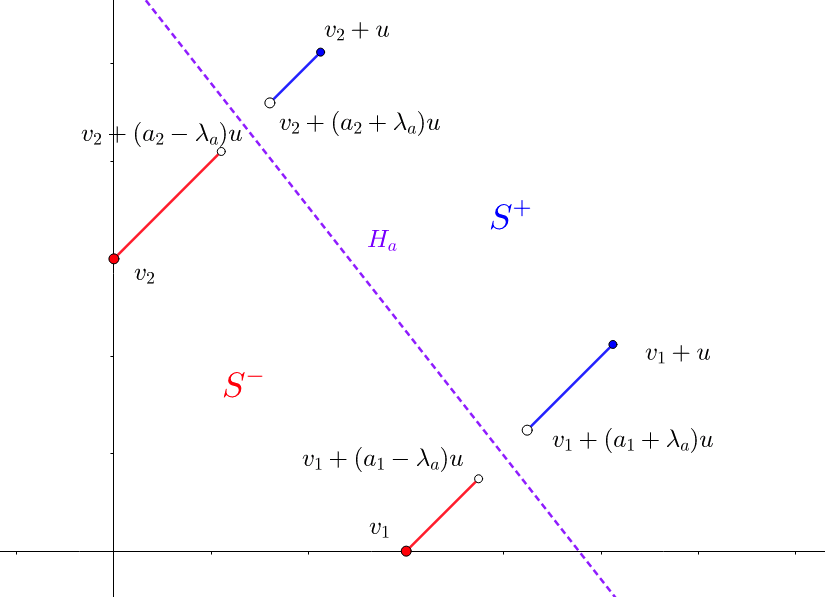
\includegraphics[scale=0.5]{d_a_pic}
\vspace{.3in}
\caption{An illustration of $\D_a$ in two dimensions. $S^-$ is shown in red, and $S^+$ is shown in blue. The decision boundary, $H_a$, of the optimal linear classifier, $f_{w^a, 1}$, is shown in purple. }
\label{fig:d_a_illustration}
\end{figure}

We include an example of such a distribution in Figure \ref{fig:d_a_illustration}. Next, we explicitly compute a linear classifier that linearly $r$-separates $\D_a$.

\begin{defn}\label{def:normal_vector}
Let $a \in [0,1]^d$, and let $\overline{a} = \sum_{i=1}^d a_i.$ Then let $w^a$ be defined as $$w_i^a = \frac{1}{\rr} - \frac{da_i}{\rr\sqrt{d} + d\rr\overline{a}}.$$ 
\end{defn}

\begin{lem}\label{lem:normal_vector_works}
$w^a$ satisfies $\langle w^a, u\rangle = \frac{d}{\sqrt{d} + d\overline{a}}$ and $\langle w^a, v_i + a_iu \rangle = 1,$ for all $1 \leq i \leq d.$ 
\end{lem}

\begin{proof}
By the definitions of $v_i, u$, we have that 
\begin{equation*}
\begin{split}
\langle w^a, u \rangle &= \langle w^a, \frac{1}{\sqrt{d}}\sum_1^d v_i \rangle \\
&= \frac{1}{\sqrt{d}} \sum_1^d Rw_i^a \\
&= \frac{1}{\sqrt{d}} \sum_1^d 1 - \frac{da_i}{\sqrt{d} + d\overline{a}} \\
&= \frac{1}{\sqrt{d}} \sum_1^d \frac{\sqrt{d} + d\overline{a} - da_i}{\sqrt{d} + d\overline{a}} \\
&= \frac{1}{\sqrt{d}} \frac{d\sqrt{d}}{\sqrt{d} + d\overline{a}} = \frac{d}{\sqrt{d} + d\overline{a}},
\end{split}
\end{equation*}
Which proves the first claim. Next, we also have that $\langle w^a, v_i \rangle = Rw_i^a$. Summing these, we get $$Rw_i^a + \frac{da_i}{\sqrt{d} + d\overline{a}} = 1 - \frac{da_i}{\sqrt{d} + d\overline{a}} + \frac{da_i}{\sqrt{d} + d\overline{a}} = 1,$$ as desired. 
\end{proof}

We now prove that $\D_a$ is linearly $r$-separated.

\begin{lem}\label{lem:separation}
$\D_a$ is linearly $r$-separated by the classifier $f_{w_a, 1}$.
\end{lem}

\begin{proof}
Let $H_a$ denote the hyperplane passing through $\{v_i + a_iu: 1 \leq i \leq d\}$. By Lemma \ref{lem:normal_vector_works}, $H_a$ is the decision boundary of $f_{w_a, 1}$.  Referring to Figure \ref{fig:d_a_illustration}, we see that $\cup S^+$ lies entirely above $H_a$ while the set $\cup S^-$ lies entirely below the hyperplane $H_a$, which the classifier $f_{w^a, 1}$ has accuracy $1$ with respect to $\D_a$. It suffices to show that $f_{w^a, 1}$ is robust everywhere. In order to do this, we must show that all points in the support of $\D_a$ have $\ell_p$ distance at least $r$ from $H_a$. 

Fix any $1 \leq i \leq d$. Since the $\ell_p$ distance metric is invariant under translation and scales linearly with dilations, it follows that the point $x_i = v_i + (a_i - \lambda_a)u$ is the closest point on the segment $[v_i, v_i+(a_i - \lambda_a)u)$ to $H_a$. Suppose $x_i$ has distance $D$ under the $\ell_p$ norm to $H_a$. Then the key observation is that the $\ell_p$ ball, $B_p(x_i, D)$, must be tangent to $H_a$. Expressing this as an equation, we have $\max_{z \in B_p(x_i, D)} \langle z, w^a \rangle = 1,$ which can be re-written as $$\max_{||z - x_i||_p \leq D} \langle z - x_i, w^a \rangle = 1 - \langle x_i, w^a \rangle.$$ By Lemma \ref{lem:normal_vector_works} , $\langle w^a, u \rangle = \frac{d}{\sqrt{d} + d\overline{a}}$ and $\langle w^a, v_i + a_iu \rangle = 1$. Substituting this, we see that 
\begin{equation*}
\begin{split}
1 - \langle x_i, w^a \rangle &= 1 - \langle v_i + a_iu - \lambda_a u, w^a \rangle \\
&= 1 - \langle v_i + a_iu, w^a \rangle + \langle \lambda_a u, w^a \rangle \\
&= \langle \lambda_a u, w^a \rangle \\
&= \frac{d\lambda_a}{\sqrt{d} + d\overline{a}}.
\end{split}
\end{equation*}

However, by using the dual norm, we see that $\max_{||z - x_i||_p \leq D} \langle z - x_i, w^a \rangle = D||w^a||_q$. Thus it follows that
\begin{equation*}
\begin{split}
D &= \frac{d\lambda_a}{(\sqrt{d} + d\overline{a})||w^a||_q} \\
&= \frac{d\frac{r}{\rr}f_q(a)}{(\sqrt{d} + d\overline{a})||w^a||_q} \\
&= \frac{d\frac{r}{\rr}\sqrt[q]{\sum_1^d |\frac{1}{\sqrt{d}} + \overline{a} - a_i|^q}}{(\sqrt{d} + d\overline{a})||w^a||_q} \\
&= \frac{r\sqrt[q]{\sum_1^d |\frac{1}{\rr}\frac{\sqrt{d} + d\overline{a} - da_i}{(\sqrt{d} + d\overline{a})}|^q}}{||w^a||_q} \\
&= \frac{r||w^a||_q}{||w^a||_q} = r.
\end{split}
\end{equation*}
We can use an analogous argument holds for $v_i + (a_i + r_a)u$, the closest point to $H_a$ in $S^+$. Thus each point in the support of $D^a$ has distance strictly larger than $r$ (as the endpoints were not included) to $H_a$. Consequently $f_{w^a, 1}$ linearly $r$-separates $D^a$, as desired. 
\end{proof}

\subsubsection{Defining $\dd$}\label{subsubsec:dd}

Now that we have defined $\D_a$, we turn our attention to defining $\A$, which requires us to specify a distribution over valid choices of $a$. In particular, although $\D_a$ is defined for $a \in [0, 1]^d$, we will require a more stringent condition on $a$ for our construction to work. To this end, we begin by defining $\Delta$, a key parameter that characterizes the domain of $a$. To define $\dd$, we use the following lemma.

\begin{lem}\label{lem:dd}
There exists a real number $\dd > 0$ such that for all $l \in \{2, q\}$, and for all $a \in [\frac{1}{2} - \dd, \frac{1}{2} + \dd]^d$, $$||\nabla f_l(a)||_2 \leq \frac{1}{d^2\sqrt{d}},$$ where $f_l$ is as defined in Definition \ref{defn:function_f}.
\end{lem}

\begin{proof}
Since $1 \leq q < \infty$, we see that for both choices of $l$, the function $h_l(x) = (\frac{1}{\sqrt{d}} - x)^l$ is a convex function for $x \in [-\frac{1}{2\sqrt{d}}, \frac{1}{2\sqrt{d}}]$. Thus, if $\sum_1^d x_i = 0$, then by Jensen's inequality, $\sum_1^d h_l(x_i) \geq \sum_1^d h_l(0)$. Applying this, we see that for all $l \in \{2, q\}$ and for all $a \in [\frac{1}{2} - \frac{1}{4\sqrt{d}}, \frac{1}{2} + \frac{1}{4\sqrt{d}}]^d$, 
\begin{equation*}
\begin{split}
f_l(a) &= \sqrt[l]{\sum_1^d |\frac{1}{\sqrt{d}} + \overline{a} - a_i|^l} \\
&= \sqrt[l]{\sum_1^d \left(\frac{1}{\sqrt{d}} + \overline{a} - a_i\right)^l} \\
&= \sqrt[l]{\sum_1^d h_l(a_i - \overline{a})} \\
&\geq \sqrt[l]{\sum_1^d h_l(0)} \\
&= f_l((\frac{1}{2}, \frac{1}{2}, \dots, \frac{1}{2})),
\end{split}
\end{equation*}
with the first equality holding since $\overline{a} - a_i < \frac{1}{\sqrt{d}}$ and the first inequality holding since $\sum_1^d a_i - \overline{a} = 0$. Thus $f_l(a)$ must be locally minimized when $a = (\frac{1}{2}, \frac{1}{2}, \dots, \frac{1}{2})$, and it follows that $$||\nabla f_l(\frac{1}{2}, \frac{1}{2}, \dots, \frac{1}{2})||_2 = 0, \text{ for } l = 2, q.$$ Now observe that the map $H(a) = \max_{l \in \{2, q\}} ||\nabla f_l(a)||_2$ is a continuous map as long as $|a_i - \overline{a}| < \frac{1}{\sqrt{d}}$ for all $1 \leq i \leq d$. Thus there exists an open neighborhood $U$ about $(\frac{1}{2}, \frac{1}{2}, \dots, \frac{1}{2})$ such that $H(a) \leq \frac{1}{d^2\sqrt{d}}$ for all $a \in U$. Taking $\dd$ so that $[\frac{1}{2} - \dd, \frac{1}{2} + \dd]^d \subseteq U$ suffices. 
\end{proof}

\begin{defn}\label{defn:Delta}
Let $\Delta$ be any constant for which Lemma \ref{lem:dd} holds. In particular, $\Delta$ only depends on $\ell_p$, the robustness norm, and $d$, the dimension.
\end{defn}

\subsubsection{Defining $\g_1$ and $\g_2$}\label{subsubsec:g1g2}

In this section, we define functions $\g_1, \g_2: [0, \frac{\Delta}{3}] \to [0, \frac{\Delta}{3}]$ which we will use to specify $\A$. Before defining $\g_1$ and $\g_2$, we will first prove several technical lemmas.

\begin{lem}\label{lem:phi_s}
Let $I \subseteq \R$ be an interval, and $\Phi:I \to \R$ be a strictly convex function.  For any $s \in \R$ and $t \geq 0$, let $\Phi_s(t) = \Phi(s-t) + \Phi(s + t)$. Then $\Phi_s$ is a strictly increasing function.
\end{lem}

\begin{proof}
Fix $s$, and let $0 \leq t_1 < t_2$. Then we see that by Jensen's inequality (for strictly convex functions), $$\Phi(s + t_1) < \frac{(t_2-t_1)\Phi(s+t_2)}{t_1 + t_2} + \frac{2t_1\Phi(s-t_1)}{t_1 + t_2},$$ and $$\Phi(s - t_1) < \frac{(t_2-t_1)\Phi(s-t_2)}{t_1 + t_2} + \frac{2t_1\Phi(s+t_1)}{t_1 + t_2}.$$ Summing these inequalities, we see that 
\begin{equation*}
\begin{split}
\Phi_s(t_1) &= \Phi(s - t_1) + \Phi(s + t_1) \\
&< \frac{(t_2-t_1)\Phi(s+t_2)}{t_1 + t_2} + \frac{2t_1\Phi(s-t_1)}{t_1 + t_2} + \frac{(t_2-t_1)\Phi(s-t_2)}{t_1 + t_2} + \frac{2t_1\Phi(s+t_1)}{t_1 + t_2} \\
&= \frac{t_2 - t_1}{t_1 + t_2}(\Phi(s +t_2) + \Phi(s - t_2)) + \frac{2t_1}{t_1 + t_2}(\Phi(s - t_1) + \Phi(s + t_1)) \\
&= \frac{t_2 - t_1}{t_1 + t_2}\Phi_s(t_2) + \frac{2t_1}{t_1 + t_2}\Phi_s(t_1).
\end{split}
\end{equation*}
Rearranging this yields $\Phi_s(t_1) < \Phi_s(t_2)$, as desired.
\end{proof}

\begin{lem}\label{lem:lipschitz}
Let $I \subseteq \R$ be an interval, $\Phi:I \to \R$ be a strictly convex continuous function, and  $x, y, z \in I$ be real numbers with $x < y < z$. Let $\epsilon >0$ be such that $x - \epsilon \in I$ and $y + \epsilon \leq z - \epsilon$. Then there exist unique $\delta, \gamma >0$ such that the following hold: $$\delta + \gamma = \epsilon,$$ $$\Phi(x-\delta) + \Phi(y + \epsilon) + \Phi(z - \gamma) = \Phi(x) + \Phi(y) + \Phi(z)$$
\end{lem}

\begin{proof}
Fix any $\epsilon$ satisfying the desired conditions, and define $\Theta: [0, \epsilon] \to \R$ as $\Theta(t) = \Phi(x - t) + \Phi(y + \epsilon) + \Phi(z + t - \epsilon)$. Then, utilizing the definition of $\Phi_s$ from Lemma \ref{lem:phi_s}, we see that $$\Theta(t) = \Phi_{\frac{x + z - \epsilon}{2}}(\frac{z - x - \epsilon}{2} + t) + \Phi(y + \epsilon).$$ By Lemma \ref{lem:phi_s}, it follows that $\Theta$ is strictly increasing in $t$, and since $\Phi$ is continuous, so is $\Theta$. Next, we bound $\Theta(0)$ and $\Theta(\epsilon)$ to put us in the configuration to apply the intermediate value theorem. To bound $\Theta(0)$, we have
\begin{equation*}
\begin{split}
\Theta(0) &= \Phi(x) + \Phi(y + \epsilon) + \Phi(z - \epsilon) \\
&= \Phi(x) + \Phi_{\frac{y+z}{2}}(\frac{z - y}{2} - \epsilon) \\
&< \Phi(x) + \Phi_{\frac{y+z}{2}}(\frac{z - y}{2}) \\
&= \Phi(x) + \Phi(y) + \Phi(z),
\end{split}
\end{equation*}
and to bound $\Theta(\epsilon)$, we have 
\begin{equation*}
\begin{split}
\Theta(\epsilon) &= \Phi(x - \epsilon) + \Phi(y + \epsilon) + \Phi(z) \\
&= \Phi_{\frac{x+y}{2}}(\frac{y- x}{2} + \epsilon) + \Phi(z)\\
&> \Phi_{\frac{x+y}{2}}(\frac{y - x}{2}) + \Phi(z) \\
&= \Phi(x) + \Phi(y) + \Phi(z).
\end{split}
\end{equation*}
Together, these equations imply $\Theta(0) < \Phi(x) + \Phi(y) + \Phi(z) < \Theta(\epsilon)$. Since $\Theta$ is strictly increasing and continuous, there exists a unique $\delta \in [0, \epsilon]$ such that $\Theta(\delta) = \Phi(x) + \Phi(y) + \Phi(z)$. Setting $\gamma = \epsilon - \delta$, we see that $$\Theta(\delta) = \Phi(x - \delta) + \Phi(y + \epsilon) + \Phi(z - \gamma) = \Phi(x) + \Phi(y) + \Phi(z),$$ as desired.


\end{proof}



Next, we define a function that will be useful for simplifying notation, both in this section and subsequent ones.

\begin{defn}\label{defn:F_the_function}
Let $\Delta$ be as in definition \ref{defn:Delta}. For $x, y, z \in [0, \frac{\dd}{3}]$, let $$F(x, y, z) = \sqrt[q]{\left(\frac{1}{\sqrt{d}} - x\right)^q + \left(\frac{1}{\sqrt{d}} - \frac{2\Delta}{3} + y\right)^q + \left(\frac{1}{\sqrt{d}} + \frac{2\Delta}{3} + z\right)^q}.$$
\end{defn}

We now define $\g_1, \g_2$.
\begin{cor}\label{cor:lipschitz_maps}
Let $\Delta$ be as in definition \ref{defn:Delta}. There exist $1$-Lipshitz, monotonically non-decreasing functions $\g_1, \g_2: [0, \frac{\dd}{3}] \to [0, \frac{\dd}{3}]$ such that for all $t \in [0, \frac{\dd}{3}]$, $\g_1(t) + \g_2(t) = t$ and $F(t, \g_1(t), \g_2(t)) = F(0, 0, 0)$. 
\end{cor}
\begin{proof}
We have two cases.
\paragraph{Case 1: $1 < q < \infty$:} Let $\Phi: [-\Delta, \Delta] \to \R$ be defined as $\Phi(x) = (\frac{1}{\sqrt{d}} - x)^q$. Since $q > 1$, and $\Delta < \frac{1}{\sqrt{d}}$, $\Phi$ is strictly convex. Observe that $$F(x, y, z)^q = \Phi(x) + \Phi(2\frac{\dd}{3} - y) + \Phi(-2\frac{\dd}{3} - z).$$ Next, fix any $t \in [0, \frac{\Delta}{3}]$. Then observe that $-\frac{2\Delta}{3} \geq -\Delta$ and that $\frac{2\Delta}{3} - t \geq 0 + t$. This puts us in the configuration to apply Lemma \ref{lem:lipschitz}. In particular, there exist unique reals $\delta_t, \gamma_t > 0$ such that $$\delta_t + \gamma_t = t,$$ $$\Phi(-\frac{2\Delta}{3} - \delta_t) + \Phi(t) + \Phi(\frac{2\Delta}{3} - \gamma_t) = \Phi(-\frac{2\Delta}{3}) + \Phi(0) + \Phi(\frac{2\Delta}{3}).$$ We now define $g_1, g_2: [0, \frac{\Delta}{3}] \to [0, \frac{\Delta}{3}]$ as $$g_1(t) = \gamma_t\text{ and }g_2(t) = \delta_t.$$ Then it is clear that $F(0,0,0) = F(t, g_1(t), g_2(t))$ and $g_1(t) + g_2(t)$ (by directly substituting into the equations above). All that remains is to show that $g_1$ and $g_2$ are 1-Lipschitz. 

Fix any $0 \leq t_1 < t_2 \leq \frac{\Delta}{3}$, and let $t_2 - t_1 = \epsilon$. The key idea is to apply Lemma \ref{lem:lipschitz} to $-\frac{2\Delta}{3} - g_2(t_1)<  t_1 < \frac{2\Delta}{3} - g_1(t_1)$ and $\epsilon$. To do so, we first check the conditions of the lemma. 

We have that $$-\frac{2\Delta}{3} - g_2(t_1) - \epsilon \geq -\frac{2\Delta}{3} - t_1 - \epsilon = -\frac{2\Delta}{3} - t_2 \geq -\Delta,$$ and 
\begin{equation*}
\begin{split}
t_1 + \epsilon &= t_2 \\
&\leq \frac{\Delta}{3} \\
&\leq \frac{2\Delta}{3} - t_2 \\
&= \frac{2\Delta}{3} - t_1 - \epsilon \\
&\leq \frac{2\Delta}{3} - g_1(t_1) - \epsilon.
\end{split}
\end{equation*}

Thus $\epsilon$ satisfies the necessary conditions for Lemma \ref{lem:lipschitz}. Since $\Phi$ is strictly convex, by Lemma \ref{lem:lipschitz}, there exist unique $\delta, \gamma > 0$ with $\delta+ \gamma = \epsilon$ such that $$\Phi(-\frac{2\Delta}{3} - g_2(t_1) - \delta) + \Phi(t_1 + \epsilon) + \Phi(\frac{2\Delta}{3} - g_1(t_1) - \gamma) = \Phi(-\frac{2\Delta}{3} - g_2(t_1)) + \Phi(t_1) + \Phi(\frac{2\Delta}{3} - g_1(t_1)).$$ However, by the definition of $g_1, g_2$, we see that both of these quantities are equal to $F(0,0,0)^q$. Moreover, again by the definition of $g_1, g_2$, we also have that $g_1(t_2)$ and $g_2(t_2)$ are the unique real numbers in $[0, \frac{\Delta}{3}$ that satisfy $$\Phi(-\frac{2\Delta}{3} - g_2(t_2)) + \Phi(t_2) + \Phi(\frac{2\Delta}{3}+g_1(t_2)) = F(0,0,0)^q.$$ Thus, it follows that $g_2(t_2) = g_2(t_1) + \delta$ and $g_1(t_2) = g_1(t_1) + \gamma$. However, $t_2 - t_1 = \epsilon$, and $\delta, \gamma < \epsilon$ (since they sum to $\epsilon$). Thus, we see that $|g_1(t_2) - g_1(t_1)| \leq |t_2 - t_1|$ and $|g_2(t_2) - g_2(t_1)| \leq |t_2 - t_1|$. Since $t_1$ and $t_2$ were arbitrary, it follows that $g_1$ and $g_2$ are both $1$-Lipschitz, as desired. 

Finally, since $\delta, \gamma > 0$, it follows that $g_2(t_2) > g_2(t_1)$ and $g_1(t_2) > g_1(t_1)$. Since $t_1, t_2$ were arbitrary, it follows that $g_1, g_2$ are monotonically non-decreasing.

\paragraph{Case 2: $q = 1$} In this case, since $\Delta < \frac{1}{\sqrt{d}}$ (Lemma \ref{lem:dd}), we see that $F(x, y, z) = \frac{3}{\sqrt{d}} + y + z - x$. Setting $\g_1(t) = \g_2(t) = \frac{t}{2}$ suffices, and clearly satisfies the desired properties. 
\end{proof}

\begin{defn}\label{defn:g_1_and_g_2}
Let $\Delta$ be as defined in Definition \ref{defn:Delta}. We let $g_1, g_2: [0, \frac{\Delta}{3}] \to [0, \frac{\Delta}{3}]$ be defined as any function satisfying the conditions of Corollary \ref{cor:lipschitz_maps}.
\end{defn}

\subsubsection{Putting it all together: defining $\A$}\label{subsubsec:finalA}

We are now ready to define $\A$. For convenience, we assume $d$ is a multiple of $3$.
\begin{defn}\label{defn:A}
Let $\Delta, g_1$, and $g_2$ be as defined in Definitions \ref{defn:Delta} and \ref{defn:g_1_and_g_2}. Then $\A$ is defined as the distribution of distributions $\D_a$ where $a$ is a random vector constructed as follows. Let $t_1, t_2, \dots t_{d/3}$ be drawn i.i.d from the uniform distribution over $[0, \frac{\dd}{3}]$. Then for $1 \leq i \leq d/3$, we let
	\begin{itemize}
		\item $a_i = \frac{1}{2} + t_i$.
		\item $a_{i+d/3} = \frac{1}{2} + 2\frac{\dd}{3} - g_1(t_i)$.
		\item $a_{i + 2d/3} = \frac{1}{2} - 2\frac{\dd}{3} - g_2(t_i).$
	\end{itemize}
Together the variables $a_1, a_2, \dots, a_d$ compose $a$. Thus a random distribution $\D \sim \A$ can be constructed by sampling $a$ as above and setting $\D = \D_a$.
\end{defn}

We now show that for all $\D_a \sim \A$, $\lambda_a$ (Definition \ref{def:w_dist}) is constant.

\begin{lem}\label{lem:cons_lambda}
There exists a constant $\Lambda$ such that for all $\D_a \sim \A$, $\lambda_a = \Lambda$. 
\end{lem}

\begin{proof}
Let $\D_a \sim \A$ be arbitrary. By Lemma \ref{cor:lipschitz_maps}, for all $1 \leq i \leq d$, $g_1(t_i) + g_2(t_i) = t_i$. Substituting this, we see that 
\begin{equation*}
\begin{split}
\overline{a} &= \frac{1}{d}\sum_1^d a_i \\
&= \frac{1}{d}\sum_1^{d/3} (\frac{1}{2} + t_i) + (\frac{1}{2} + \frac{2\Delta}{3} - g_1(t_i)) + (\frac{1}{2} - \frac{2\Delta}{3} - g_2(t_i)) \\
&= \frac{1}{d}\sum_1^{d/3} \frac{3}{2} \\
&= \frac{1}{2}.
\end{split}
\end{equation*}

Recall that $\lambda_a = \frac{r}{R}f_q(a) = \frac{r}{R}\sqrt[q]{\sum_1^d |\frac{1}{\sqrt{d}} + \overline{a} - a_i|^q}$. By substituting that $\overline{a} = \frac{1}{2}$ and expressing each $a_i$ in terms of $t_i$, we see that 
\begin{equation*}
\begin{split}
\lambda_a &=  \frac{r}{R}\sqrt[q]{\sum_1^d |\frac{1}{\sqrt{d}} + \overline{a} - a_i|^q}\\
&= \frac{r}{R}\sqrt[q]{\sum_{i=1}^{d/3} \left|\frac{1}{\sqrt{d}} + \frac{1}{2} - (\frac{1}{2} + t_i)\right|^q + \left|\frac{1}{\sqrt{d}} + \frac{1}{2} - \left(\frac{1}{2} + \frac{2\Delta}{3} - g_1(t_i)\right)\right|^q +  \left|\frac{1}{\sqrt{d}} + \frac{1}{2} - \left(\frac{1}{2} - \frac{2\Delta}{3} - g_2(t_i)\right)\right|^q} \\
 &= \frac{r}{R}\sqrt[q]{\sum_1^{d/3} \left|\frac{1}{\sqrt{d}} - t_i\right|^q + \left|\frac{1}{\sqrt{d}} + g_1(t_i) - \frac{2\Delta}{3}\right|^q + \left|\frac{1}{\sqrt{d}} + g_2(t_i) + \frac{2\Delta}{3}\right|^q} \\
&= \frac{r}{R}\sqrt[q]{\sum_1^{d/3}F(t_i, g_1(t_i), g_2(t_i))^q}, \\
\end{split}
\end{equation*}
where $F$ is defined as in Definition \ref{defn:F_the_function}. Next, by Corollary \ref{cor:lipschitz_maps}, $F(t_i, g_1(t_i), g_2(t_i)) = F(0,0,0)$ for all $1 \leq i \leq \frac{d}{3}$. Thus, if we set $\Lambda = \frac{r}{R}(\frac{d}{3})^{1/q}F(0,0,0)$, we have 
\begin{equation*}
\begin{split}
\lambda_a &= \frac{r}{R}\sqrt[q]{\sum_1^{d/3} F(t_i, g_1(t_i), g_2(t_i))^q} \\
&= \frac{r}{R}\sqrt[q]{\sum_1^{d/3}F(0,0,0)^q} \\
&= \frac{r}{R}\sqrt[q]{\frac{d}{3}F(0,0,0)^q} \\
&=  \frac{r}{R}(\frac{d}{3})^{1/q}F(0,0,0) = \Lambda,
\end{split}
\end{equation*}
proving the claim.
\end{proof}

\begin{defn}\label{defn:big_lambda}
We define $\Lambda = \frac{r}{R}(\frac{d}{3})^{1/q}F(0,0,0)$, where $F$ is defined as in Definition \ref{defn:F_the_function}.
\end{defn}

Next, we compute upper and lower bounds on $\Lambda$, both of which will be useful for subsequent lemmas. 
\begin{lem}\label{lem:lambda_bounds}
$\frac{1}{9} < \Lambda < \frac{1}{3}$. 
\end{lem}

\begin{proof}
By definition, $\Lambda = \frac{d}{3}^{1/q}F(0, 0, 0)$. Substituting the definition of $f$, we see that  $F(0, 0, 0) = \sqrt[q]{|\frac{1}{\sqrt{d}}|^q + |\frac{1}{\sqrt{d}} - \frac{2\Delta}{3}|^q + |\frac{1}{\sqrt{d}} + \frac{2\Delta}{3}|^q},$ and consequently, $$3^{1/q}|\frac{1}{\sqrt{d}} - \frac{2\Delta}{3}| \leq F(0, 0, 0) \leq 3^{1/q}|\frac{1}{\sqrt{d}} + \frac{2\Delta}{3}|.$$ By definition, $\frac{2\Delta}{3} < \frac{1}{2\sqrt{d}}$. It follows that $$\frac{r}{R}\frac{d^{1/q}}{2\sqrt{d}} < \Lambda < \frac{r}{R}\frac{3d^{1/q}}{2\sqrt{d}}.$$ Finally, since $\frac{r}{R} = \frac{2\sqrt{d}}{9d^{1/q}}$, substituting this yields $\frac{1}{9} < \Lambda < \frac{1}{3}$, as desired.
\end{proof}

Next, we show that for all $\D_a \in \A$, the aspect ratio (Definition \ref{defn:aspect_ratio}), $\rho(\D_a)$, is bounded by a constant.

\begin{lem}\label{lem:large_margin}
For all $\D_a \in \A$, we have $\rho(\D_a) \leq 18\sqrt{3}$. 
\end{lem}

\begin{proof}
We first bound the $\ell_2$ margin, $\gamma(\D_a)$ (Definition \ref{defn:margin}). Recall that the margin, $\gamma(\D_a)$ is described as the largest possible $\ell_2$ distance from the support of $\D_a$ to the decision boundary of a linear classifier. Thus, we can lower bound $\gamma(\D_a)$ by computing the distance from the support of $\D_a$ to $H_a$, the decision boundary of $f_{w^a, 1}$ (Definition \ref{def:normal_vector}).

By referring to Figure \ref{fig:d_a_illustration} (in Section \ref{subsubsec:D_a}), it becomes clear that the closest point (under the $\ell_2$ margin) from $S^-$ to $H_a$ is the point $v_i + (a_i - \lambda_a)u$, for some value of $i$. Thus it suffices to compute the $\ell_2$ distance from this point to the plane $H_a$. 

Recall that by Lemma \ref{lem:normal_vector_works}, the point $v_i + a_iu$ satisfies $\langle w^a, v_i + a_iu \rangle = 1$, and consequently must lie on the hyperplane $H_a$. Let $D$ denote the $\ell_2$ distance from $v_i + (a_i - \lambda_a)u$ to $H_a$. Since $w^a$ is the normal vector to $H_a$, it follows that
\begin{equation*}
\begin{split}
D &= \langle v_i + a_iu - (v_i + (a_i - \lambda_a)u), \frac{w^a}{||w^a||_2} \rangle \\
&= \frac{\langle \lambda_a u, w^a \rangle}{||w^a||_2} \\
&\numeq{1} \frac{\langle \Lambda u, w^a \rangle}{||w^a||_2} \\
&\numeq{2} \frac{\Lambda \frac{d}{\sqrt{d} + d\overline{a}}}{||w^a||_2}  \\
&\numeq{3} \frac{\Lambda \frac{d}{\sqrt{d} + d\overline{a}}}{\sqrt{\sum_1^d \left(\frac{\sqrt{d} + d\overline{a} - da_i}{R(\sqrt{d} + d\overline{a}}\right)^2}} \\
&= \frac{R\Lambda}{\sqrt{\sum_1^d (\frac{1}{\sqrt{d}} + \overline{a} - a_i)^2}} \\
&\numeq{4} \frac{R\Lambda}{f_2(a)}.
\end{split}
\end{equation*}
Here, (1) holds by Lemma \ref{lem:cons_lambda}, (2) holds by Lemma \ref{lem:normal_vector_works}, (3) holds by Definition \ref{def:normal_vector}, and (4) holds by Definition \ref{defn:function_f}.

Next, observe that since $\D_a \sim \A$, we must have $a \in [\frac{1}{2} - \Delta, \frac{1}{2} + \Delta]^d$. Thus it follows that $||a - (\frac{1}{2}, \frac{1}{2}, \dots, \frac{1}{2})||_2 \leq \Delta\sqrt{d}$. However, by applying Lemma \ref{lem:dd}, we also see that $f_2$ is $\frac{1}{d^2\sqrt{d}}$-Lipschitz over $[\frac{1}{2} - \Delta, \frac{1}{2} + \Delta]^d$. Thus, it follows that $$f_2(a) \leq f_2(\frac{1}{2}, \frac{1}{2}, \dots, \frac{1}{2}) + \Delta\sqrt{d} \frac{1}{d^2\sqrt{d}} \leq 2,$$ with the latter inequality holding from the definition of $\Delta$. 

Substituting this and applying Lemma \ref{lem:lambda_bounds}, we see that $$\gamma(\D_a) \geq \frac{R\Lambda}{2} \geq \frac{R}{18}.$$ Next, to bound the aspect ratio, $\rho(\D_a)$, we must also bound the $\ell_2$ diameter of $\D_a$. However, the $\ell_s$ diameter of $\D_a$ is $R\sqrt{3}$, since it is the distance from $v_i + u$ to $v_j$ for $i \neq j$. Thus, it follows that $$\rho(\D_a) = \frac{diam_2(\D_a)}{\gamma(\D_a)} \leq \frac{R\sqrt{3}}{R/18} = 18\sqrt{3},$$ as desired. 
\end{proof}

Note that a tighter analysis (and selection of $\Delta$) can give a smaller bound for $\rho(\D_a)$, but the most important fact is that $\rho(\D_a) = O(1)$. 

\subsection{Bounding the expected robust loss}\label{subsec:bound_expectation}

In this section, we finally prove our lower bound, Theorem \ref{thm:lower}. This will require a few important steps, which we have separated into the following subsections. 
\begin{itemize}
	\item In section \ref{subsubsec:loss_bounding}, we give a useful lower bound for the loss $\L_r(f, \D_a)$ where $f$ is an arbitrary linear classifier. 
	\item In section \ref{subsubsec:posterior}, we give an explicit computation for the posterior distribution $\A|S$ where $S \sim \D_a^n$ is the observed training sample. 
	\item Finally, in section \ref{subsubsec:proof}, we present the proof of Theorem \ref{thm:lower}.
\end{itemize}

\subsubsection{Bounding the loss $\L_r(f, \D_a)$}\label{subsubsec:loss_bounding}

In this section, we find a lower bound on the loss $\L_r(f, \D_a)$ where $f$ is a linear classifier. We begin by first restricting $f$ to be in the set of classifiers $$f \in \{f_{w^b, 1}: b \in [0, 1]^d\},$$ where $w^b$ is as defined in Definition \ref{def:normal_vector}. These are precisely the classifiers that have a decision boundary that passes through some point on every line segment in $\{[v_i, v_i + u]: 1 \leq i \leq d\}$. We are able to only consider these classifiers since all other linear classifiers clearly have a very high loss with respect to $\D_a$ as they necessarily misclassify at least half the points on the line segment $[v_i, v_i + u]$ for some value of $i$. 

We now find an initial lower bound on $\L_r(f_{w^b, 1}, \D_a)$.

\begin{lem}\label{lem:loss_bound_general}
Fix any $\D_a \in \A$, and let $b \in [0,1]^d$ be arbitrary. Let $w^b$ be the vector defined as in Definition \ref{def:normal_vector}, and $\lambda_b = \frac{r}{\rr}\f_q(b)$ where $f$ is as defined in Definition \ref{defn:function_f}. Then $$\L_r(f_{w^b, 1}, \D_a) \geq \frac{d(\lambda_b - \lambda_a) + \sum_1^d|a_i - b_i|}{d - 2d\Lambda}.$$ 
\end{lem}

\begin{proof}
By Lemma \ref{lem:separation}, $f_{w^b, 1}$ precisely $r$-separates $\D_b$. This implies that for all $1 \leq i \leq d$,
$$f_{w^b, 1}(x) = \begin{cases} 1 & x \in (v_i + (b_i + \lambda_b)u, v_i + u] \\-1 & x \in [v_i, v_i + (b_i - \lambda_b)u) \\ \text{not robust} & x \in [v_i + (b_i - \lambda_b)u, v_i + (b_i + \lambda_b)u] \end{cases}.$$ Without loss of generality, suppose that $b_i \geq a_i$. The key observation is that for all $1 \leq i \leq d$, if $x \in [v_i + (a_i + \lambda_a)u, v_i + (b_i + \lambda_b)u]$, then $f_{w^b, 1}(x) = -1$ for $f_{w^b, 1}$ is not robust at $x$. In both cases, we see that $f_{w^b, 1}$ is either inaccurate or not robust for all points in $[v_i + (a_i + \lambda_a)u, v_i + (b_i + \lambda_b)u]$. 

This interval has $\ell_2$ length at least $(|a_i - b_i| + (\lambda_b - \lambda_a))||u||_2$. Note that in the case that $a_i \leq b_i$ we can get an identical expression. Thus,  combining this for all $i$, we see that $f_{w^b, 1}$ is either inaccurate or not robust for a total length of $[d(\lambda_b - \lambda_a) + \sum_1^d |a_i - b_i|]||u||_2$. Dividing by the total length of the support of $\D_a$, we find that
\begin{equation*}
\begin{split}
\L_r(f_{w^b, 1}, \D_a) &\geq \frac{[d(\lambda_b - \lambda_a) + \sum_1^d |a_i - b_i|]||u||_2}{\sum_1^d ||[v_i, v_i + (a_i - \lambda_a)u) + (v_i + (a_i + \lambda_a)u, v_i + u]||_2} \\
&= \frac{[d(\lambda_b - \lambda_a) + \sum_1^d |a_i - b_i|]||u||_2}{\sum_1^d ||u_2||(1 - 2\lambda_a)} \\
&= \frac{d(\lambda_b - \lambda_a) + \sum_1^d |a_i - b_i|}{d(1 - 2\lambda_a)} \\
&= \frac{d(\lambda_b - \lambda_a) + \sum_1^d |a_i - b_i|}{d - 2d\Lambda},
\end{split}
\end{equation*}
with the last equality holding since by Lemma \ref{lem:cons_lambda}, $\lambda_a = \Lambda$. 
\end{proof}

\begin{lem}\label{lem:loss_bound_clever}
For all $\D_a \in \A$ and $b \in [0,1]^d$, $d(\lambda_a - \lambda_b) \leq \frac{1}{2}\sum_1^d |a_i - b_i|.$ 
\end{lem}

\begin{proof}
We have two cases.
\paragraph{Case 1:} $b \in [\frac{1}{2} - \Delta, \frac{1}{2} + \Delta]^d$.

Observe that $\lambda_b = \frac{r}{R}f_q(b)$ and $\lambda_a = \frac{r}{R}f_q(a)$. By Lemma \ref{lem:dd}, we see that $f_q$ is $\frac{1}{d^2\sqrt{d}}$-Lipschitz over the domain $[\frac{1}{2} - \Delta, \frac{1}{2} + \Delta]^d$. It follows that
\begin{equation*}
\begin{split}
\lambda_a - \lambda_b &= \frac{r}{R}(f_q(a) - f_q(b)) \\
&\leq \frac{r}{R}||a - b||_2\frac{1}{d^2\sqrt{d}} \\
&= \frac{2\sqrt{d}}{9d^{1/q}}||a - b||_2\frac{1}{d^2\sqrt{d}} \\
&< \frac{||a - b||_1}{2d},
\end{split}
\end{equation*}
with the last inequality following since the $\ell_2$ norm is smaller than the $\ell_1$ norm. Rearranging this gives the statement of the Lemma as desired.

\paragraph{Case 2: } $b \notin [\frac{1}{2} - \Delta, \frac{1}{2} + \Delta]^d$.

The main idea in this case will be to find $b' \in [\frac{1}{2} - \Delta, \frac{1}{2} + \Delta]^d$ such that $\lambda_b \geq \lambda_{b'}$ and such that $||b' - a||_1 \leq ||b - a||_1$. We will then apply Case 1 to get the desired result.

Without loss of generality, assume that $b_1 \geq b_2 \geq \dots \geq b_d$, and that $b_1, b_2, \dots b_k > \frac{1}{2} + \Delta$, $b_{k+1}, \dots, b_l \in [\frac{1}{2} - \Delta, \frac{1}{2} + \Delta]$, and $b_{l+1}, \dots b_d < \frac{1}{2} - \Delta$ for some values of $k$ and $l$. 

We will construct $b'$ in four steps. In each of these steps, we will change the values of $b_i$ such that neither $||a - b||_1$ nor $\lambda_b$ are increased. At each step, we let $b_i$ refer to its value at the end of the previous step. 


Finally, for reference, recall that $$\lambda_b = \frac{r}{R}f_q(b) = \frac{r}{R}\sqrt[q]{\sum_1^d |\frac{1}{\sqrt{d}} + \overline{b} - b_i|^q}.$$

\paragraph{Step 1:} We set $$b_i \leftarrow  \begin{cases} \frac{1}{k}\sum_{j=1}^k b_j & 1 \leq i \leq k \\b_i & k+1 \leq i \leq l \\  \frac{1}{d-l}\sum_{j=l+1}^d b_j& l+1 \leq i \leq d \end{cases}.$$ Since $a \in [\frac{1}{2} - \Delta, \frac{1}{2} + \Delta]^d$, we see that these operations do not change $||a - b||_1$, as $\sum_1^k |b_i - a_i| = \sum_1^k b_i - a_i$ and $\sum_{l+1}^d |b_i - a_i| = \sum_1^k a_i - b_i$. Also, observe that this operation preserves $\overline{b}$, and consequently since the function $f(x) = |\frac{1}{\sqrt{d}} + \overline{b} - x|^q$ is convex, we see that by Jensen's inequality that $\lambda_b$ is not increased by this operation.

\paragraph{Step 2:} Let $\beta = \sum_1^k(b_i - \frac{1}{2} - \Delta) - \sum_{l+1}^d (\frac{1}{2} - \Delta - b_i)$. Then we set $$b_i \leftarrow  \begin{cases} \begin{cases} \frac{1}{2} + \Delta + \frac{\beta}{k} & 1 \leq i \leq k \\ b_i & k+1 \leq i \leq l \\ \frac{1}{2} - \Delta & l+1 \leq i \leq d \end{cases} & \beta \geq 0 \\\begin{cases} \frac{1}{2} + \Delta & 1 \leq i \leq k \\ b_i & k+1 \leq i \leq l \\ \frac{1}{2} - \Delta + \frac{\beta}{d - l} & l+1 \leq i \leq d \end{cases} & \beta < 0\end{cases}.$$

Observe that this operation cannot increase $||a - b||_1$, since it doesn't increase $|a_i - b_i|$ for any value of $i$. Furthermore, this operation also does not change $\overline{b}$, and a similar convexity argument on the function $f(x) = |\frac{1}{\sqrt{d}} + \overline{b} - x|^q$ can show that this does not increase $\lambda_b$. 

Finally, if $\beta = 0$, we set $b' = b$, since we have reached a state such that $b \in [\frac{1}{2} - \Delta, \frac{1}{2} + \Delta]^d$. 

\paragraph{Step 3a:} We run this step if $\beta > 0$. Let $\alpha = \frac{\sum_{k+1}^d (\frac{1}{2} + \Delta - b_i)}{\beta}$. We then set  $$b_i \leftarrow  \begin{cases} \begin{cases} \frac{1}{2} + \Delta & 1 \leq i \leq k \\ (\frac{1}{2} + \Delta)(\frac{\alpha - 1}{\alpha}) + \frac{b_i}{\alpha} & k+1 \leq i \leq d \end{cases} & \alpha \geq 1 \\\begin{cases} \frac{1}{2} + \Delta + \frac{\beta}{k}(1 - \alpha) & 1 \leq i \leq k \\ \frac{1}{2} + \Delta & k+1 \leq i \leq d \end{cases} & \alpha < 1\end{cases}.$$ In this step, we can similarly verify that $||a - b||_1$ does not increase (as $|a_i - b_i|$ is strictly reduced for $1 \leq i \leq k$ by an exact amount to offset the possible increases in $|a_i - b_i|$ for $k+1 \leq i \leq d$). We also see by the same convexity argument as usual that this operation reduces $\lambda_b$. 

\paragraph{Step 3b:} We run this step if $\beta < 0$. Let $\alpha = \frac{\sum_{k+1}^d (b_i - \frac{1}{2} + \Delta)}{\beta}$. We then set  $$b_i \leftarrow  \begin{cases} \begin{cases} (\frac{1}{2} - \Delta)(\frac{\alpha - 1}{\alpha}) + \frac{b_i}{
\alpha} & 1 \leq i \leq l \\ \frac{1}{2} - \Delta & k+1 \leq i \leq d \end{cases} & \alpha \geq 1 \\\begin{cases} \frac{1}{2} - \Delta & 1 \leq i \leq l \\ \frac{1}{2} - \Delta + \frac{\beta}{d-l}(1-\alpha) & l+1 \leq i \leq d \end{cases} & \alpha < 1\end{cases}.$$ The justification for this step is analogous to 3a.

\paragraph{Step 4:} We only run this step if $\alpha < 1$. Observe that if $\alpha \geq 1$, then both Step 3a and Step 3b result with $b \in [\frac{1}{2} - \Delta, \frac{1}{2} + \Delta]^d$, which we set as $b'$. Observe that in this case, either $b_i \geq a_i$ for all $i$, or $b_i \leq a_i$ for all $i$. Thus we simply set $$b_i \leftarrow \overline{b}.$$ This operation does not change $||a - b||_1$, and it also reduces $\lambda_b$ (by a convexity argument). 

\paragraph{Step 5:} Finally, for all $1 \leq i \leq d\Delta$, we set $b_i = \frac{1}{2}-\Delta$ if $\overline{b} < \frac{1}{2} - \Delta$ and otherwise set $b_i = \frac{1}{2} - \Delta$ if $\overline{b} > \frac{1}{2} + \Delta$. In both cases, $\lambda_b$ is not changed, and $||a-b||_1$ is strictly reduced. In this step, we finally set $b' = b$. Note that we do not always reach this step, as it was possible in any of the previous steps to reach some $b \in [\frac{1}{2} - \Delta, \frac{1}{2} + \Delta]^d$, at which point we would have simply terminated.

\paragraph{Conclusion: } Through steps $1$ through $5$, we have found $b' \in [\frac{1}{2} - \Delta, \frac{1}{2} + \Delta]^d$ such that $\lambda_{b'} \leq \lambda_b$ and $||a - b'||_1 \leq ||a - b||_1$. By applying Case 1 to $b'$, we see that $d(\lambda_a - \lambda_{b'}) \leq \frac{1}{2}||a - b'||_1$. Thus, we have that $$\frac{1}{2}||a - b||_1 \geq \frac{1}{2}||a - b'||_1 \geq d(\lambda_a - \lambda_{b'}) \geq d(\lambda_a - \lambda_b),$$ which implies the result by the transitive property.


\end{proof}

From the previous two lemmas, we immediately have the following:
\begin{cor}\label{cor:l_1distancebound}
For all $\D_a \in \A$ and $b \in [0,1]^d$, $$\L_r(f_{w^b, 1}, \D_a) \geq \frac{1}{2d}\sum_1^d |a_i - b_i|.$$
\end{cor}

\begin{proof}
We have that
\begin{equation*}
\begin{split}
\L_r(f_{w^b, 1}, \D_a) &\numgeq{a} \frac{d(\lambda_b - \lambda_a) + \sum_1^d|a_i - b_i|}{d - 2d\Lambda} \\
&\geq \frac{\sum_1^d|a_i - b_i| - d(\lambda_a - \lambda_b) + }{d} \\
&\numgeq{b} \frac{\sum_1^d|a_i - b_i| - \frac{1}{2}\sum_1^d |a_i - b_i|}{d} \\
&= \frac{1}{2d}\sum_1^d |a_i - b_i|,
\end{split}
\end{equation*}
where (a) holds by Lemma \ref{lem:loss_bound_general} and (b) holds by Lemma \ref{lem:loss_bound_clever}. 
\end{proof}

\subsubsection{Computing the posterior distribution, $\A|S$}\label{subsubsec:posterior}

Recall that our ultimate goal is to show that $$\E_{\D \sim \A}[\E_{S \sim \D^n}[ \L_r(A_S, \D)]] \geq \Omega(\frac{d}{n}),$$ where $A$ denotes any learning algorithm returning a linear classifier.  The main idea for showing this is to ``switch expectations" and realize that $$\E_{\D \sim \A}[\E_{S \sim \D^n} [\L_r(A_S, \D)]] = \E_{S \sim \B}[\E_{\D \sim \A|S}[\L_r(A_S, \D)]],$$ where $\A|S$ denotes the posterior distribution over $\A$ after observing $S$. In this section, we fully characterize the distribution $\A|S$, and prove several important properties about it.

Recall (Definition \ref{defn:A}) that $\D_a \sim \A$ is generated by first choosing $t_1, t_2, \dots, t_{d/3} \sim \U[0, \frac{\dd}{3}]$ i.i.d, and then letting $a = (a_1, a_2, \dots, a_d)$ be a function of $t = (t_1, \dots, t_{d/3})$. Thus, to compute the posterior $\A|S$, it suffices to focus on the posterior distribution of $t|S$ for any $1 \leq i \leq \frac{d}{3}$. We begin by first defining the likelihood of observing $S$ given that it is generated from parameter $t$.

\begin{defn}\label{defn:L(S|t)}
Let $S = \{(x_1, y_1), (x_2, y_2), \dots, (x_n, y_n)\}$ be any set of $n$ points in $\R^d \times \{\pm 1\}$, and let $t \in [0, \frac{\Delta}{3}]^{d/3}$ be a vector. Let $a \in [\frac{1}{2} - \Delta, \frac{1}{2} + \Delta]^d$ be defined as in Definition \ref{defn:A}. That is, let 
\begin{itemize}
	\item $a_i = \frac{1}{2} + t_i$.
	\item $a_{i + d/3} = \frac{1}{2} + \frac{2\Delta}{3} - g_1(t_i)$.
	\item $a_{i + 2d/3} = \frac{1}{2} - \frac{2\Delta}{3} - g_2(t_i)$. 
\end{itemize}
Then we define $L(S|t)$ as the likelihood of observing the set $S$ from $\D_a^n$. In particular, for any measurable region of points $R \subseteq (\R^d \times \{\pm 1\})^n$, we have that $$\mathbb{P}_{S \sim \D_a^n}[S \in R] = \int_{x \in R}L(x|t)dx.$$
\end{defn}

\begin{lem}\label{lem:binary}
Let $S \subset \R^d \times \{\pm 1\}$ be a set with $n$ points. Then for all $t \in [0, \frac{\dd}{3}]^{d/3}$, $$L(S|t) \in \left\{0, \left(\frac{1}{(d - 2\Lambda)||u||_2}\right)^n\right\},$$ where $\Lambda$ is as defined in Definition \ref{defn:big_lambda} and $L(S|t)$ is as defined in Definition \ref{defn:L(S|t)}. 
\end{lem}

\begin{proof}
Let $\D_a$ be an arbitrary distribution in $\A$. Observe that $\D_a$ is uniform over the set of all points in its support. Thus for every point in its support, we have that the likelihood $L(x|t)$ satisfies $L(x|t) = \frac{1}{(d - 2\Lambda)||u||_2}$. 

Taking the product of this over all points in $S$, we get the desired result. Note that if $S$ contains some point not in the support of $\D_a$, then the likelihood becomes $0$, since the likelihood of observing some point not in the support of $\D_a$ is $0$.
\end{proof}


\begin{defn}\label{defn:permissible_set}
For any dataset $S$, let $P_S$ denote the set of all ``permissible" $t$, that is $t \in [0, \frac{\dd}{3}]^d$ such that $L(S|t) \neq 0$. Formally, $$P_S = \{t: L(S|t) >0\}.$$
\end{defn}

We now fully characterize $P_S$ when $S$ is drawn from some $\D \sim \A$.

\begin{lem}\label{lem:intervals}
Fix $n > 0$. For all $\D \sim \A$ and $S \sim \D^n$, there exist intervals (possibly open, closed, half open) $I_1^S, I_2^S, \dots, I_{d/3}^S \subseteq [0, \frac{\dd}{3}]$ such that $P_S = \prod_1^{d/3} I_i^S$.
\end{lem}

\begin{proof}
Let $S = \{(x_1, y_1), (x_2, y_2), \dots, (x_n, y_n)\}$. Since $S \sim \D^n$, we see that for $1 \leq j \leq n$, $x_j$ must satisfy $x_j \in [v_i, v_i + u]$ for some $1 \leq j \leq d$. Using this, for $1 \leq i \leq d$ let $$s_i^- = \argmax_{\{x_j: x_j \in [v_i, v_i + u], y_j = -1\}} ||x_j - v_i||_2,$$ and $$s_i^+ = \argmax_{\{x_j: x_j \in [v_i, v_i + u], y_j = +1\}} ||x_j - (v_i+ u)||_2.$$ $s_i^-$ and $s_i^+$ can be thought of as the points from $S$ on segment $[v_i, v_i + u]$ that are closest to each other and labeled as $-$ and $+$ respectively. As a default, if no such points exist, we set $s_i^- = v_i$ and $s_i^+ = v_i + u$. 

Next, consider any $t \in [0, \frac{\Delta}{3}]^{d/3}$, let $a \in [\frac{1}{2} - \Delta, \frac{1}{2} + \Delta]^d$ be defined as in Definition \ref{defn:A}. That is, let 
\begin{itemize}
	\item $a_i = \frac{1}{2} + t_i$.
	\item $a_{i + d/3} = \frac{1}{2} + \frac{2\Delta}{3} - g_1(t_i)$.
	\item $a_{i + 2d/3} = \frac{1}{2} - \frac{2\Delta}{3} - g_2(t_i)$. 
\end{itemize}
The key idea of this lemma is that $t \in P_S$ (i.e. $L(S|t) > 0$) if and only if for all $1 \leq i \leq d$, $$[v_i + (a_i - \Lambda)u, v_i + (a_i + \Lambda)u] \subseteq (s_i^-, s_i^+).$$  To see this, observe that if the claim above holds, then we must have that $s_i^- \in [v_i, v_i + (a_i - \Lambda)u)$ and $s_i^+ \in (v_i + (a_i + \Lambda)u, v_i + u]$, and it consequently follows that all points in $S$ are elements of the support of $\D_a$ (Definition \ref{def:w_dist}), as all other points in $S$ are ``further" from the interval $[v_i + (a_i - \Lambda)u, v_i + (a_i + \Lambda)u]$ than the points $s_i^+$ and $s_i^-$. Conversely, if $L(S|t) > 0$, we must have that $S \subseteq supp(\D_a)$, which immediately translates to the statement above. Thus, it suffices to find all $t$ such that this condition holds.

To do this, observe that the interval $[v_i + (a_i - \Lambda)u, v_i + (a_i + \Lambda)u]$ is a line segment of length $2\Lambda||u||_2$ that is centered at the point $v_i + a_iu$. Thus, in order for this to be a sub-segment of $(s_i^-, s_i^+)$, we only need that $a_i$ satisfy $v_i + a_iu \in (s_i^- + \Lambda u, s_i^- - \Lambda u)$. This condition is equivalent to the condition that $a_i \in J_i^S$ for some open interval $J_i^S \subseteq [0, 1]$, where $J_i^S$ is only dependent on $s_i^-, s_i^+$ and $\Lambda$ (which is a constant). In summary, there exist interval $J_1^S, J_2^S, \dots, J_d^S$ such that $t \in P_S$ if and only if $a_i \in J_i^S$ for $1 \leq i \leq d$.

Finally, note that for $1 \leq i \leq d/3$, $a_i, a_{i+d/3}, a_{i + 2d/3}$ are all functions of $t_i$, and moreover these functions are $1$-lipschitz, and monotonic. As a consequence, by taking the intersections of the pre-images of these functions, we find that this condition holds if and only if $t_i \in I_i^S$ where $I_i^S$ is some interval that is a subset of $[0, \frac{\Delta}{3}]^{d/3}$. This proves the claim.
\end{proof}

\begin{cor}\label{cor:posterior}
For any $S \sim \D$ where $\D \sim \A$, let $I_i^S$ be defined as in Lemma \ref{lem:intervals} for $1 \leq i \leq d/3$. Then the posterior distribution $t|S$ is equal to the uniform distribution over the set $\prod_{1 \leq i \leq d/3} I_i^S$, where $t_i$ is sampled from $I_i^S$. 
\end{cor}

\begin{proof}
First, recall that our prior on $t$ is $\U([0, \frac{\Delta}{3}]^d)$, where $\U$ denotes the uniform distribution. By Lemma \ref{lem:binary}, we see that for all $t \in P_S$, $L(S|t) = \left(\frac{1}{(d - 2\Lambda)||u||_2}\right)^n$, and for all other $t$, $L(S|t) = 0$. Furthermore, by Lemma \ref{lem:intervals}, we see that $P_S = \prod_1^{1 \leq i \leq d/3} I_i^S$. Thus, applying Bayes rules gives the desired result. 
\end{proof}

We conclude this section by lower bounding the expected length of the interval $I_i^S$, denoted $\ell(I_i^S)$. 
\begin{lem}\label{lem:expected_length}
For an interval $(c, d) \subset \R$, we let its length, denoted $\ell((c,d))$ be defined as $\ell((c,d)) = d - c$. Then for $1 \leq k \leq d/3$, the expected length (taken over $\D_a \sim \A$ and $S \sim \D_a^n$) of the interval $I_k^S$ is at least $\Omega(\frac{d}{n})$. That is, $$\E_{\D_a \sim \A}\E_{S \sim \D_a^n}[\ell(I_k^S)]] \geq \Omega(\frac{d}{n}).$$
\end{lem}

\begin{proof}
Fix any $\D_{a^*} \sim \Pi$, and let $t^*$ denote the value of $t$ used to generate $a$ (as in Definition \ref{defn:A}). We will show that $\E_{S \sim \D_{a^*}^n}[\ell(I_k^S)]] \geq \Omega(\frac{d}{n}),$ for all $1 \leq k \leq d/3$. We begin by explicitly computing the interval $I_k^S$. 

Fix $1 \leq k \leq d/3$. Then $t_k* \in [0, \frac{\Delta}{3}]$. Assume that $t_k^* > 0$; we will handle the case $t_k^* = 0$ separately. Recall from the proof of Lemma \ref{lem:intervals} that for $1 \leq i \leq d$, we defined $$s_i^- = \argmax_{\{x_j: x_j \in [v_i, v_i + u], y_j = -1\}} ||x_j - v_i||_2,$$ and $$s_i^+ = \argmax_{\{x_j: x_j \in [v_i, v_i + u], y_j = +1\}} ||x_j - (v_i+ u)||_2.$$ for $1 \leq i \leq d$. 

Next let $t \in [0, \frac{\Delta}{3}]^{d/3}$ be a vector, and let $a \in [\frac{1}{2} - \Delta, \frac{1}{2} + \Delta]^d$ be defined as $a_k = \frac{1}{2} + t_k$, $a_{k + d/3} = \frac{1}{2} + \frac{2\Delta}{3} - g_1(t_k)$ and $a_{k + 2d/3} = \frac{1}{2} - \frac{2\Delta}{3} - g_2(t_k)$, for $1 \leq k \leq d/3$. Note that $g_1, g_2$ are the functions defined in Definition \ref{defn:g_1_and_g_2}.

As we argued in the proof of Lemma \ref{lem:intervals}, it then follows that $t_k \in I_k^S$ if and only if $$[v_i + (a_i - \Lambda)u, v_i + (a_i + \Lambda)u] \subseteq (s_i^-, s_i^+),$$ for $i = k, k+d/3, k+2d/3$. Finally, as we did in Lemma \ref{lem:intervals}, for each $1 \leq i \leq d$, we define intervals $J_i^S \subseteq [\frac{1}{2} - \Delta, \frac{1}{2} + \Delta]$ such that $a_i \in J_i^S$ if and only if $[v_i + (a_i - \Lambda)u, v_i + (a_i + \Lambda)u] \subseteq (s_i^-, s_i^+)$. 


We now have the following three claims.

\paragraph{Claim 1:} Let $\alpha = \min \left(\frac{||s_k^- -  (v_k + (a_k^* - \Lambda)u)||_2}{||u||_2}, t_k^*\right)$. If $t_k \in (t_k^* - \alpha, t_k^*]$, then $$[v_k + (a_k - \Lambda)u, v_k + (a_k + \Lambda)u] \subseteq (s_k^-, s_k^+).$$ 

\textit{Proof: } First, observe that since $s_k^+$ and $s_k^-$ were sampled from $\D_{a^*}$, it follows that $$[v_k + (a_k^* - \Lambda)u, v_k + (a_k^* + \Lambda)u] \subseteq (s_i^-, s_i^+).$$ Consider any $t_k \in [t_k^* - \alpha, t_k^*]$. Then substituting the definitions of $a_k, a_k^*$ imply that $a_k \in [a_k^* - \alpha, a_k^*]$. Because of this, it follows that 
\begin{equation*}
\begin{split}
||(v_k + (a_k - \Lambda)u) - (v_k + (a_k^* - \Lambda)u)||_2 &= ||(a_k - a_k^*)u||_2 \\
&< \alpha||u||_2 \\
&\leq ||s_k^- - (v_k + (a_k^* - \Lambda)u)||_2,
\end{split}
\end{equation*}
which implies that $v_k + (a_k - \Lambda)u \in (s_i^-, v_k + (a_k^* - \Lambda)u]$. Furthermore, the fact that $a_k \leq a_k^*$ implies that $v_k + (a_k + \Lambda)u \in (v_k + (a_k - \Lambda)u, v_k + (a_k^* + \Lambda)u]$. 

Together, these observations imply the desired result, as it follows that $$[v_k + (a_k - \Lambda)u, v_k + (a_k + \Lambda)u] \subset (s_k^-, v_k + (a_k^* + \Lambda)u] \subset (s_k^-, s_k^+).$$ $\blacksquare$

\paragraph{Claim 2:} Let $\beta = \min \left(\frac{||s_{k+d/3}^+ -  (v_{k+d/3} + (a_{k+d/3}^* + \Lambda)u)||_2}{||u||_2}, g_1(t_{k}^*)\right)$. If $t_k \in (g_1^{-1}(g_1(t_k^*) - \beta), t_k^*]$, then $$[v_{k+d/3} + (a_{k+d/3} - \Lambda)u, v_k + (a_{k+d/3} + \Lambda)u] \subseteq (s_{k+d/3}^-, s_{k+d/3}^+).$$ 

\textit{Proof: } First, we observe that $\beta$ is well defined since $g_1$ is a monotonic $1$-Lipschitz function, and consequently has an inverse. Next, we also see that $0 \leq g_1(t_k^*) - g_1(t_k) \leq \beta$. Substituting the definitions of $a_k^*, a_k$, it follows that $0 \leq a_k - a_k^* \leq \beta$ (notice the order switch). At this point, we can apply the same argument as in Claim 1 to get the desired result.  $\blacksquare$.

\paragraph{Claim 3:} Let $\tau = \min \left(\frac{||s_{k+2d/3}^+ -  (v_{k+2d/3} + (a_{k+2d/3}^* + \Lambda)u)||_2}{||u||_2}, g_2(t_k^*)\right)$. If $t_k \in (g_2^{-1}(g_2(t_k^*) - \tau), t_k^*]$, then $$[v_{k+2d/3} + (a_{k+2d/3} - \Lambda)u, v_{k+2d/3} + (a_{k+2d/3} + \Lambda)u] \subseteq (s_{k+2d/3}^-, s_{k+2d/3}^+).$$  

\textit{Proof: }  Completely analogous to Claim 2. $\blacksquare$.

Combining these claims, we see that if $t_k \in (t_k^* - \alpha, t_k^*] \cap (g_1^{-1}(g_1(t_k^*) - \beta), t_k^*] \cap  (g_2^{-1}(g_2(t_k^*) - \tau), t_k^*]$, then $t_k \in I_k^S$. Since these three intervals all have an endpoint in $t_k^*$, it follows that there is an interval with length $\eta$ that is a subset of $I_k^S$, where $$\eta = \min(\ell((t_k^* - \alpha, t_k^*])), \ell((g_1^{-1}(g_1(t_k^*) - \beta), t_k^*]), \ell((g_2^{-1}(g_2(t_k^*) - \tau), t_k^*])).$$ However, by substituting that $g_1, g_2$ are $1$-Lipschitz, we see that $\ell((g_1^{-1}(g_1(t_k^*) - \beta), t_k^*]) \geq \beta$ and $\ell((g_2^{-1}(g_2(t_k^*) - \tau), t_k^*])) \geq \tau$. Thus, it follows that $$\ell(I_k^S) \geq \eta \geq \min(\alpha, \beta, \tau).$$ Thus it suffices to show that $\E_{S \sim \D_{a^*}}[\min(\alpha, \beta, \tau)] \geq \Omega(\frac{d}{n})$. 

To do this, observe that
\begin{itemize}
	\item $\alpha||u||_2$ is the distance from the closest point labeled $-$ on the segment $[v_k, v_k + u]$ to the point $v_k + (a_k^* - \Lambda)u$
	\item  $\beta||u||_2$ is the distance from the closest point labeled $+$ on the segment $[v_{k+d/3}, v_{k+d/3} + u]$ to the point $v_{k+d/3} + (\Lambda + a_{k+d/3}^*)u$
	\item $\tau||u||_2$is the distance from the closest point labeled $+$ on the segment $[v_{k + 2d/3}, v_{k + 2d/3} + u]$ to the point $v_{k+2d/3} + (\Lambda + a_{k+2d/3}^*)u$.
\end{itemize}

Finally, it is not difficult to see that for sufficiently large $n$, with high probability each of these distances will be $\Omega(\frac{d}{n})$. This is because with high probability there will be $\Theta(\frac{n}{d})$ points on each of the respective line segments, and we are considering the closest point among them to some reference point. Thus, it follows that with high probability $\E_{S \sim \D_{a^*}}[\min(\alpha, \beta, tau)] \geq \Omega(\frac{d}{n}),$ as desired.
\end{proof}

\subsubsection{Putting it all together, the proof}\label{subsubsec:proof}

We prove the following key lemma, which directly implies Theorem \ref{thm:lower}.

\begin{lem}\label{lem:lower_bound}
Let $M$ be any learning algorithm that outputs a linear classifier. For any training sample of points $S = \{(x_1, y_1), (x_2, y_2), \dots, (x_n, y_n)\}$, we let $M_S$ denote the classifier learned by $M$ from $S \sim \D$. Then it follows that $$\E_{\D \sim \A} \E_{S \sim \D^n}[\L_r(M_S, \D)]] \geq \Omega(\frac{d}{n}).$$ 
\end{lem}

\begin{proof}
Let $\F_n$ denote the distribution over $(\R^d \times \{\pm 1\})^n$ defined as the composition $\D \sim \A$ and $S \sim \D^n$. That is, $S \sim \F_n$ follows the same distribution as $\D \sim \A, S \sim \D^n$. Then we can write the expectation above as 
\begin{equation*}
\begin{split}
\E_{\D \sim \A} \E_{S \sim \D^n}[\L_r(A_S, \D)]] = \E_{S \sim \F_n} \E_{\D \sim (\A|S)}[\L_r(M_S, \D)]],
\end{split}
\end{equation*}
where $\A|S$ denotes the posterior distribution of $\D$ conditioned on observing $S$. First, fix any such $S$. We will bound $\E_{\D \sim (\A|S)}[\L_r(M_S, \D)].$ First, by reparametrizing in terms of $t \in [0,\frac{\dd}{3}]^{d/3}$ and applying Corollary \ref{cor:posterior}, we have that $$\E_{D \sim (\A|S)}[\L_r(M_S, \D)] = \E_{t_1 \sim \U(I_1^S)}[\dots [\E_{t_n \sim \U(I_{d/3})}[\L_r(M_S, \D_a)]\dots ],$$ where $I_1^S, I_2^S, \dots, I_{d/3}^S \subset [0, \frac{\dd}{3}]$ are the intervals defined in Lemma \ref{lem:intervals}, and $a$ is defined as in Definition \ref{defn:A}. 

Next, let $b \in [0, 1]^d$ be such that $M_S = f_{w^b, 1}$, where $w^b$ is defined as in Definition \ref{def:normal_vector}. Then it follows from Corollary \ref{cor:l_1distancebound} that 
\begin{equation*}
\begin{split}
\L_r(M_S, \D_a)] &\geq \frac{1}{20d}\sum_1^d |a_i - b_i| \\
&\geq \frac{1}{20d}\sum_1^{d/3} |\frac{1}{2} + t_i - b_i|
\end{split}
\end{equation*}
with the last inequality coming from substituting the definition of $a_i$ and (and ignoring $a_i$ for $i > d/3$). We now take the expectation of this inequality over $t_1, t_2, \dots, t_{d/3}$. To do so, observe that by simple algebra, $\E_{t_i \sim \U(I_i^S)} |\frac{1}{2} + t_i - b_i| \geq \frac{\ell(I_i^S)}{4}$. Substituting this, we see that $$E_{t_1 \sim \U(I_1^S)}[\dots [\E_{t_n \sim \U(I_{d/3}^S)}[\L_r(M_S, \D_a)]\dots ] \geq \frac{1}{80d} \sum_{i=1}^{d/3} \ell(I_i^S).$$ Finally, by taking expectations over $S \sim \F_n$, we see that 
\begin{equation*}
\begin{split}
\E_{\D \sim \A} \E_{S \sim \D^n}[\L_r(A_S, \D)]] &= \E_{S \sim \F_n} \E_{\D \sim (\A|S)}[\L_r(M_S, \D)]] \\
&\geq \E_{S \sim \F_n} \frac{1}{80d} \sum_{i=1}^{d/3} \ell(I_i^S) \\
&= \frac{1}{80d}\sum_1^{d/3}\E_{S \sim \F}[\ell(I_i^S)] \\
&= \frac{1}{80d}\sum_1^{d/3}\E_{\D \sim \A}\E_{S \sim \D^n}[\ell(I_i^S)] \\
&\geq \frac{1}{80d}\sum_1^{d/3}\Omega(\frac{d}{n}) = \Omega(\frac{d}{n}),
\end{split}
\end{equation*}
where the last step follows from Lemma \ref{lem:expected_length}. 
\end{proof}

Finally, we can prove Theorem \ref{thm:lower}.

\begin{proof}
(Theorem \ref{thm:lower}). First, by Lemmas \ref{lem:separation} and \ref{lem:large_margin}, we see that $\A \subseteq \F_{r, \rho}$ (provided $\rho > 10$). Next, by Lemma \ref{lem:lower_bound}, for any $n$ there must exists some $\D \sim \A$ such that $\E_{S \sim \D^n}[\L_r(M_S, \D)] \geq \Omega(\frac{d}{n})$. Thus selecting this distribution suffices. This concludes the proof.
\end{proof}

\section{Proofs for Algorithm \ref{alg:upper_bound}}\label{sec:upper_bound_details}

This section is divided into 2 parts. In section \ref{sec:upper_bound_origin}, we show that for the case in which our data distribution $\D$ is linearly $r$-separated by some hyperplane through the origin, the desired error bound holds. That is, we prove Theorem \ref{thm:upper_bound} under this assumption.

Next, in section \ref{sec:upper_bound_general}, we show how to generalize Algorithm \ref{alg:upper_bound} to arbitrary linearly $r$-separated distributions, and subsequently prove Theorem \ref{thm:upper_bound} in the general case.

\subsection{Origin Case}\label{sec:upper_bound_origin}

We begin by precisely stating the conditions required in the ``origin" case. We assume the following properties hold for our data distribution $\D$. We let $S_r^+$ and $S_r^-$ be defined as in section \ref{sec:upper_bound}.

\begin{enumerate}
	\item There exists $R > 0$ such that for all $x \in S_r^+ \cup S_r^-$, $||x||_2 \leq R$.
	\item There exists a unit vector $u \in \R^d$ and $\gamma_r > 0$ such that 
	\begin{itemize}
		\item $\L_r(f_{u, 0}, \D) = 0$, where $f_{u, 0}$ denotes the linear classifier with decision boundary $\langle u, x \rangle = 0$. 
		\item $S_r^+ \cup S_r^-$ has distance at least $\gamma_r$ from the decision boundary of $f_w$. That is, $||S_r^+ \cup S_r^- - H_{u, 0}||_2 \geq \gamma_r$.
	\end{itemize}
	\item By the previous conditions, it follows that $\langle u, yx' \rangle \geq \gamma_r$ for all $(x,y) \sim \D$, and $x' \in B_p(x, r)$. This is because $u$ is a unit vector. 
\end{enumerate}

Next, before analyzing Algorithm \ref{alg:upper_bound}, we will first give a slight modification of the algorithm that lends itself to better analysis. The only difference is that in this new algorithm, we first randomly sample $k \sim \{1, 2, \dots, n\}$, and then only train on the first $r$ data-points of our training sample.

\begin{algorithm}[H]
   \caption{Modified-Adversarial-Perceptron}
   \label{alg:upper_bound_modified}

    \textbf{Input}:  $S = \{(x_1, y_1), \dots, (x_n, y_n)\} \sim \D^n,$
    
    $w \leftarrow 0$ 
    
    $k \sim \U(\{0, 1, 2, \dots, n\})$
    
    \For{$i = 1 \dots k$}{
    	$z = \argmin_{||z - x_i||_p \leq r}  y_i\langle w, z \rangle$ 
        \If{$\langle w, y_iz \rangle \leq 0$}{
            $w \leftarrow w + y_iz$
        }
     }
     
    return $f_{w, 0}$
\end{algorithm}

We will show that Algorithm \ref{alg:upper_bound_modified} satisfies the guarantees of Theorem \ref{thm:upper_bound_origin}. We begin with the following, key lemma.

\begin{lem}\label{lem:update_count}
Under the assumptions above about $\D$, Algorithm \ref{alg:upper_bound_modified} makes at most $\frac{R^2}{\gamma_r^2}$ updates to $w$.
\end{lem}

\begin{proof}
Let $w_t$ denote our weight vector after we make $t$ updates. Observe that $w_t = w_{t-1} + y_tx_t + z'$ where $(x_t, y_t)$ denotes the point we made a mistake on, and $z' = \argmin_{|z|_p \leq r} \langle w, z \rangle$. Letting $x_t' = x_t + y_tz'$, we see that $w_t = w_{t-1} + y_tx_t'$. Now the key observation is that $(x_t', y_t) \in S_r^+ \cup S_r^-$, and as a result, it follows that $\langle u, y_tx_t' \rangle \geq \gamma_r$. Using this, we see that
\begin{equation*}
\begin{split}
\langle u, w_t \rangle &= \langle u, w_{t-1} + y_tx_t' \rangle \\
&= \langle u, w_{t-1} \rangle + \langle u, y_tx_t' \rangle \\
&\geq \langle u, w_{t-1} \rangle + \gamma_r.
\end{split}
\end{equation*}
Thus, by a simple proof by induction, we see that $\langle w_t, u \rangle \geq t\gamma_r$. 

Next, observe that we must have $\langle w_{t-1}, y_tx_t' \rangle \leq 0$. This is because $w_{t-1}$ must missclassify $(x_t', y_t)$ (thus failing to be astute at $(x_t, y_t)$) in order for it to be updated. Substituting this, we see that
\begin{equation*}
\begin{split}
||w_t||_2 &= \sqrt{\langle w_t, w_t \rangle} \\
&= \sqrt{\langle w_{t-1} + x_t'y_t, w_{t-1} + x_t'y_ \rangle} \\
&= \sqrt{\langle w_{t-1}, w_{t-1} \rangle + 2\langle w_{t-1}, x_t'y_t \rangle + \langle x_t', x_t' \rangle} \\
&\leq \sqrt{||w_{t-1}||_2^2 +  0 + R^2},
\end{split}
\end{equation*}
with the last inequality holding since $|x_t'|_2 \leq R$. Thus, by a simple proof by induction, we see that $||w_t||_2 \leq R\sqrt{t}$. 

Finally, since $u$ is a unit vector, it follows that $||w_t||_2 \geq \langle w_t, u$. Substituting our inequalities, we find that $R\sqrt{t} \geq \gamma_r t$ which implies that $t \leq \frac{R^2}{\gamma_r^2}$. Since $t$ is the number of mistakes we make, the result follows. 
\end{proof}

\begin{lem}\label{thm:upper_bound_origin}
Let $\D$ be a distribution with the assumptions above. For any $S \sim \D^n$, let $f_S$ denote the classifier learned by Algorithm \ref{alg:upper_bound_modified}. Then $$\E_{S \sim \D^n}\L_r(f_S, \D) \leq \frac{R^2}{\gamma_r^2 (n+1)}.$$
\end{lem}

This Theorem directly follows from the classic online to offline result (Theorem 3 of \cite{Freund99}). For completeness, we include a proof in our context.

\begin{proof}
Fix any $n$ and consider running Algorithm \ref{alg:upper_bound_modified} on $S \sim \D^n$. Let $L_t$ denote the expected robust loss of our classifier conditioning on $k = t$, and let $L^*$ denote the expected overall loss of our classifier. It follows that $$\E_{S \sim \D^n} L^* = \frac{1}{n+1}\sum_{t=0}^n \E_{S \sim \D^n}[L^*|k = t] = \frac{1}{n+1}\sum_{t=0}^n \E_{S \sim \D^n}[L_t].$$

Next, let $T \sim \D^{n+1}$ be a separate i.i.d drawn sample, and suppose we run the adversarial perceptron algorithm on the entirety of $T$ (i.e. rung Algorithm \ref{alg:upper_bound_modified} on $T$ by setting $k = n+1$). For $1 \leq t \leq n + 1$, let $X_t$ be the indicator variable for whether the $t$th point in $T$ requires an update on $w$ (i.e. the classifier is not astute at $w$). There are two important observations to make.

First, we have that $\E_{T \sim \D^{n+1}}[X_t] = \E_{S \sim \D^n}[L_{t-1}]$. This is because $X_t$ is an indicator variable for a classifier trained on precisely $t-1$ i.i.d training examples lacking astuteness for a randomly drawn point from $\D$. Second, we have that $\sum_{t = 1}^{n+1} X_t \leq \frac{R^2}{\gamma_r^2}$. This is because each $\sum X_t$ is precisely the number of updates that perceptron makes on $T$, which is bounded by Lemma \ref{lem:update_count}. By combining these two observations, we see that 
\begin{equation*}
\begin{split}
\E_{S \sim \D^n}[L^*] &= \frac{1}{n+1}\sum_{t=0}^n \E_{S \sim \D^n}[L_t] \\
&= \frac{1}{n+1}\sum_{t=0}^n \E_{T \sim \D^{n+1}}[X_{t+1}] \\
&= \frac{1}{n+1}\E_{T \sim \D^{n+1}}[\sum_{t = 1}^{n+1} X_{t}] \\
&\leq \frac{R^2}{\gamma_r^2(n+1)},
\end{split}
\end{equation*}
as desired. 
\end{proof}

\subsection{General Case}\label{sec:upper_bound_general}

In general case, we no longer assume that the optimal classifier $f_{u, b}$ passes through the origin. To account for this, we will need to first adapt our algorithm. The basic idea is to simply append a $1$ to the vectors $x$ and increase the dimension $d$ by $1$. We are then left with solving a $d+1$ dimensional problem in which the data is once-again separated by a hyperplane passing through the origin. 

We begin with two useful sets of notation.


\begin{defn}
We use the following notation:
\begin{itemize}
	\item For any $x \in \R^d$ and $R \in \R$, we let $x|R \in \R^{d+1}$ denote the $d+1$ dimensional vector obtained by appending the value $R$ to $x$. 
	\item For $w \in \R^{d+1}$, let $||w||_q^*$ denote the $\ell_q$ norm of the first $d$ coordinates of $w$.
	\item For $x \in \R^{d+1}$, let $B_p^*(x, r)$ denote all $z \in \R^{d+1}$ such that $||z - x||_p \leq r$ and such that $z$ and $x$ both share the same last coordinate.
	\item For $S = \{(x_1, y_1), \dots, (x_n, y_n)\} \subset \R^{d+1} \times \{\pm 1\}$, let $R_S$ denote $\max_{i \neq j} ||x_i - x_j||_2$. 
\end{itemize}


 
\end{defn}

We now propose the following modified version of Algorithm \ref{alg:upper_bound}, that is capable of handling any dataset, including ones that aren't separated by a hyperplane through the origin.

\begin{algorithm}[H]
    \caption{General-Adversarial-Perceptron}
    \label{alg:gen_upper_bound}
    
    \textbf{Input}:  $S = \{(x_1, y_1), \dots, (x_n, y_n)\} \sim \D^n,$
    
    $x_i' \leftarrow x_i - x_1$. 
    
    $R_S = diam_2(S)$
    
    $w \leftarrow 0 \in \R^{d+1}$
    
    Randomly permute $S$
    
    Randomly choose $k \in \{1, 2, 3, \dots, n\}$.
     
    \For{$t = 1 \dots k$}{   
        \If{$\langle w, y_t(x_t|R_S) \rangle \leq r||w||_q^*$}{
        
            $z' = \argmin_{|z|_p \leq r} \langle w, z|0 \rangle$
            
            $w \leftarrow w + y_t(x_t|R_S) + z'|0$
        }
     }
     
    $w^* \leftarrow$ first $d$ coordinates of $w$
    
    $b \leftarrow$ the last element of $w$
    
    Return $f_{w^*, \langle w^*, x_1 \rangle -bR_S}$

\end{algorithm}

The basic idea of the algorithm is to first translate $S$ so that one point is the origin, and then append $R_S$ to every vector in $S$ so that each vector is now $d+1$ dimensional. After doing this, we apply Algorithm \ref{alg:upper_bound} as before with one important difference: for our adversarial attacks, we make sure to not change the last coordinate. 

We now show that this algorithm has a similar performance to our old algorithm. We first prove a helpful lemma.

\begin{lem}\label{lem:general_upper_bound}
Let $\D$ be any linearly $r$-separated distribution, and let $S \sim \D^n$ such that $S$ has positively and negatively labeled examples. Let $x_i' = x_i - x_1$ for $1 \leq i \leq n$. Then the following hold.
\begin{itemize}
	\item There exists a unit vector $u \in \R^{d+1}$ such that for all $(x_i, y_i) \in S$, $\min_{z \in B_p^*(x_i')} \langle u, y_i(z|R_S) \rangle \geq \frac{\gamma_r(\D)}{\sqrt{2}}.$
	\item For all $(x_i, y_i) \in S$, $||x_i'|R_S||_2 \leq \sqrt{2}diam_2(\D)$. 
\end{itemize}
\end{lem}

\begin{proof}
Without loss of generality, we will assume $x_1 = 0$ so that we can safely ignore the differences between $x_i'$ and $x_i$. Since $\D$ is $r$-separated, there exist $w, b$ (with $w$ a unit vector) such that $$\langle w, zy \rangle \geq by + \gamma_r(\D),$$ for all $(x,y) \sim \D$ and $z \in B_p(x, r)$. Furthermore, since $x_1 = 0$, it follows that $||x||_2 \leq \diam_2(\D)$ for all $(x, y) \sim \D$. This immediately implies that $||x_i|R_S||_2 \leq \sqrt{\diam_2(\D)^2 + R_S^2} \leq \sqrt{2}\diam_2(\D)$, yielding the second part of the lemma.

For the first part, observe that we can rearrange the equation above, we see that $$\langle w|-\frac{b}{R_S}, zy | R_S \rangle \geq \gamma_r(\D).$$ The key observation is that the first equation implies that $b \leq R_S$. This is because $S$ contains positively and negatively labeled examples, and consequently $\langle w, x_i \rangle \geq b + \gamma_r(\D) > b$ for some $x_i$ such that $|x_i| = R_S$. Thus, it follows that the unit vector $u = \frac{w|\frac{-b}{R_S}}{\sqrt{1 + b^2/R_S^2}}$ has the desired property, by observing that $\sqrt{1 + b^2/R_S^2} \leq \sqrt{2}$. 
\end{proof}

Lemma \ref{lem:general_upper_bound} allows us to analyze the performance of Algorithm \ref{alg:gen_upper_bound}. The basic idea is that our performance on the transformed data in $\R^{d+1}$ is isomorphic to its performance on the data in $\R^d$. As a consequence, we can apply the same argument as in Theorem \ref{thm:upper_bound_origin} to get a bound on the error estimate. However, this bound must be given in terms of the diameter and robust margin of the \textit{transformed data}: quantities that have been bounded in Lemma \ref{lem:general_upper_bound}. Thus, putting this all together, Theorem \ref{thm:upper_bound} follows.


\section{Details for Kernel Algorithm}\label{sec:kernel_appendix}

Next, we find analogs of linear $r$-separability and the robust margin when considering kernels. First, we define an embedding function.

\begin{defn}\label{defn:embedding_function}
Let $K: \R^d \times \R^d \to \R^+$ be a kernel similarity function. Then there exists a Hilbert space $H$ and map $\phi: \R^d \to H$ such that for all $x_1, x_2 \in \R^d,$ we have $$K(x_1, x_2) = \langle \phi(x_1), \phi(x_2) \rangle.$$ We call $\phi$ the \textbf{embedding function} and $H$ the \textbf{embedding space}.
\end{defn}

The key idea of this section is that Kenrel classifiers correspond to linear classifiers in embedded space. This is the essence of the ``kernel trick." Formally, we have the following, well-known theorem. 

\begin{thm}\label{thm:kernel_trick}
Let $K:\R^d \times \R^d \to \R^+$ be a kernel similarity function. Let $T = \{(x_1, y_1), \dots, (x_m, y_m)\} \subset \R^d \times \{\pm 1\}$ be a set of labeled points, and $\alpha \in \R^m$ be a vector of $m$ real numbers. Then for all $x \in \R^d$, we have that $$\sum_{i = 1}^m \alpha_iy_iK(x_i, x) = \big \langle \sum_{i= 1}^m \alpha_iy_i\phi(x_i), \phi(x) \big \rangle.$$ Because of this, if we let $w = \sum_{i=1}^m \alpha_iy_i\phi(x_i)$, then the kernel classifier $f_{T, \alpha}^k$ satisfies $f_{T, \alpha}^k(x) = f_{w, 0}(\phi(x))$, where the latter classifier is the linear classifier in $H$ with weight vector $w$. 
\end{thm}

The main idea behind Algorithm \ref{alg:upper_bound_kernel}, is that it corresponds to running Algorithm \ref{alg:upper_bound} inside the embedded space of the kernel $K$. In particular, the kernel-perceptron update step precisely corresponds to the dual-form of the perceptron-update step inside embedded space. It follows from Theorem \ref{thm:kernel_trick} that the following algorithm is identical to Algorithm \ref{alg:upper_bound_kernel}.

\begin{algorithm}[H]
   \caption{Adversarial-Kernel-Perceptron}
   \label{alg:upper_bound_kernel_nice}

    \textbf{Input}:  $S = \{(x_1, y_1), \dots, (x_n, y_n)\} \sim \D^n,$ Similarity function, $K$,
    
    $w \leftarrow 0$
    
    \For{$i = 1 \dots n$}{
    
    	$z = \argmin_{||z - x||_p \leq r}  y_i\langle w, \phi(z) \rangle$ 
    	
        \If{$\langle y_iw, \phi(z) \rangle \leq 0$}{
            $w = w + y_i\phi(z)$ 
        }
     }
    return $f_{w,0} \circ \phi$

\end{algorithm}

In particular, by comparing Algorithms \ref{alg:upper_bound_kernel} and \ref{alg:upper_bound_kernel_nice}, we have by Theorem \ref{thm:kernel_trick} that for all time steps $t$, $$w = \sum_{(z,y) \in T} y\phi(z).$$ Therefore, to analyze the performance of Algorithm \ref{alg:upper_bound_kernel}, it suffices to analyze Algorithm \ref{alg:upper_bound_kernel_nice}. However, we already have built to the tools for doing this: all of the results from Section \ref{sec:upper_bound_origin} apply to Algorithm \ref{alg:upper_bound_kernel_nice} since the only difference is replacing $\R^d$ with $H$, the embedding space of $K$. 

We now proceed by giving the corresponding assumptions on $\D$ needed for Theorem \ref{thm:upper_bound_kernel}. We begin by first defining $(K, r)$-separability and $K$-robust margin, $\gamma_{r, K}$, the Kernel analogs of linear $r$-separability (Definition \ref{defn:r_separability}) and the robust margin (Definition \ref{def:robust_margin}). 


\begin{defn}\label{defn:ker_r_separability}
For any $r > 0$, a distribution $\D$ over $\R^d \times \{\pm 1\}$ is $(K, r)$-\textbf{separable} if there exists a kernel classifier $f_{S, \alpha}^K$ such that $\L_r(f_{S, \alpha}^K, \D) = 0$.
\end{defn}

To define the $K$-robust margin, we will once again need the sets $S_r^+$ and $S_r^-$ defined in equation \ref{eqn:s_plus_s_minus} (top right of page 7). Recall that these sets denote the positively and negatively labeled elements from $supp(\D)$ \textit{including} all adversarial perturbations of those points. 

\begin{defn}\label{defn:k_rob_margin}
Let $\D$ be a $(K, r)$-separable distribution over $\R^d \times \{ \pm 1\}$. Then $\D$ has $K$-robust margin $\gamma_r$ if $\gamma_r$ is the largest real number such that there exists a kernel classifier $f_{T, \alpha}^K$, such that the following conditions hold.

\begin{enumerate}
	\item $\L_r(f_{T, \alpha}^K, \D) = 0$. 
	\item Let $\phi, H$ be the embedding function/space of $K$, let $w = \sum_{(z, y) \in T} y\phi(z)$, and let $H_w = \{z \in H, \langle z, w \rangle = 0\}$ be the decision boundary in $H$ of $f_{T, \alpha}^K$. Then for all $x \in S_r^+ \cup S_r^-$, $\phi(x)$ has $\ell_2$ distance at least $\gamma_r^K$ from $H_w$ inside $H$. That is, $$\inf_{x \in S_r^+ \cup S_r^-} \inf_{z \in H_w} \sqrt{\langle \phi(x) - z, \phi(x) - z \rangle} = \gamma_r^K.$$ 
\end{enumerate}
\end{defn}

We now state the main theorem giving the performance of Algorithm \ref{alg:upper_bound_kernel}. 

\begin{thm}
Let $\D$ be a distribution over $\R^d \times \{\pm 1\}$ such that the following conditions hold. 
\begin{enumerate}
	\item There exists $R > 0$ such that for all $x \in S_r^+ \cup S_r^-$, $\langle \phi(x), \phi(x) \rangle \leq R^2$.
	\item $\D$ is $K, r$-separable, and has $K$-robust margin $\gamma_r^K > 0$.
\end{enumerate}
Then for any $S \sim D^n$, if $f_{T, \alpha}^k$ denotes the classifier learned by Algorithm \ref{alg:upper_bound_kernel}, then $$\E_{S \sim \D^n}[\L_r(f_{T, \alpha}^k, \D)] = O\left(\frac{(\gamma_r^K)^2}{R^2(n+1)} \right).$$
\end{thm}

\begin{proof}
The key idea is to observe that Lemmas \ref{lem:update_count} and \ref{thm:upper_bound_origin} both directly translate from Algorithm \ref{alg:gen_upper_bound} to Algorithm \ref{alg:upper_bound_kernel_nice}. In particular, neither proof used the dimension, $d$, of $\R^d$, and consequently would equally apply to even an infinite dimensional Hilbet Space, $H$. Thus, the proof is completely analogous to the proof of Theorem \ref{thm:upper_bound_origin}.
\end{proof}







 
\graphicspath{{./chapters/chapter3/}}
%\newtheorem*{rep@theorem}{\rep@title}
%\newcommand{\newreptheorem}[2]{%
%\newenvironment{rep#1}[1]{%
% \def\rep@title{#2 \ref{##1}}%
% \begin{rep@theorem}}%
% {\end{rep@theorem}}}
%\makeatother
%%\newtheorem{thm}{Theorem}
%\newreptheorem{thm}{Theorem}
%%\newtheorem{lem}[thm]{Lemma}
%\newreptheorem{lem}{Lemma}
%\newtheorem{prop}[thm]{Proposition}
%\newreptheorem{prop}{Proposition}
%%\newtheorem{cor}[thm]{Corollary}
%\newreptheorem{cor}{Corollary}
%\newtheorem{claim}{Claim}
%
%\newtheorem{innercustomgeneric}{\customgenericname}
%\providecommand{\customgenericname}{}
%\newcommand{\newcustomtheorem}[2]{%
%  \newenvironment{#1}[1]
%  {%
%   \renewcommand\customgenericname{#2}%
%   \renewcommand\theinnercustomgeneric{##1}%
%   \innercustomgeneric
%  }
%  {\endinnercustomgeneric}
%}
%
%\newcustomtheorem{customthm}{Theorem}
%\newcustomtheorem{customlemma}{Lemma}
%\newcustomtheorem{customprop}{Proposition}
%
%\newcommand{\defref}[1]{Definition~\ref{#1}}
%\newcommand{\tabref}[1]{Table~\ref{#1}}
%\newcommand{\figref}[1]{Fig.~\ref{#1}}
%\newcommand{\eqnref}[1]{\text{Eq.}~(\ref{#1})}
%\newcommand{\secref}[1]{\textnormal{Section}~\ref{#1}}
%\newcommand{\appref}[1]{Appendix \ref{#1}}
%\newcommand{\stepref}[1]{Step \ref{#1}}
%% \newcommand{\appref}[1]{the Appendix} % for short version of the paper
%\newcommand{\thmref}[1]{Theorem~\ref{#1}}
%\newcommand{\corref}[1]{Corollary~\ref{#1}}
%\newcommand{\propref}[1]{Proposition~\ref{#1}}
%\newcommand{\lemref}[1]{Lemma~\ref{#1}}
%\newcommand{\conref}[1]{Condition~\ref{#1}}
%\newcommand{\assref}[1]{Assumption~\ref{#1}}
%%\newcommand{\algref}[1]{Algorithm~\ref{#1}}
%\newcommand{\egref}[1]{Example~\ref{#1}}
%\newcommand{\algoref}[1]{Algorithm~\ref{#1}}
%
%\newcommand{\op}[1]{\operatorname{#1}}
%\newcommand{\paren} [1] {\ensuremath{ \left( {#1} \right) }}
%\newcommand{\parenb} [1] {\ensuremath{ \big( {#1} \big) }}
%\newcommand{\bigparen} [1] {\ensuremath{ \Big( {#1} \Big) }}
%\newcommand{\biggparen} [1] {\ensuremath{ \bigg( {#1} \bigg) }}
%\newcommand{\Biggparen} [1] {\ensuremath{ \Bigg( {#1} \Bigg) }}
%\newcommand{\bracket}[1]{\left[#1\right]}
%\newcommand{\tuple}[1]{\ensuremath{\left\langle #1 \right\rangle}}
%%\newcommand{\set}[1]{\ensuremath{\left\{#1\right\}}}
%\newcommand{\curlybracket}[1]{\ensuremath{\left\{#1\right\}}}
%\newcommand{\norm}[2]{\ensuremath{\left\langle#1,\:#2\right\rangle_{\cH_{\rK}}}}
%\newcommand{\normg}[2]{\ensuremath{\left\langle#1,\:#2\right\rangle}}
%\newcommand{\condcurlybracket}[2]{\ensuremath{\left\{#1\left\lvert\:#2\right.\right\}}}
%\newcommand{\inmod}[1]{\ensuremath{\left\lvert\left\lvert#1\right\rvert\right\rvert}}
%\newcommand{\boldalpha}{\ensuremath{\boldsymbol{\alpha}}}

\def\ind{\mathbbm{1}}
\def\oc{Online\_Cluster}
\def\ocns{No\_Sub\_Cluster}
\def\mem{\mathcal M}
\def\E{\mathbb{E}}
\def\R{\mathbb{R}}
\def\OC{\text{OC}}
\def\cH{\mathcal H}
\def\reals{\mathbb{R}}
\def\cD{\mathcal D}
\def\Ev{\mathbb{E}}
\def\cO{\mathcal O}
\def\cX{\mathcal X}
\def\cU{\mathcal U}
\def\cM{\mathcal M}



\chapter{Appendix for Chapter 4}

\section{Details for the proof of Theorem \ref{thm:lower_bound1}}\label{sec:lower_bound_proof}

\begin{proof}
We want to show that for any $m \in \mathbb{N}$, any learner on $m$ samples must fail with constant probability. Toward this end, set $M = \binom{3m}{m}$, and let $Z^{(M)}_1, Z^{(M)}_2, \dots, Z^{(M)}_M$ be subsets of $\R^d$ as described by Lemma \ref{lem:finding_shatter} (we will drop the superscript in what follows). Let $\mathcal{M}$ denote the set of all subsets of $\{1, \dots, 3m\}$ with exactly $m$ elements. Associate with each $Z_i$ a unique element of $\mathcal{M}$, thus allowing us to rename our subsets as $\{Z_T: T \in \mathcal{M}\}.$ We will now construct a set of robustness regions $U$ from these subsets. For $1 \leq i \leq 3m$, define $$U_{x_i} = \cup_{T: i \in T} Z_T,$$ where $x_i$ is an arbitrary point inside $U_{x_i}$. Note this is well-defined since the $Z^{(M)}$ are mutually disjoint.

By Lemma \ref{lem:finding_shatter}, it follows that if all $x_i$ are given a label of $-1$, then any classifier $h \in \cH_W$ satisfies that $h(z) = 1$ for some subset $T$ and some $z \in Z_T$. However, this will imply that $h$ lacks robustness on all $x \in \{x_i: i \in T\}$, meaning that there are at least $m$ points among $\{x_1, \dots, x_{3m}\}$ where $h$ has robust loss $1$. Furthermore, the second part of Lemma \ref{lem:finding_shatter} implies that for any $T \in \mathcal{M}$, there exists a classifier $h_T$ for which $h_S$ is $-1$ over all $Z_{T'}$ for $T' \neq T$. This implies that $h_T$ is robust at all $x_i$ \textit{except} for $x_i$ with $i \in S$. 

With these observations, we are now prepared to show that for any learner $L$, there exists a distribution $D$ for which $L$ has large expected robust loss. To do this, we use a standard lower bound technique found in \cite{ml_book} that was adapted to the robust setting in \cite{Srebro19}.

 The idea will be to pick $D$ to be the uniform distribution over a random subset of $2m$ points in $\{x_1, \dots, x_{3m}\}$. We will then argue that because $L$ only has access to $m$ points from $D$, it won't be able to distinguish which subset $D$ corresponds to, and this will lead to a large expected loss.

To this end, for any $T \in \cM$, let $D_T$ be the data distribution over $\R^d \times \{\pm 1\}$ where $x$ is chosen at uniform from $\{x_i: i \notin T\}$ and $y$ is always $-1$. We may assume without loss of generality that our learning algorithm, $L$, always outputs a classifier among the set $\{h_T: T \in \cM\}$. This is because Lemma \ref{lem:finding_shatter} implies that any classifier in $h \in \cH_W$ has robust loss that is at least as bad some $h_T$ (namely, if the decision boundary of $h$ crosses $Z_T$). 

Next, let $T, T' \in \cM$ be arbitrary. By definition, $h_T$ lacks robustness on all $x_i$ with $i \in T$, and is perfectly accurate and robust at all other points. It follows that among the $2m$ points in the support of $D_{T'}$, there are $m - |T \cap T'|$ where $h_T$ lacks robustness, implying the the loss of classifier $h_T$ with respect to distribution $D_{T'}$ is $\frac{1}{2} - \frac{|T \cap T'|}{2m}$. Note that this implies that $h_T$ has $0$ robust loss over $D_T$ (thus meeting the first stipulation of Theorem \ref{thm:lower_bound1}). 

Finally, we bound the expected loss of the learner $L$ with respect to a uniformly random choice of $D_T$. Let $\cM$ also denote the uniform distribution over itself, and let $\cU$ denote the uniform distribution over $\{1, 2, 3, \dots, 3m\}$. Taking expectations over $T \sim \cM$ and $S \sim D_T^m$, and letting $h_{L(S)}$ denote the classifier learned by $L$, we have that 
\begin{equation*}
\begin{split}
\E_{T \sim \cM} \E_{S \sim D_T^m} \left[\ell_U(h_{L(S)}, D_T)\right] &= \E_{S \sim \cU^m} \E_{T \sim (\cM | S)} \left[\ell_U(h_{L(S)}, D_T)\right] \\
&= \E_{S \sim \cU^m} \E_{T \sim \{T': T' \in \cM, S \cap T' = \emptyset\}}\left[ \frac{1}{2} - \frac{|T \cap L(S)|}{2m} \right].\\
\end{split}
\end{equation*}
To bound the inner expectation, observe that since $|S| = m$, $T'$ has a conditional distribution that is an arbitrary (at uniform) subset of at least $2m$ indices. Since $L(S)$ is fixed, it follows that the probability that any element in $L(S)$ is an element of $T'$ is at most $\frac{1}{2}$, meaning that the expected value of $|T \cap L(S)|$ is at most $\frac{|L(S)|}{2} = \frac{m}{2}$. Substituting this, we have that 
\begin{equation*}
\begin{split}
\E_{T \sim \cM} \E_{S \sim D_T^m} \left[\ell_U(h_{L(S)}, D_T)\right] \geq \E_{S \sim \cU^m} \E_{T \sim \{T': T' \in \cM, S \cap T' = \emptyset\}}\left[ \frac{1}{2} - \frac{m}{4m} \right] = \frac{1}{4}.\\
\end{split}
\end{equation*}
By Markov's inequality, any random variable between $0$ and $1$ with expectation $\frac{1}{4}$ is strictly larger than $\frac{1}{8}$ with probability at least $\frac{1}{7}$. Since the loss above is bounded between $0$ and $1$, it follows that $\Pr_{T \sim \cM}\Pr_{S \sim D_T} [\ell_U(h_{L(S)}, D) > \frac{1}{8}] \geq \frac{1}{7}$. Thus, for some $D = D_T$, the desired claim holds, finish the proof.
\end{proof}

\section{Sample Oracle Lower Bounds}\label{app: lower bound}
\begin{figure}[h!]
\centering
	%\begin{subfigure}[b]{0.11\textwidth}
	 %  \centering
		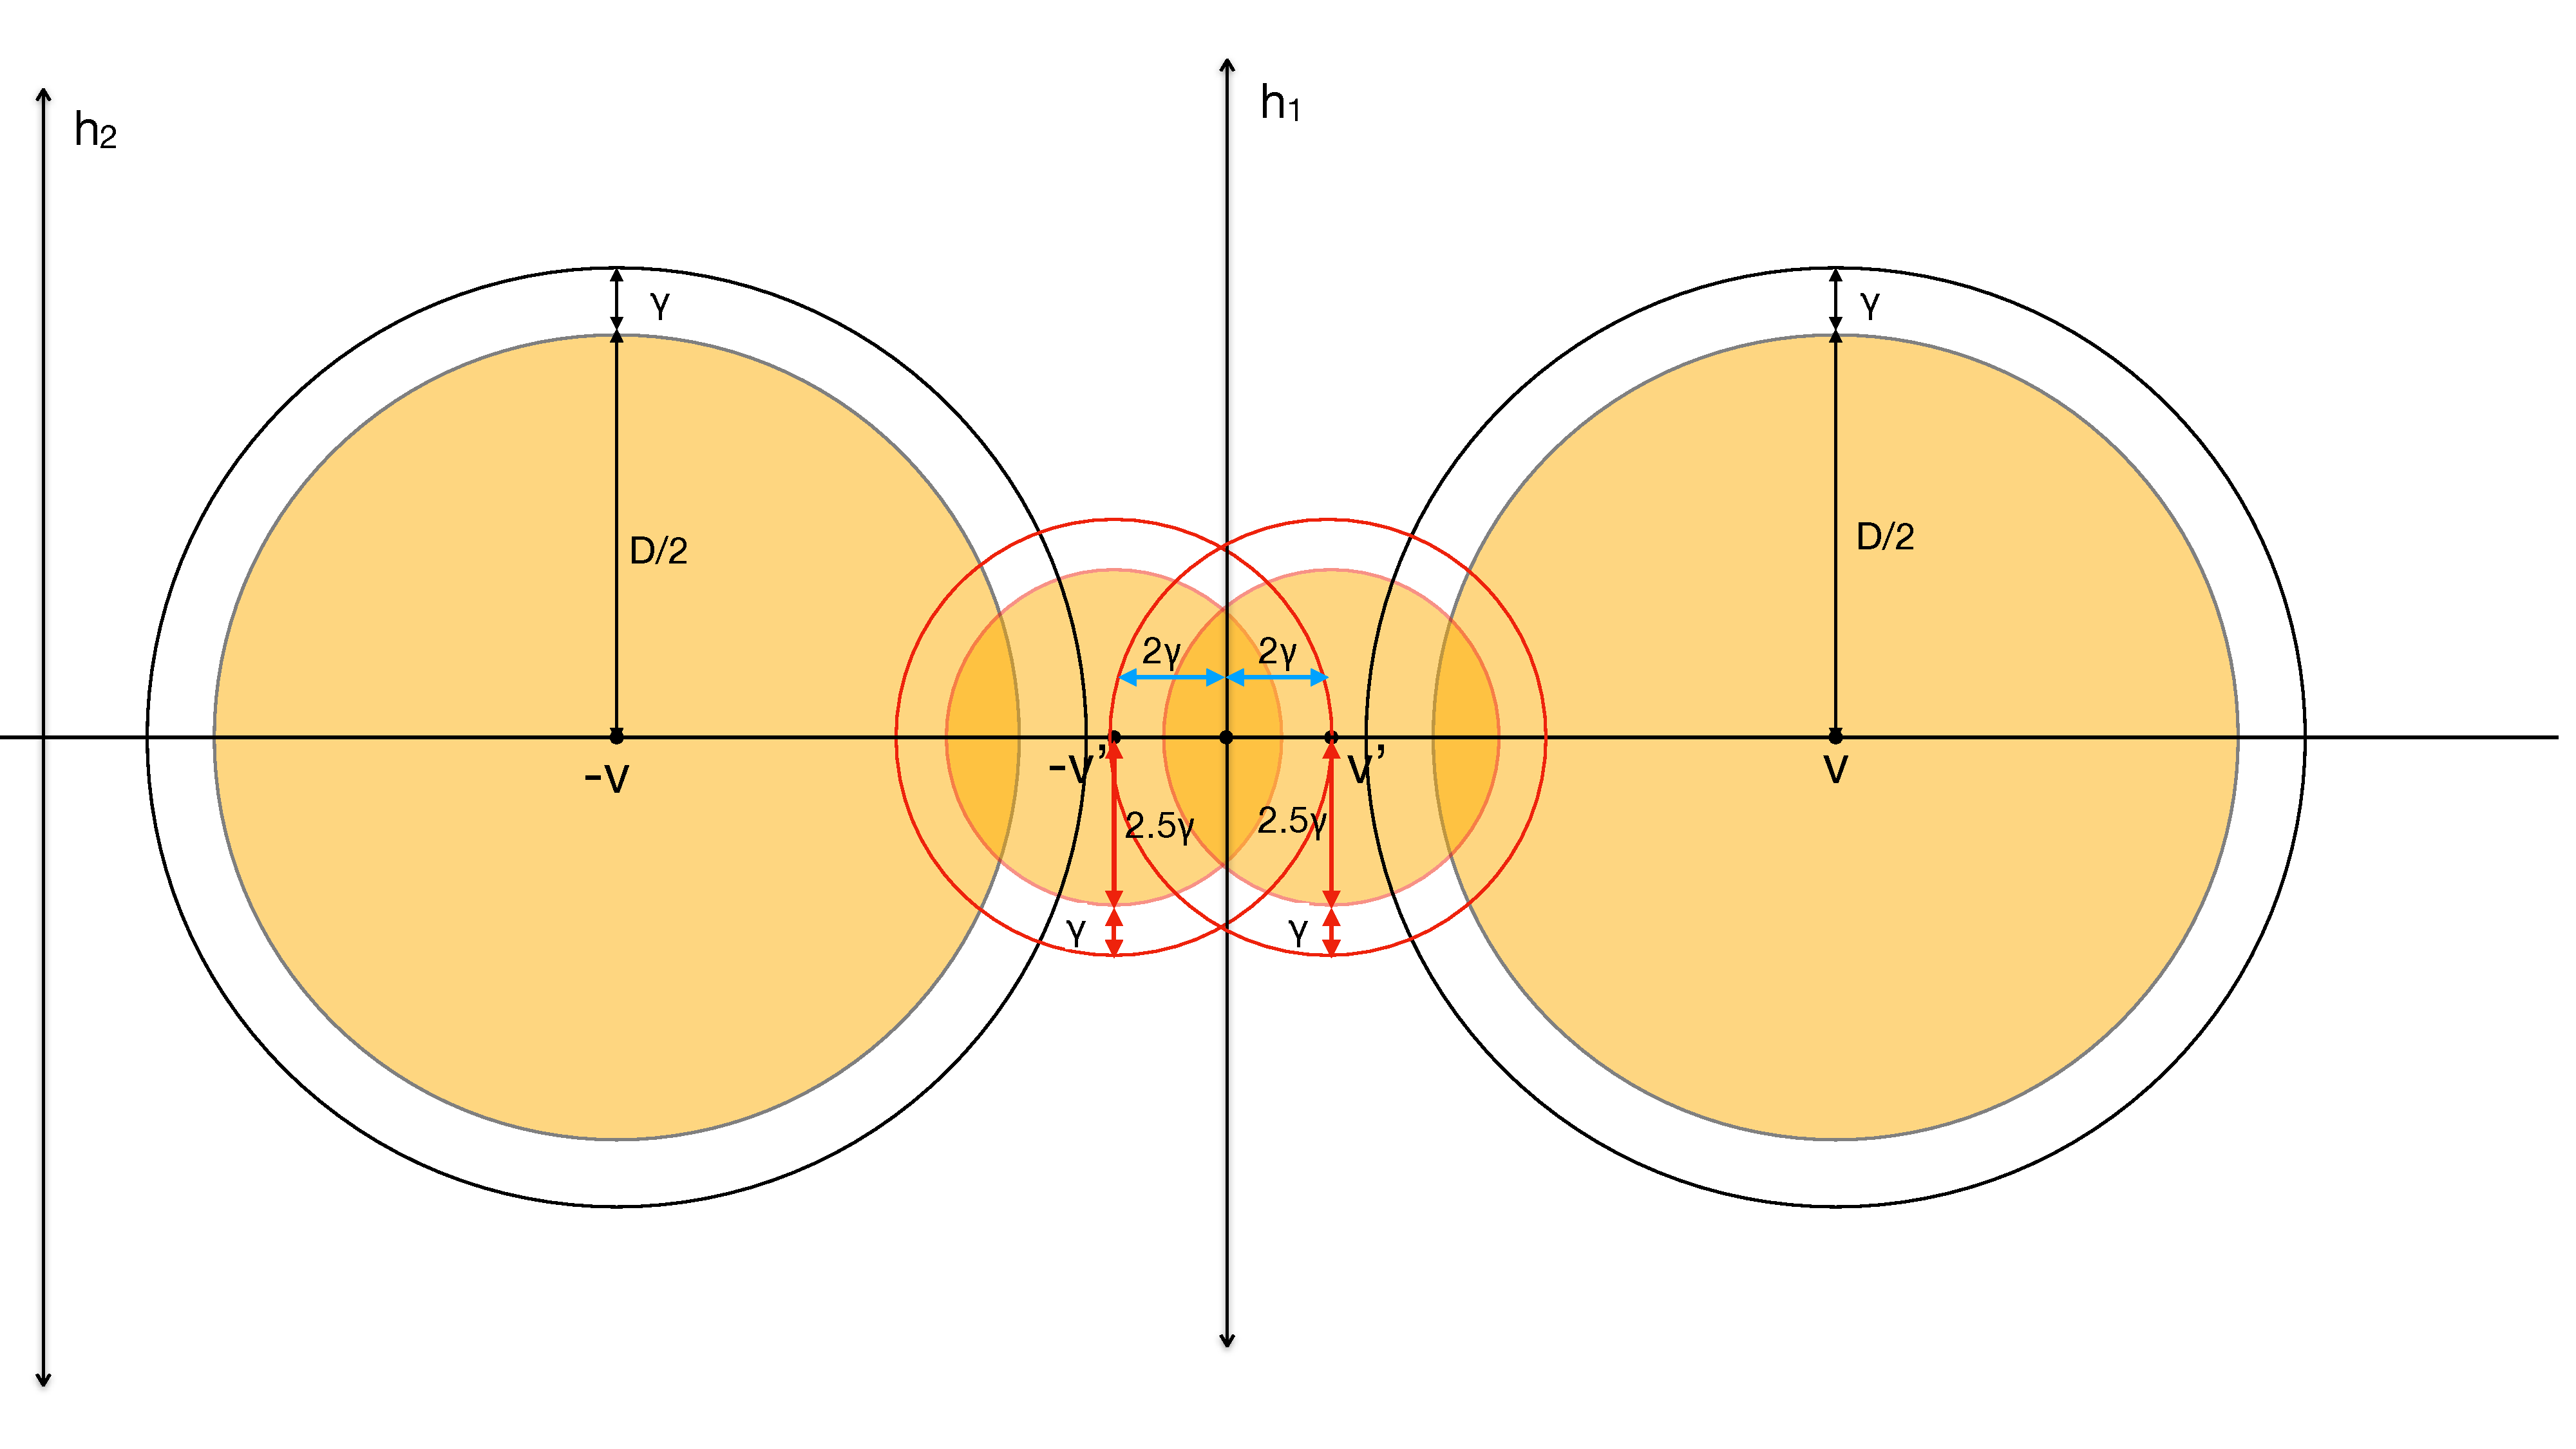
\includegraphics[width=.6\linewidth]{icml1.pdf}
	%	\caption{The generic task}
		\label{fig:LB}
	%\end{subfigure}
   \caption{Illustration for the sampling oracle lower bound in \propref{prop: lowerbound} in $\R^2$.}
	\label{fig:illustration}
\end{figure}

We now show a lower bound on the number of oracle calls required for tolerant learning in \citet{Urner22}'s sample oracle model. We first recall the model itself for completeness, focusing on the case of $(\mathbb{R}^d,\ell_2)$ endowed with the standard Lebesgue measure for simplicity.
\begin{defn}[Sampling Oracle {\cite{Urner22}}]
Let $U: \mathbb{R}^d \to P(\mathbb{R}^d)$ be any perturbation function such that $U(x)$ has finite Lebesgue measure for all $x \in \mathbb{R}^d$. The sampling oracle $\mathcal{O}_U$ inputs any $x \in \mathbb{R}^d$, and outputs a sample $y$ from the induced distribution on $U(x)$ under the Lebesgue measure.
\end{defn}
We prove that tolerant learning requires exponentially many calls to the sampling oracle.
\begin{customprop}{6}
For any $D>10\gamma > 0$, there exists a hypothesis class $\mathcal{H}$ and a set of robustness regions, $U$ such that the following holds. There exist constants $\epsilon$ and $\delta$ such that for any $n > 0$, any learner $L$ on $n$  samples that achieves 
$$\ell_U(L(S), \cD) \leq \min_{h \in \cH} \ell_{U^\gamma}(h, \cD) + \epsilon$$
with probability at least $1-\delta$ must make at least $\Omega\left(\left(\frac{D}{\gamma}\right)^d\right)$ calls to the sampling oracle for some valid data distribution $\cD$,
\end{customprop}
\begin{proof}[Proof of Proposition \ref{prop: lowerbound}]

Appealing to Yao's Minimax Principle, it is enough to find a class $\mathcal{H}$ and strategy for the adversary (over valid choices of perturbation sets and data distributions) such that any deterministic learner using at most $O((\frac{D}{\gamma})^d)$ oracle calls incurs at least constant error ($\epsilon$) over the optimum in $\mathcal{H}$ with constant probability ($\delta$). 

With this in mind, fix $D_0 =D-9\gamma$, let $r = 4\gamma$, and let $e_1$ denote the first canonical basis vector in $\R^d$. Our (marginal) data distribution will consist of two points in $\R^d$ $\curlybracket{(\frac{D_0}{2}+4\gamma)e_1,-(\frac{D_0}{2}+4\gamma)e_1}$. For the ease of notation, we denote $v \coloneqq (\frac{D_0}{2}+4\gamma)e_1$. Note, $||v- (-v)||_2 = D_0 + 2r$. We now define the underlying hypothesis class $\cH$ which consists of two linear classifiers $\cH \coloneqq \curlybracket{h_{1},h_{2}}$ such that $h_1 = sgn(\langle e_1, \cdot \rangle)$ and $h_2 = (\langle e_1, \cdot \rangle - D_0 - 4\gamma)$. Note that $h_1$ is a perpendicular bisector of the line segment joining $v$ and $-v$, and $h_2$ is parallel to $h_1$ but biased to the left of $v$.

Finally, we construct two perturbation sets with bounded diameter $U$ and $V$. Fix $v' = 2\gamma e_1$.
%points $v'$ and $-v'$ such that $v,v'$ are co-linear, $||x_1 - x_1'|| = \frac{D_0}{2} + 2\gamma$, and $||x_2 - x_2'|| = \frac{D_0}{2} + 2\gamma$. 
We define balls of radius $r>0$ for any given $x \in \R^d$ as $B_2(x, r)\coloneqq$ $\curlybracket{x' \in \R^d: ||x' - x||_2 \le r}$. First, we define a perturbation $U$ and its $\gamma$-perturbed region $U^\gamma$ as follows:
%Let the perturbation sets $U,V$ and their $\gamma$-perturbed sets for $\curlybracket{x_1,-v}$ be defined as 
\begin{gather*}
 U \coloneqq \curlybracket{U_{v},U_{-v}} \textnormal{where for any } x \in \curlybracket{v,-v}, U_{x} = B_2\paren{x, \frac{D_0}{2}},\\
 U^{\gamma}\coloneqq \curlybracket{U_{v}^\gamma,U_{-v}^\gamma} \textnormal{where for any } x \in \curlybracket{v,-v}, U_{x}^{\gamma} = B_2\paren{x, \frac{D_0}{2} +\gamma}
\end{gather*}
Similarly, we define another perturbation set $V$ and its $\gamma$-perturbed region $V^{\gamma}$:
\begin{gather*}
V\coloneqq \curlybracket{V_{v},V_{-v}} \textnormal{where for any } x \in \curlybracket{v,-v}, V_{x} = U_{x}\cup B_2\paren{x',\frac{5\gamma}{2}},\\
V^{\gamma}\coloneqq \curlybracket{V_{v}^\gamma,V_{-v}^\gamma} \textnormal{where for any } x \in \curlybracket{v,-v}, V_{x}^\gamma = U_{x}^\gamma \cup B_2\paren{x',\frac{7\gamma}{2}}
    %V \coloneqq \curlybracket{B\paren{x_1, \frac{D}{2}}\bigcup B\paren{x_1',\frac{5\gamma}{2}},B\paren{-v, \frac{D}{2}}\bigcup B\paren{x_2',\frac{5\gamma}{2}}}\\
 %V^{\gamma} \coloneqq \curlybracket{B\paren{x_1, \frac{D}{2}+\gamma}\bigcup B\paren{x_1',\frac{7\gamma}{2}},B\paren{x_2, \frac{D}{2}}\bigcup B\paren{x_2',\frac{7\gamma}{2}}}
\end{gather*}
where $x' = v'$ or $-v'$ if $x = v$ or $-v$ respectively. We assume that the perturbation set for $\R^d\setminus \curlybracket{v,-v}$ is null for simplicity. 
Observe that $\bigcap\limits_{x' \in \curlybracket{v,-v}} U_{x'} = \emptyset$ and so is the intersection of perturbations in $U^\gamma$.
%First, we note that $V$ is a $\gamma$-\textbf{perturbed regions} of $U$.
But, we note that $\bigcap\limits_{x' \in \curlybracket{v,-v}} V_{x'} \not= \emptyset$. This entire construction is illustrated in Figure \ref{fig:illustration}.
%Furthermore, we can pick $p_0$ such that the measure of the intersection of the sets $V^{\gamma}_{x_1}$ and $V^{\gamma}_{x_2}$ is upper bounded by $\paren{\frac{\gamma}{D}}^d$, i.e. $\mu\paren{V^{\gamma}_{x_1}\cap V^{\gamma}_{x_2}} \le \paren{\frac{\gamma}{D}}^d$.
% As considered in \citet{Urner22}, for a perturbation set $Z = U$ or $Z = V$, a sampling oracle samples based on the induced probability measure $P_{Z_x}^{\mu}$ over $Z_x \in Z$ as follows. For any set $Z'\subseteq Z_x$ in the $\sigma$-algebra over $Z_x$, we define 
% $P_{Z_x}^{\mu}(Z') = \frac{\mu(Z')}{\mu(Z_x)}$.

We are now ready to describe the adversary's strategy, who chooses one of $U$ or $V$ independently with probability $1/2$, and employs a single fixed choice of data distribution $\cD$ where $\Pr[Y = -1 | -v] = \Pr[Y = 1 | v] = 1$, and the marginal distribution is uniform over $v$ and $-v$. Note that if the perturbation set is $U$, then $h_1$ is optimal as $\ell_U\paren{h_1,\cD} = 0$ whereas $\ell_U\paren{h_2,\cD} = 1/2$. On the other hand if $V$ is chosen then $h_2$ is optimal as $\ell_V\paren{h_2,\cD} = \frac{1}{2}$ and $\ell_V\paren{h_1,\cD} = 1$. The idea is to show that the learner cannot distinguish between $U$ and $V$ with high probability, and thus cannot choose the right hypothesis. We note that since the data distribution is fixed and known to the learner, we only need to consider randomness over the sample oracle---labeled samples have no effect on the bound.

More formally, we split our analysis into two cases based on whether or not the learner draws an (oracle) sample in $V^\gamma \setminus U^\gamma$. First, note that conditioned on the fact that the learner draws no such sample, by construction the posterior probability of $U$ is strictly higher than that of $V$. This means the learner's expected excess error is minimized by always outputting $h_1$ on such samples. On the other hand, if the learner observes a sample in $V^\gamma \setminus U^\gamma$, they can always achieve optimal error by outputting $h_2$. 

Since the above learning rule minimizes the learner's expected excess error, it is enough to bound the expected error of this rule:
\begin{align*}
    \mathbb{E}_{Z,S \sim \mathcal{O}_Z}[OPT_Z - \ell_{Z}(\mathcal{A}(S),\cD)] &\geq \frac{1}{2}\Pr[S \subset U^\gamma \wedge Z=V]\\
    &= \frac{1}{2}\Pr[Z=V]\Pr[S \subset U^\gamma | Z=V]\\
    &= \frac{1}{4}\Pr[S \subset U^\gamma | Z=V]
\end{align*}

The key observation is then simply to notice that $\Pr[S \subset U^\gamma | Z=V]$ is constant whenever the learner draws at most $O((\frac{D}{\gamma})^d)$ oracle samples. This follows from the fact that under the induced distribution $P_{V^\gamma}$ on $V$:
\begin{equation}
 P_{V^\gamma}(V^\gamma\setminus U^\gamma) = \frac{\mu(V^\gamma\setminus U^\gamma)}{\mu(V^{\gamma})} \le \frac{\mu(B_2(v',\frac{7\gamma}{2}))}{\mu(U^\gamma_v) + \mu(B_2(v',\frac{7\gamma}{2}))} \le \frac{(\frac{7}{2}\gamma)^d}{D_0^d}\nonumber
\end{equation}
where $\mu$ is the standard Lebesgue measure. Similarly we then have
\begin{align*}
    P_{V^\gamma}(U^\gamma) \ge 1 - \frac{(\frac{7}{2}\gamma)^d}{D_0^d} \label{eq: U}
\end{align*}
and finally that
\begin{align*}
    \Pr[S \subset U^\gamma | Z=V] \geq \paren{1 - \frac{(\frac{7}{2}\gamma)^d}{D_0^d}}^{|S|}
\end{align*}
which is at least some constant when $|S| \leq c(\frac{D_0}{\gamma})^d$ for some sufficiently small absolute constant $c<0$. Since $D_0 = D - 9\gamma$, there exists $c'$ such that this holds when $|S| \leq c'(\frac{D}{\gamma})^d$ which implies the proposition.
% the probability the learner draws no sample in $V^\gamma \setminus U^\gamma$ is high.

% Fix a training sample of size $N$, say $S_N \coloneqq \curlybracket{(x_i,y_i)}_{i=1}^N$ such that the learner calls the sampling oracle for less than $Q_N = \paren{\frac{D}{\gamma}}^d$ times.

% Now, if the adversary picks the perturbation set to be $U$, then we know that the sampling oracle can sample only from $U^\gamma$. In this case, note that as the sampling oracle provides a perturbed sample from $U^\gamma$ the learner could correctly pick the optimal hypothesis $\hat{h}\coloneqq h_1$ as it distinguishes $U$ from $V$. Thus, the expected error $\ell_U(\hat{h},\cD) = 0$ if learner picks $\cA^\gamma(S_N) = h_1$, otherwise $\ell_U(h_2,\cD) = \frac{1}{2}$. 

% Consider the case that the adversary picks $V$ as the perturbation set. The sampling oracle can sample perturbed points from $V^\gamma$. First, note that for all $x \in \curlybracket{v,-v}$, $U_x^\gamma \subset V_{x}^\gamma$. Thus, it is possible that the sampling oracle samples perturbed points only from $U^\gamma$. If that is the case, then $\ell_V(\hat{h},\cD) = 1$ if $\cA^{\gamma}(S_N) = h_1$. But in case if the algorithm picks $\cA^\gamma(S_N) = h_2$ then $\ell_V(\hat{h},\cD) = \frac{1}{2}$. But then $\ell_U(\hat{h},\cD) = \frac{1}{2}$ because sampling oracle only sampled from $U^\gamma$. %Thus, the expected error over the choice of perturbation sets is $\frac{1}{2}\ell_U(\hat{h},\cD) + \frac{1}{2}\ell_V(\hat{h},\cD) \ge \frac{1}{2}$ if oracle picks points from $U^\gamma$.

% Now, consider that the sampling oracle picks perturbed points from $V^\gamma\setminus U^\gamma$. If $\cA^\gamma(S_N) = h_1$ then $\ell_V(\cA^\gamma(S_N),\cD) = 1$, otherwise $\ell_V(\cA^\gamma(S_N) = h_2,\cD) = \frac{1}{2}$. Thus, in order to minimize the error, $\cA^{\gamma}$ chooses $h_2$ upon given the training sample $S_N$.% and thus the total error $\frac{1}{2}\ell_U(\hat{h},\cD) + \frac{1}{2}\ell_V(\hat{h},\cD) = \frac{1}{4}$. 

% Note that sampling oracle can sample a perturbed point in $V^\gamma\setminus U^\gamma$ with probability
% \begin{equation}
%  P_{V^\gamma}^{\mu}(V^\gamma\setminus U^\gamma) = \frac{\mu(V^\gamma\setminus U^\gamma)}{\mu(V^{\gamma})} \le \frac{\mu(B_2(v',\frac{7\gamma}{2}))}{\mu(U^\gamma_v) + \mu(B_2(v',\frac{7\gamma}{2}))} \le \frac{(\frac{7}{2}\gamma)^d}{D^d}\nonumber
% \end{equation}
% Similarly,
% \begin{align}
%     P_{V^\gamma}^{\mu}(U^\gamma) \ge 1 - \frac{(\frac{7}{2}\gamma)^d}{D^d} \label{eq: U}
% \end{align}
% %Note that in order to sample for $V^\gamma\setminus U^\gamma$, sampling oracle has to sample perturbed examples from $V_{x_1}^{\gamma}\cap V_{x_2}^{\gamma}$. We know that $\mu\paren{V^{\gamma}_{x_1}\cap V^{\gamma}_{x_2}} \le \paren{\frac{\gamma}{D}}^d$. 
% If $Q_N \le \frac{D^d}{(\frac{7}{2}\gamma)^d}$, then using \eqref{eq: U} there is a non-trivial constant probability $p_0 > 0$ that sampling oracle picks points in $U^\gamma$. Now, we can bound the expected error over randomized choices of perturbation set as follows:
% \begin{align}
%     \expctover{S_N}{\expctover{Z\sim(U,V)}{\ell_Z(\cA^\gamma(S_N),\cD)}} &\ge P_{\cD}(\textnormal{\textbf{1}}\curlybracket{S_N \sim U^\gamma})\cdot\paren{\frac{1}{2}\ell_U(\cA^\gamma(S_N),\cD) + \frac{1}{2}\ell_V(\cA^\gamma(S_N),\cD)}\label{eq: bound1}\\
%     &\ge p_0\cdot\paren{\frac{1}{4} + \frac{1}{4}}\label{eq: bound2}\\
%     &= \frac{p_0}{2}\nonumber
% \end{align}
% In \eqnref{eq: bound1}, we consider the samples $S_N$ that fall in $U^\gamma$. In \eqnref{eq: bound2}, we note that if $\cA(S_N) = h_1$ then the expected error is $\frac{1}{2}\ell_U(h_1,\cD) + \frac{1}{2}\ell_V(h_1,\cD) \ge \frac{1}{2}$. In case, $\cA^\gamma(S_N)= h_2$ then the expected error is $\frac{1}{2}\ell_U(h_2,\cD) + \frac{1}{2}\ell_V(h_2,\cD) \ge \frac{1}{4} + \frac{1}{4} = \frac{1}{2}$. This implies that the randomized algorithm forces a lower bounded error for any deterministic tolerant algorithm $\cA^\gamma$ if $Q_N \le \frac{D^d}{(\frac{7}{2}\gamma)^d}$.
%%%%%%%%%%%%%%
%But then $\cA^\gamma$ incurs at least error $c_0\ell_V(\hat{h},\cD) > \frac{c_0}{2}$ with constant probability over the choice of $S_N$. Using Yao's minimax theorem, total expected costas argued above the total error is at least $\frac{1}{2}$ with constant probability. which implies that the tolerant algorithm $\cA^\gamma$ is forced to call the sampling oracle at least $\paren{\frac{D}{\gamma}}^d$ times in order to distinguish $V$ from $U$ in order to incur optimal error with high probability. Given that the tolerant algorithm $\cA^\gamma$ calls sampling oracle for less than $\paren{\frac{D}{\gamma}}$The probability that the sampling oracle picks points from $U^\gamma$,It is evident that to distinguish $V$ from $U$, sampling oracle needs to sample examples from $V^\gamma \setminus U^\gamma$ when the adversary picks $V$, otherwise the total error is at least $\frac{1}{2}$. 
%%%%%%%%%%%%%
%Otherwise the learner will choose $h_1$ for $V$, and incurs an expected loss of $\frac{1}{2}\times\ell_V(h_1,\cD) = \frac{1}{4}$ \textcolor{red}{HY: Again, should $\ell_V(h_1,\cD) = 1?$} and vice versa. \textcolor{red}{HY: What does vice versa mean here? When the adversary chooses $U$?}
%Irrespective of the hypothesis returned by any tolerant algorithm, adversary could also pick the perturbation set that leads to a wrong optimal.
 


%\begin{align*}
%    \expctover{Z \sim \paren{U,V}}{\ell_Z(\hat{h},\cD)} = \frac{1}{2}\ell_U(\hat{h},\cD) + \frac{1}{2}\ell_V(\hat{h},\cD)
%\end{align*}

\end{proof}

We note that in \citet{Urner22}, the sampling oracle is defined more generally for any \textit{doubling-measure} $\mu$, that is any measure for which there exists some ``doubling-constant'' $C>0$ such that for all $x \in \mathbb{R}^d$ and $r \in \mathbb{R}^+$:
\[
0 < \mu(B(x,2r)) \leq C\mu(B(x,r)) < \infty.
\]
In this more general setting, one can prove a lower bound that scales with the doubling-constant (typically exponential in the associated doubling-dimension of the metric space) simply by appropriately increasing the concentration of measure on $U^\gamma$. 


\section{Robust VC for $k$ points}\label{app: robust vc bound}
In this section, we prove that the size-$k$ perturbation sets only cost a $\log(k)$ factor over the VC dimension of the original class. To formalize this, we first recall a few basic definitions standard to the (adversarially robust) learning literature.

\begin{defn}[Robust Loss Class]
Given a hypothesis $h: \cX \to \{0,1\}$ and perturbation function $U:\cX \to P(\cX)$, let $h^\ell_U: X \times \{0,1\}$ be the function over labeled samples measuring the robust loss of $h$:
\[
h^\ell_U(x,y) = \begin{cases}
0 & \text{ if } \ \forall x' \in U(x): h(x')=y\\
1 & \text{ else.}
\end{cases}
\]
The robust loss class of $(\cX,\cH)$ is the hypothesis class over $\cX \times \{0,1\}$ given by:
\[
\mathcal{L}^U_{\cH} \coloneqq \{ h^\ell_U : h \in \cH\}.
\]
\end{defn}
We are interested in analyzing a standard complexity measure of the robust loss class called VC dimension
\begin{defn}[VC Dimension]
The VC dimension of a hypothesis class $(\cX,\cH)$ is the size of largest subset $S \subseteq \cX$ such that $\cH$ obtains all $2^{|S|}$ labelings on $S$. We say such a set is \textit{shattered} by $\cH$.
\end{defn}
% We define the robust VC dimension of a class $(X,H)$ as the VC dimension of its robust loss class.
% \begin{defn}[Robust VC Dimension]
% The robust VC dimension of a hypothesis class $(X,H)$ with respect to perturbation function $U:X \to P(X)$ is $vc(\mathcal{L}^U_H)$.
% \end{defn}
We show the VC dimension of the robust loss class incurs at most $\log(k)$ blow-up over the original class.
\begin{prop}[Overhead of Robust VC]\label{prop:finite-RVC}
Let $(\cX,\cH)$ be a hypothesis class of VC-dimension $d$ and $U: \cX \to P(\cX)$ any perturbation function with support bounded by some $k \in \mathbb{N}$. Then the VC dimension of $\mathcal{L}^U_{\cH}$ is at most $O(d\log(dk))$.
\end{prop}
This result was also independently communicated to us by Omar Montasser. The proof of Proposition \ref{prop:finite-RVC} relies on the classical Sauer-Shelah-Perles lemma, which we recall here for completeness.
\begin{lem}[Sauer-Shelah-Perles \cite{sauer1972density,shelah1972combinatorial}]
Let $(\cX,\cH)$ be a hypothesis class of VC-dimension $d$. Then for any finite subset $S \subseteq \cX$, $\cH$ obtains at most $O(|S|^d)$ distinct labelings on $S$.
\end{lem}
Proposition \ref{prop:finite-RVC} simply follows from using Sauer-Shelah-Perles to bound the total number of permissible patterns across perturbation sets of a sample in the loss space.
\begin{proof}[Proof of Proposition \ref{prop:finite-RVC}] Let $m \in \mathbb{N}$ and assume there exists a sample $S=(x_1,y_1), \ldots, (x_m,y_m)$ that is shattered by $\mathcal{L}^U_{\cH}$. We will show $m \leq O(d\log(kd))$. With this in mind, let $T=\bigcup_{i=1}^m U(x_i)$ denote the set of at most $km$ points corresponding to the robustness regions of our sample. The key observation is the following (essentially trivial) claim:
\begin{claim}
Any two $g_{U}^\ell,h_{U}^\ell \in \mathcal{L}^U_{\cH}$ that give distinct labelings of $S$ correspond to $g,h \in \cH$ with distinct labelings of $T$.
\end{claim} 
By robust shattering, there exist $2^m$ distinct labelings of $S$ by $\mathcal{L}^U_{\cH}$, so the above claim implies $\cH$ must have $2^m$ distinct labelings of $T$. However the latter has at most $O((km)^d)$ labelings by VC dimension, so
\[
2^m \leq O((km)^d) \Rightarrow m \leq O(d\log(dk))
\]
by standard manipulations. Finally, we note the claim is immediate from definition, since the behavior of a function $h_U^\ell \in \mathcal{L}^U_{\cH}$ on $S$ depends only on the labels of its corresponding hypothesis $h \in \cH$ on $T$ by definition. 
\end{proof}

\section{Proof of Theorem \ref{thm:upper_bound_general}}\label{sec:proof_extension}

We begin by defining $v_{ball}$, which is the adversarial VC dimension when the robustness regions are all balls of a fixed radius. We start by precisely defining these robustness regions. 

\begin{defn}
Let $U^r$ be the set of robustness regions defined by $\{U_x^r = B(x, r)\}$, where $B(x, r)$ denotes the closed ball of $\ell_2$-radius $r$ centered at $x$. 
\end{defn}

We now define the adversarial VC dimension of a set of classifiers $\cH$ for a fixed set of regions, $U^r$.

\begin{defn}
Let $\cH$ be a set of classifier. Then the adversarial VC dimension of $\cH$ with respect to $U^r$ is the maximum integer $v$, for which there exist $v$ labeled points, $(x_1, y_1), \dots, (x_r, y_r)$ so that for any subset $S \subset \{(x_1, y_1) ,\dots, (x_r, y_r)\}$, there exists $h_S \in \cH$ with $$\ell(h_S, (x_i, y_i) = \begin{cases}0 & i \in S \\ 1 & i \notin S\end{cases}.$$ We denote this by $v_{ball}^r$.
\end{defn}

Finally, we define $v_{ball}$ as the maximum value of $v_{ball}^r$ over all $r > 0$. Note that this quantity has been well studied -- for example \cite{Cullina18} shows that for linear classifiers, $v_{ball} = O(d)$. 

\paragraph{Proving Theorem \ref{thm:upper_bound_general}} We now turn our attention towards the proof. The key observation is that the main steps from the proof of Theorem \ref{thm:upper_bound1} \textit{perfectly} carry over. In particular, Lemma \ref{lem:r_works} exactly holds in this setting, and the argument given in the proof of Theorem \ref{thm:upper_bound1} also holds provided that an appropriate choice of $V$ exists. The only issue arises from Lemma \ref{lem:v_construct}, which requires that $\cH$ be regular. To remedy this, we now state and prove a different version of this lemma that uses a union of balls (of fixed radius) for $V_x$ rather than a finite set of points. 

\begin{lem}\label{lem:v_construct_new}
Let $\cH$ by an arbitrary hypothesis class. For all $r \in [\frac{\epsilon\delta\gamma}{7}, \gamma]$, let $\alpha$, $U^r$ and $U^{r-\alpha}$ be as described in the proof of Theorem \ref{thm:upper_bound1}. Then there exists a set of robustness regions $V^r = \{V_x^r: x \in \reals^d\}$ satisfying the following two properties.  
\begin{enumerate}
	\item $V_x^r$ is a union of $O\left(\left(\frac{D}{\epsilon\delta\gamma}\right)^d\right)$ balls of radius , where $D$ denotes the maximum diameter of $U_x$. 
	\item Let $\alpha = \frac{\epsilon\delta\gamma}{7}$. For all labeled points $(x,y)$ and for all classifiers $h \in \cH$, $$\ell_{U^{r - \alpha}}(h, (x,y)) \leq \ell_{V^r}(h, (x,y)) \leq \ell_{U^r}(h, (x,y)).$$
\end{enumerate}
\end{lem}

\begin{proof}
Since $U_x^{r-\alpha}$ has diameter at most $D$, it follows that it can be covered with $O\left(\left(\frac{D}{\epsilon\delta\gamma}\right)^d\right)$ balls of radius $\frac{\alpha}{2}$. We let $V_x^r$ be any such cover that is minimal (meaning that (1.) is satisfied), meaning that each ball intersects $U_x^{r-\alpha}$. It follows that for all $x$, $U_x^{r-\alpha} \subseteq V_x^r \subseteq U_x^r$, which immediately implies (2.) and completes the proof. 
\end{proof}

Finally, to prove Theorem \ref{thm:upper_bound_general}, we note that the proof of Theorem \ref{thm:upper_bound1} essentially works. The only differences are that instead of bounding the robust VC dimension of $\cH$ with respect to $V_X$ in terms of $v$, we must use $v_{ball}$ as we are now considering unions of balls rather than points. As a detail, note that we are using the following minor modification of Proposition \ref{prop:finite-RVC} to bound the robust VC dimension of unions of balls using the robust VC dimension for balls. 
\begin{prop}
Let $(\cX,\cH)$ be a hypothesis class whose robust loss class with respect to $r$-balls has VC dimension $v_{\text{ball}}^r$. Then the loss class of $(\cX,\cH)$ with respect to perturbations that are a union of at most $k$ $r$-balls has VC dimension at most $O(v_{\text{ball}}^r\log(v_{\text{ball}}^rk))$.
\end{prop}
\begin{proof}
The proof is largely the same as \ref{prop:finite-RVC}. Denote the original perturbation family as $U$, and the $k$-union perturbation family by $U^k$. Given a sample $S=(x_1,y_1),\ldots,(x_m,y_m)$, let $C_i$ denote the centers of the at most $k$ balls appearing in the perturbation set of $x_i$. It is enough to observe that any two distinct labelings of $S=(x_1,y_1),\ldots,(x_m,y_m)$ by $\mathcal{L}^{U^k}_{\cH}$ correspond to distinct labelings of the extended sample $T=\bigcup_{i=1}^m (C_i,y_i)$ with respect to $\mathcal{L}^{U}_{\cH}$, where $(C_i,y_i)$ denotes the sample $\bigcup_{c \in C_i} (c,y_1)$. The bound then follows from the same double counting argument as in Proposition \ref{prop:finite-RVC}.
\end{proof}












 
%\include{chapters/chapter5/appendix5}

% Stuff at the end of the dissertation goes in the back matter
\backmatter
\bibliographystyle{unsrtnat} % Or whatever style you want like plainnat
\bibliography{references}

\end{document}
